\section*{1. Purpose and protocol}
A neural network replaces the cable-force command of the compensated PID teacher. The 21--64--64--1 tanh network is trained to imitate recorded teacher forces. During OpenSim testing, learned weights remain fixed and no PID force fallback is used.
Whole episodes retain their original training, validation, or test labels. Training updates weights; validation chooses the checkpoint; the held-out test set evaluates the selected model. Only accepted, compatible PID episodes are included. The original acceptance gate is motion RMSE $\leq2^\circ$ and full-episode maximum error $\leq5^\circ$; this gate does not imply that every accepted episode has the same accuracy.
Training minimizes normalized force error, $\mathcal{L}=\frac{1}{N}\sum_i[(\hat F_i-F_i^{\mathrm{PID}})/650]^2$. Scaling uses fixed physical units. Actual actuator commands are clipped to $[0,650]$ N.
\begin{center}\begin{tabular}{lrr}\toprule Split & Accepted episodes & Time samples\\\midrule
train & 126 & 462710\\
validation & 27 & 97250\\
test & 27 & 98916\\
\bottomrule\end{tabular}\end{center}
Counts are actual accepted episodes, so percentages can differ from the planned 70/15/15 allocation. Exact episode IDs and hashes are provided in the accompanying split manifest.
\section*{2. Learning and force prediction}
Training logged 196 epochs. The lowest logged validation force RMSE was 0.29745 N at epoch 171. This is a force-imitation measure, not an angle-tracking measure.
\begin{center}\begin{tabular}{lrrrr}\toprule Split & RMSE (N) & MAE (N) & Max. error (N) & $R^2$\\\midrule
training & 0.2984 & 0.1591 & 28.935 & 0.99999\\
validation & 0.29745 & 0.16671 & 25.543 & 0.99999\\
test & 0.28423 & 0.16171 & 24.072 & 0.99999\\
\bottomrule\end{tabular}\end{center}
\begin{figure}[H]\centering
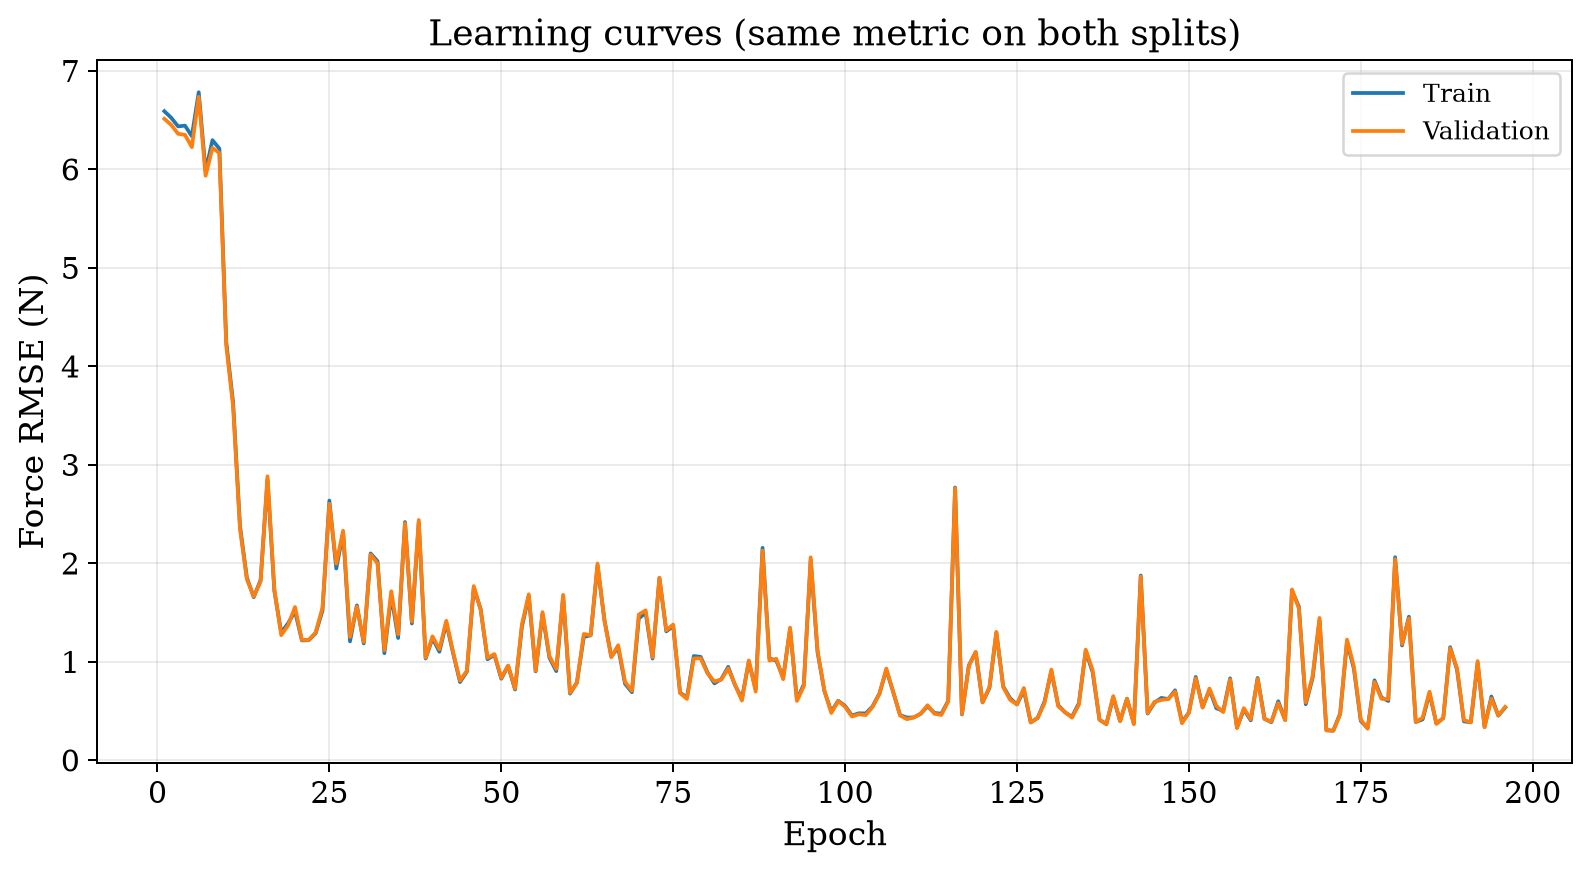
\includegraphics[width=\linewidth,height=0.69\textheight,keepaspectratio]{overleaf_figures/learning_curve.png}
\caption{Training and validation force RMSE per epoch. Validation selects the saved checkpoint; the test set is not used for selection.}
\label{fig:learning_curve}
\end{figure}
\begin{figure}[H]\centering
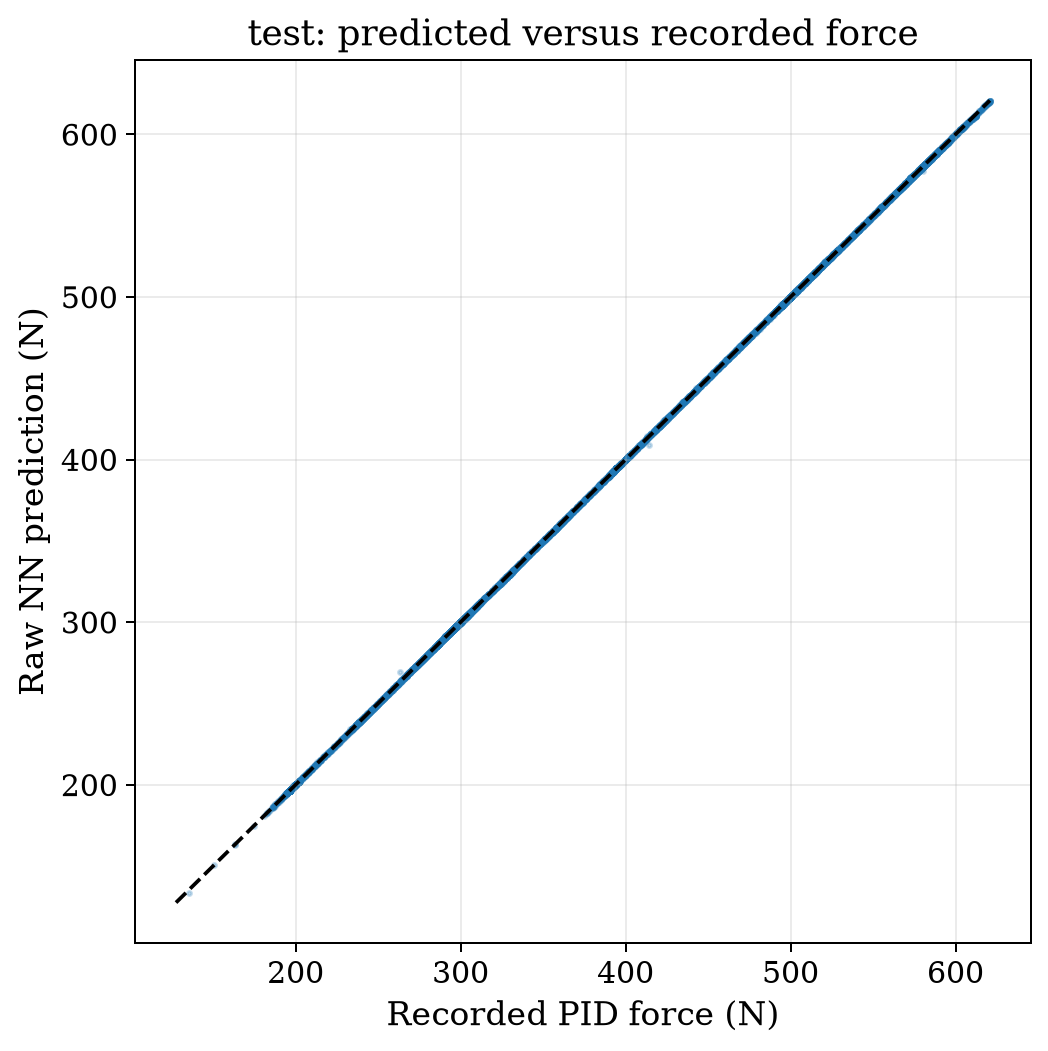
\includegraphics[width=\linewidth,height=0.69\textheight,keepaspectratio]{overleaf_figures/test_parity.png}
\caption{Predicted versus recorded compensated-PID force. Agreement with the diagonal indicates accurate force imitation; it does not by itself establish closed-loop tracking.}
\label{fig:test_parity}
\end{figure}
\begin{figure}[H]\centering
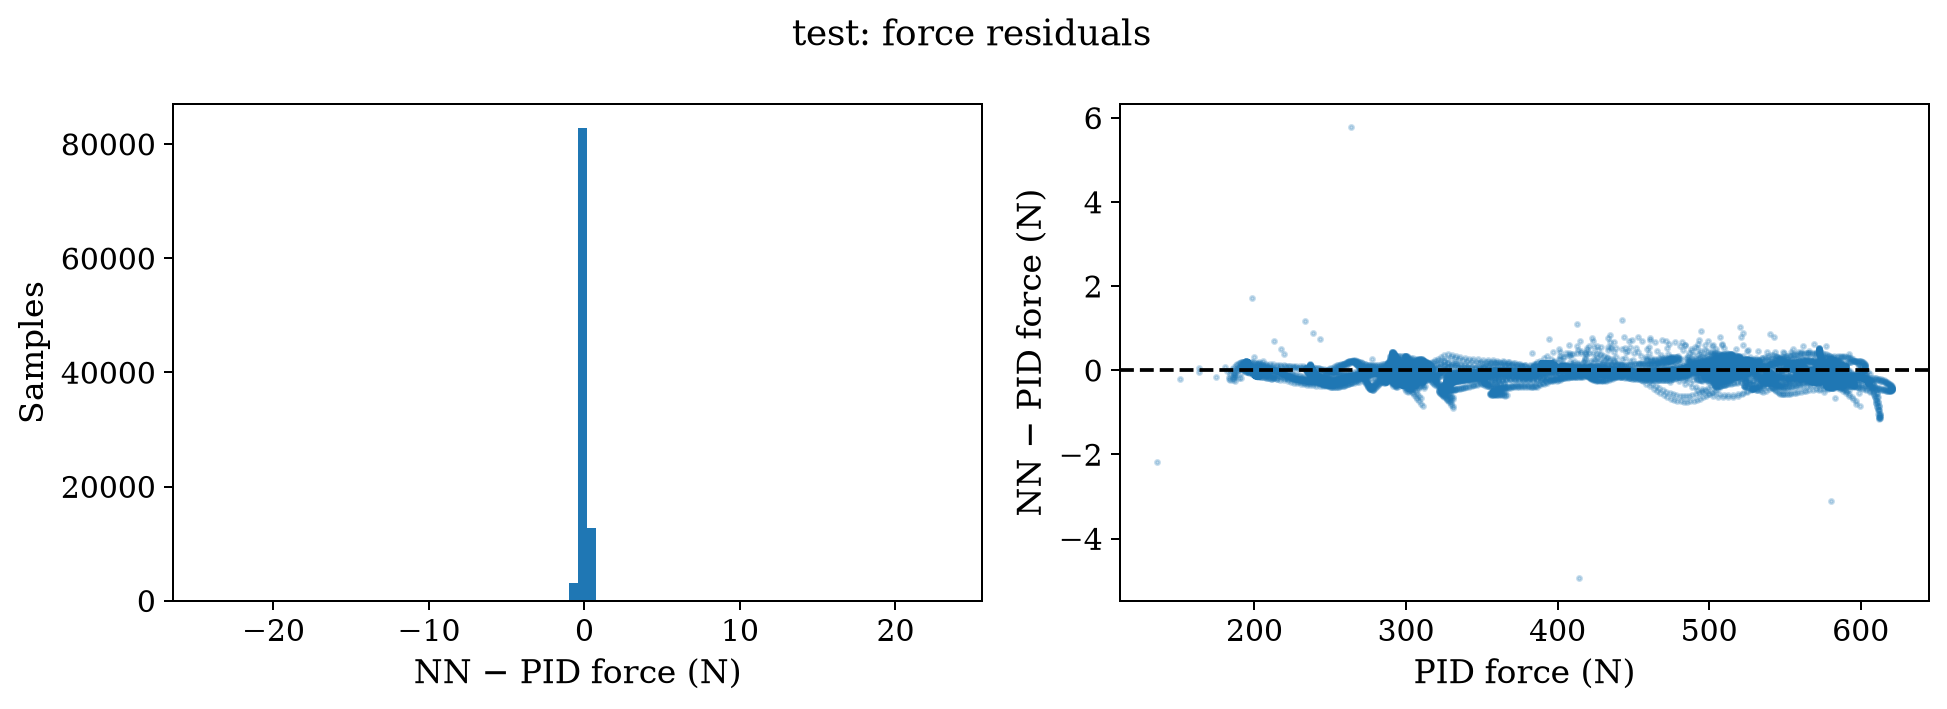
\includegraphics[width=\linewidth,height=0.69\textheight,keepaspectratio]{overleaf_figures/test_residuals.png}
\caption{Force residuals (NN minus recorded PID). The distribution and force-dependent scatter expose bias and large errors.}
\label{fig:test_residuals}
\end{figure}
\section*{3. Closed-loop OpenSim tracking}
27/27 attempted episodes completed; 27/27 met the configured acceptance gate. Failed attempts remain in the results. Motion RMSE is evaluated during motion, whereas full maximum error also includes the initial transient and holds.
The arithmetic mean of episode motion RMSEs was 0.0039848 degrees for the recorded teacher and 0.0058981 degrees for the NN; these are not sample-pooled RMSEs. The largest recorded NN full-episode error was 0.94228 degrees. These figures summarize the available 27 paired episodes.
\begin{figure}[H]\centering
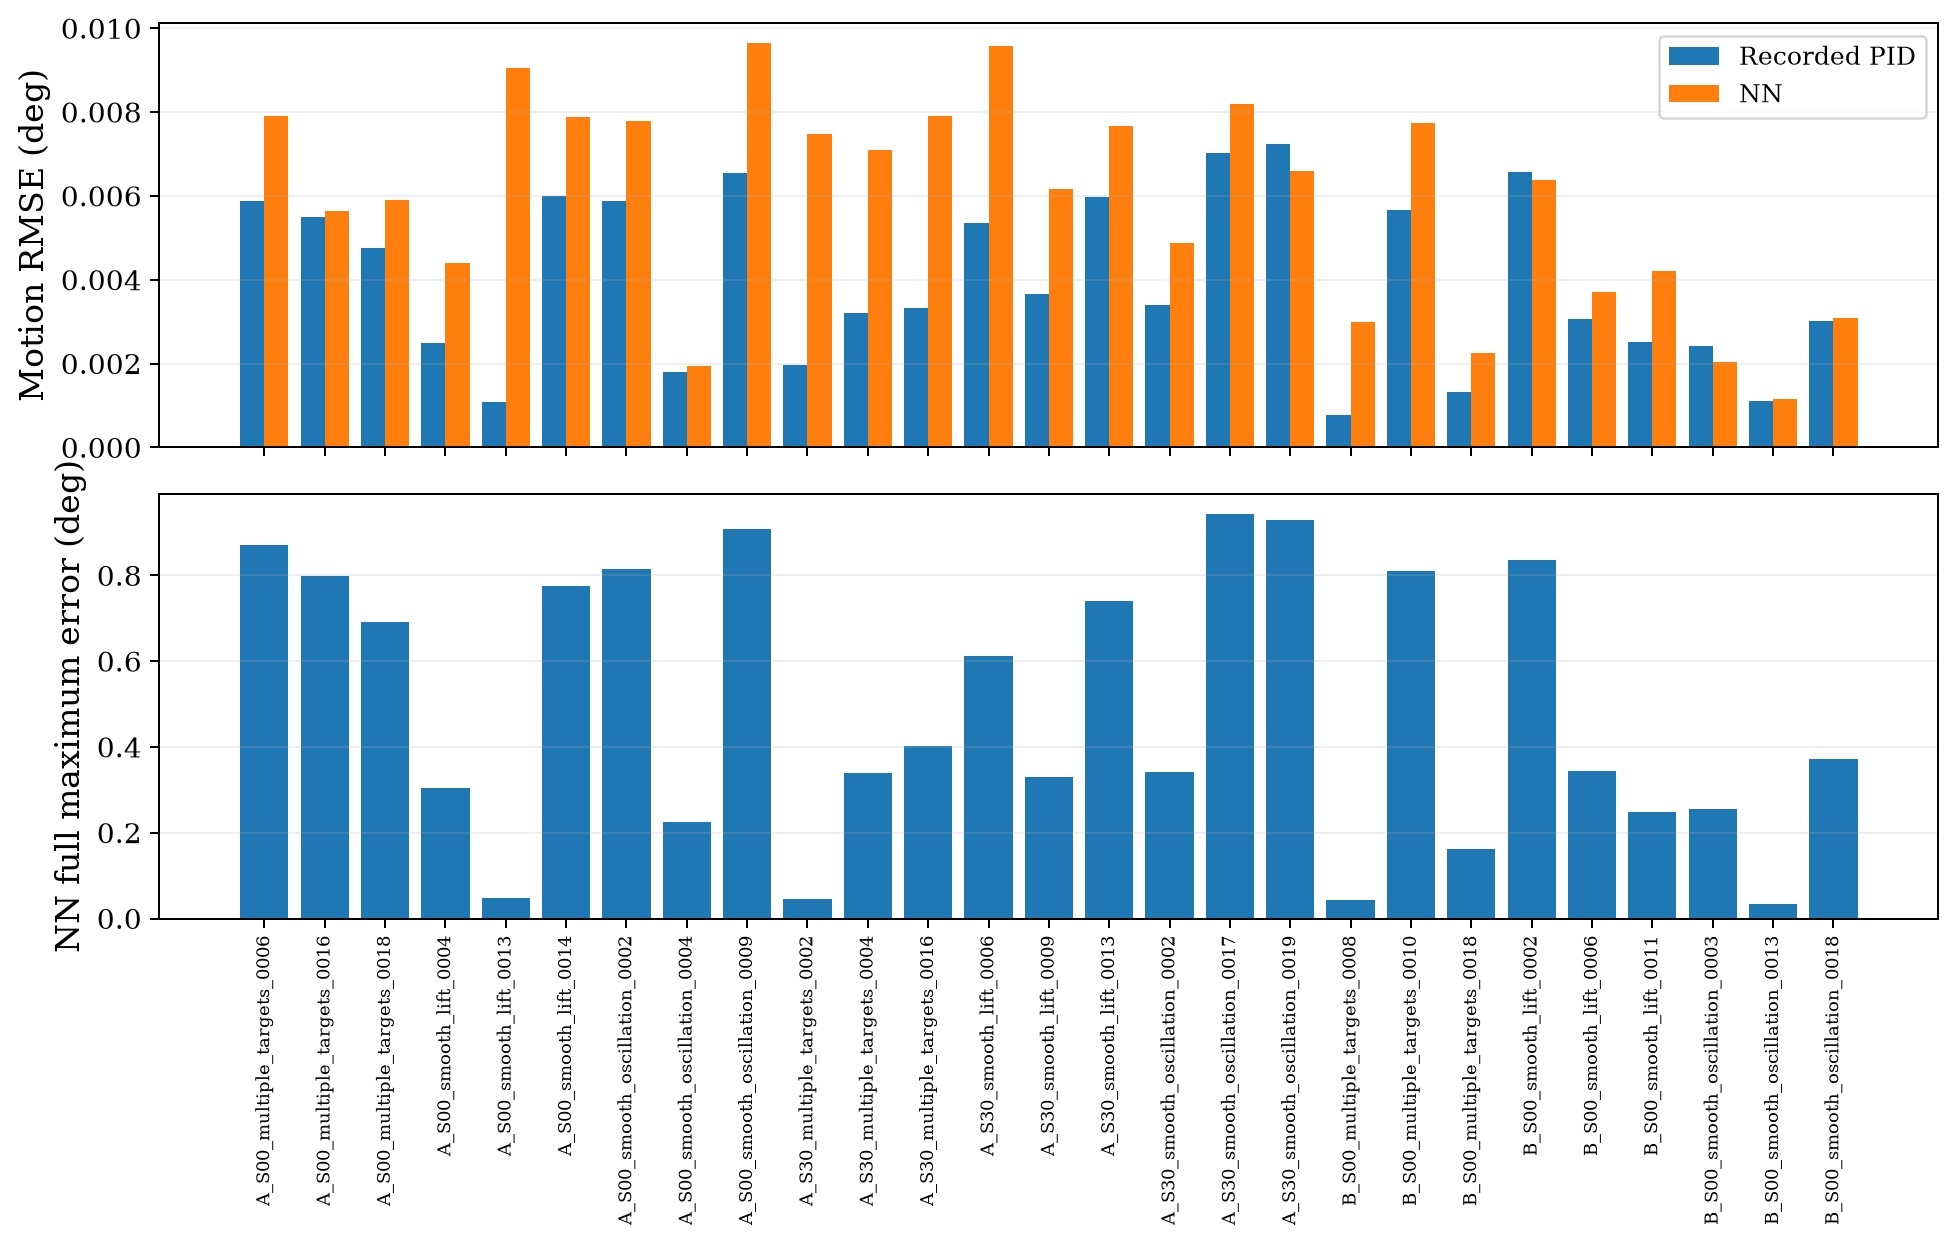
\includegraphics[width=\linewidth,height=0.69\textheight,keepaspectratio]{overleaf_figures/tracking_evidence.png}
\caption{Tracking accuracy across every evaluated episode. Motion RMSE excludes the configured holds; maximum error covers the complete recorded episode.}
\label{fig:tracking_evidence}
\end{figure}
\begin{figure}[H]\centering
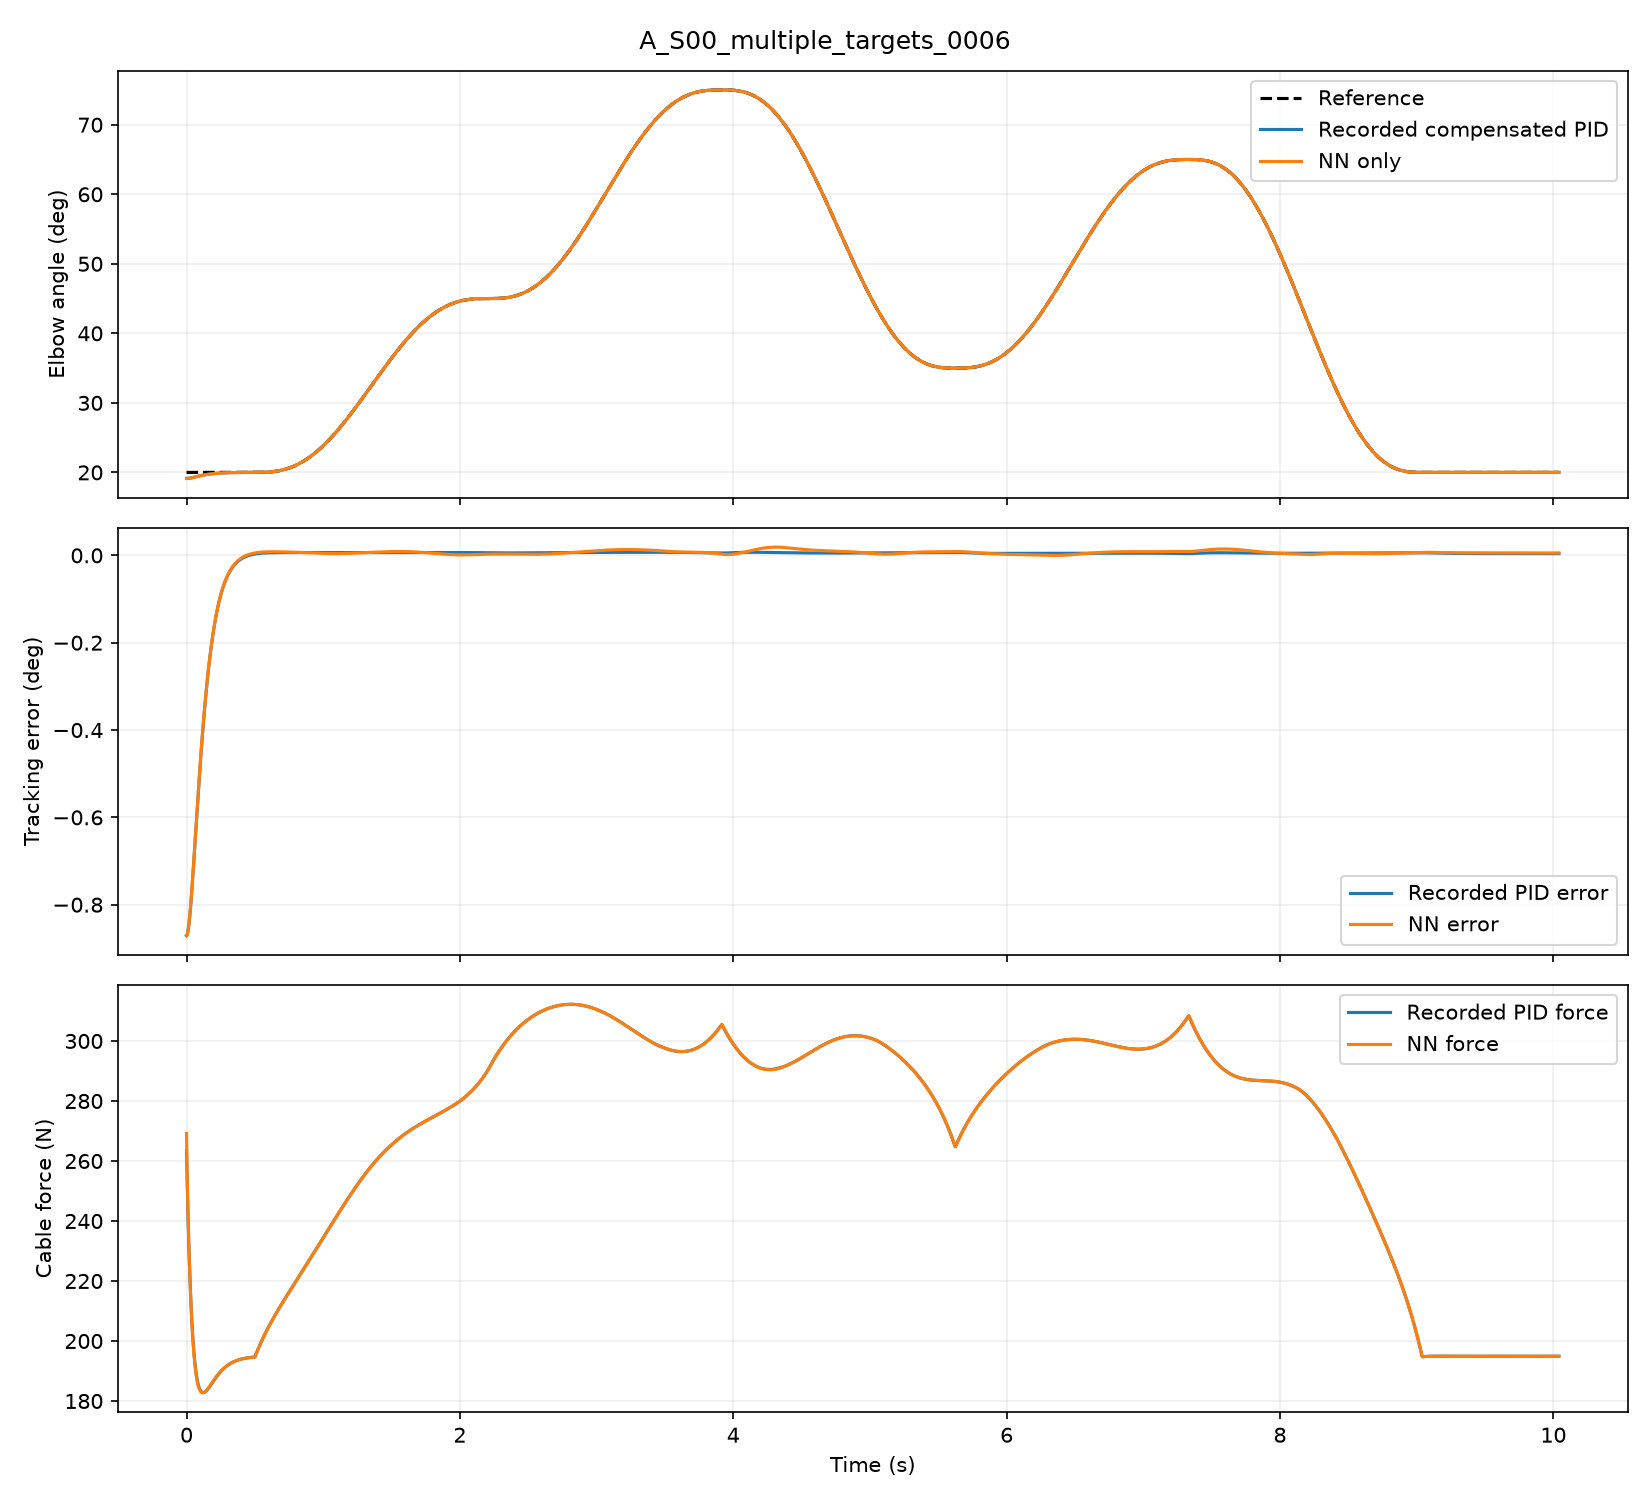
\includegraphics[width=\linewidth,height=0.69\textheight,keepaspectratio]{overleaf_figures/tracking_A_S00_multiple_targets_0006_comparison.png}
\caption{Example A\_S00\_multiple\_targets\_0006. Held-out OpenSim rollout: reference, recorded PID, and NN elbow motion; tracking errors; and cable forces. The NN supplies the cable command without a PID fallback.}
\label{fig:tracking_A_S00_multiple_targets_0006_comparison}
\end{figure}
\begin{figure}[H]\centering
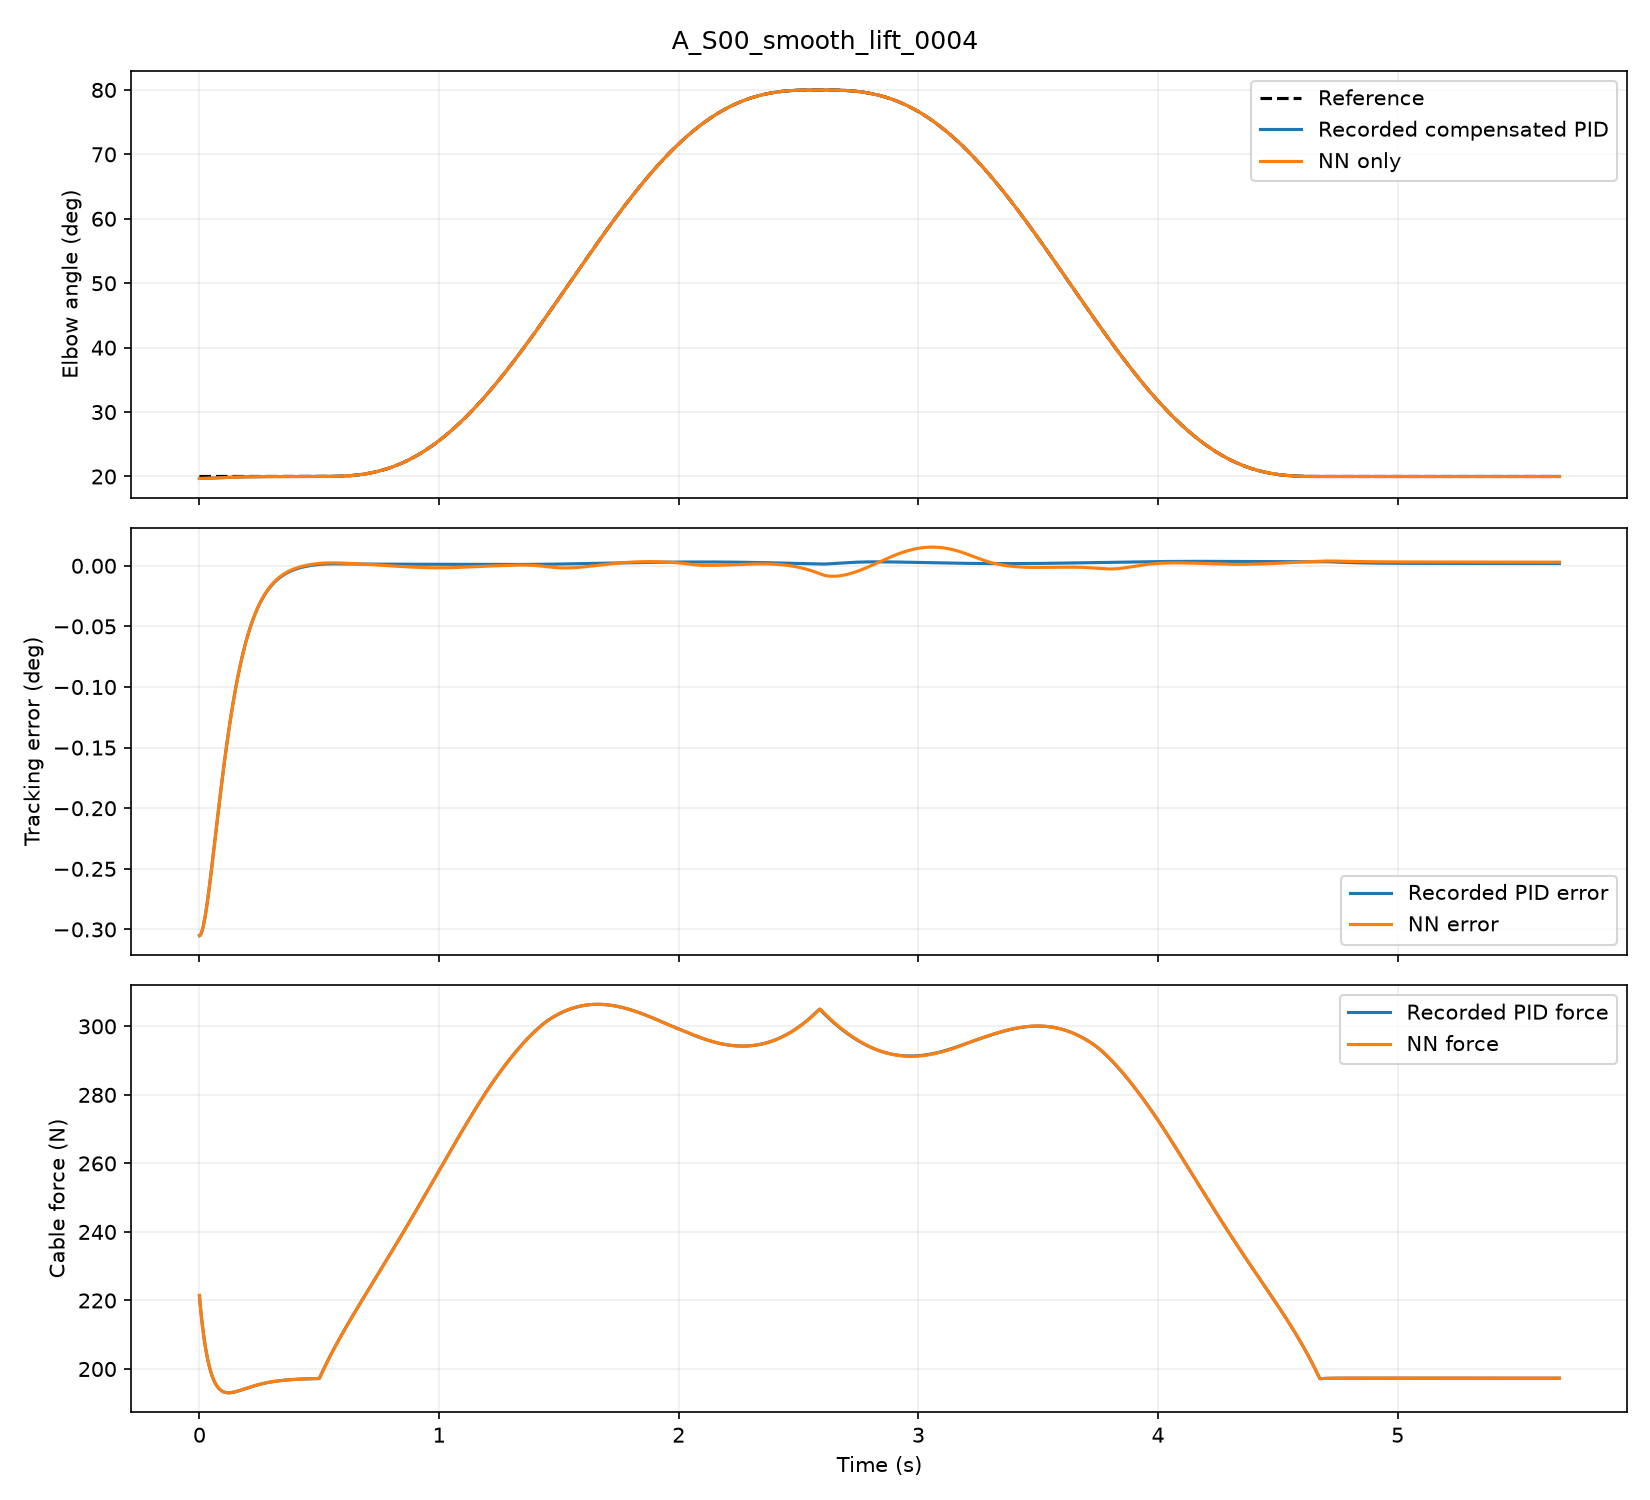
\includegraphics[width=\linewidth,height=0.69\textheight,keepaspectratio]{overleaf_figures/tracking_A_S00_smooth_lift_0004_comparison.png}
\caption{Example A\_S00\_smooth\_lift\_0004. Held-out OpenSim rollout: reference, recorded PID, and NN elbow motion; tracking errors; and cable forces. The NN supplies the cable command without a PID fallback.}
\label{fig:tracking_A_S00_smooth_lift_0004_comparison}
\end{figure}
\begin{figure}[H]\centering
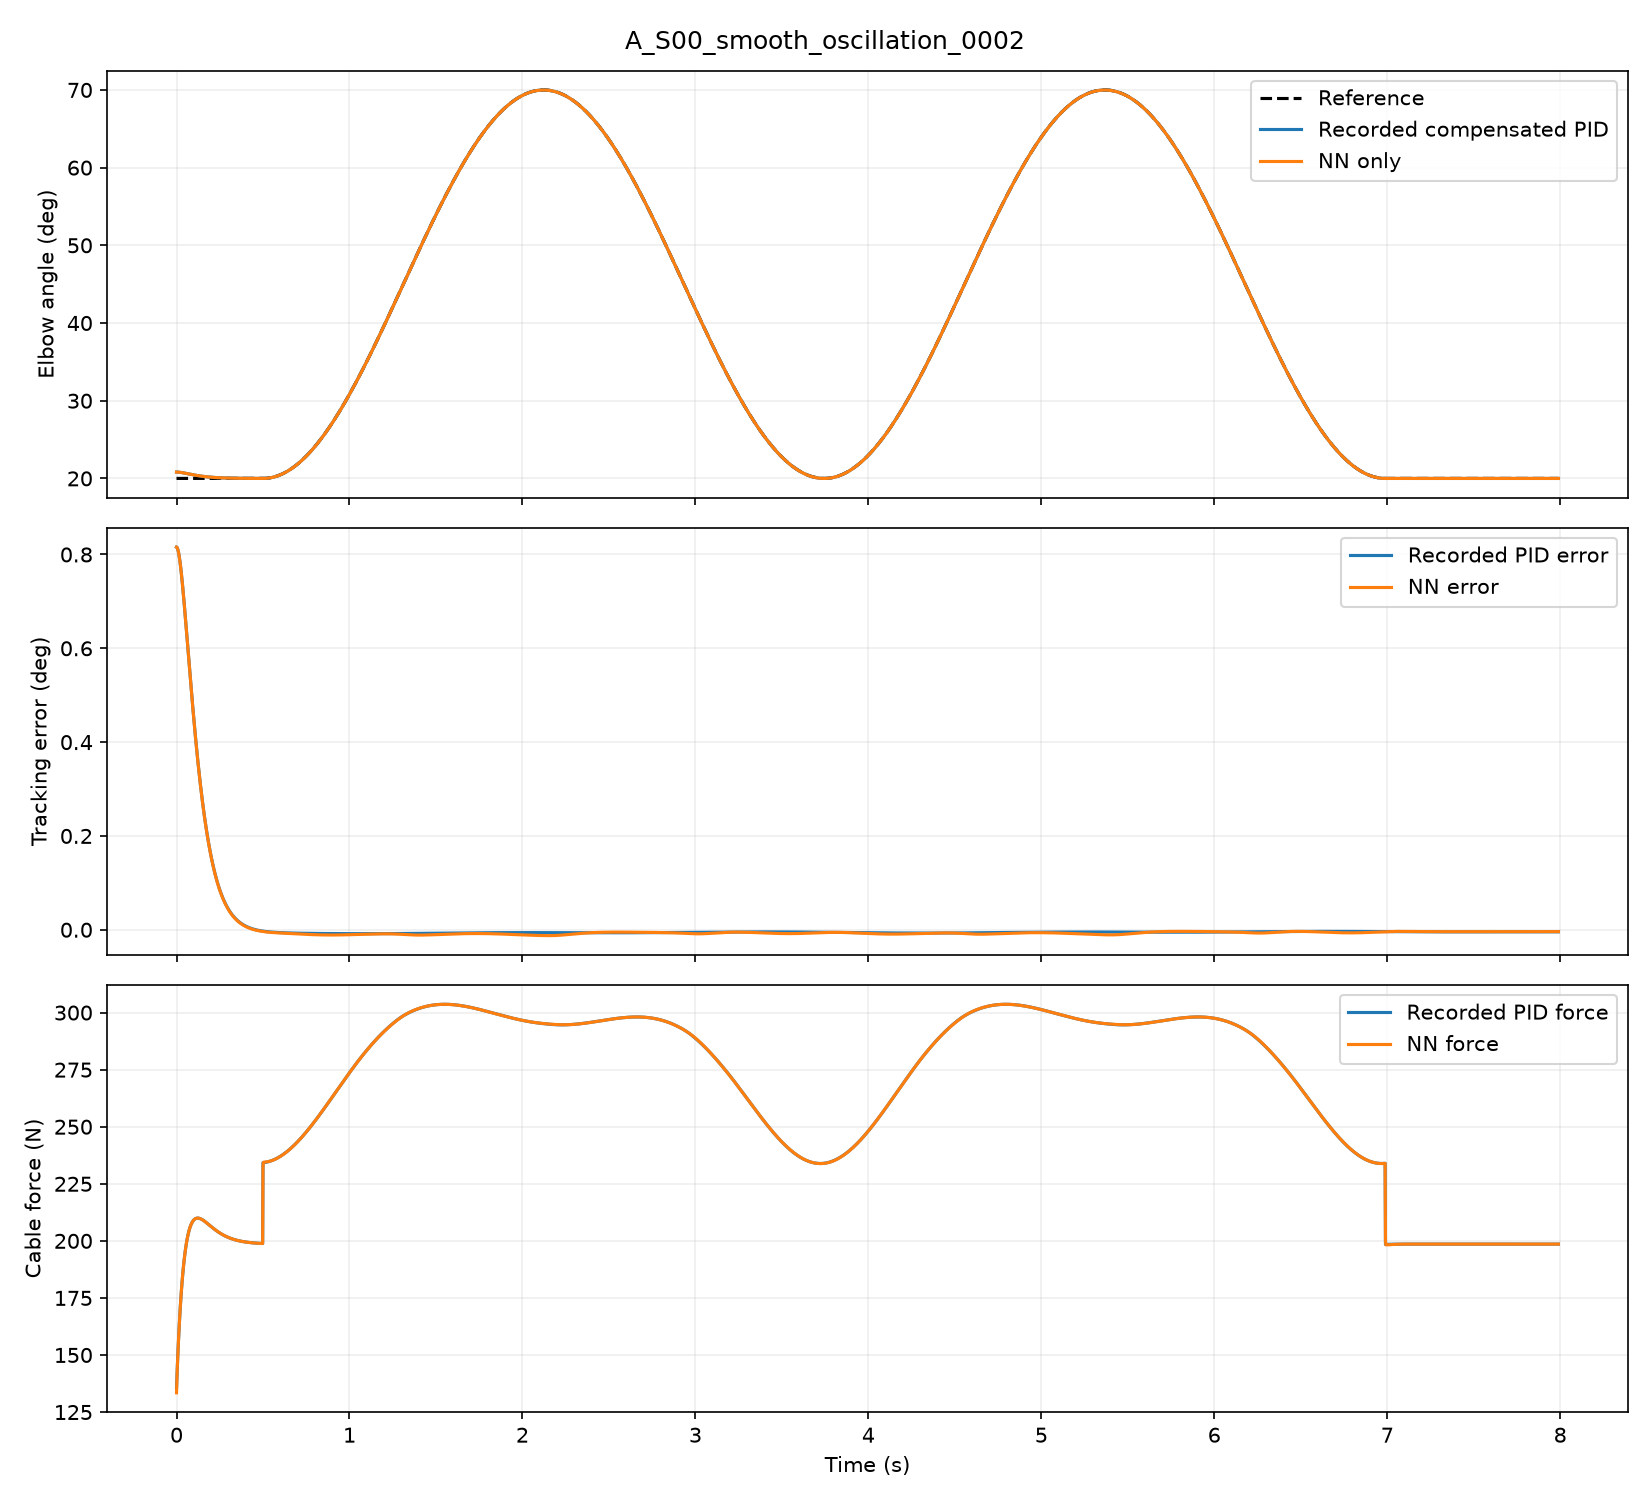
\includegraphics[width=\linewidth,height=0.69\textheight,keepaspectratio]{overleaf_figures/tracking_A_S00_smooth_oscillation_0002_comparison.png}
\caption{Example A\_S00\_smooth\_oscillation\_0002. Held-out OpenSim rollout: reference, recorded PID, and NN elbow motion; tracking errors; and cable forces. The NN supplies the cable command without a PID fallback.}
\label{fig:tracking_A_S00_smooth_oscillation_0002_comparison}
\end{figure}
\begin{figure}[H]\centering
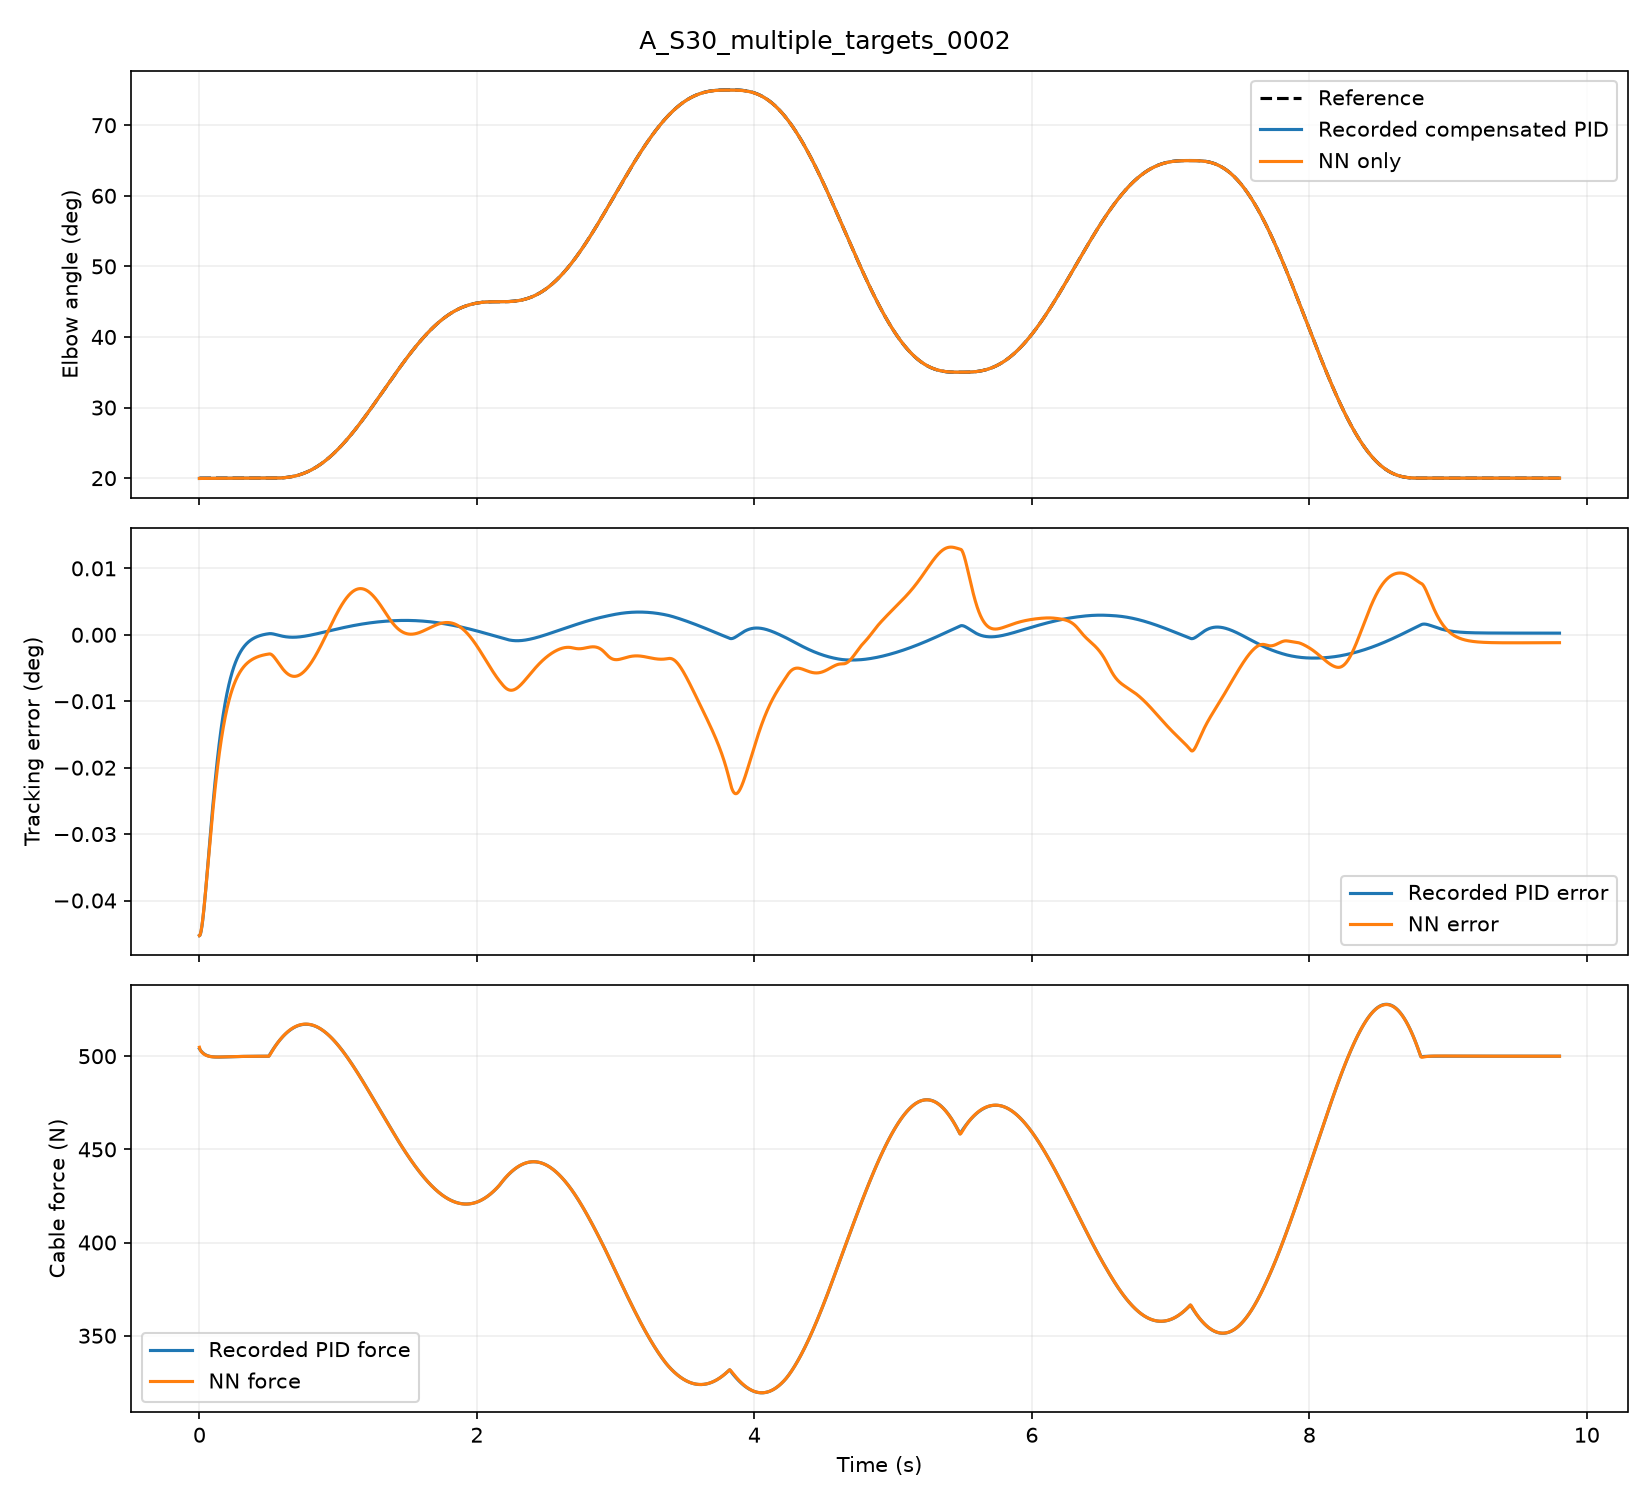
\includegraphics[width=\linewidth,height=0.69\textheight,keepaspectratio]{overleaf_figures/tracking_A_S30_multiple_targets_0002_comparison.png}
\caption{Example A\_S30\_multiple\_targets\_0002. Held-out OpenSim rollout: reference, recorded PID, and NN elbow motion; tracking errors; and cable forces. The NN supplies the cable command without a PID fallback.}
\label{fig:tracking_A_S30_multiple_targets_0002_comparison}
\end{figure}
\begin{figure}[H]\centering
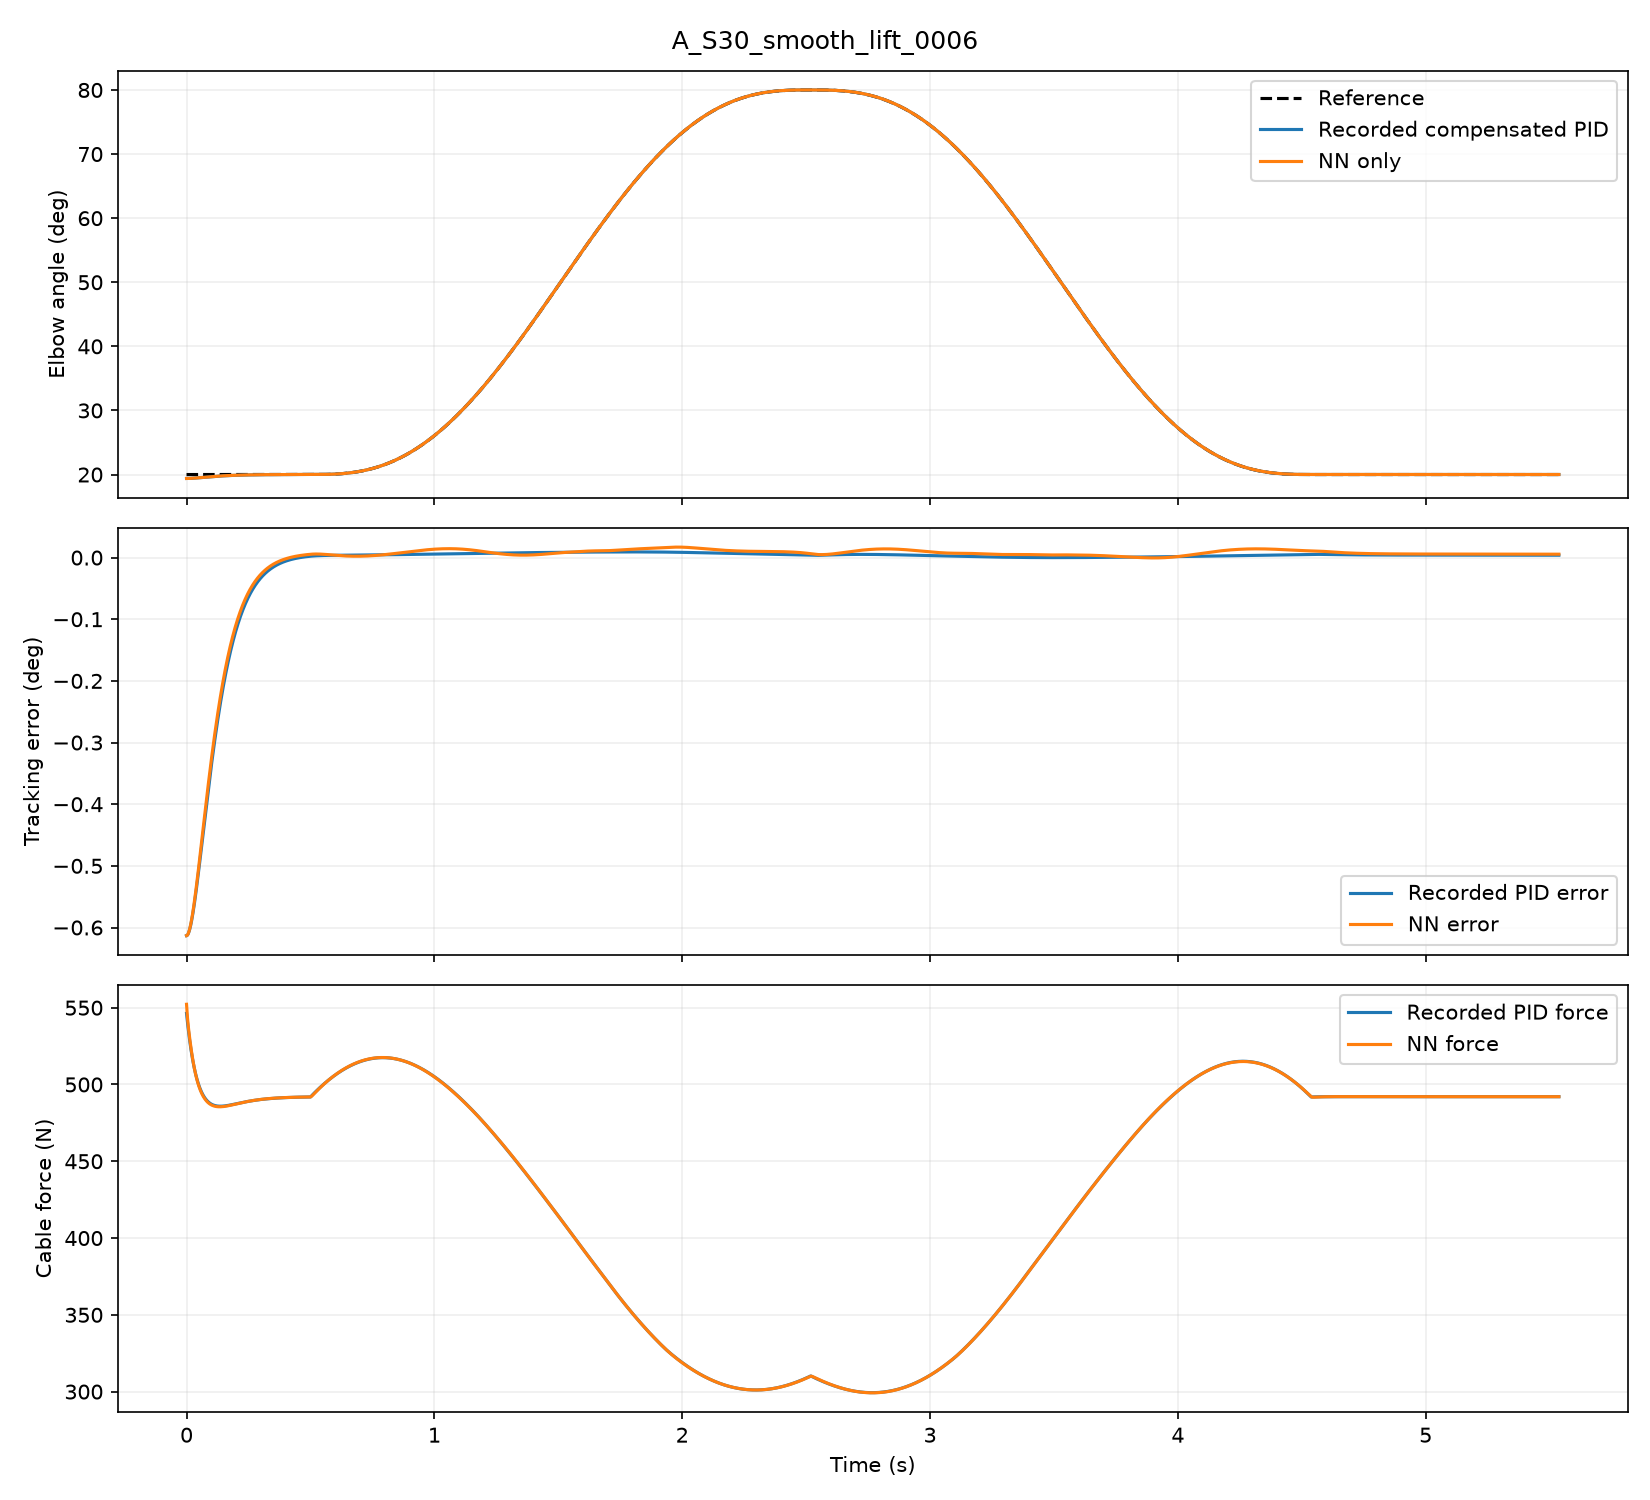
\includegraphics[width=\linewidth,height=0.69\textheight,keepaspectratio]{overleaf_figures/tracking_A_S30_smooth_lift_0006_comparison.png}
\caption{Example A\_S30\_smooth\_lift\_0006. Held-out OpenSim rollout: reference, recorded PID, and NN elbow motion; tracking errors; and cable forces. The NN supplies the cable command without a PID fallback.}
\label{fig:tracking_A_S30_smooth_lift_0006_comparison}
\end{figure}
\begin{figure}[H]\centering
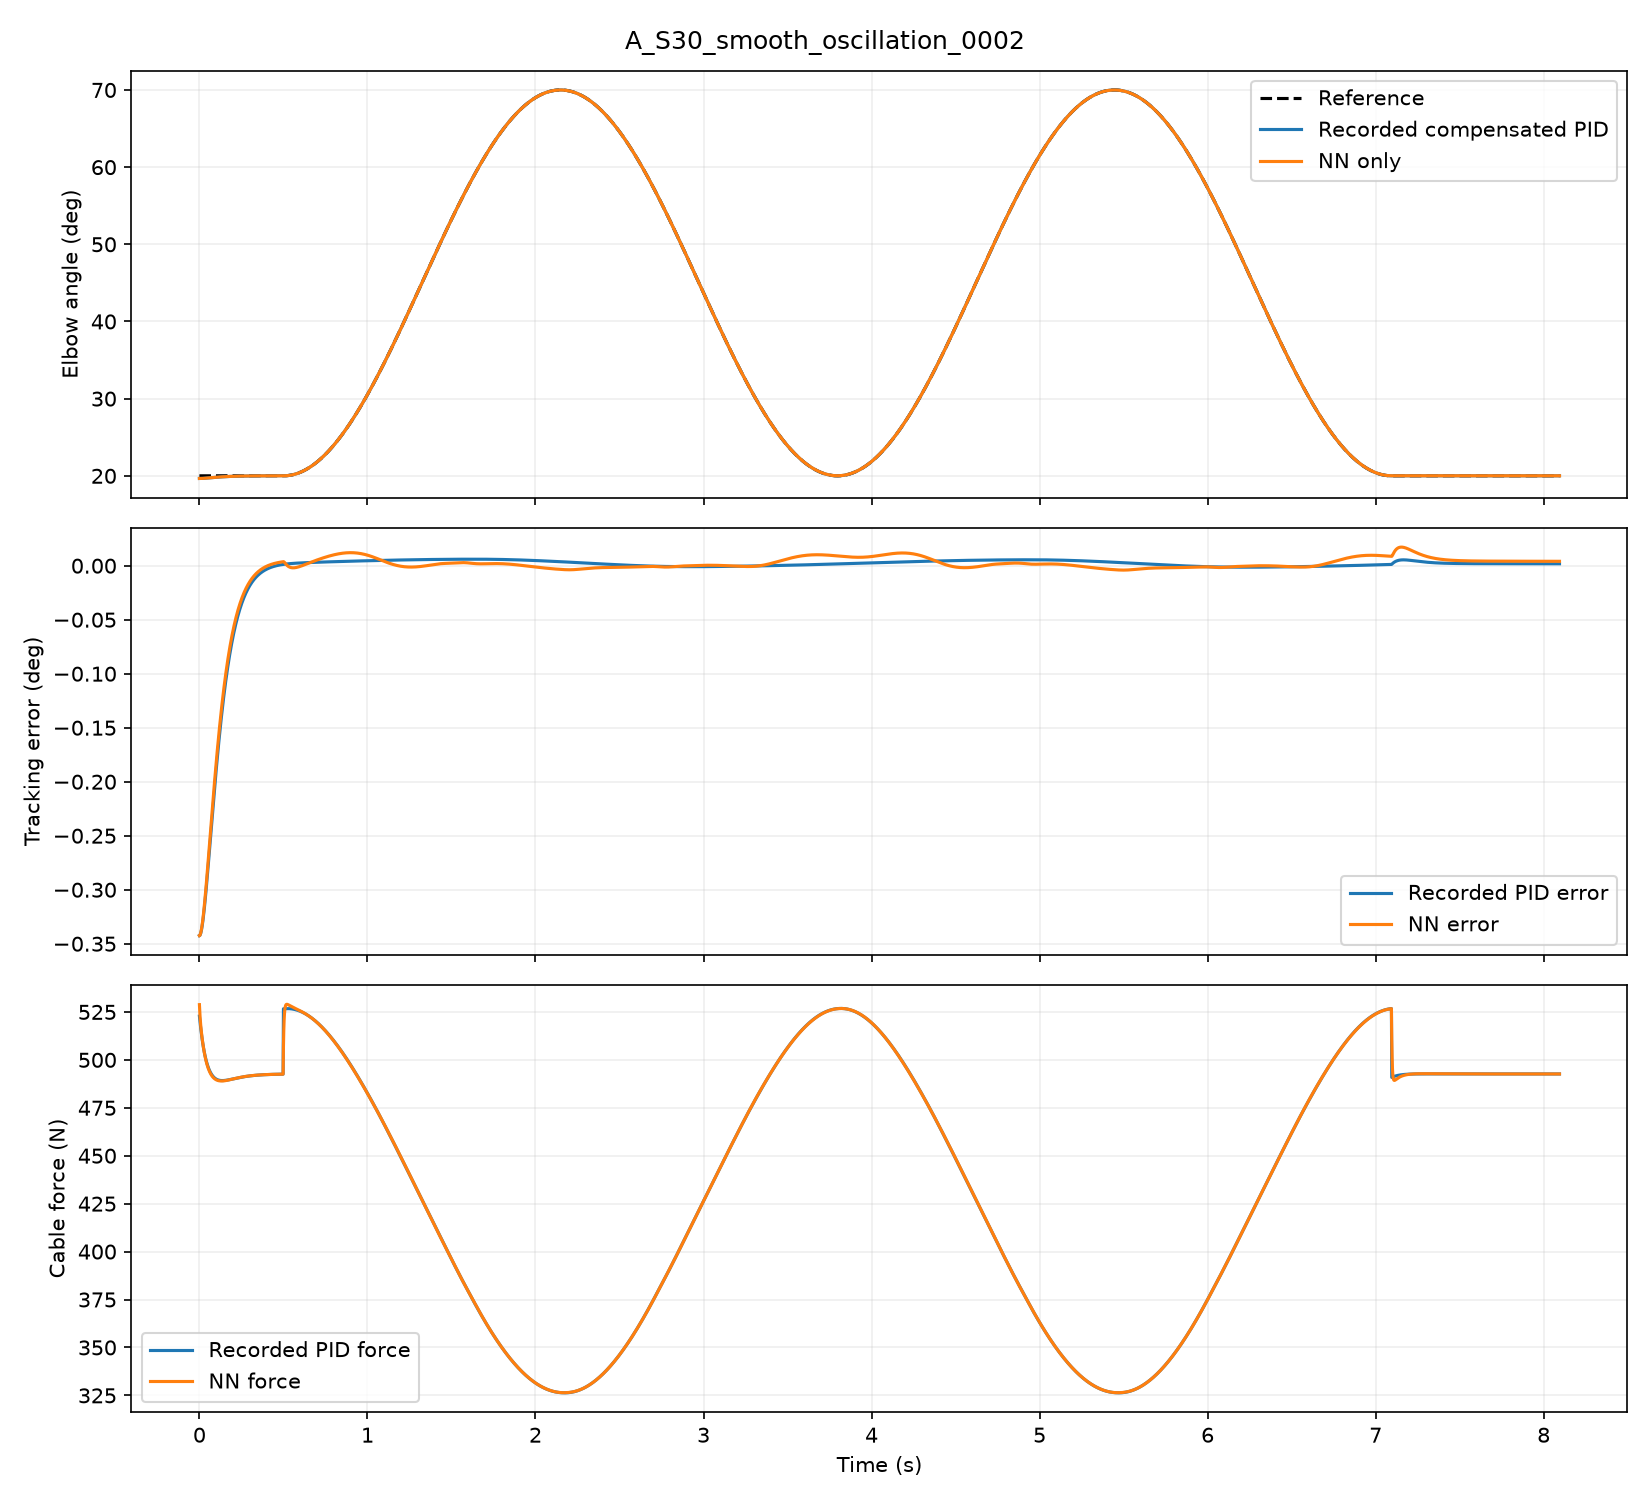
\includegraphics[width=\linewidth,height=0.69\textheight,keepaspectratio]{overleaf_figures/tracking_A_S30_smooth_oscillation_0002_comparison.png}
\caption{Example A\_S30\_smooth\_oscillation\_0002. Held-out OpenSim rollout: reference, recorded PID, and NN elbow motion; tracking errors; and cable forces. The NN supplies the cable command without a PID fallback.}
\label{fig:tracking_A_S30_smooth_oscillation_0002_comparison}
\end{figure}
\begin{figure}[H]\centering
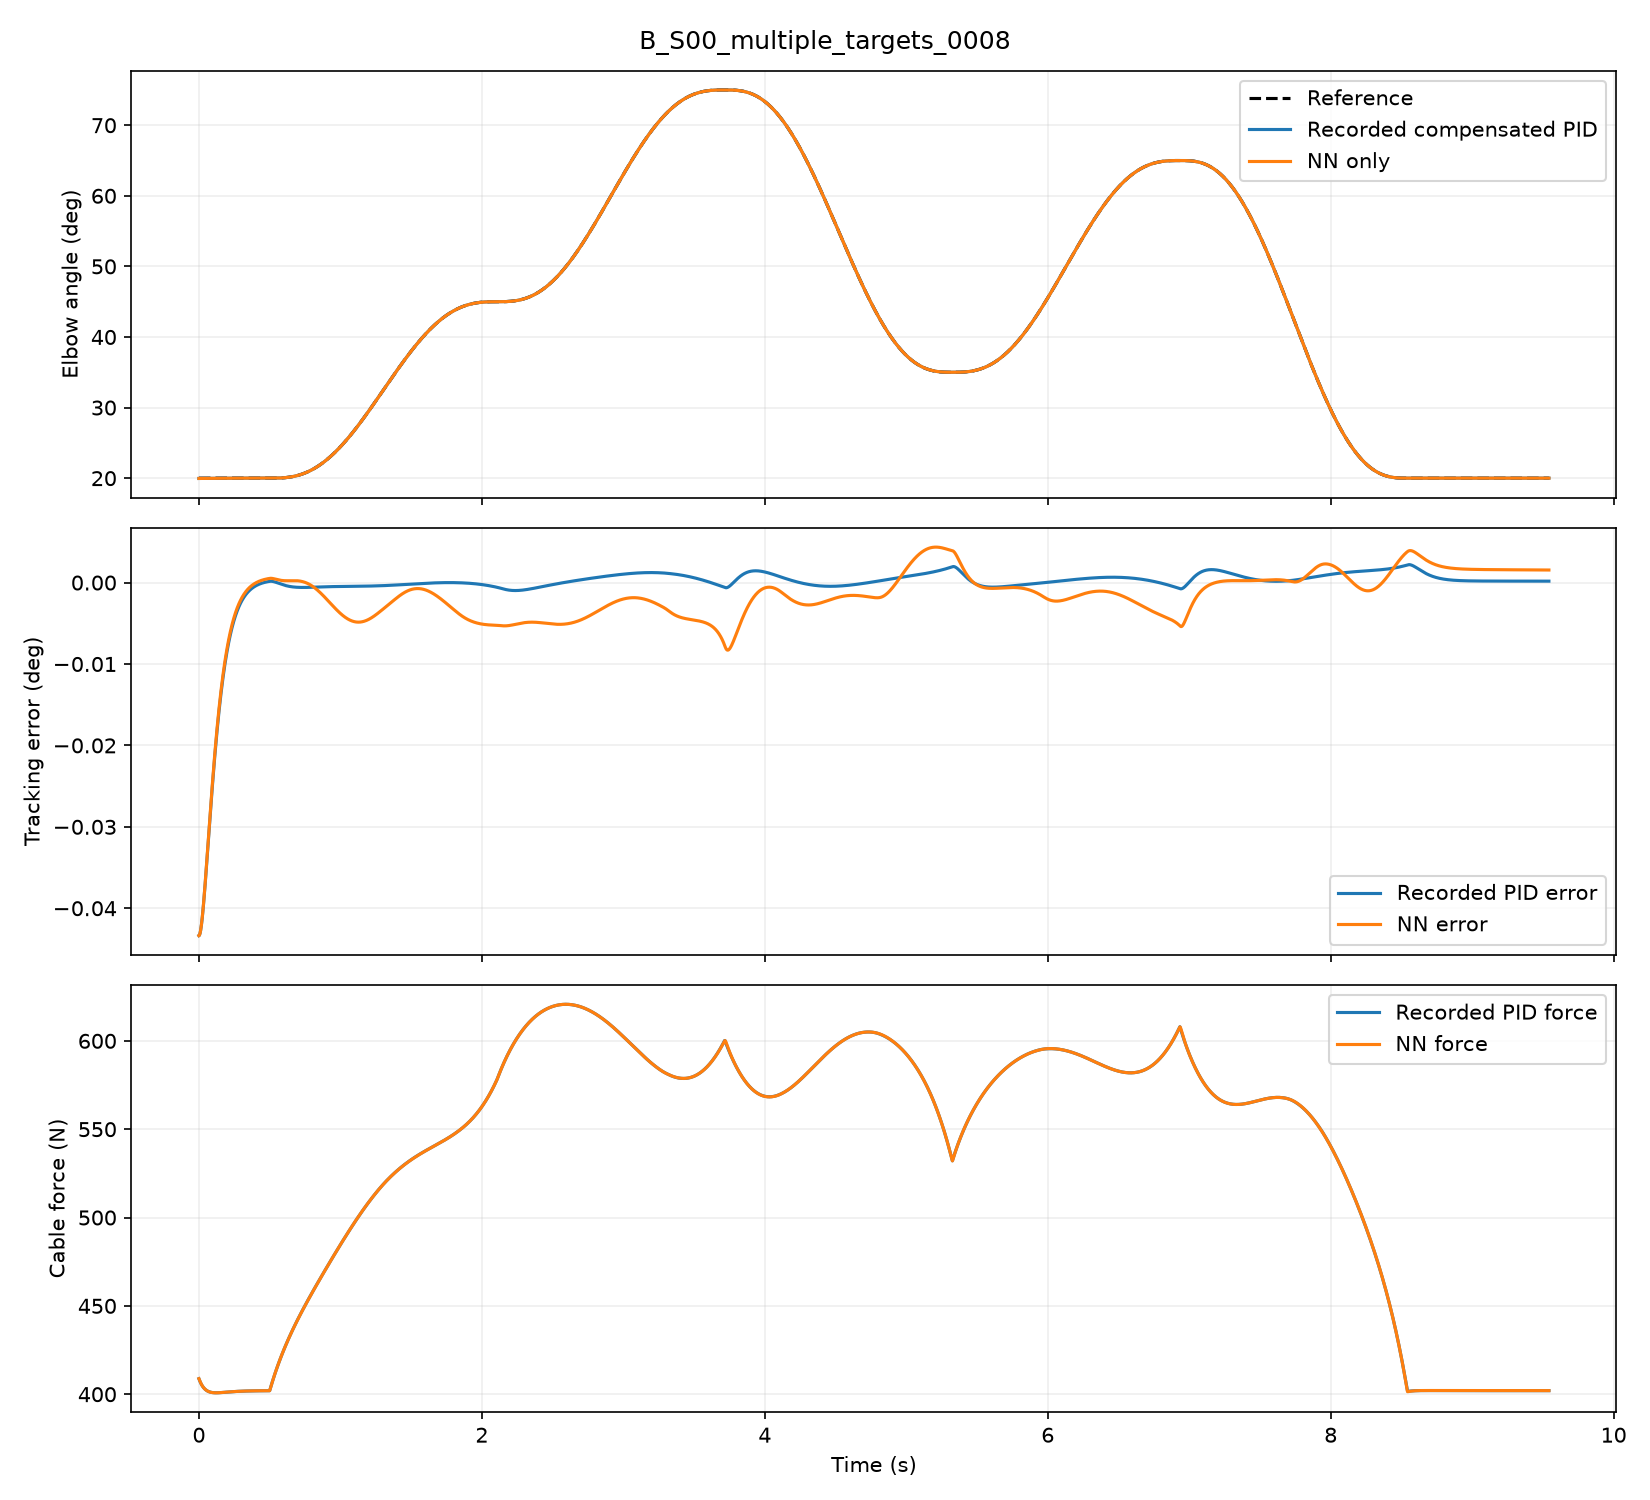
\includegraphics[width=\linewidth,height=0.69\textheight,keepaspectratio]{overleaf_figures/tracking_B_S00_multiple_targets_0008_comparison.png}
\caption{Example B\_S00\_multiple\_targets\_0008. Held-out OpenSim rollout: reference, recorded PID, and NN elbow motion; tracking errors; and cable forces. The NN supplies the cable command without a PID fallback.}
\label{fig:tracking_B_S00_multiple_targets_0008_comparison}
\end{figure}
\begin{figure}[H]\centering
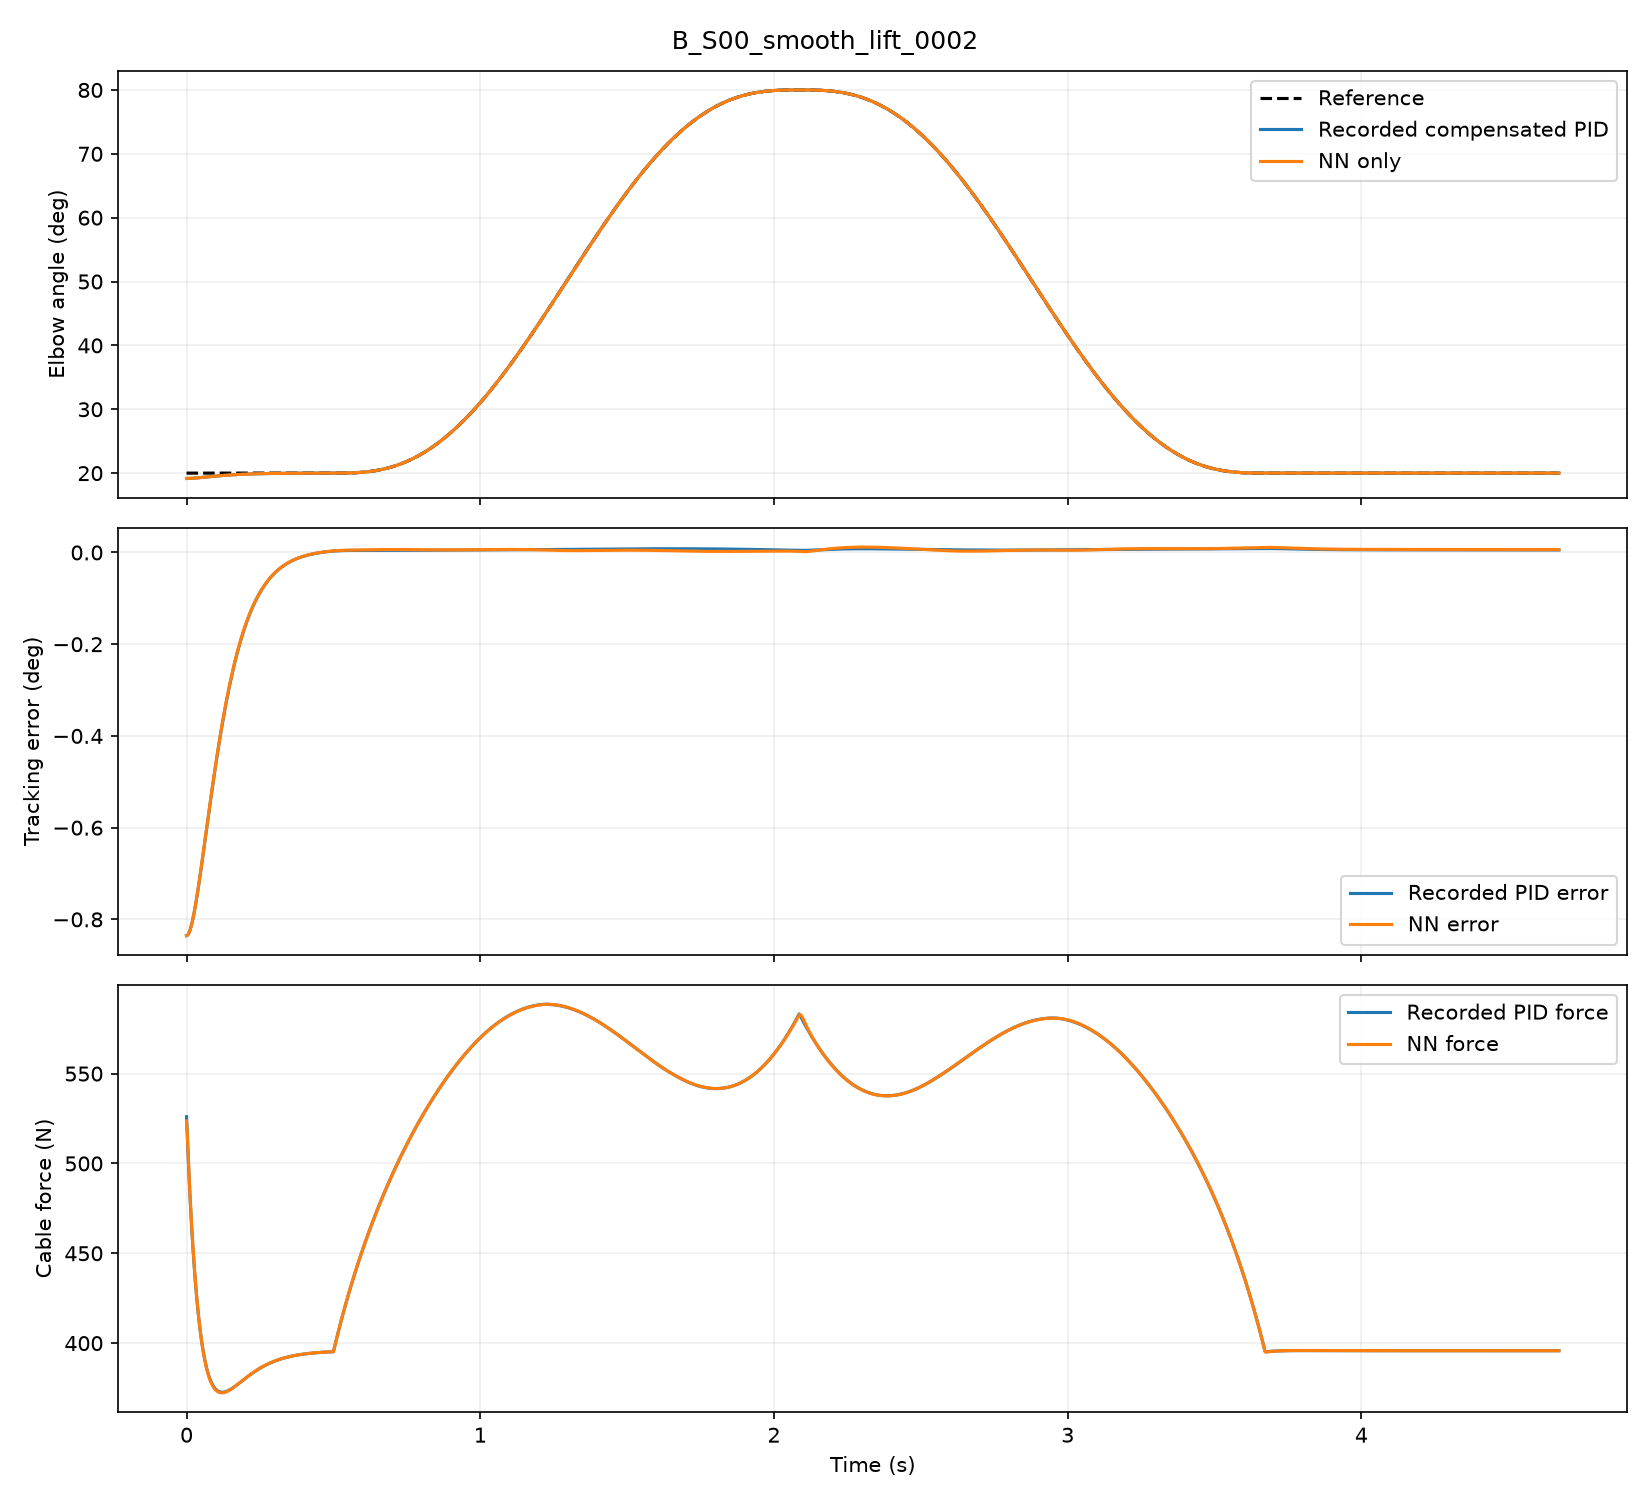
\includegraphics[width=\linewidth,height=0.69\textheight,keepaspectratio]{overleaf_figures/tracking_B_S00_smooth_lift_0002_comparison.png}
\caption{Example B\_S00\_smooth\_lift\_0002. Held-out OpenSim rollout: reference, recorded PID, and NN elbow motion; tracking errors; and cable forces. The NN supplies the cable command without a PID fallback.}
\label{fig:tracking_B_S00_smooth_lift_0002_comparison}
\end{figure}
\begin{figure}[H]\centering
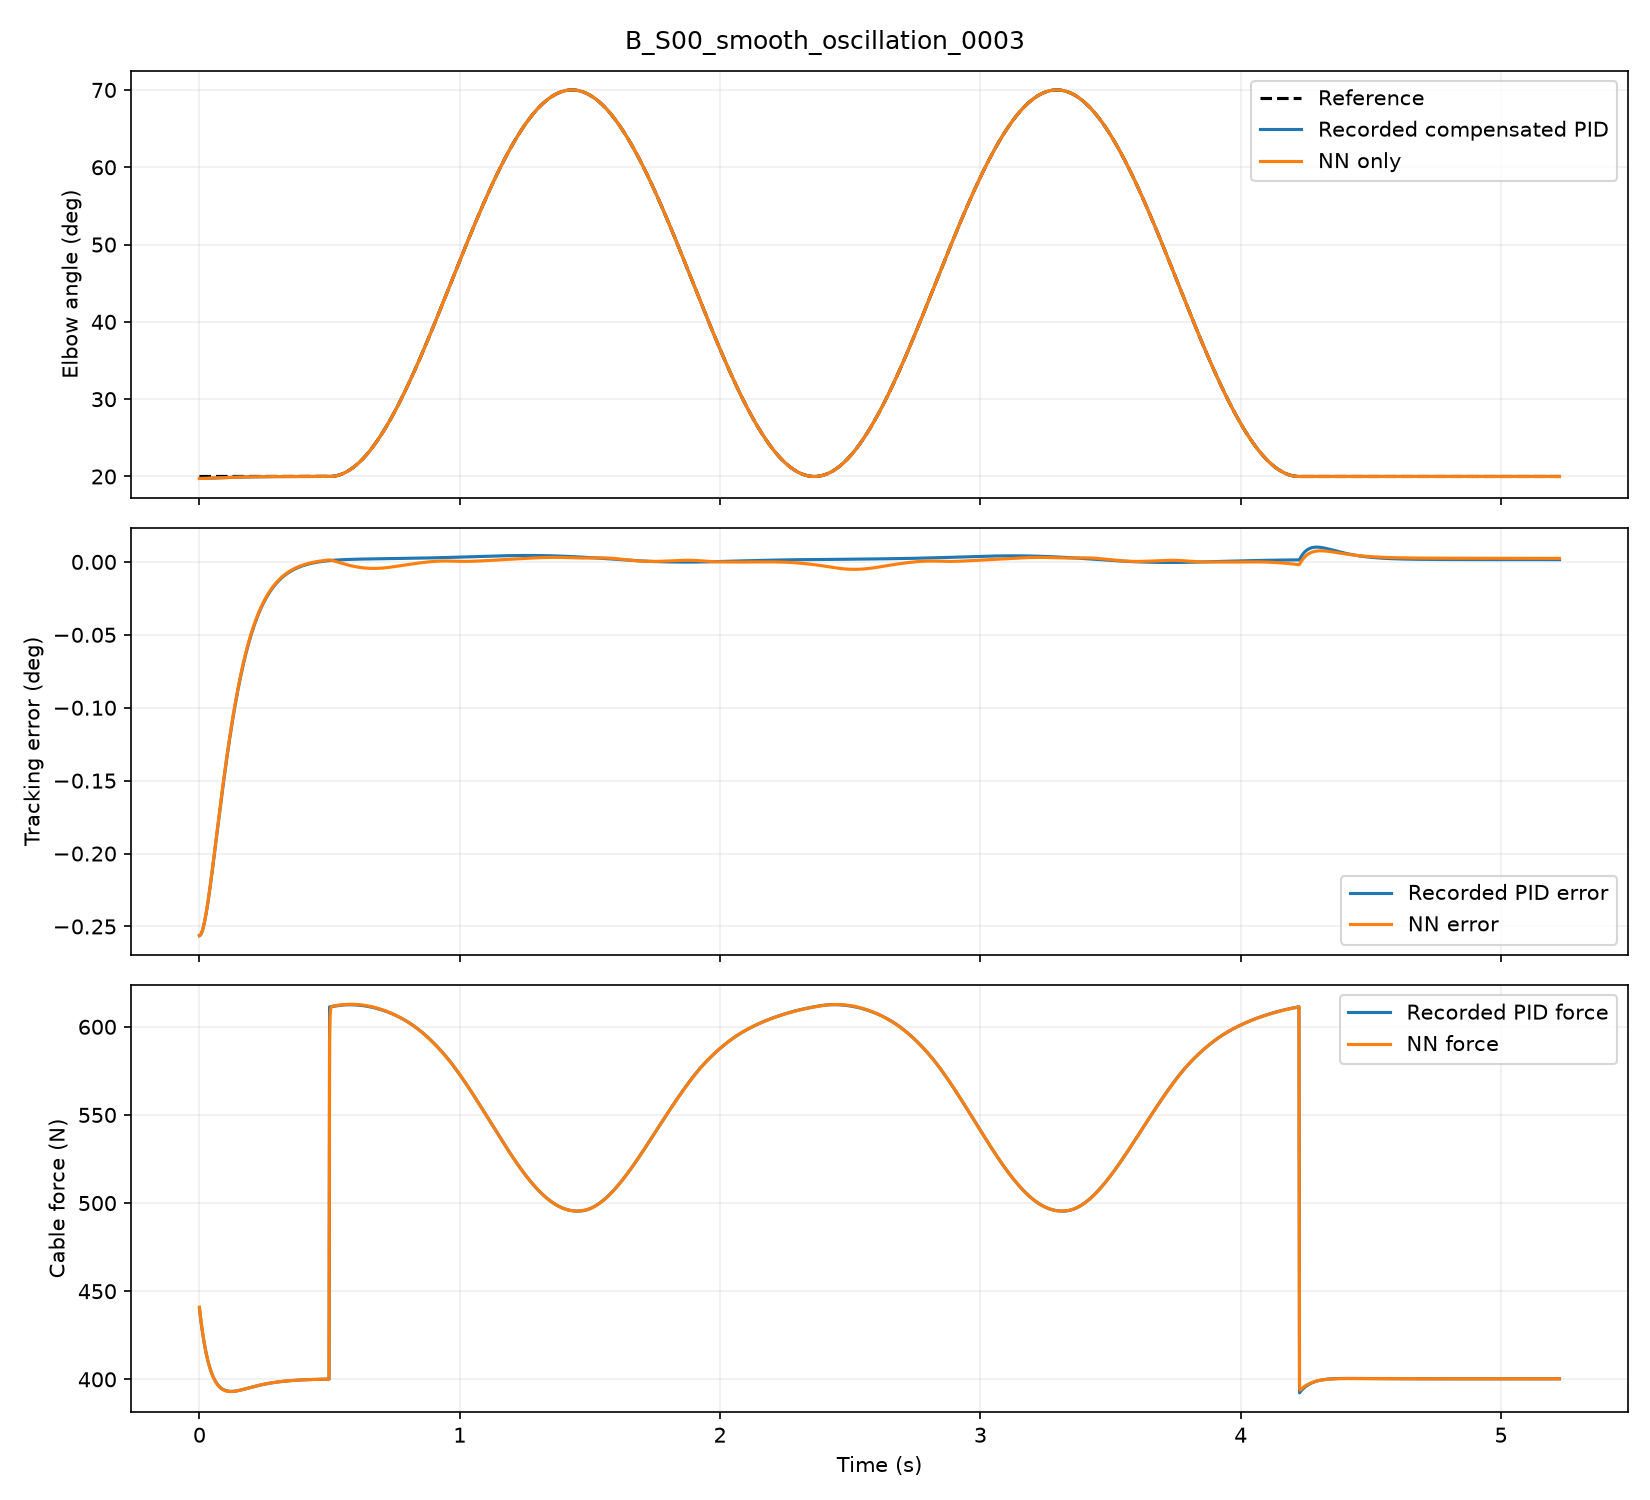
\includegraphics[width=\linewidth,height=0.69\textheight,keepaspectratio]{overleaf_figures/tracking_B_S00_smooth_oscillation_0003_comparison.png}
\caption{Example B\_S00\_smooth\_oscillation\_0003. Held-out OpenSim rollout: reference, recorded PID, and NN elbow motion; tracking errors; and cable forces. The NN supplies the cable command without a PID fallback.}
\label{fig:tracking_B_S00_smooth_oscillation_0003_comparison}
\end{figure}
\subsection*{Every attempted test episode}
\begin{longtable}{p{0.44\linewidth}rrrr}
\toprule Episode & PID RMSE & NN RMSE & NN max. & Pass\\\midrule\endhead
A\_S00\_multiple\_targets\_0006 & 0.0058838 & 0.0079034 & 0.87081 & Yes\\
A\_S00\_multiple\_targets\_0016 & 0.0055021 & 0.0056371 & 0.79827 & Yes\\
A\_S00\_multiple\_targets\_0018 & 0.0047692 & 0.0058955 & 0.69236 & Yes\\
A\_S00\_smooth\_lift\_0004 & 0.002493 & 0.0044048 & 0.30511 & Yes\\
A\_S00\_smooth\_lift\_0013 & 0.0010847 & 0.0090437 & 0.048156 & Yes\\
A\_S00\_smooth\_lift\_0014 & 0.0059916 & 0.0078851 & 0.77568 & Yes\\
A\_S00\_smooth\_oscillation\_0002 & 0.0058737 & 0.0077973 & 0.81574 & Yes\\
A\_S00\_smooth\_oscillation\_0004 & 0.0018054 & 0.0019457 & 0.22485 & Yes\\
A\_S00\_smooth\_oscillation\_0009 & 0.0065513 & 0.0096379 & 0.9075 & Yes\\
A\_S30\_multiple\_targets\_0002 & 0.0019712 & 0.0074725 & 0.045287 & Yes\\
A\_S30\_multiple\_targets\_0004 & 0.0032165 & 0.0070894 & 0.34044 & Yes\\
A\_S30\_multiple\_targets\_0016 & 0.0033239 & 0.0078976 & 0.40186 & Yes\\
A\_S30\_smooth\_lift\_0006 & 0.0053527 & 0.0095852 & 0.61319 & Yes\\
A\_S30\_smooth\_lift\_0009 & 0.0036545 & 0.0061702 & 0.32992 & Yes\\
A\_S30\_smooth\_lift\_0013 & 0.0059796 & 0.0076568 & 0.74139 & Yes\\
A\_S30\_smooth\_oscillation\_0002 & 0.0034094 & 0.0048669 & 0.3425 & Yes\\
A\_S30\_smooth\_oscillation\_0017 & 0.0070303 & 0.0082037 & 0.94228 & Yes\\
A\_S30\_smooth\_oscillation\_0019 & 0.0072336 & 0.006592 & 0.92856 & Yes\\
B\_S00\_multiple\_targets\_0008 & 0.00077796 & 0.0029919 & 0.043366 & Yes\\
B\_S00\_multiple\_targets\_0010 & 0.0056578 & 0.0077391 & 0.81114 & Yes\\
B\_S00\_multiple\_targets\_0018 & 0.0013208 & 0.0022642 & 0.16156 & Yes\\
B\_S00\_smooth\_lift\_0002 & 0.006575 & 0.0063781 & 0.83545 & Yes\\
B\_S00\_smooth\_lift\_0006 & 0.003066 & 0.0036979 & 0.34369 & Yes\\
B\_S00\_smooth\_lift\_0011 & 0.0025075 & 0.004199 & 0.24894 & Yes\\
B\_S00\_smooth\_oscillation\_0003 & 0.0024325 & 0.0020345 & 0.25628 & Yes\\
B\_S00\_smooth\_oscillation\_0013 & 0.0011009 & 0.0011667 & 0.033751 & Yes\\
B\_S00\_smooth\_oscillation\_0018 & 0.0030237 & 0.0030936 & 0.37132 & Yes\\
\bottomrule\end{longtable}
All errors in the table are degrees. The full saved trajectories and command histories remain in the original results folder.
\section*{4. Duration and sampling check}
The export inspected signals from 27 attempted episodes. Positive, increasing recorded time was found in 27 episodes. The accompanying sampling audit lists every sample count, time span, median interval, configured interval, and recorded computation time.
Runtime alone is not evidence of correctness. The sampling audit reports recorded values; it does not independently prove that every configured final time was reached.
\begin{figure}[H]\centering
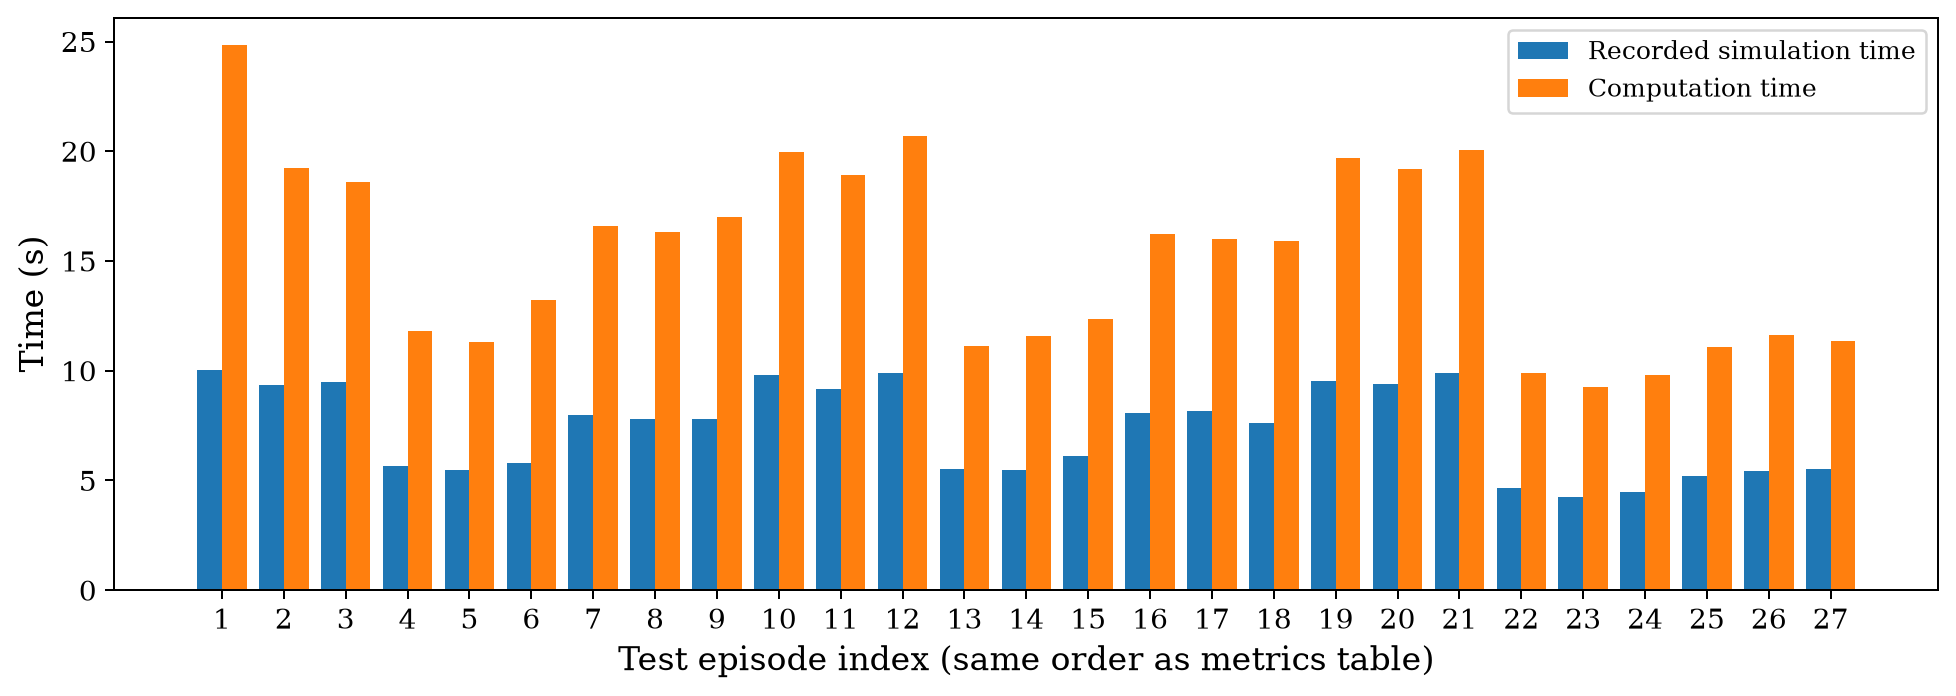
\includegraphics[width=\linewidth,height=0.69\textheight,keepaspectratio]{overleaf_figures/duration_audit.png}
\caption{Recorded simulation duration and computation time for each episode. Simulation time and wall-clock time are different quantities.}
\label{fig:duration_audit}
\end{figure}
\section*{Scope of the conclusion}
The evidence supports performance on held-out episodes within the collected trajectory families and feasible configurations. It does not establish arbitrary new-trajectory generalization, real-world performance, or superiority over PID. A single training seed is not a repeated-seed robustness study. States outside training feature ranges are reported in the original comparison file.
Run status: completed. Report creation alone is not a success criterion.
\clearpage\appendix\section*{Appendix: complete saved figure set}
Every remaining saved PNG is included below, with a short explanation. This appendix retains all episode diagnostics; the main text presents learning curves, test force accuracy, and tracking evidence.
\begin{figure}[H]\centering
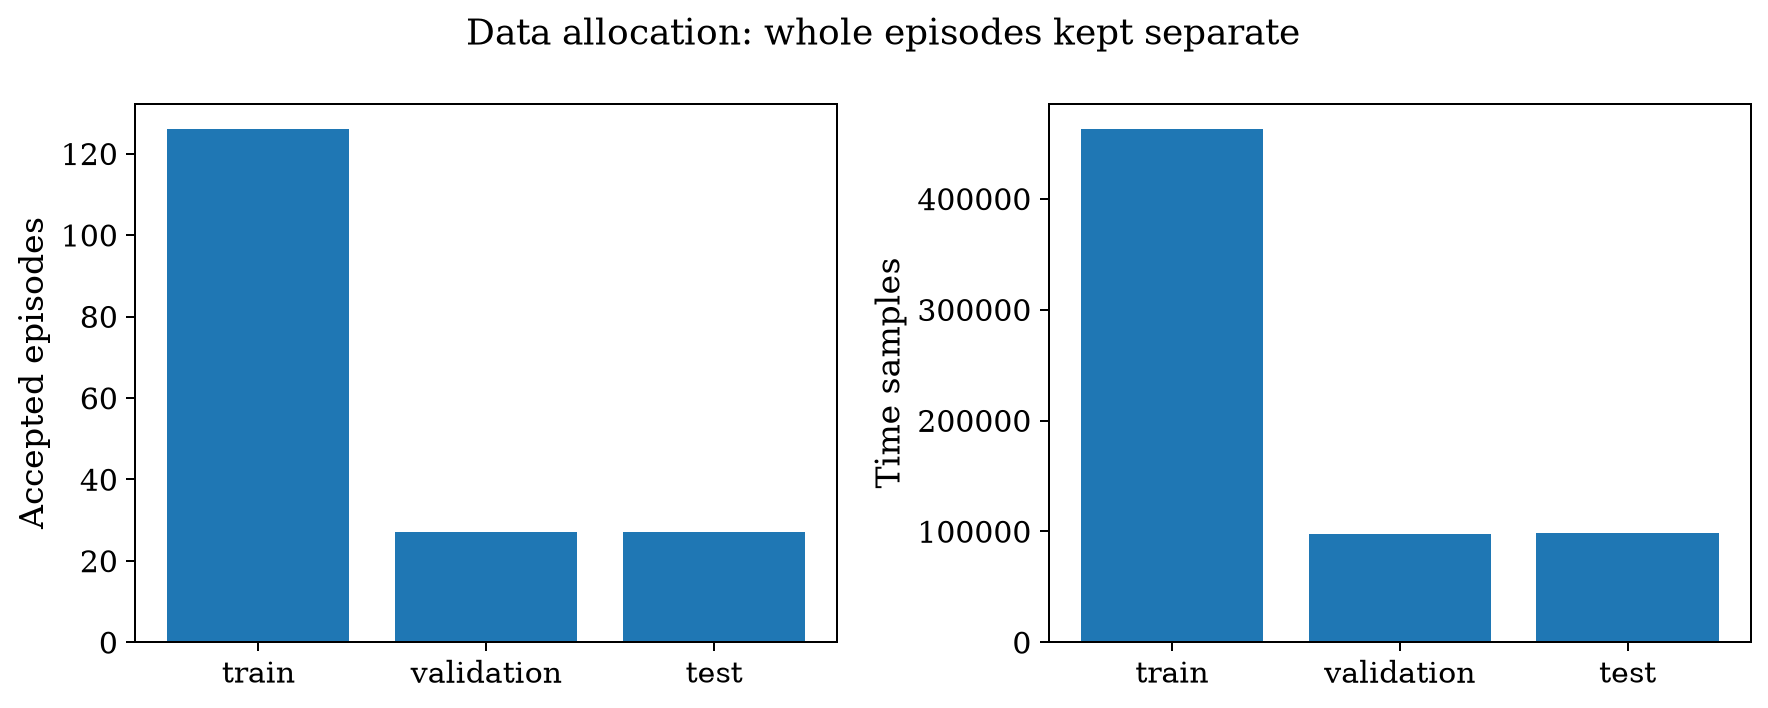
\includegraphics[width=\linewidth,height=0.69\textheight,keepaspectratio]{overleaf_figures/data_split.png}
\caption{data\_split.png: Actual accepted episode and sample counts. Whole episodes remain in their original split.}
\label{fig:data_split}
\end{figure}
\begin{figure}[H]\centering
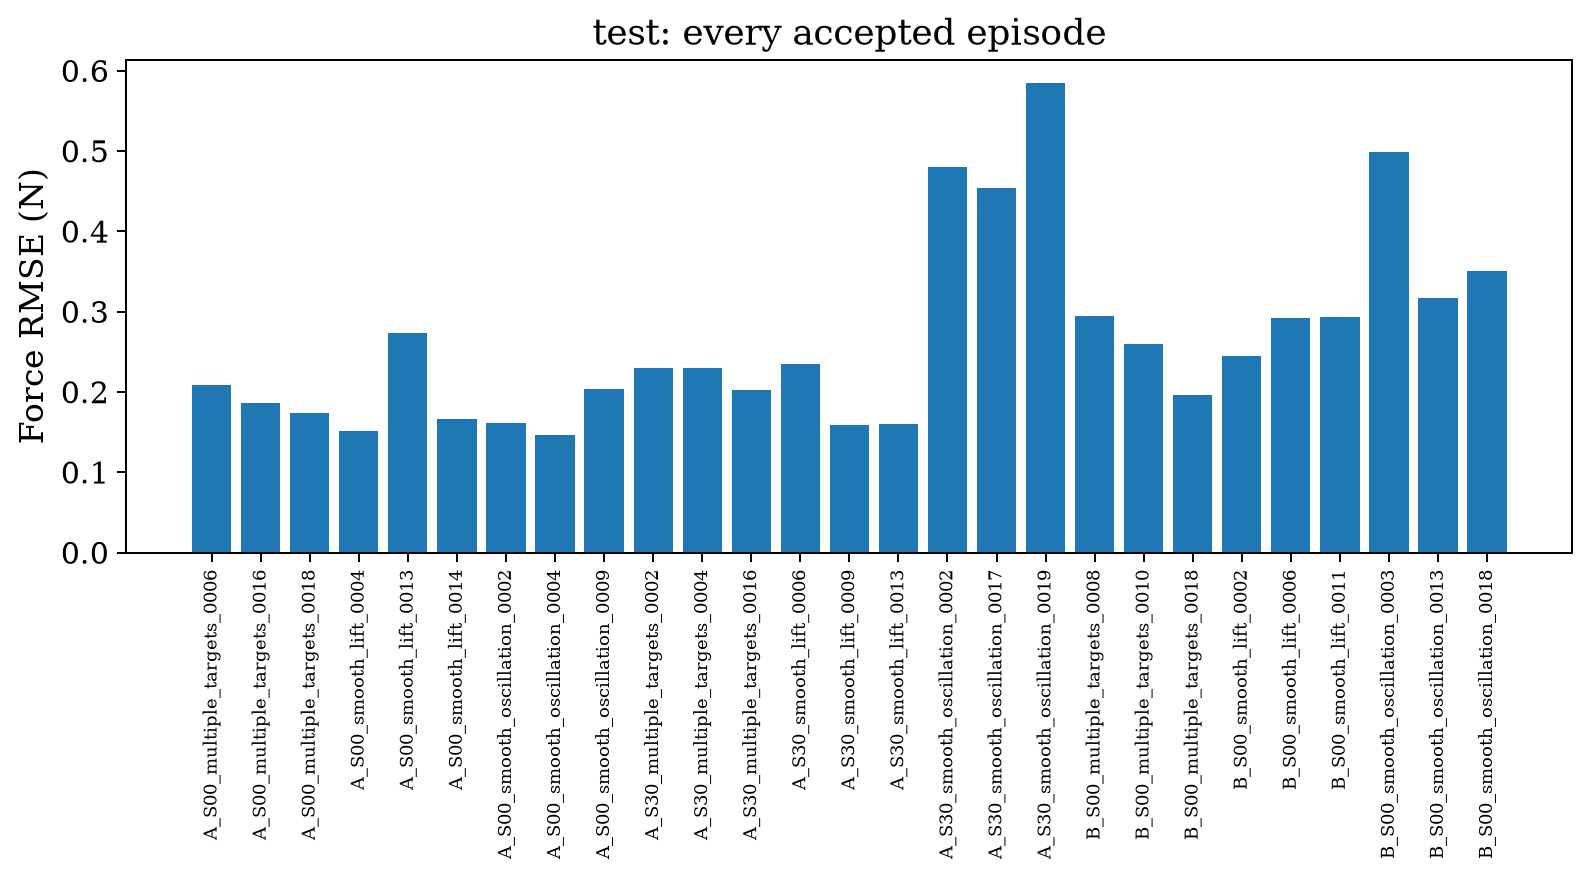
\includegraphics[width=\linewidth,height=0.69\textheight,keepaspectratio]{overleaf_figures/test_episode_errors.png}
\caption{test\_episode\_errors.png: Force RMSE for every included episode in this split. Large episode-specific errors remain visible.}
\label{fig:test_episode_errors}
\end{figure}
\begin{figure}[H]\centering
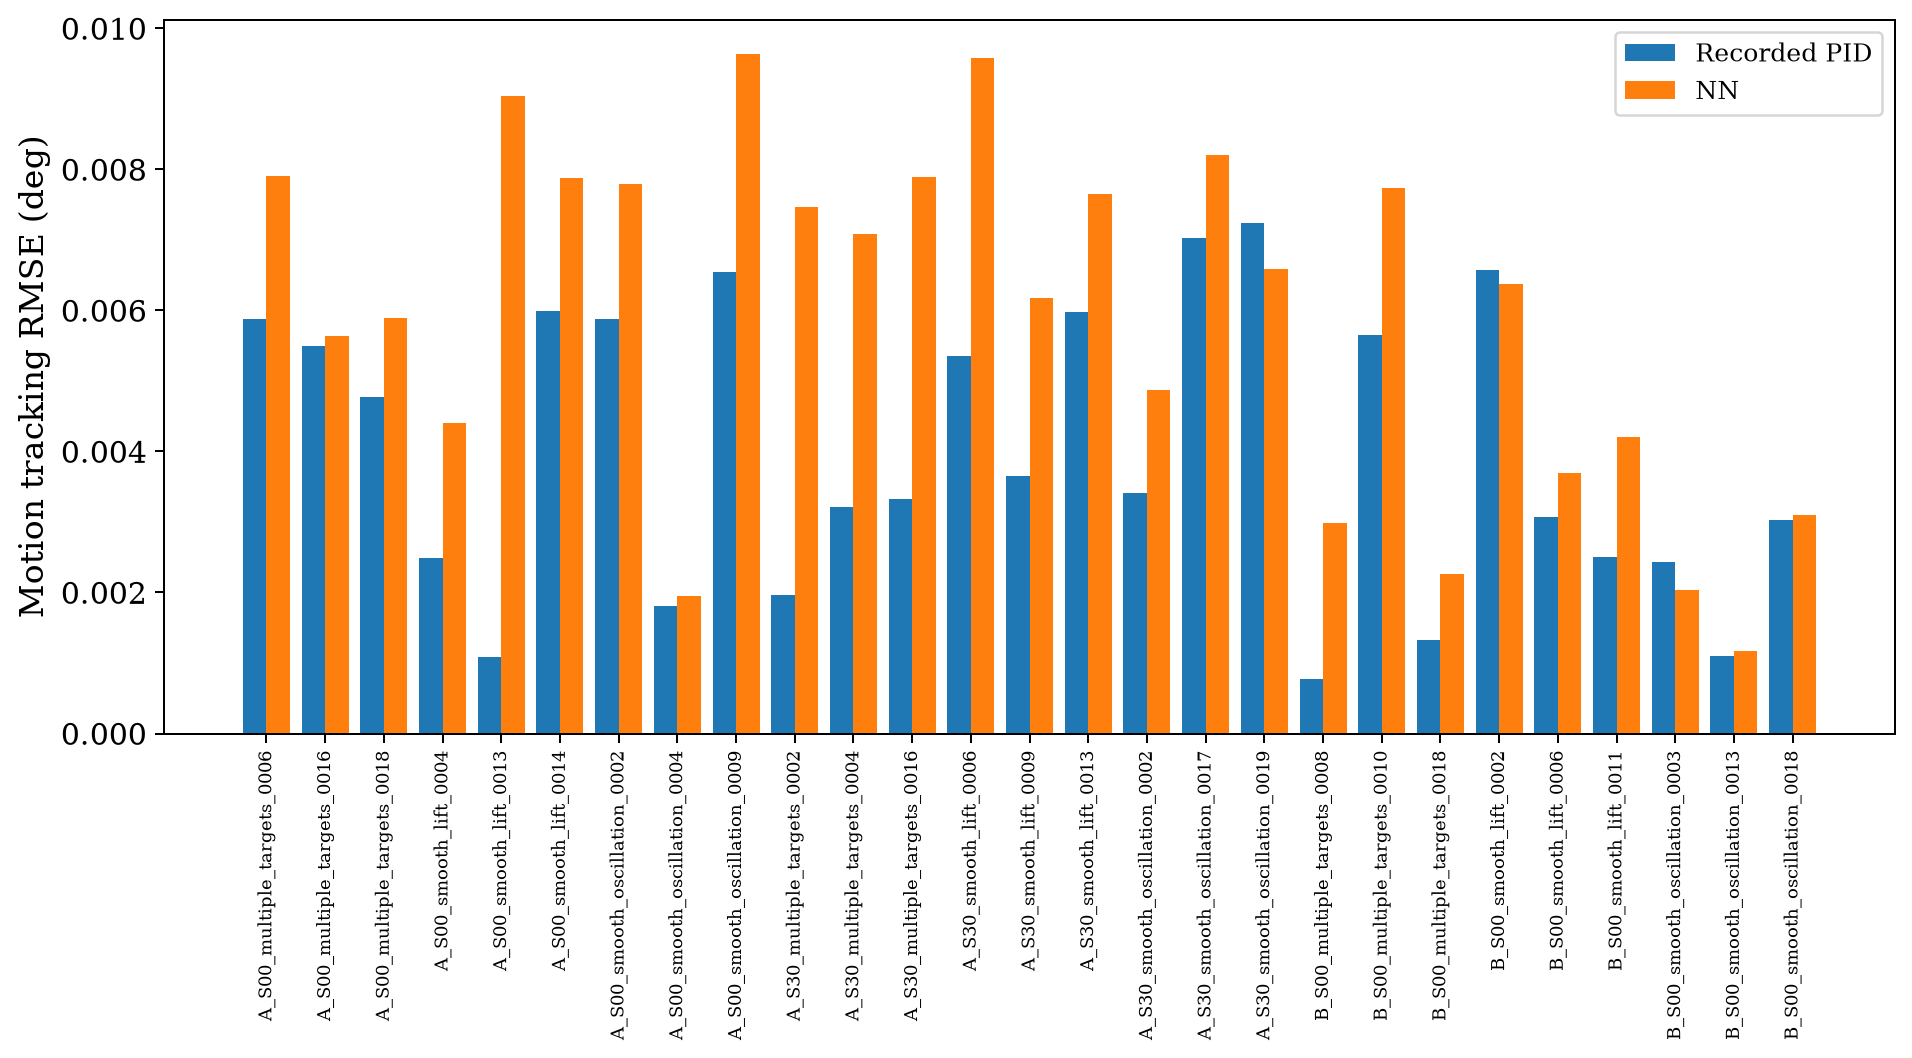
\includegraphics[width=\linewidth,height=0.69\textheight,keepaspectratio]{overleaf_figures/tracking_summary.png}
\caption{tracking\_summary.png: Tracking accuracy across every evaluated episode. Motion RMSE excludes the configured holds; maximum error covers the complete recorded episode.}
\label{fig:tracking_summary}
\end{figure}
\begin{figure}[H]\centering
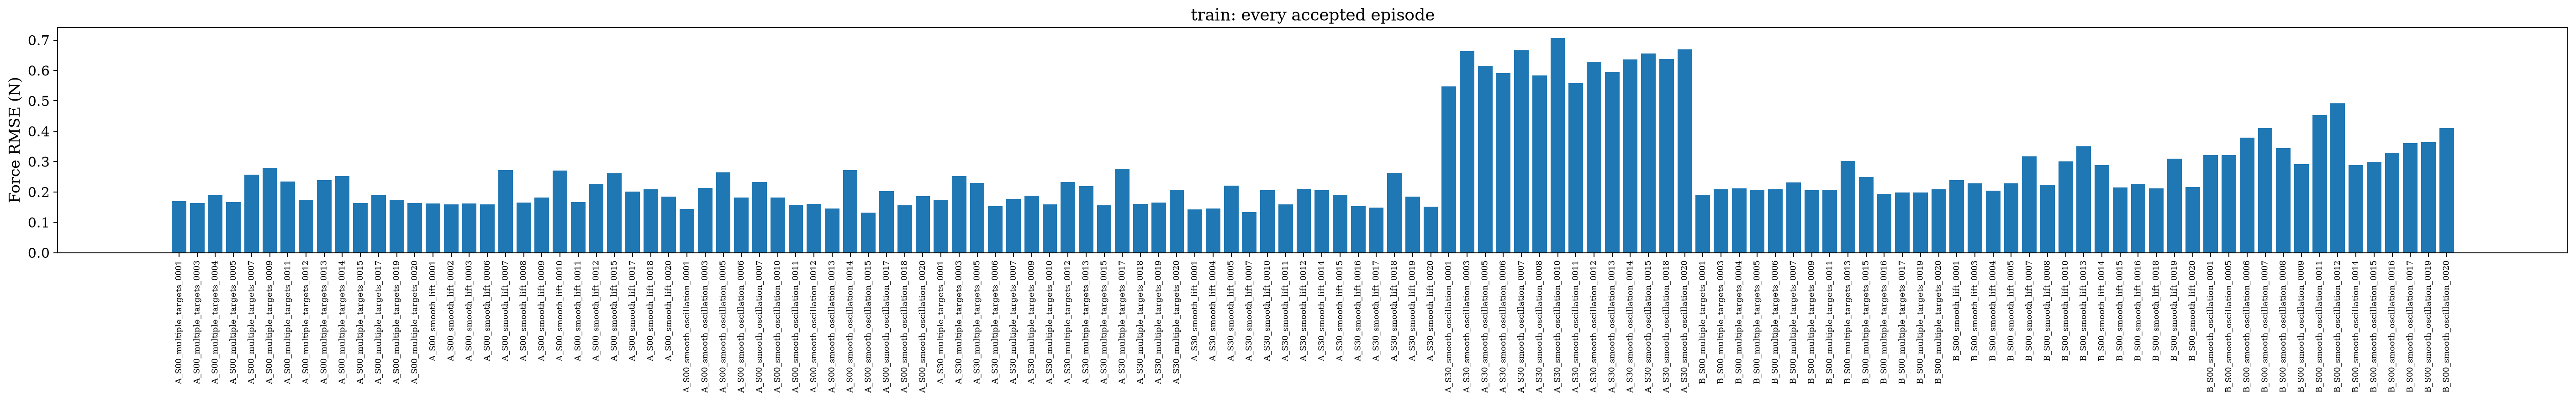
\includegraphics[width=\linewidth,height=0.69\textheight,keepaspectratio]{overleaf_figures/train_episode_errors.png}
\caption{train\_episode\_errors.png: Force RMSE for every included episode in this split. Large episode-specific errors remain visible.}
\label{fig:train_episode_errors}
\end{figure}
\begin{figure}[H]\centering
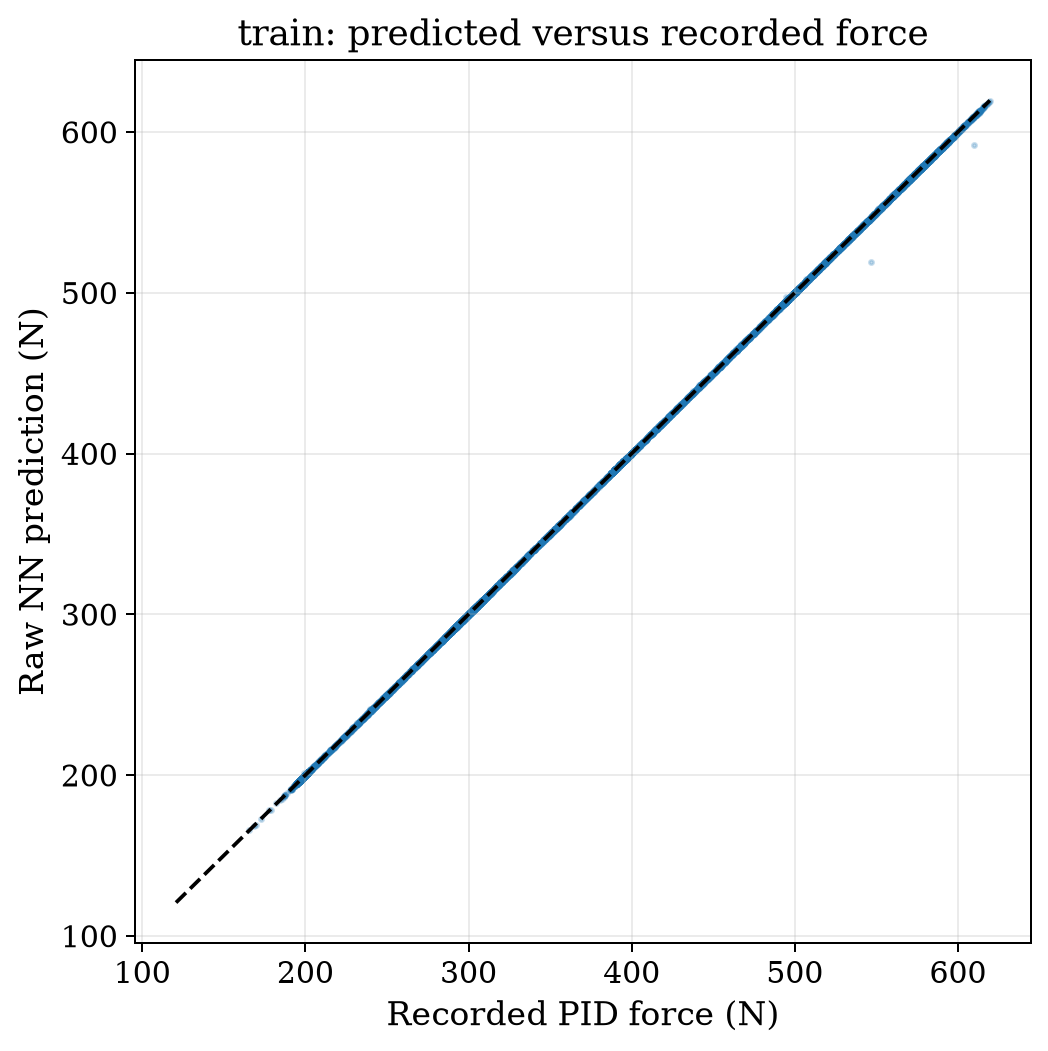
\includegraphics[width=\linewidth,height=0.69\textheight,keepaspectratio]{overleaf_figures/train_parity.png}
\caption{train\_parity.png: Predicted versus recorded compensated-PID force. Agreement with the diagonal indicates accurate force imitation; it does not by itself establish closed-loop tracking.}
\label{fig:train_parity}
\end{figure}
\begin{figure}[H]\centering
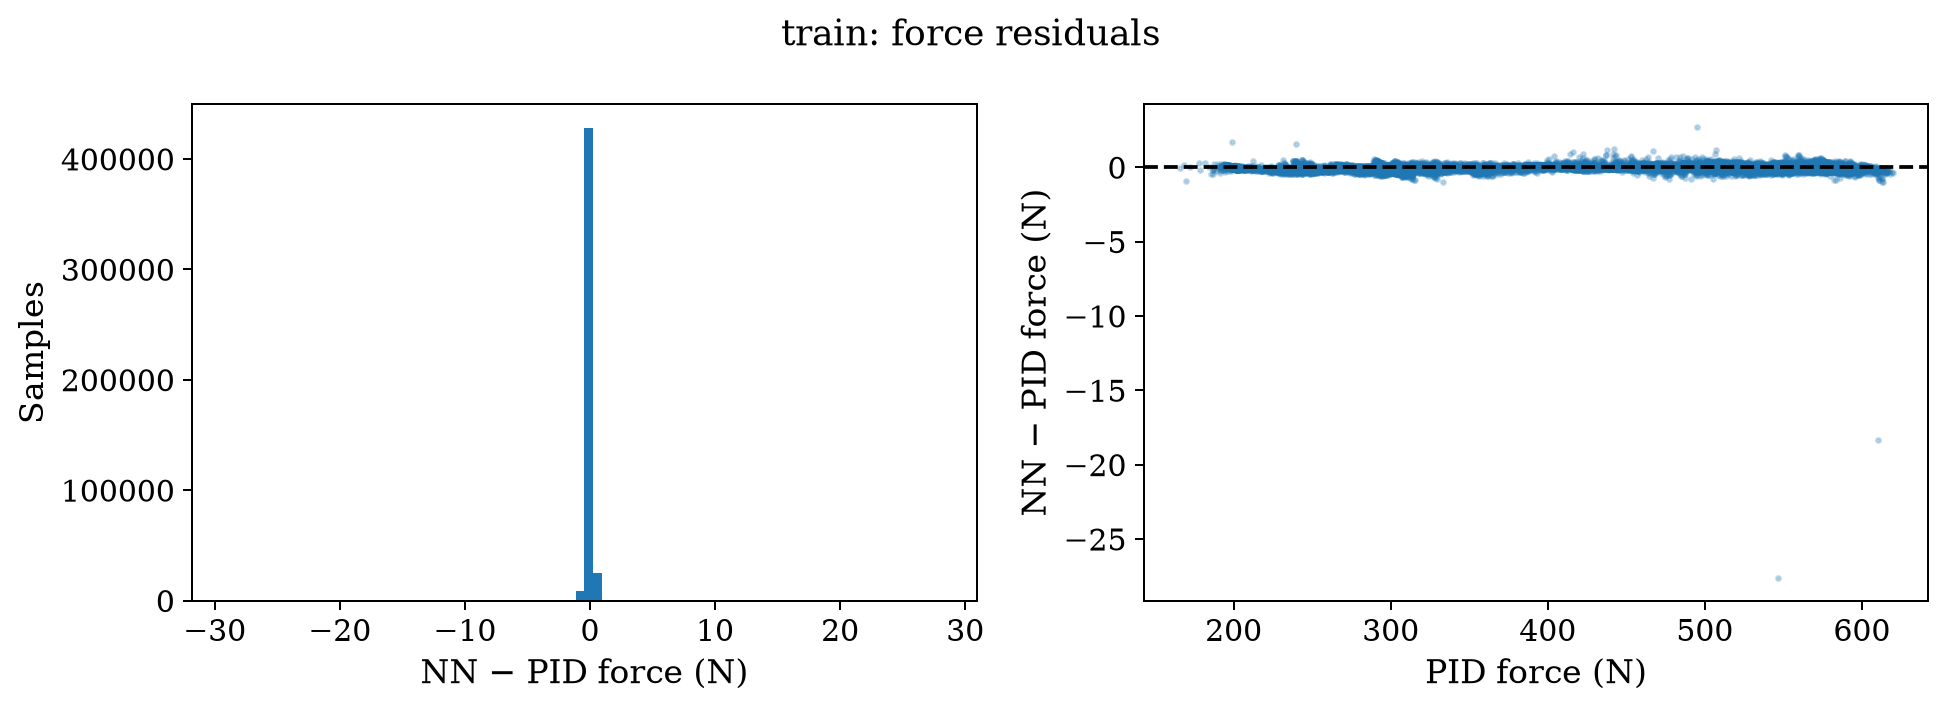
\includegraphics[width=\linewidth,height=0.69\textheight,keepaspectratio]{overleaf_figures/train_residuals.png}
\caption{train\_residuals.png: Force residuals (NN minus recorded PID). The distribution and force-dependent scatter expose bias and large errors.}
\label{fig:train_residuals}
\end{figure}
\begin{figure}[H]\centering
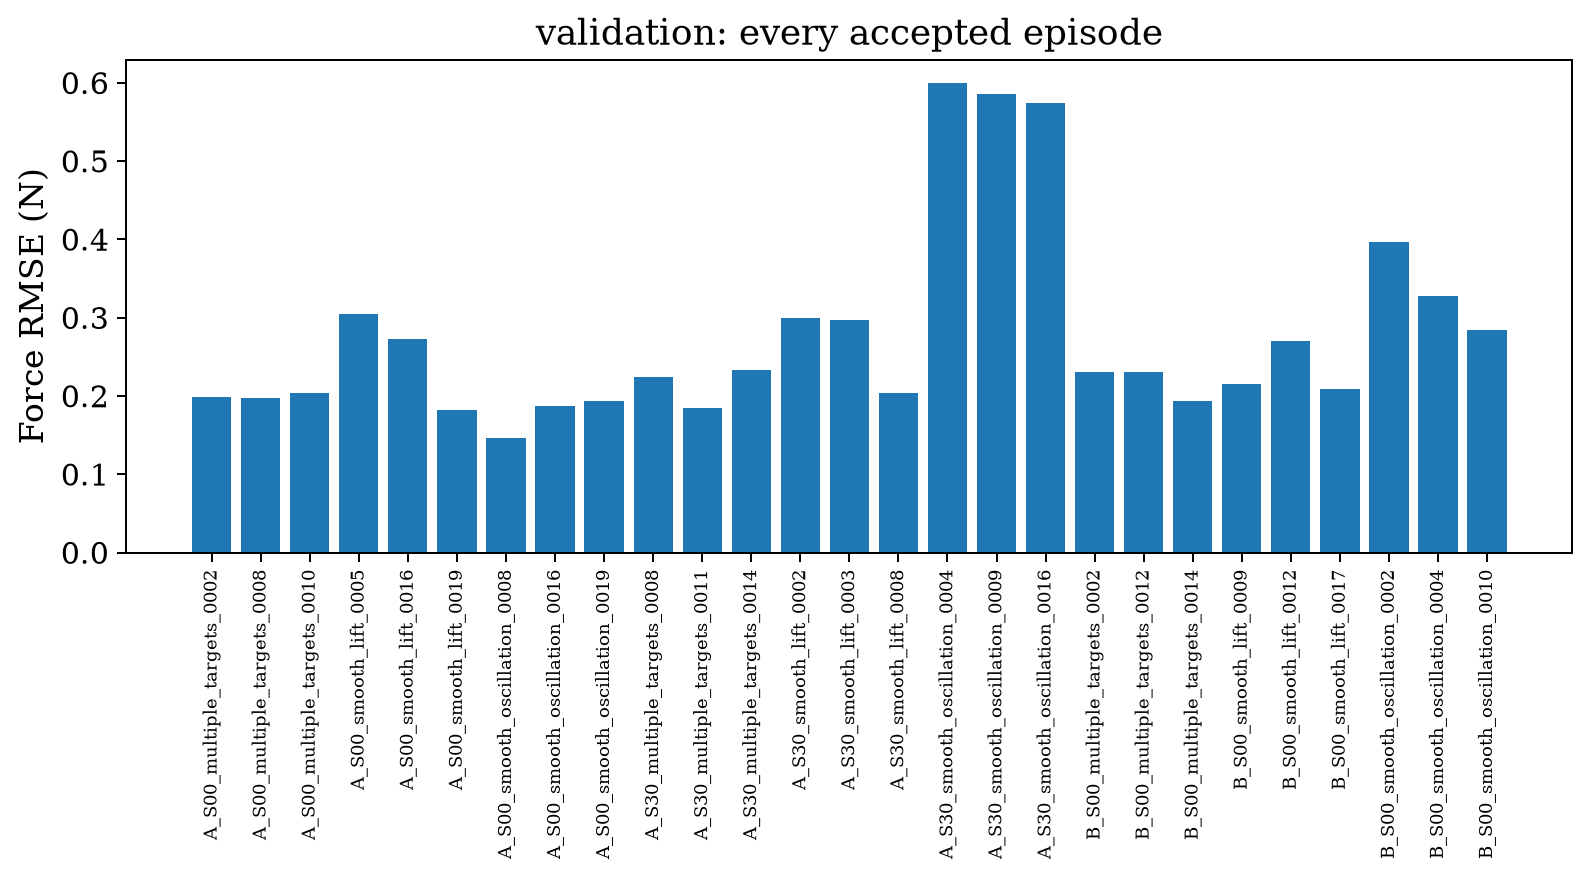
\includegraphics[width=\linewidth,height=0.69\textheight,keepaspectratio]{overleaf_figures/validation_episode_errors.png}
\caption{validation\_episode\_errors.png: Force RMSE for every included episode in this split. Large episode-specific errors remain visible.}
\label{fig:validation_episode_errors}
\end{figure}
\begin{figure}[H]\centering
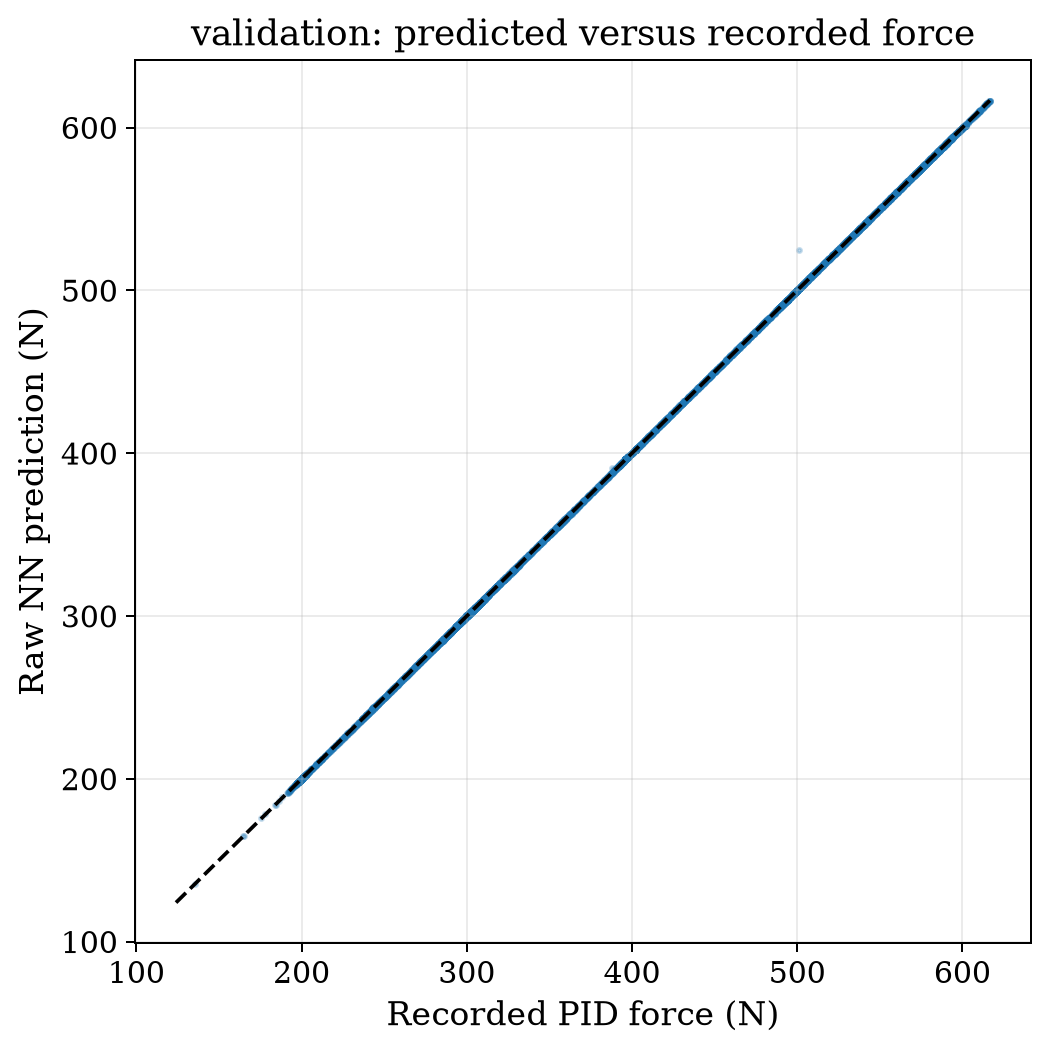
\includegraphics[width=\linewidth,height=0.69\textheight,keepaspectratio]{overleaf_figures/validation_parity.png}
\caption{validation\_parity.png: Predicted versus recorded compensated-PID force. Agreement with the diagonal indicates accurate force imitation; it does not by itself establish closed-loop tracking.}
\label{fig:validation_parity}
\end{figure}
\begin{figure}[H]\centering
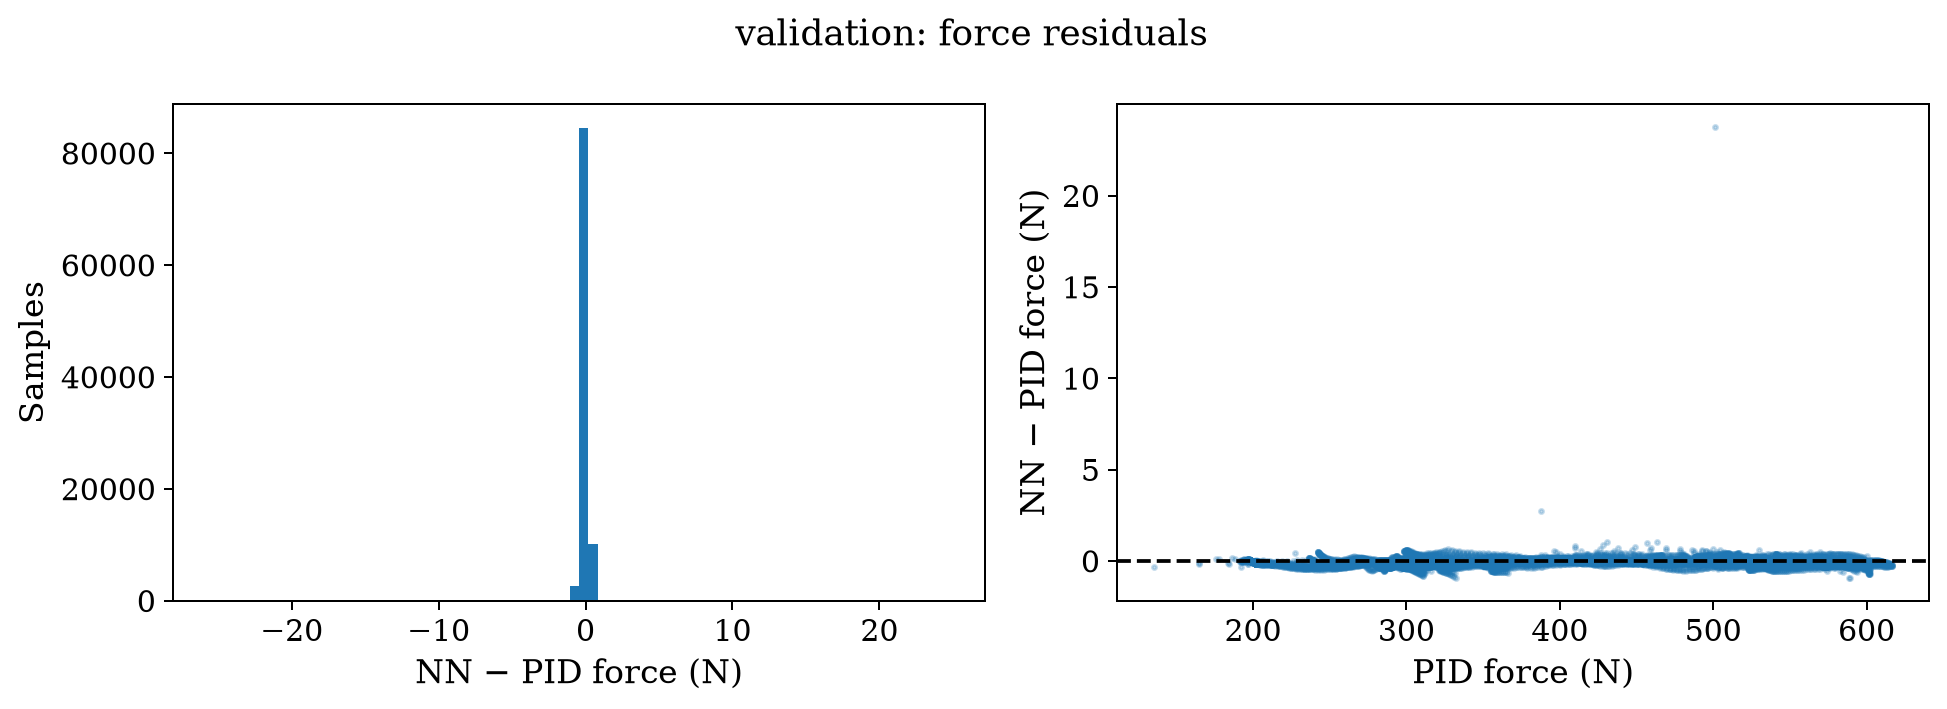
\includegraphics[width=\linewidth,height=0.69\textheight,keepaspectratio]{overleaf_figures/validation_residuals.png}
\caption{validation\_residuals.png: Force residuals (NN minus recorded PID). The distribution and force-dependent scatter expose bias and large errors.}
\label{fig:validation_residuals}
\end{figure}
\begin{figure}[H]\centering
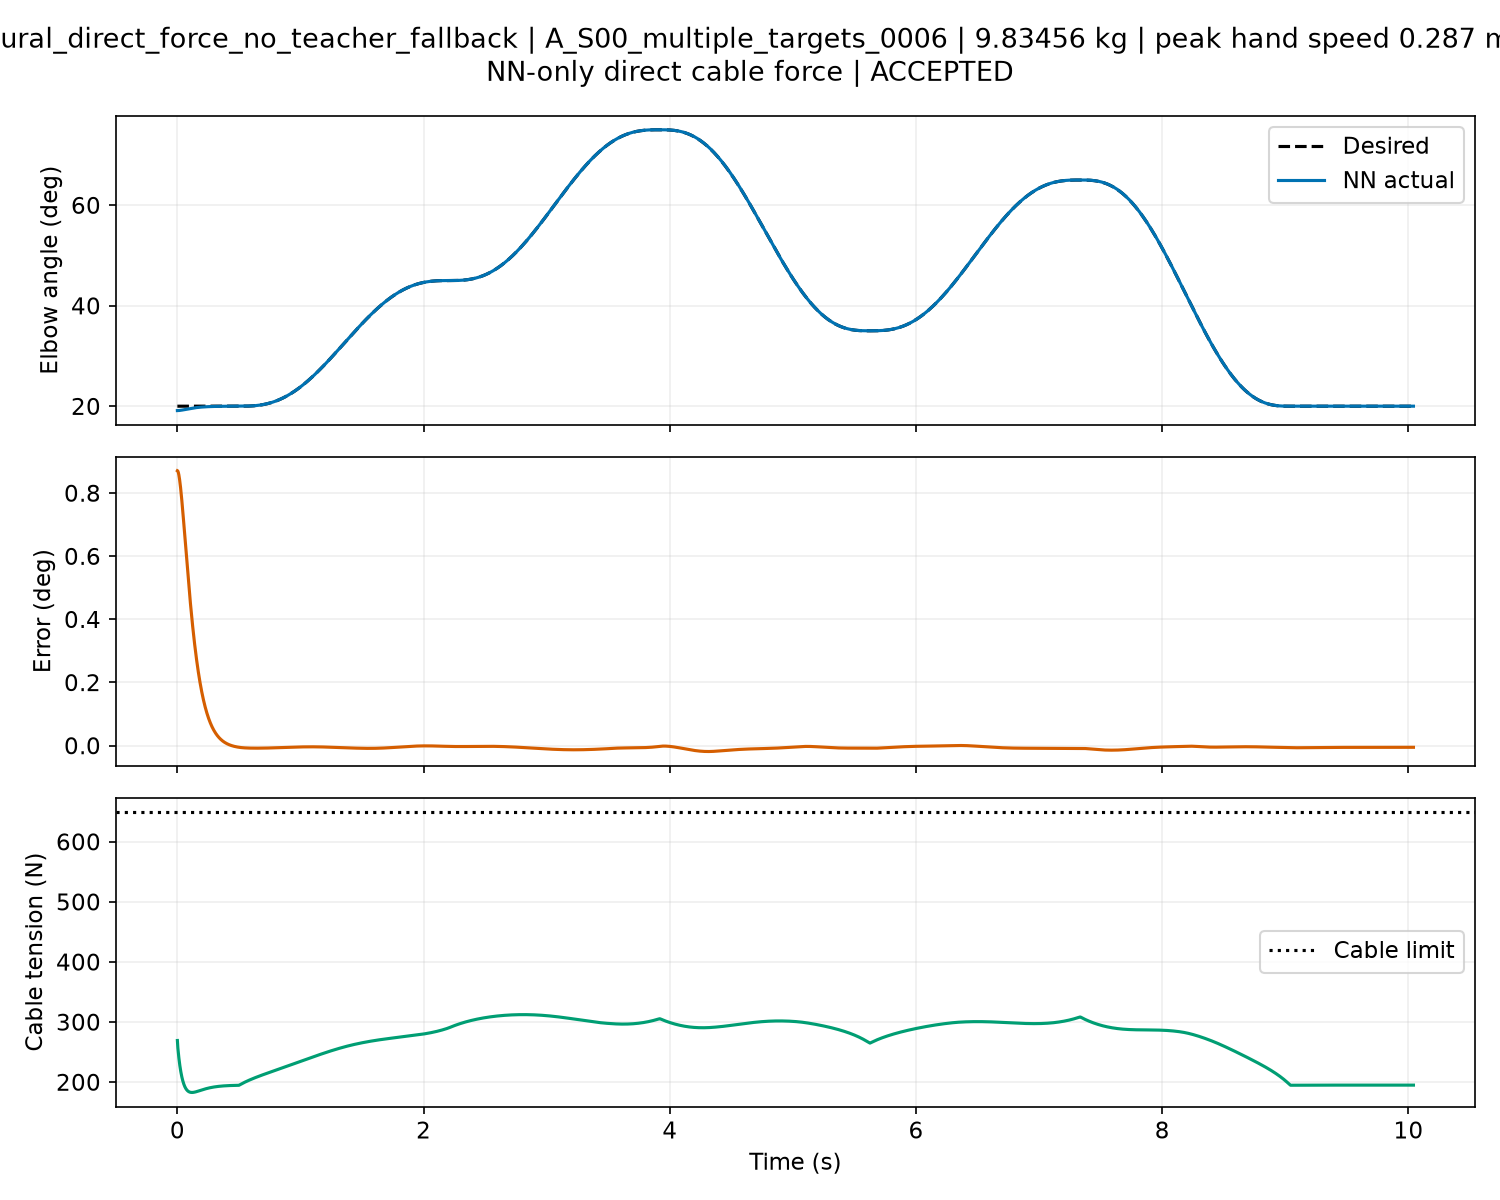
\includegraphics[width=\linewidth,height=0.69\textheight,keepaspectratio]{overleaf_figures/tracking_A_S00_multiple_targets_0006_tracking.png}
\caption{tracking/A\_S00\_multiple\_targets\_0006/tracking.png: Saved simulation diagnostics. Quantities and units are identified on the axes; failed runs are retained.}
\label{fig:tracking_A_S00_multiple_targets_0006_tracking}
\end{figure}
\begin{figure}[H]\centering
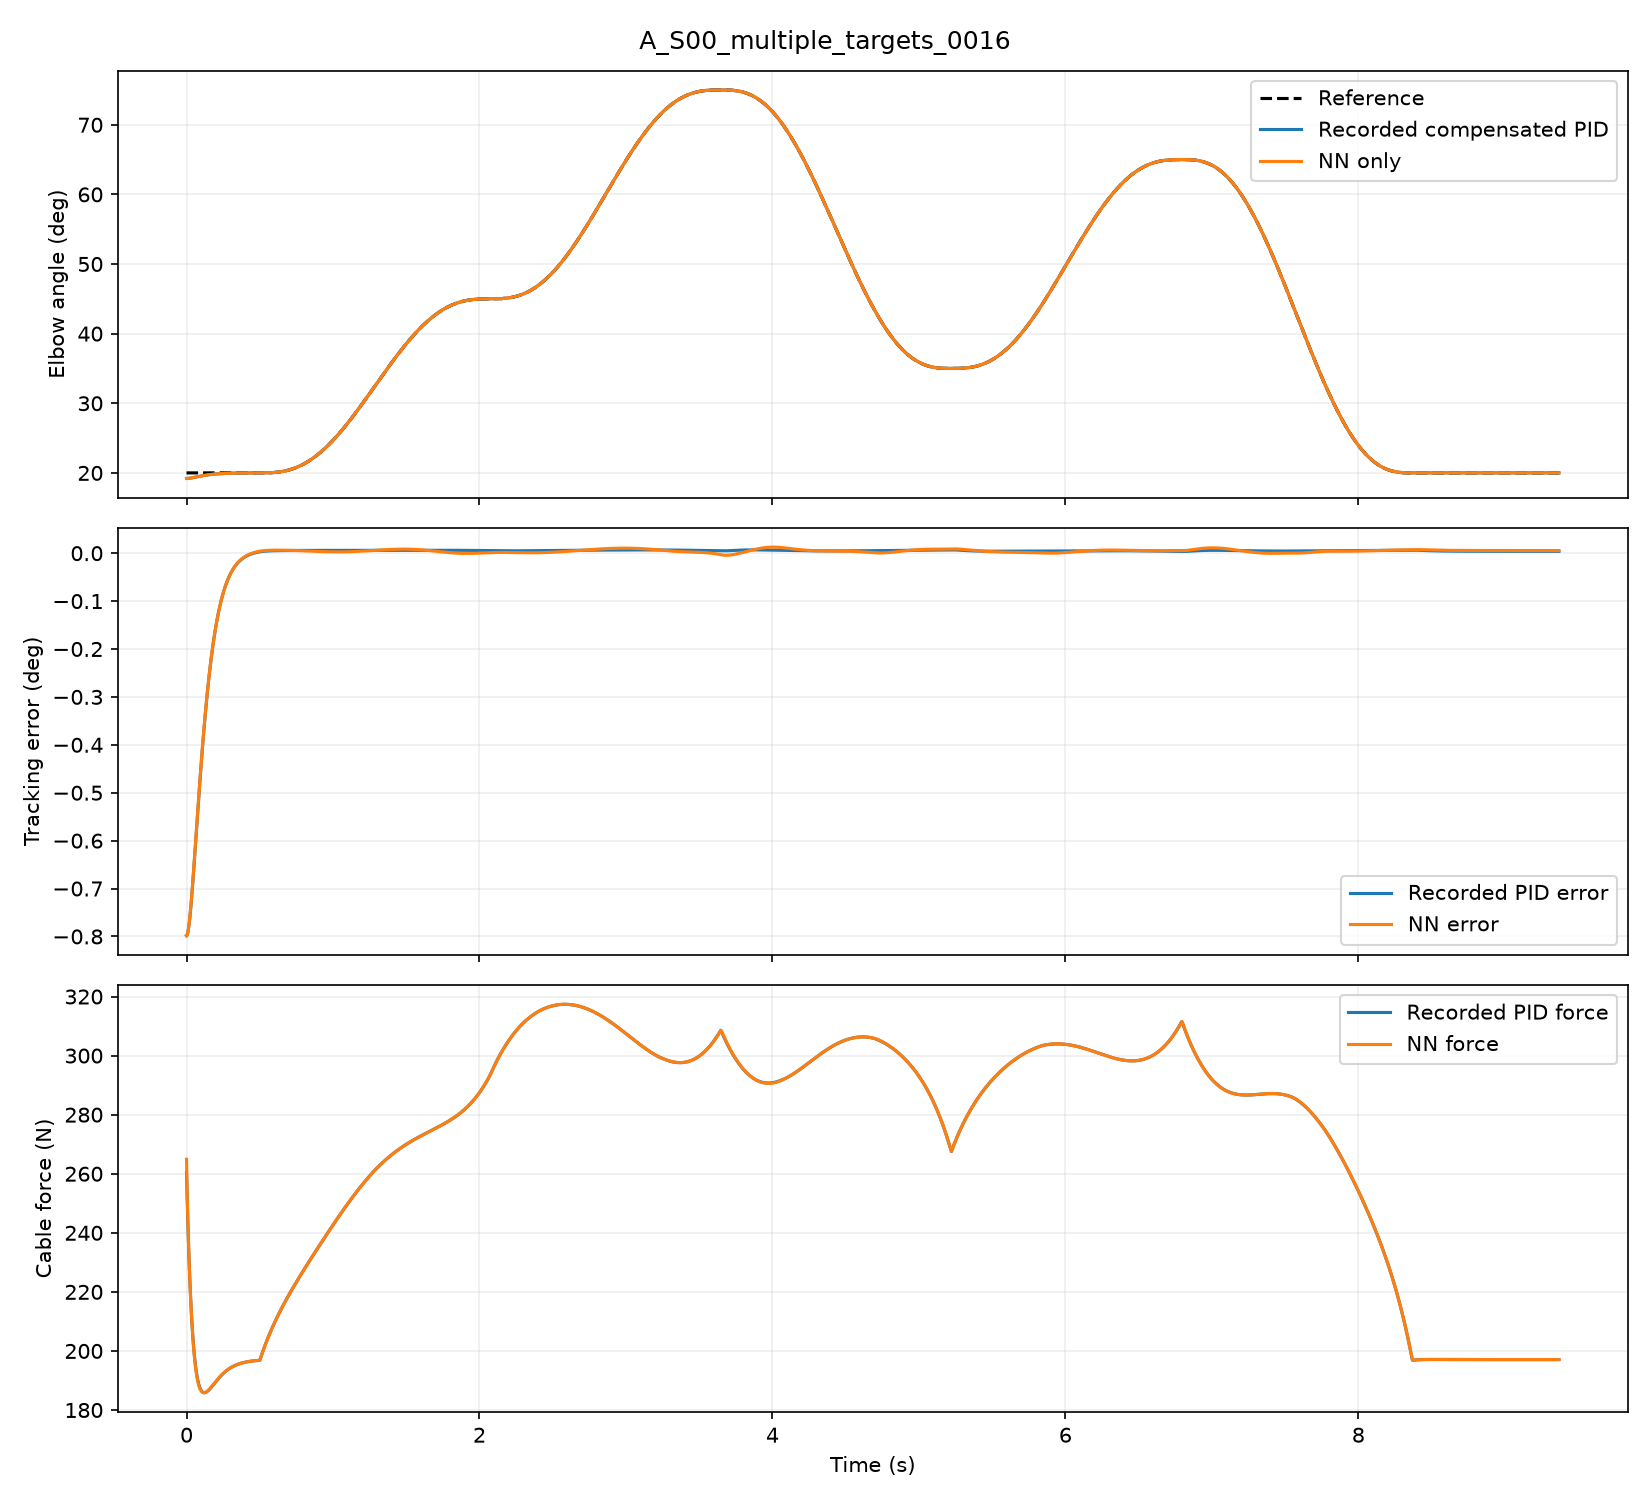
\includegraphics[width=\linewidth,height=0.69\textheight,keepaspectratio]{overleaf_figures/tracking_A_S00_multiple_targets_0016_comparison.png}
\caption{tracking/A\_S00\_multiple\_targets\_0016/comparison.png: Held-out OpenSim rollout: reference, recorded PID, and NN elbow motion; tracking errors; and cable forces. The NN supplies the cable command without a PID fallback.}
\label{fig:tracking_A_S00_multiple_targets_0016_comparison}
\end{figure}
\begin{figure}[H]\centering
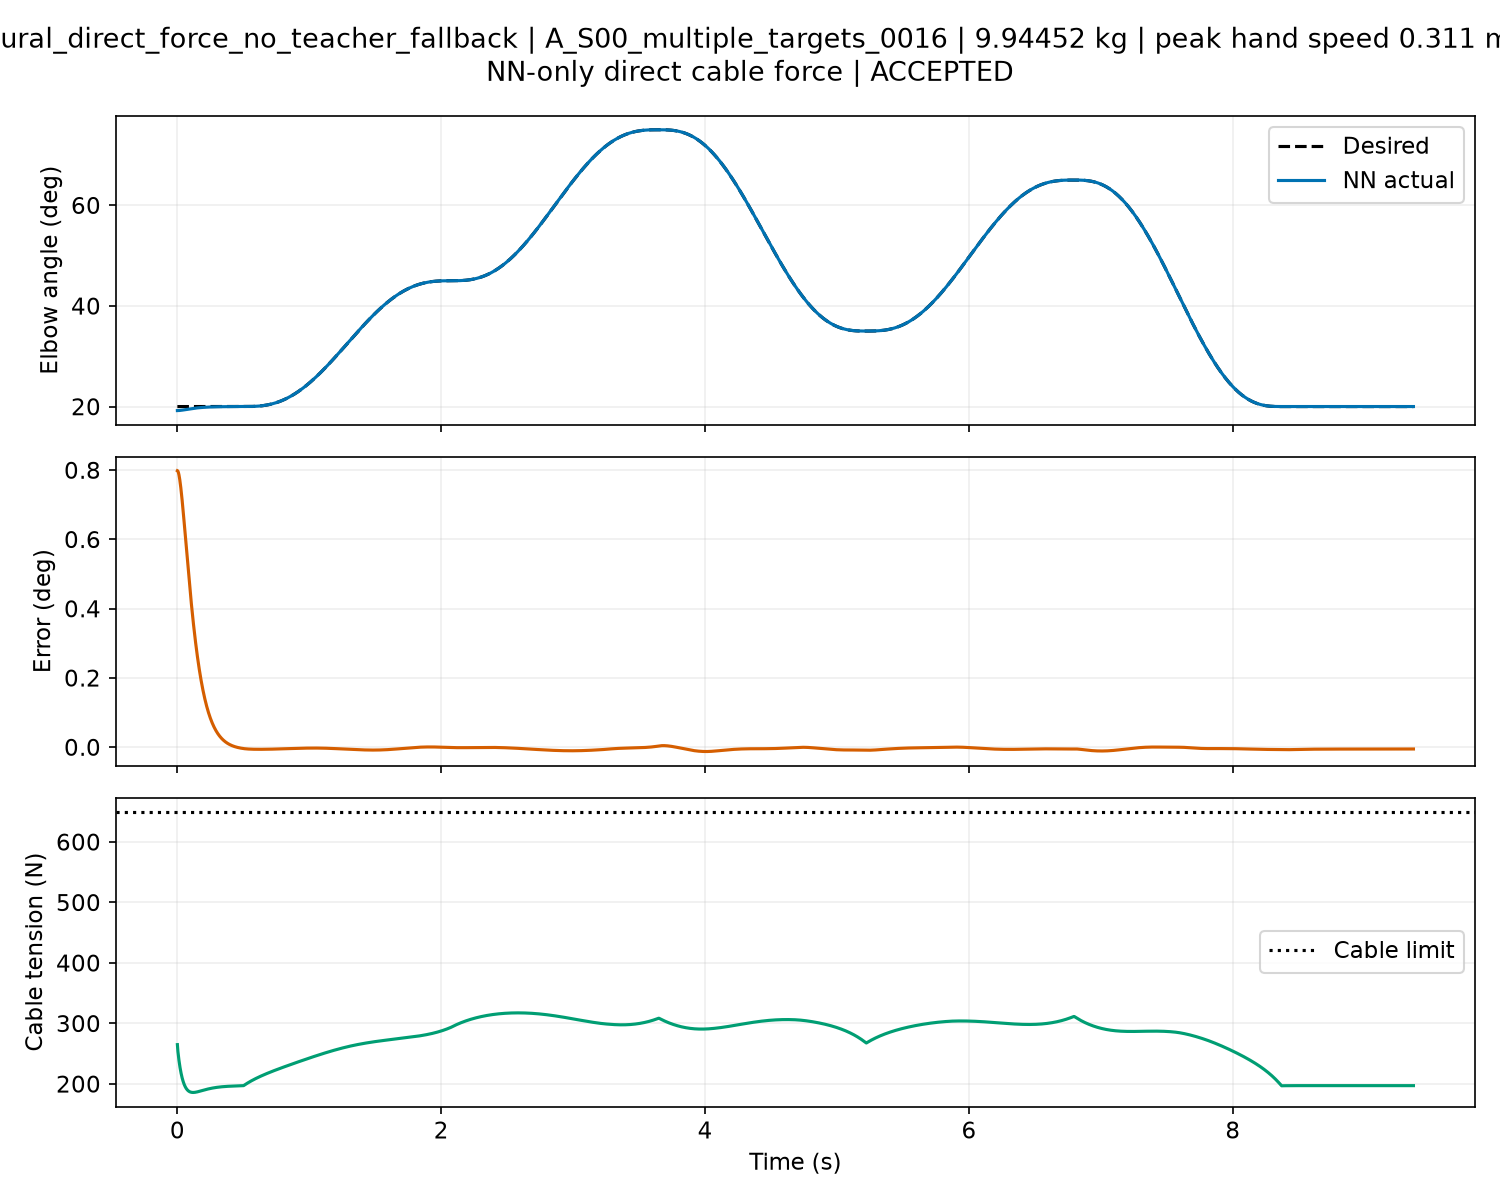
\includegraphics[width=\linewidth,height=0.69\textheight,keepaspectratio]{overleaf_figures/tracking_A_S00_multiple_targets_0016_tracking.png}
\caption{tracking/A\_S00\_multiple\_targets\_0016/tracking.png: Saved simulation diagnostics. Quantities and units are identified on the axes; failed runs are retained.}
\label{fig:tracking_A_S00_multiple_targets_0016_tracking}
\end{figure}
\begin{figure}[H]\centering
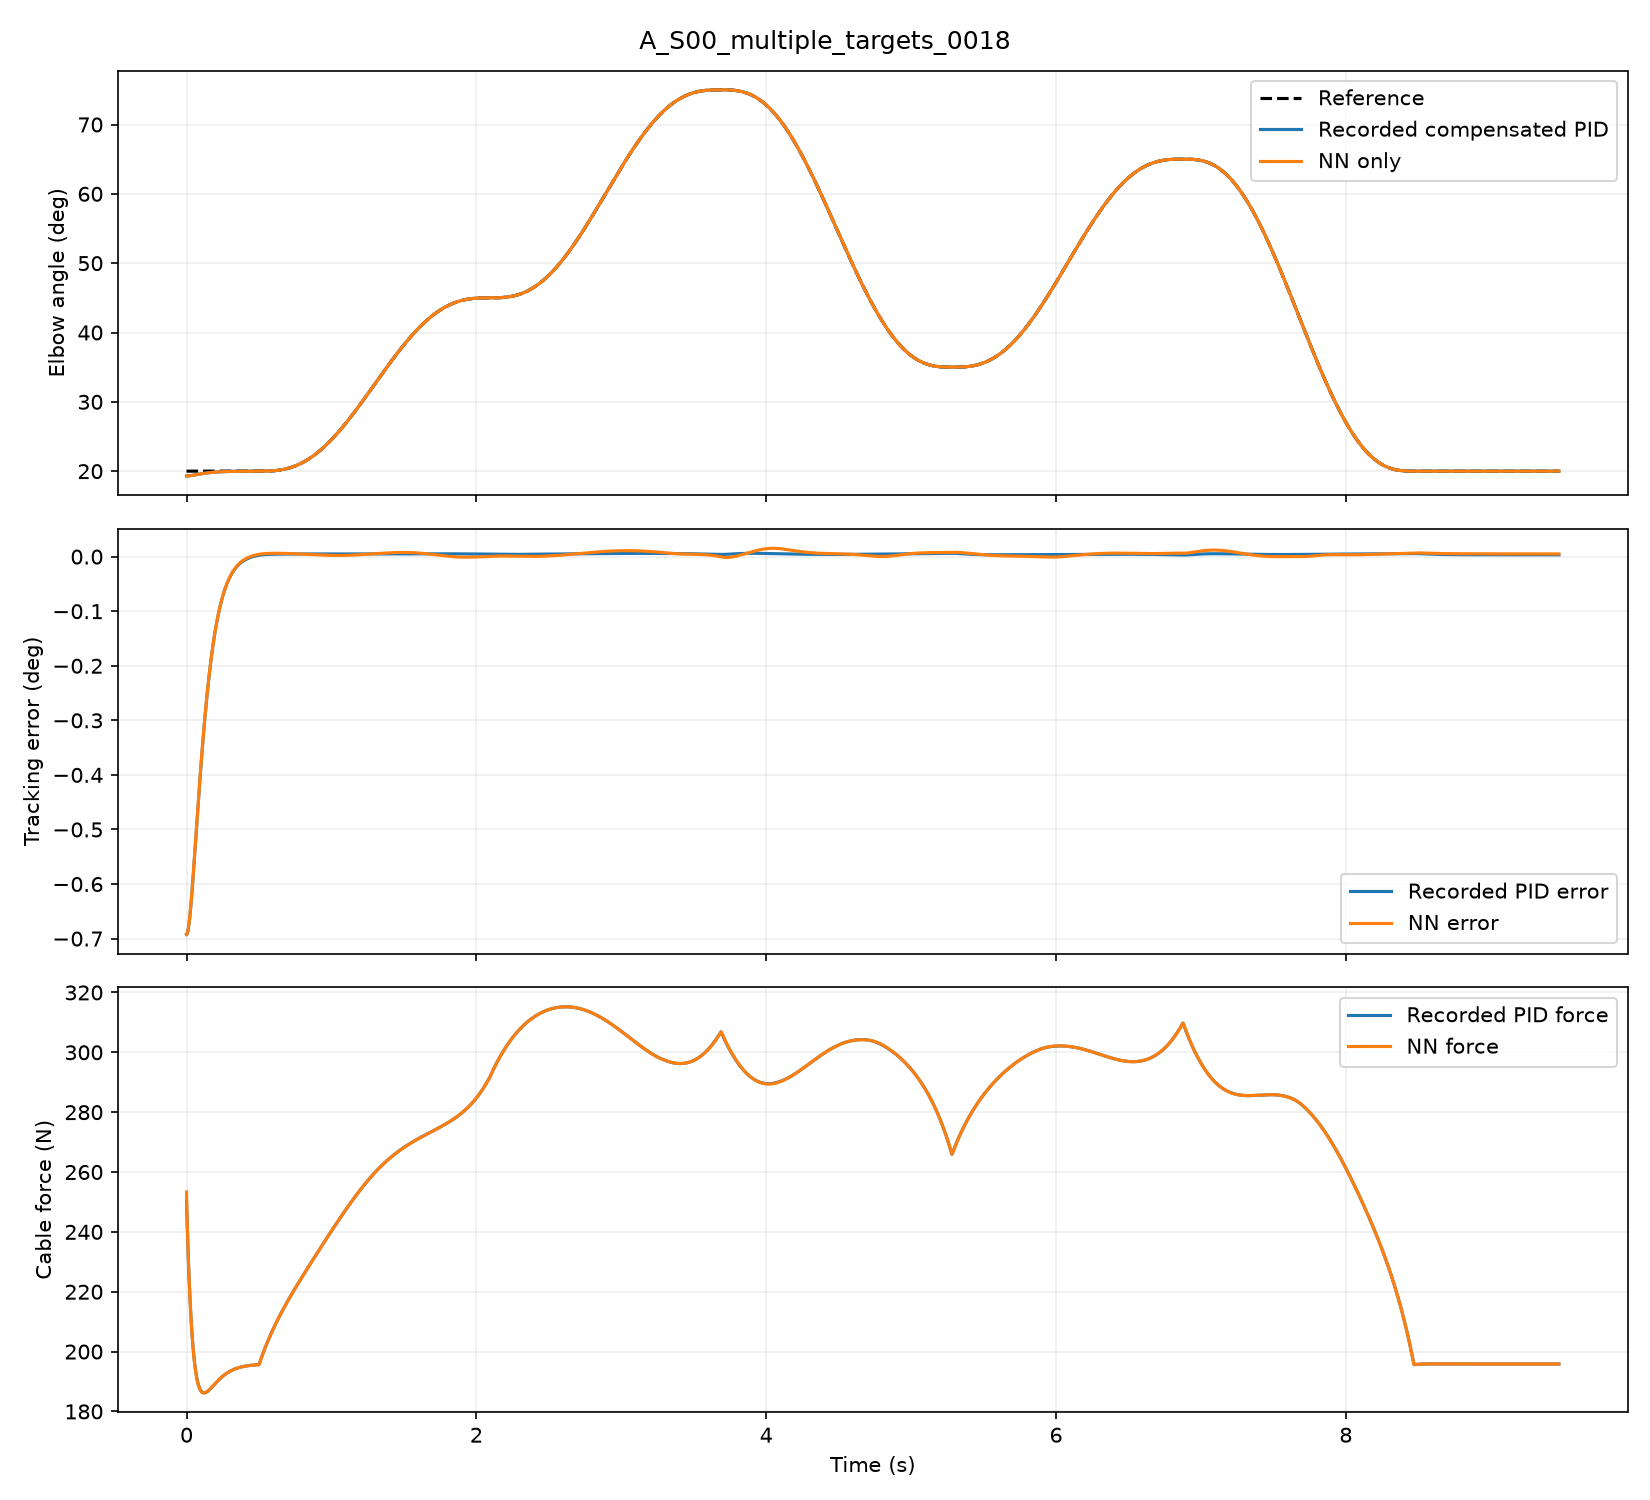
\includegraphics[width=\linewidth,height=0.69\textheight,keepaspectratio]{overleaf_figures/tracking_A_S00_multiple_targets_0018_comparison.png}
\caption{tracking/A\_S00\_multiple\_targets\_0018/comparison.png: Held-out OpenSim rollout: reference, recorded PID, and NN elbow motion; tracking errors; and cable forces. The NN supplies the cable command without a PID fallback.}
\label{fig:tracking_A_S00_multiple_targets_0018_comparison}
\end{figure}
\begin{figure}[H]\centering
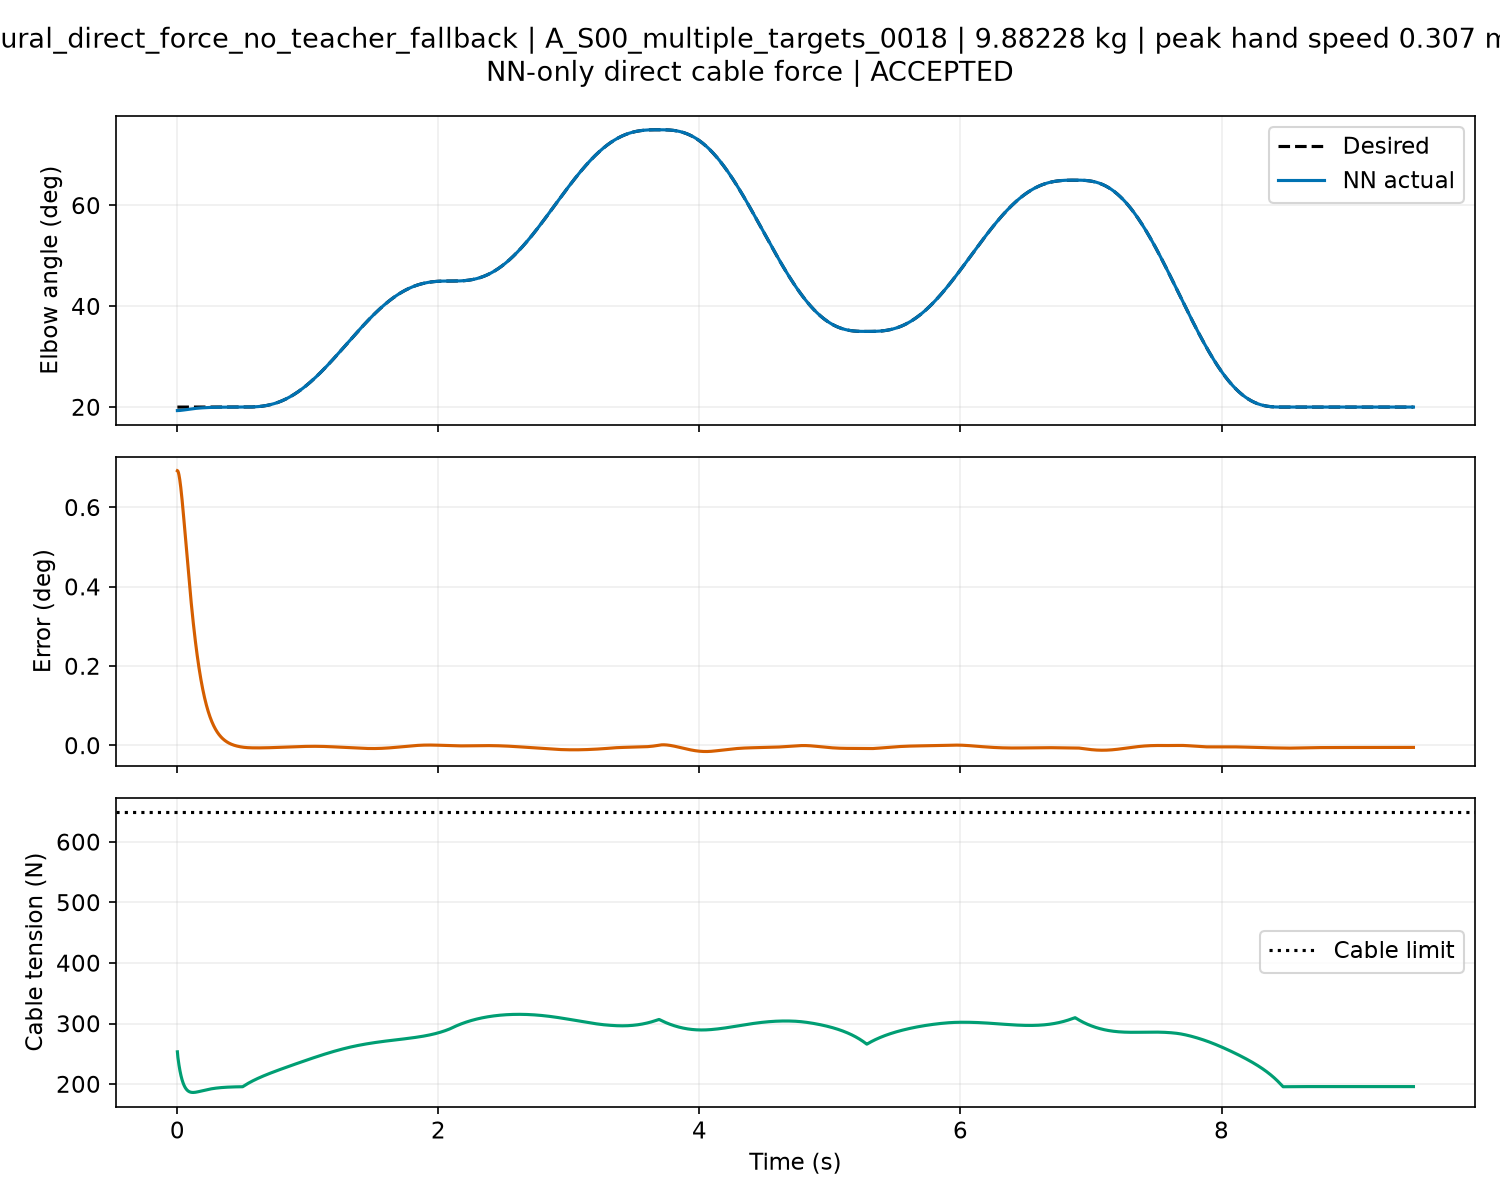
\includegraphics[width=\linewidth,height=0.69\textheight,keepaspectratio]{overleaf_figures/tracking_A_S00_multiple_targets_0018_tracking.png}
\caption{tracking/A\_S00\_multiple\_targets\_0018/tracking.png: Saved simulation diagnostics. Quantities and units are identified on the axes; failed runs are retained.}
\label{fig:tracking_A_S00_multiple_targets_0018_tracking}
\end{figure}
\begin{figure}[H]\centering
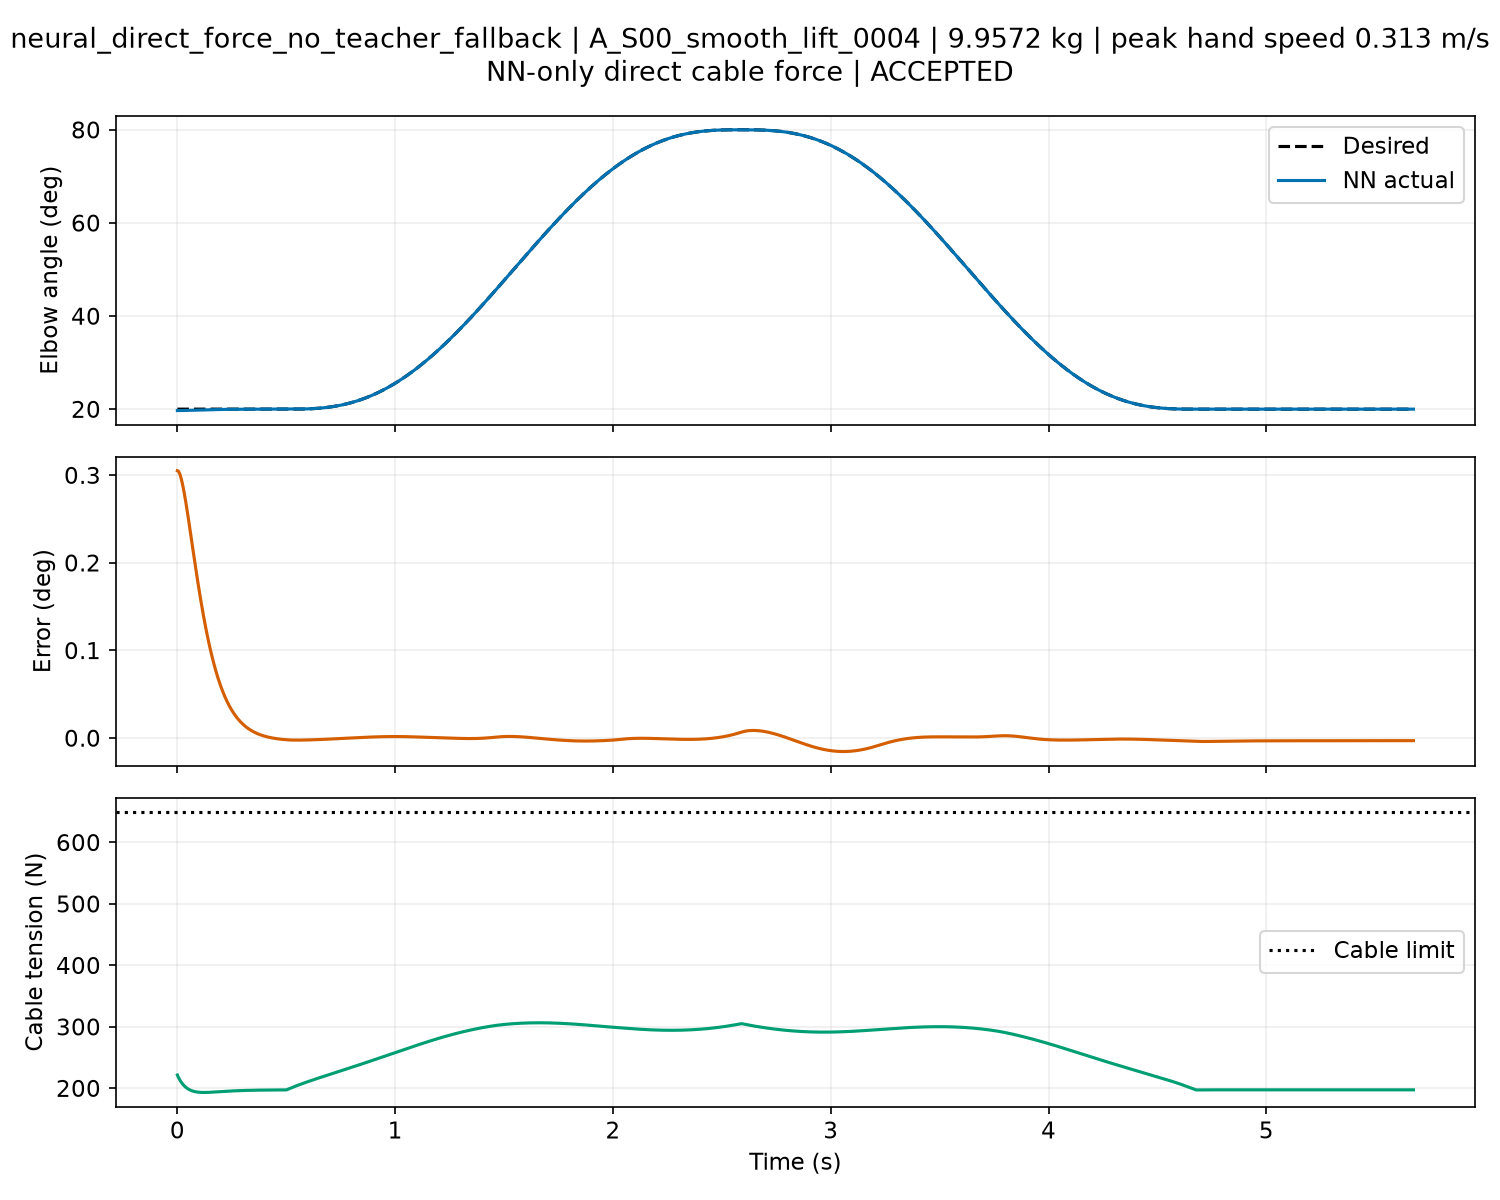
\includegraphics[width=\linewidth,height=0.69\textheight,keepaspectratio]{overleaf_figures/tracking_A_S00_smooth_lift_0004_tracking.png}
\caption{tracking/A\_S00\_smooth\_lift\_0004/tracking.png: Saved simulation diagnostics. Quantities and units are identified on the axes; failed runs are retained.}
\label{fig:tracking_A_S00_smooth_lift_0004_tracking}
\end{figure}
\begin{figure}[H]\centering
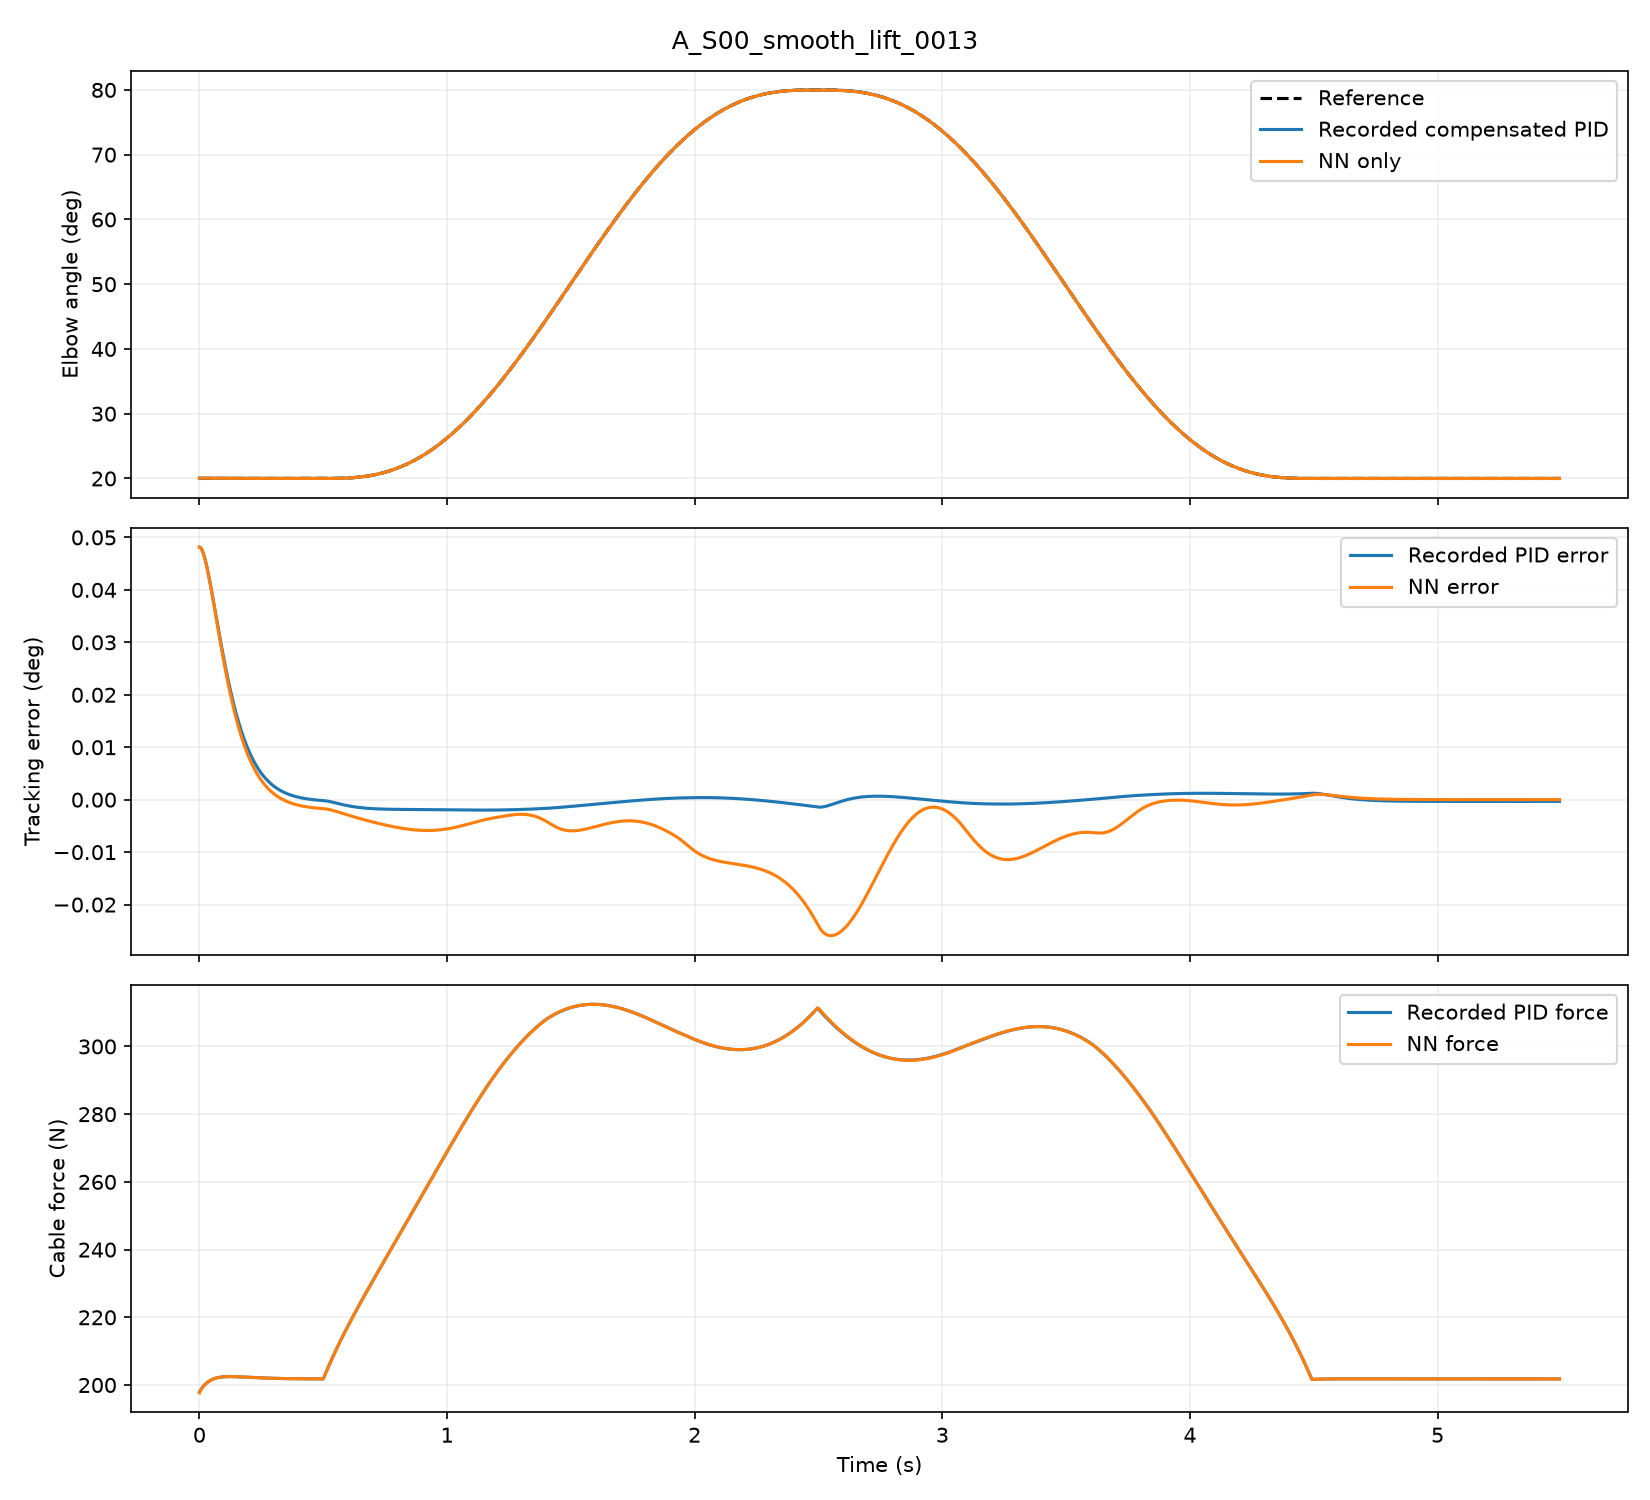
\includegraphics[width=\linewidth,height=0.69\textheight,keepaspectratio]{overleaf_figures/tracking_A_S00_smooth_lift_0013_comparison.png}
\caption{tracking/A\_S00\_smooth\_lift\_0013/comparison.png: Held-out OpenSim rollout: reference, recorded PID, and NN elbow motion; tracking errors; and cable forces. The NN supplies the cable command without a PID fallback.}
\label{fig:tracking_A_S00_smooth_lift_0013_comparison}
\end{figure}
\begin{figure}[H]\centering
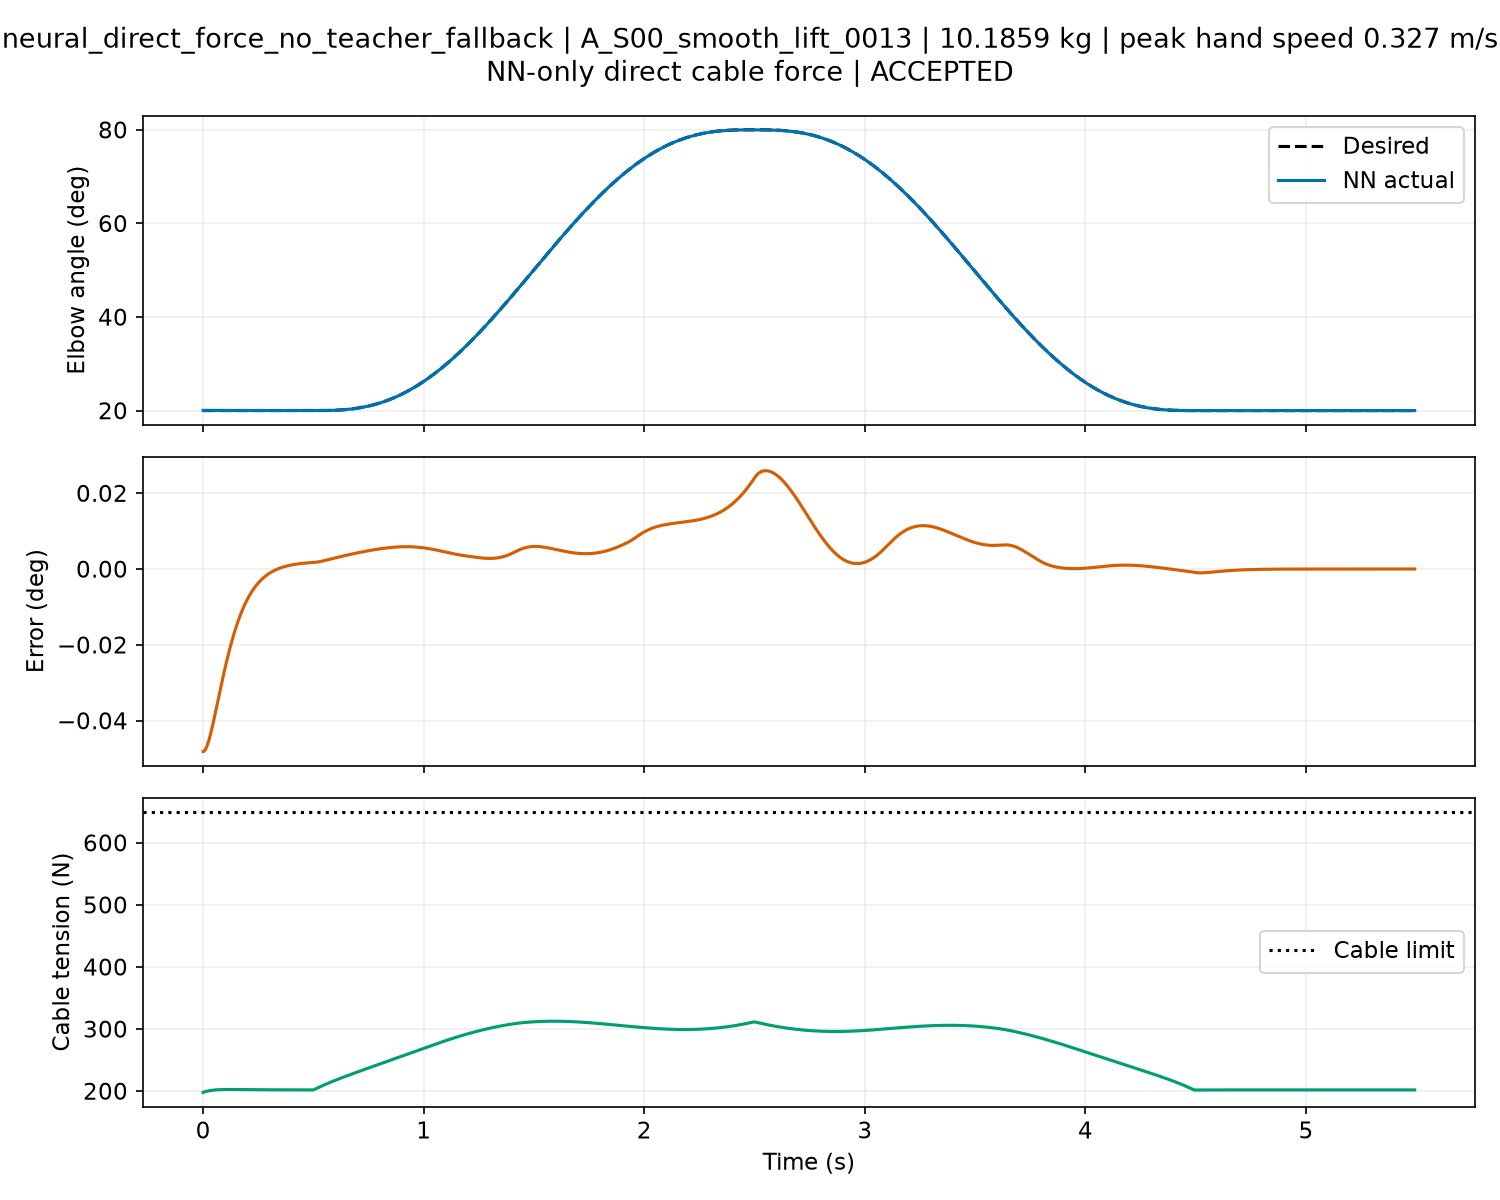
\includegraphics[width=\linewidth,height=0.69\textheight,keepaspectratio]{overleaf_figures/tracking_A_S00_smooth_lift_0013_tracking.png}
\caption{tracking/A\_S00\_smooth\_lift\_0013/tracking.png: Saved simulation diagnostics. Quantities and units are identified on the axes; failed runs are retained.}
\label{fig:tracking_A_S00_smooth_lift_0013_tracking}
\end{figure}
\begin{figure}[H]\centering
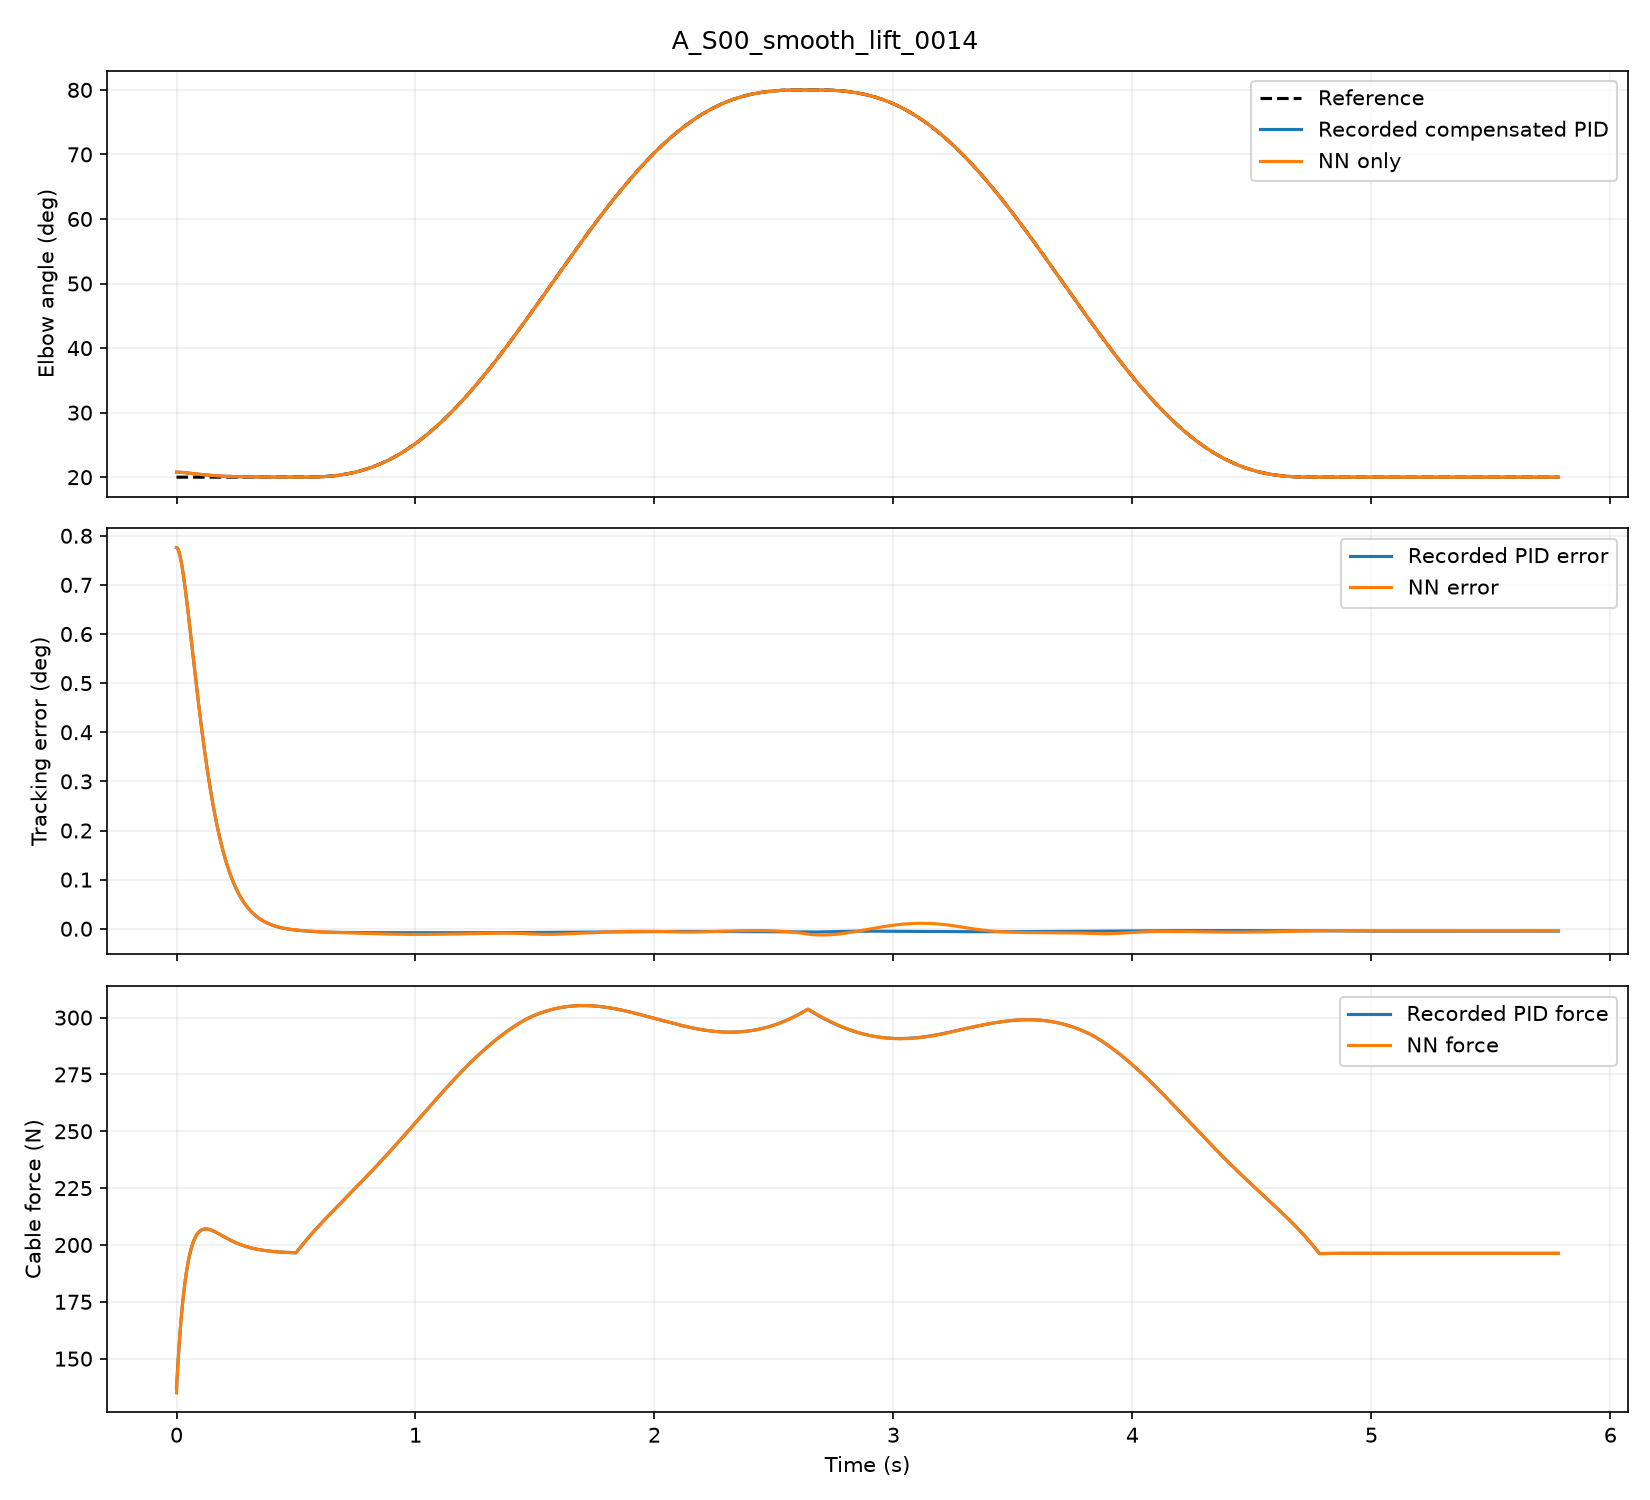
\includegraphics[width=\linewidth,height=0.69\textheight,keepaspectratio]{overleaf_figures/tracking_A_S00_smooth_lift_0014_comparison.png}
\caption{tracking/A\_S00\_smooth\_lift\_0014/comparison.png: Held-out OpenSim rollout: reference, recorded PID, and NN elbow motion; tracking errors; and cable forces. The NN supplies the cable command without a PID fallback.}
\label{fig:tracking_A_S00_smooth_lift_0014_comparison}
\end{figure}
\begin{figure}[H]\centering
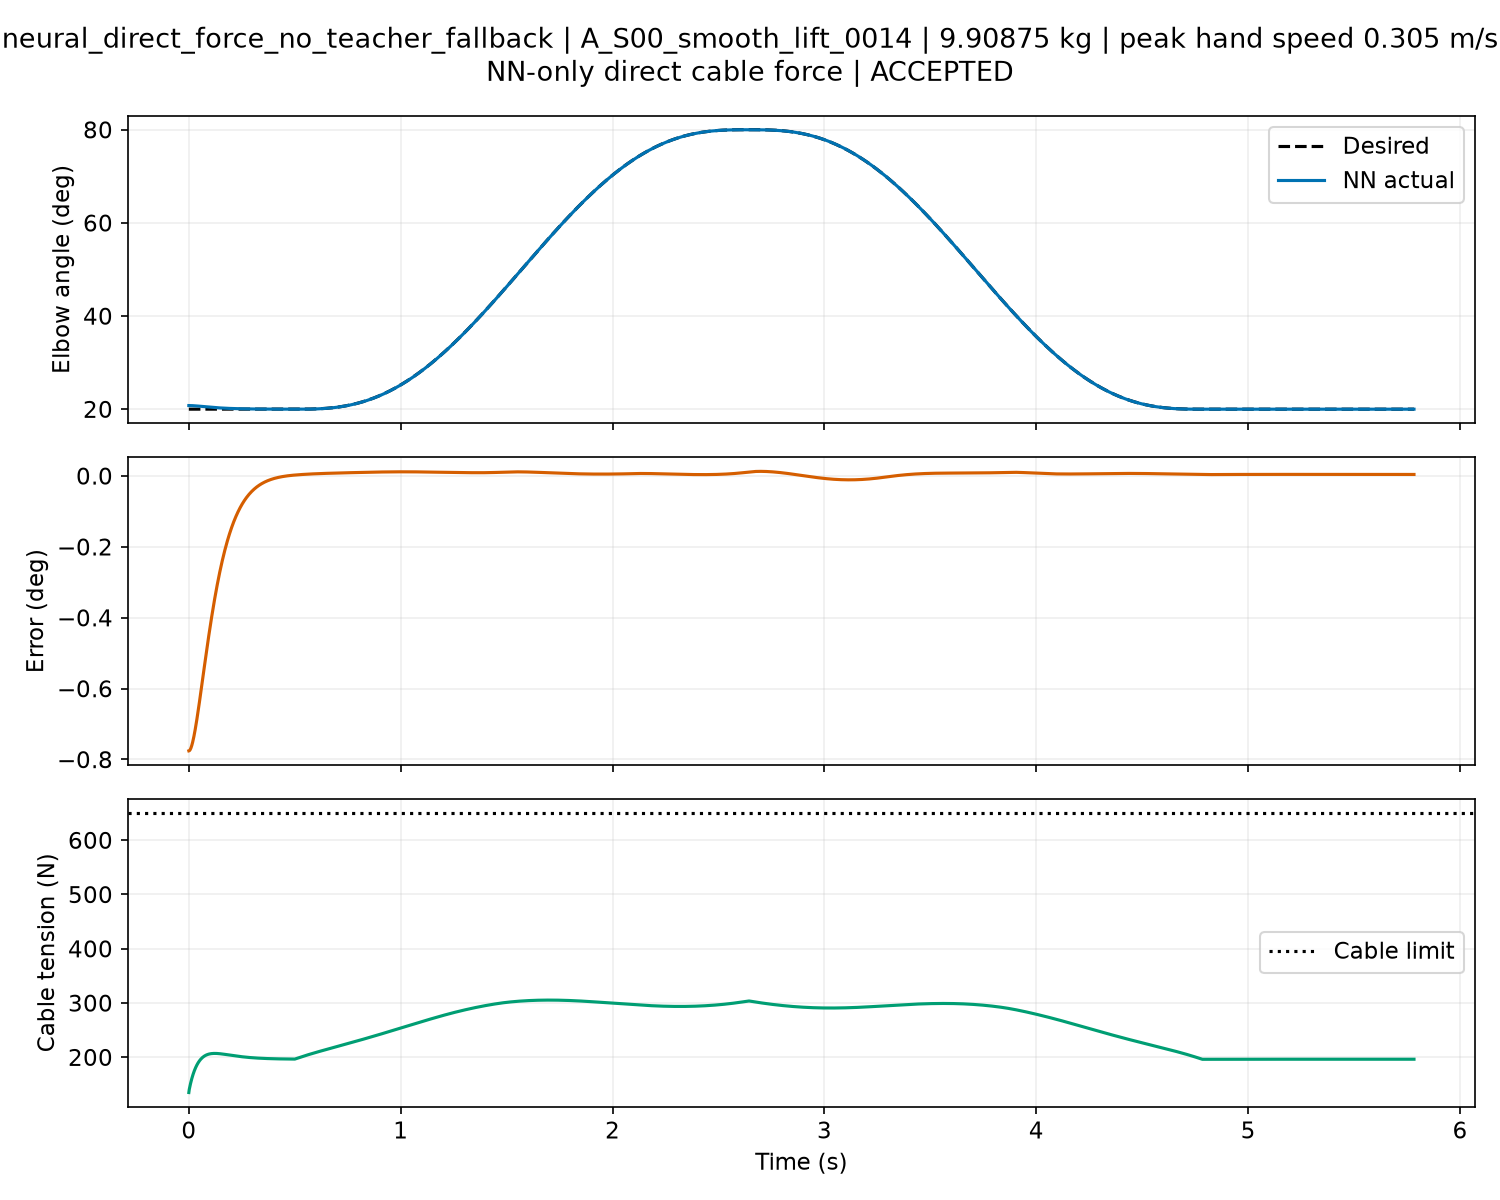
\includegraphics[width=\linewidth,height=0.69\textheight,keepaspectratio]{overleaf_figures/tracking_A_S00_smooth_lift_0014_tracking.png}
\caption{tracking/A\_S00\_smooth\_lift\_0014/tracking.png: Saved simulation diagnostics. Quantities and units are identified on the axes; failed runs are retained.}
\label{fig:tracking_A_S00_smooth_lift_0014_tracking}
\end{figure}
\begin{figure}[H]\centering
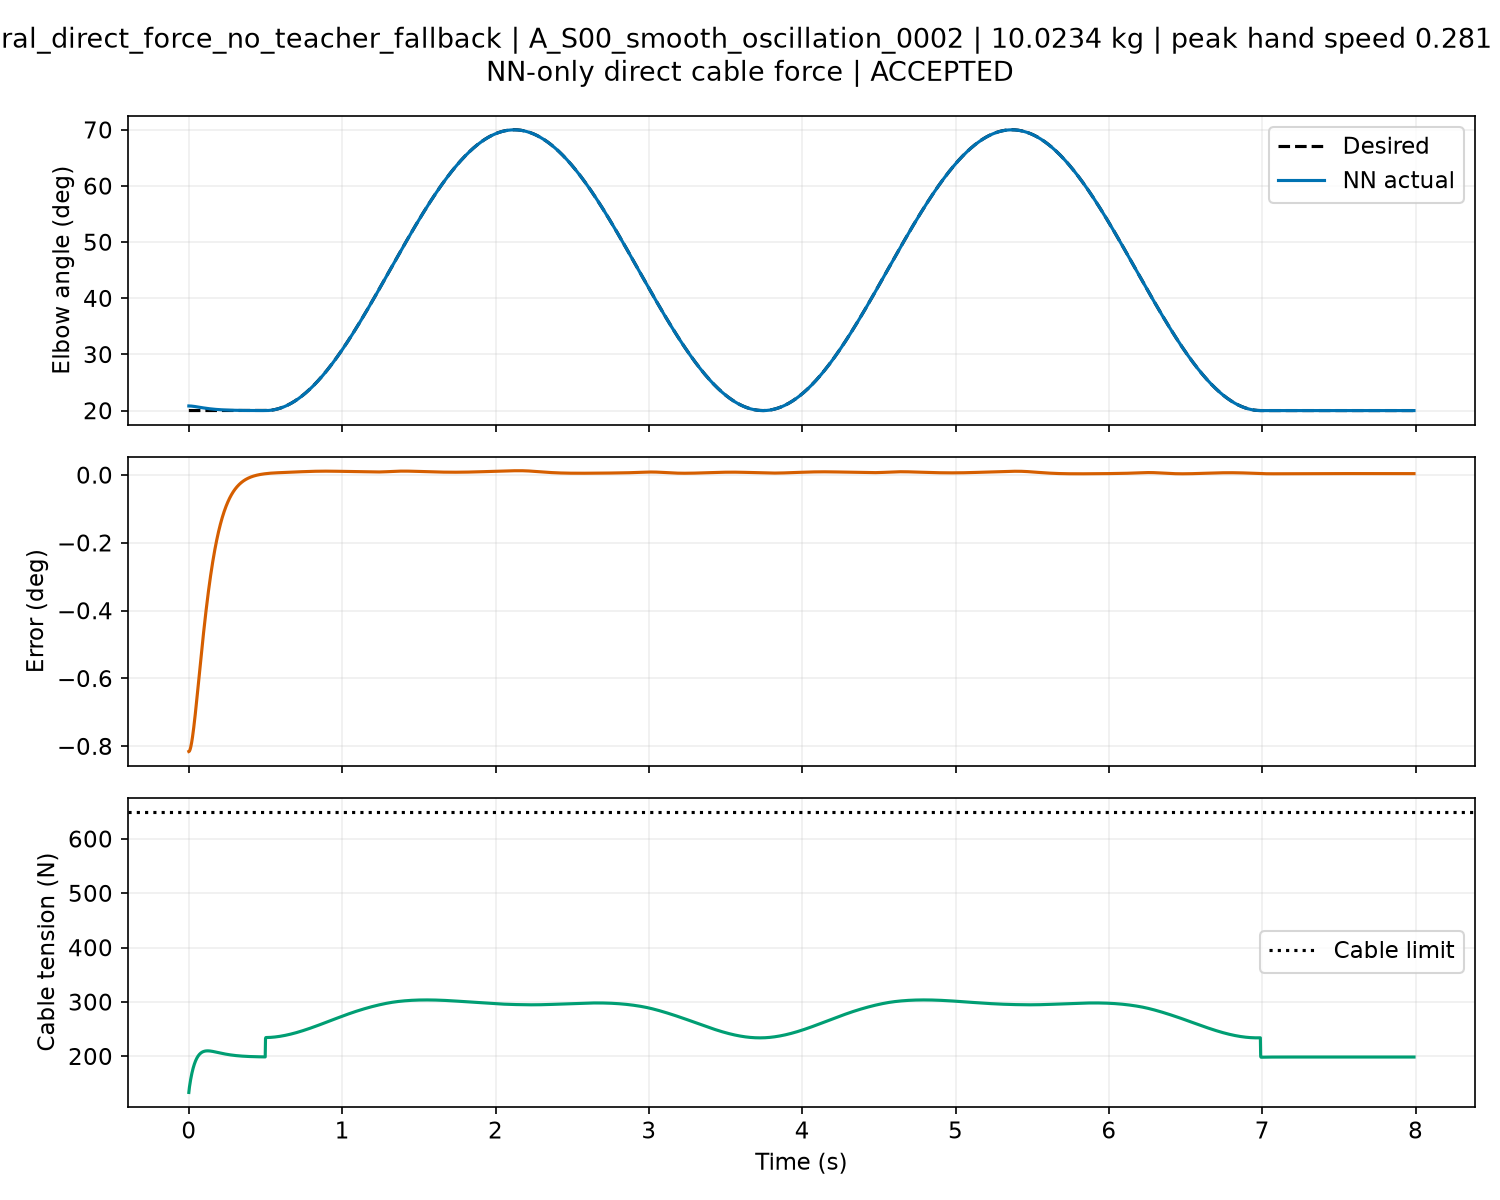
\includegraphics[width=\linewidth,height=0.69\textheight,keepaspectratio]{overleaf_figures/tracking_A_S00_smooth_oscillation_0002_tracking.png}
\caption{tracking/A\_S00\_smooth\_oscillation\_0002/tracking.png: Saved simulation diagnostics. Quantities and units are identified on the axes; failed runs are retained.}
\label{fig:tracking_A_S00_smooth_oscillation_0002_tracking}
\end{figure}
\begin{figure}[H]\centering
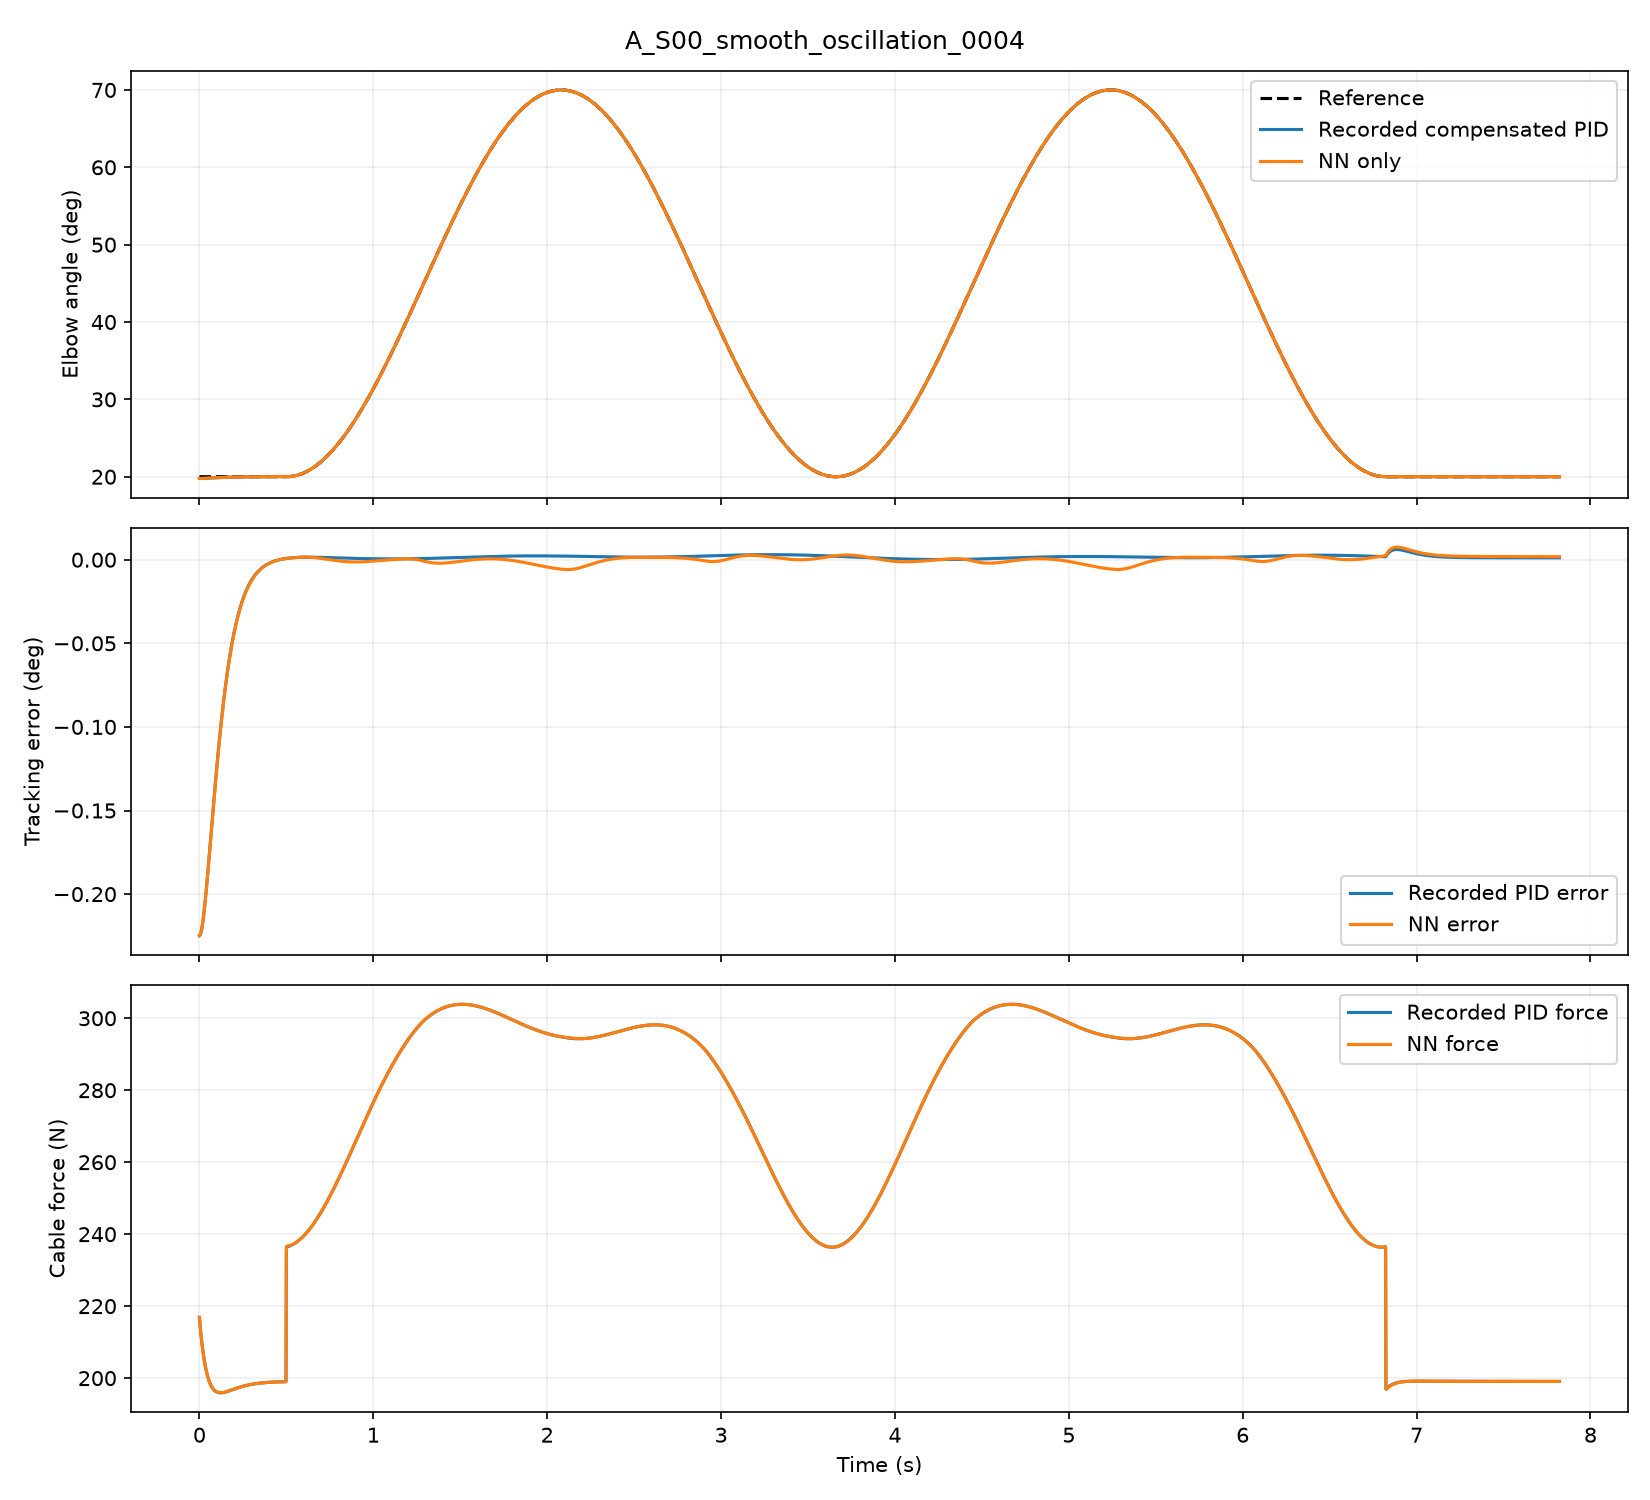
\includegraphics[width=\linewidth,height=0.69\textheight,keepaspectratio]{overleaf_figures/tracking_A_S00_smooth_oscillation_0004_comparison.png}
\caption{tracking/A\_S00\_smooth\_oscillation\_0004/comparison.png: Held-out OpenSim rollout: reference, recorded PID, and NN elbow motion; tracking errors; and cable forces. The NN supplies the cable command without a PID fallback.}
\label{fig:tracking_A_S00_smooth_oscillation_0004_comparison}
\end{figure}
\begin{figure}[H]\centering
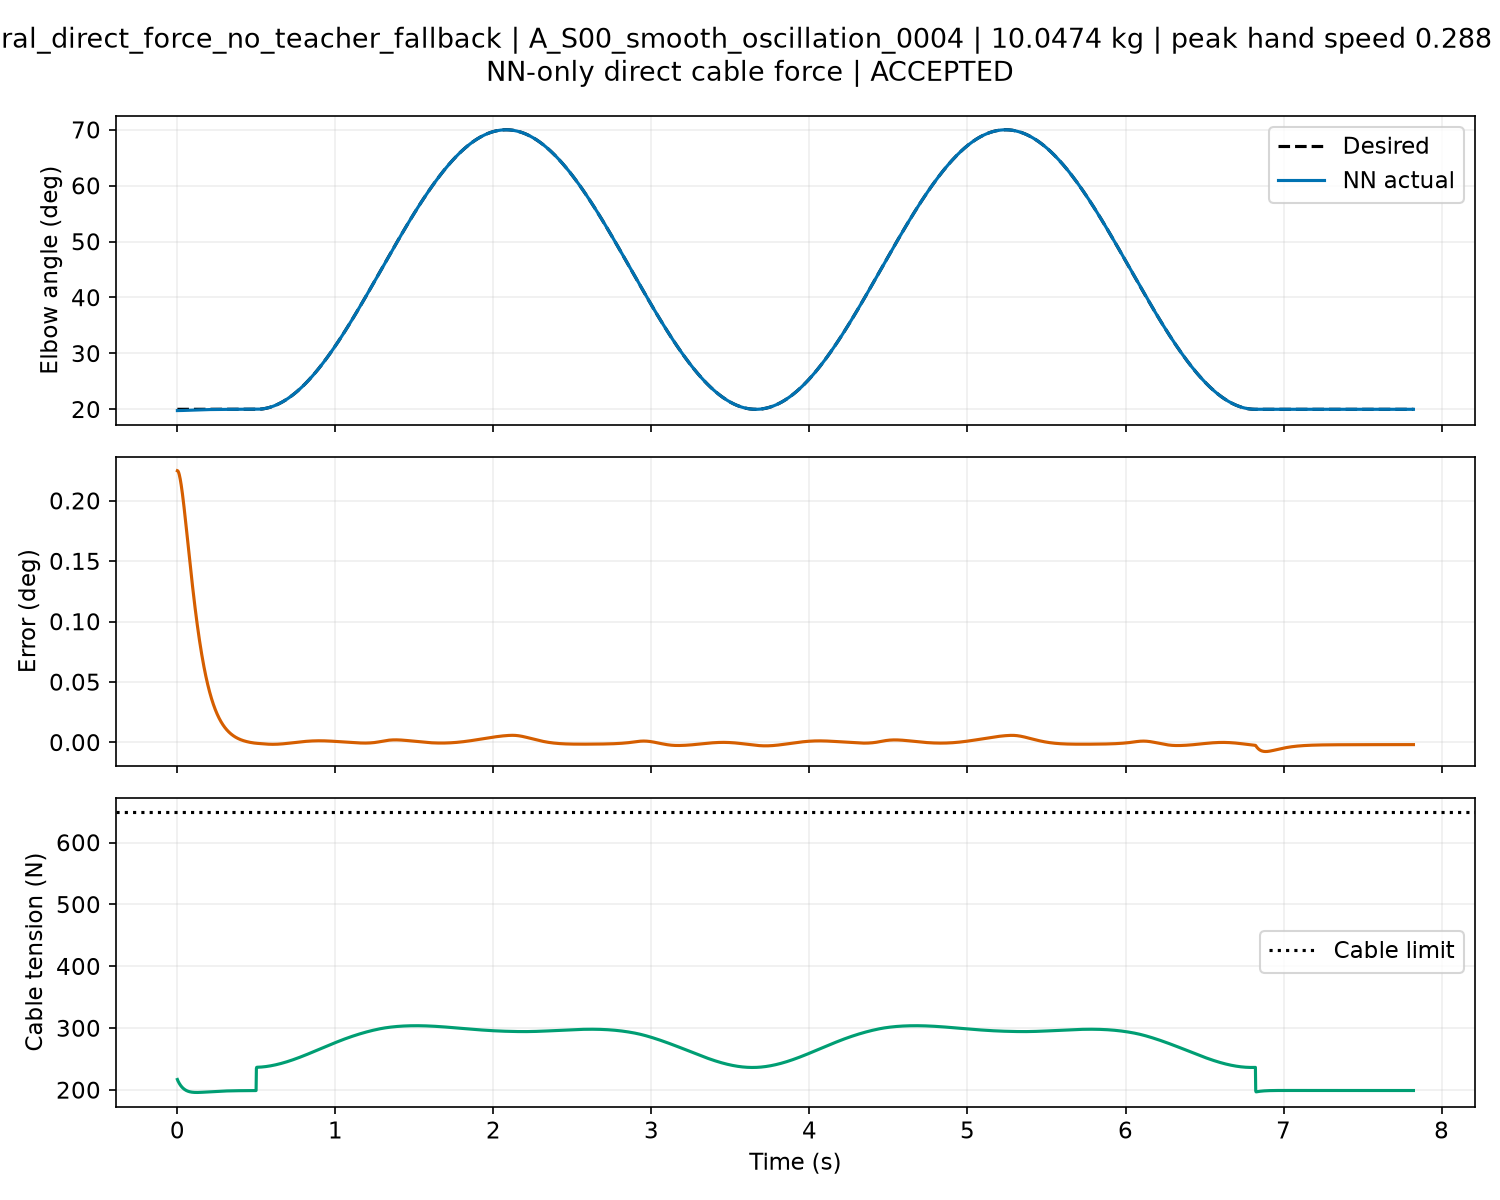
\includegraphics[width=\linewidth,height=0.69\textheight,keepaspectratio]{overleaf_figures/tracking_A_S00_smooth_oscillation_0004_tracking.png}
\caption{tracking/A\_S00\_smooth\_oscillation\_0004/tracking.png: Saved simulation diagnostics. Quantities and units are identified on the axes; failed runs are retained.}
\label{fig:tracking_A_S00_smooth_oscillation_0004_tracking}
\end{figure}
\begin{figure}[H]\centering
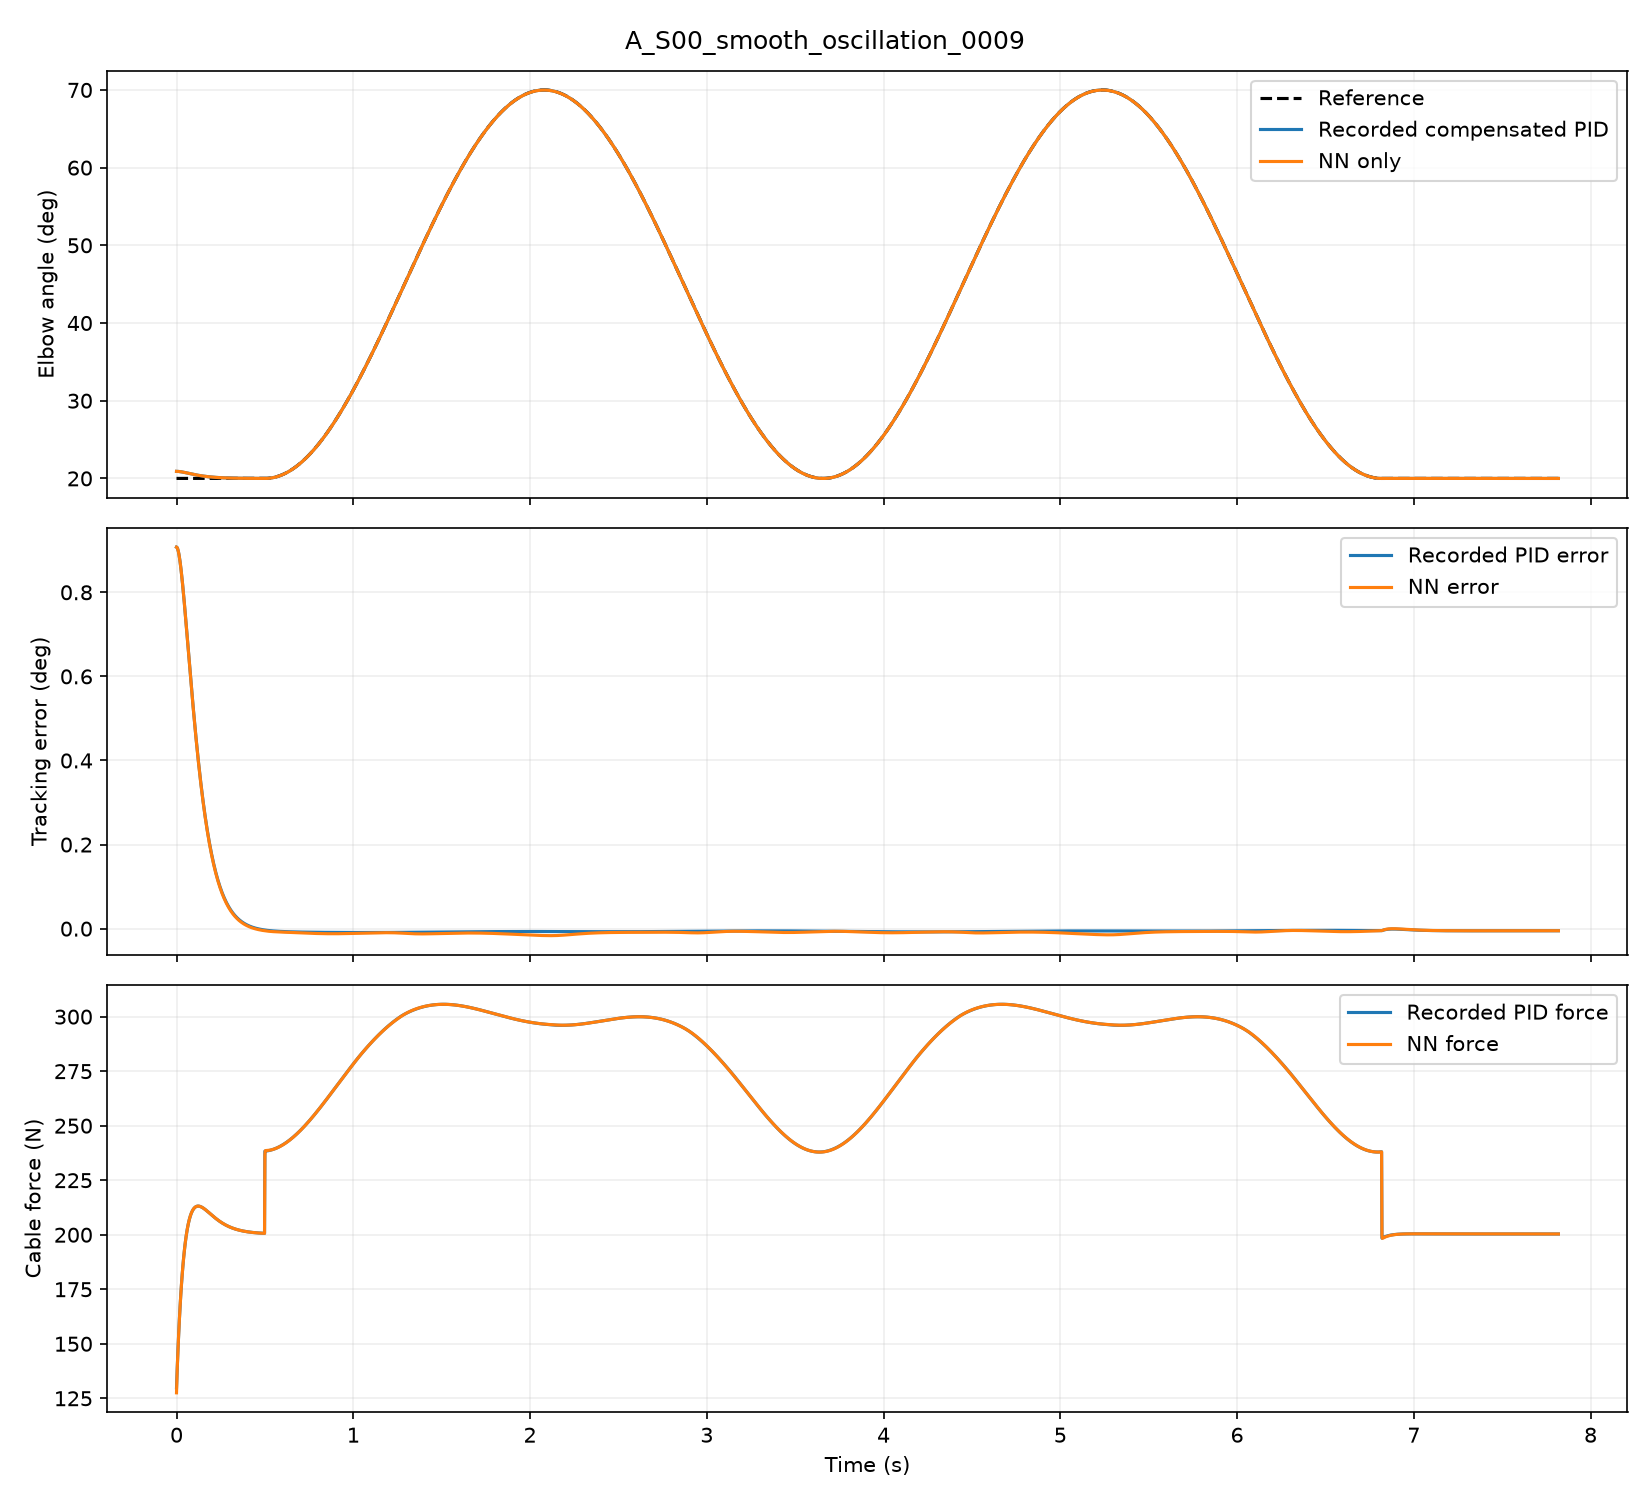
\includegraphics[width=\linewidth,height=0.69\textheight,keepaspectratio]{overleaf_figures/tracking_A_S00_smooth_oscillation_0009_comparison.png}
\caption{tracking/A\_S00\_smooth\_oscillation\_0009/comparison.png: Held-out OpenSim rollout: reference, recorded PID, and NN elbow motion; tracking errors; and cable forces. The NN supplies the cable command without a PID fallback.}
\label{fig:tracking_A_S00_smooth_oscillation_0009_comparison}
\end{figure}
\begin{figure}[H]\centering
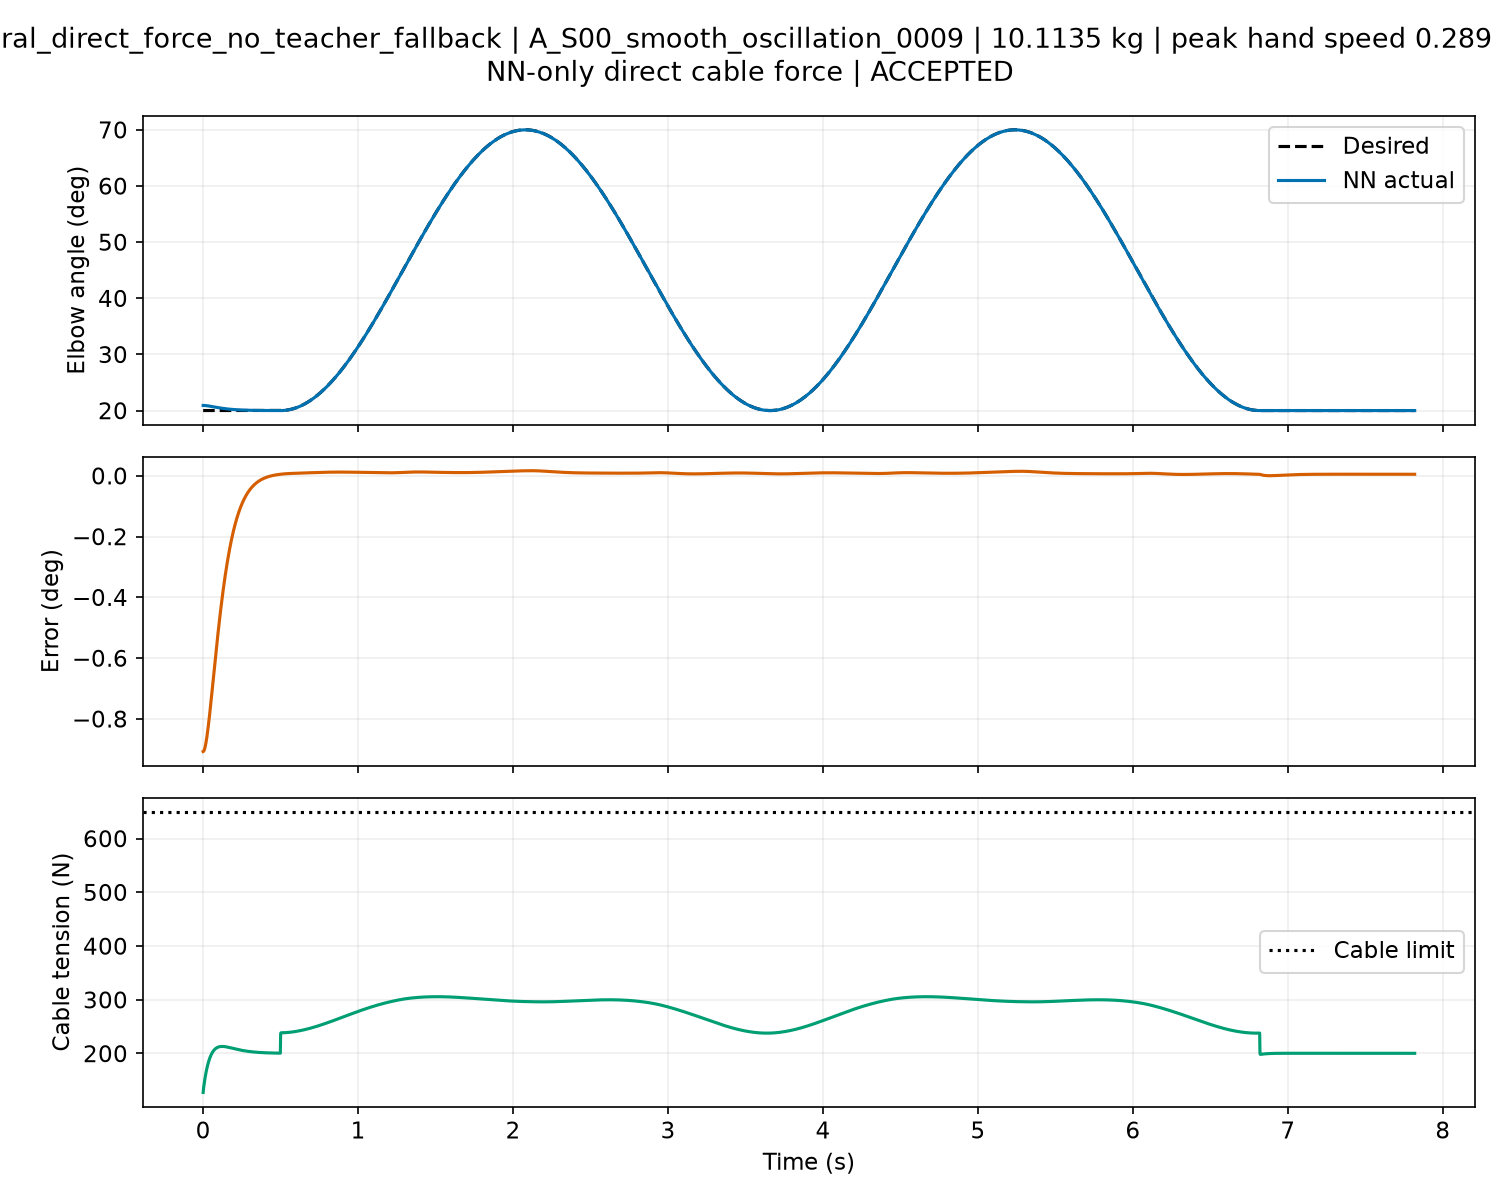
\includegraphics[width=\linewidth,height=0.69\textheight,keepaspectratio]{overleaf_figures/tracking_A_S00_smooth_oscillation_0009_tracking.png}
\caption{tracking/A\_S00\_smooth\_oscillation\_0009/tracking.png: Saved simulation diagnostics. Quantities and units are identified on the axes; failed runs are retained.}
\label{fig:tracking_A_S00_smooth_oscillation_0009_tracking}
\end{figure}
\begin{figure}[H]\centering
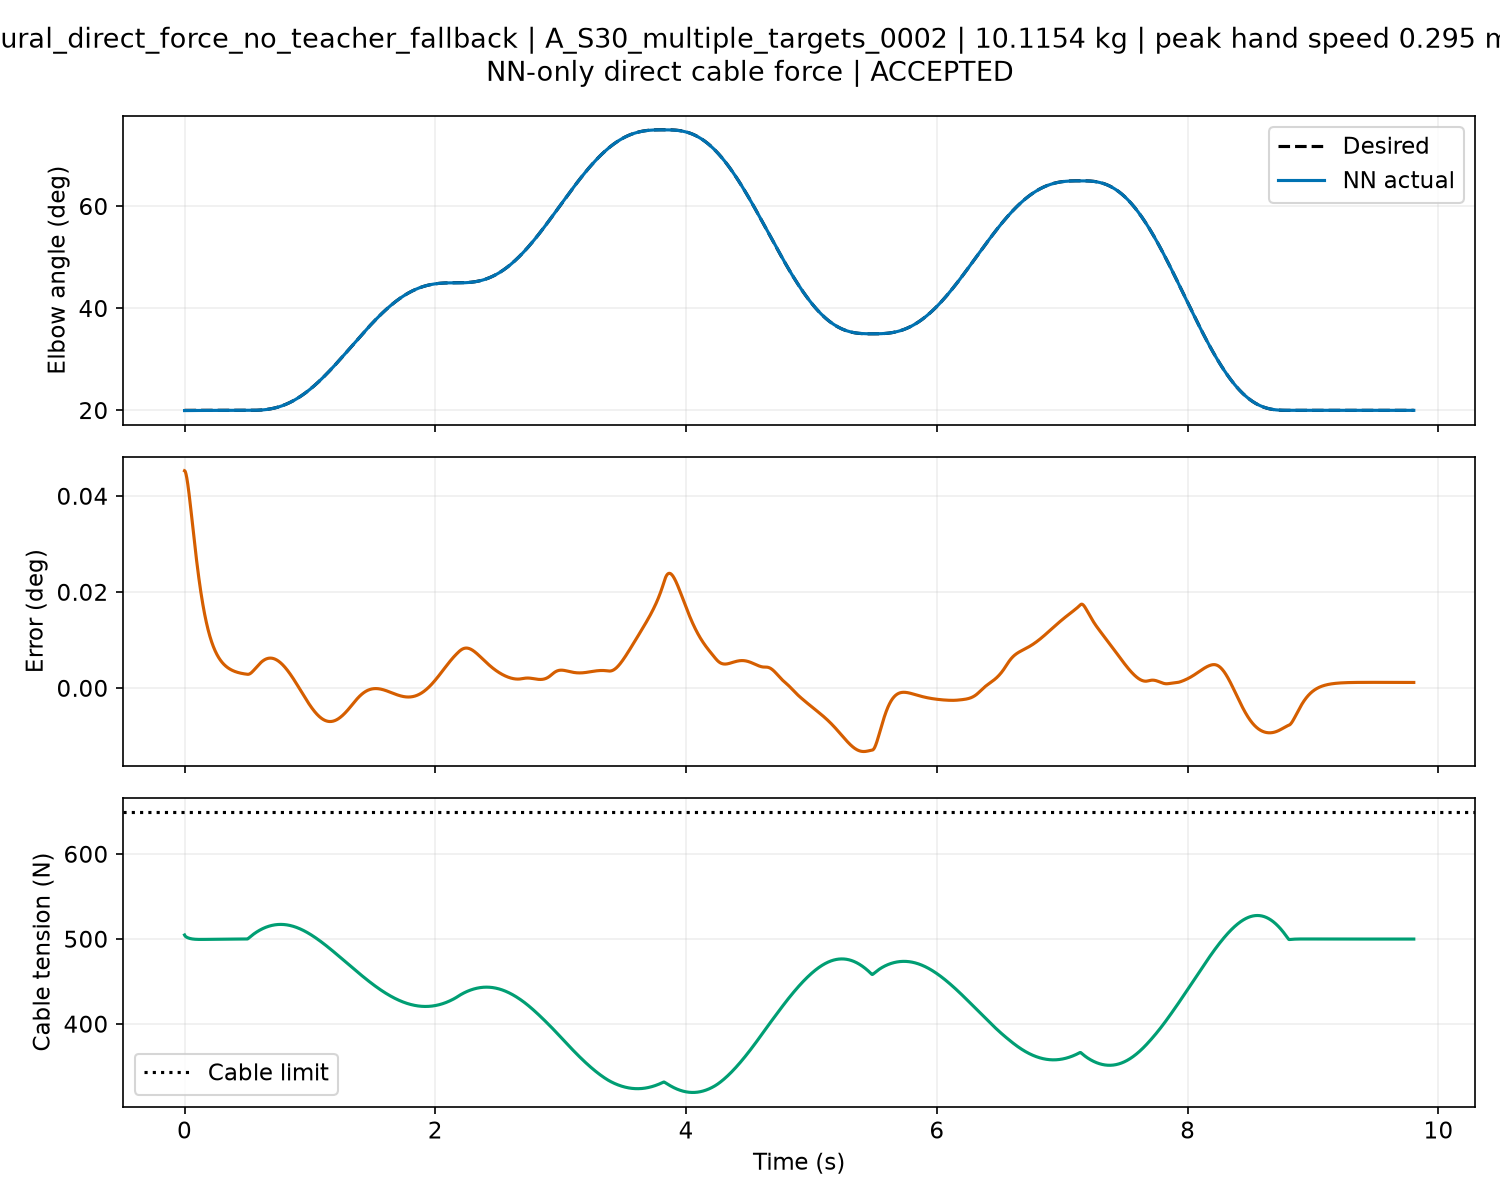
\includegraphics[width=\linewidth,height=0.69\textheight,keepaspectratio]{overleaf_figures/tracking_A_S30_multiple_targets_0002_tracking.png}
\caption{tracking/A\_S30\_multiple\_targets\_0002/tracking.png: Saved simulation diagnostics. Quantities and units are identified on the axes; failed runs are retained.}
\label{fig:tracking_A_S30_multiple_targets_0002_tracking}
\end{figure}
\begin{figure}[H]\centering
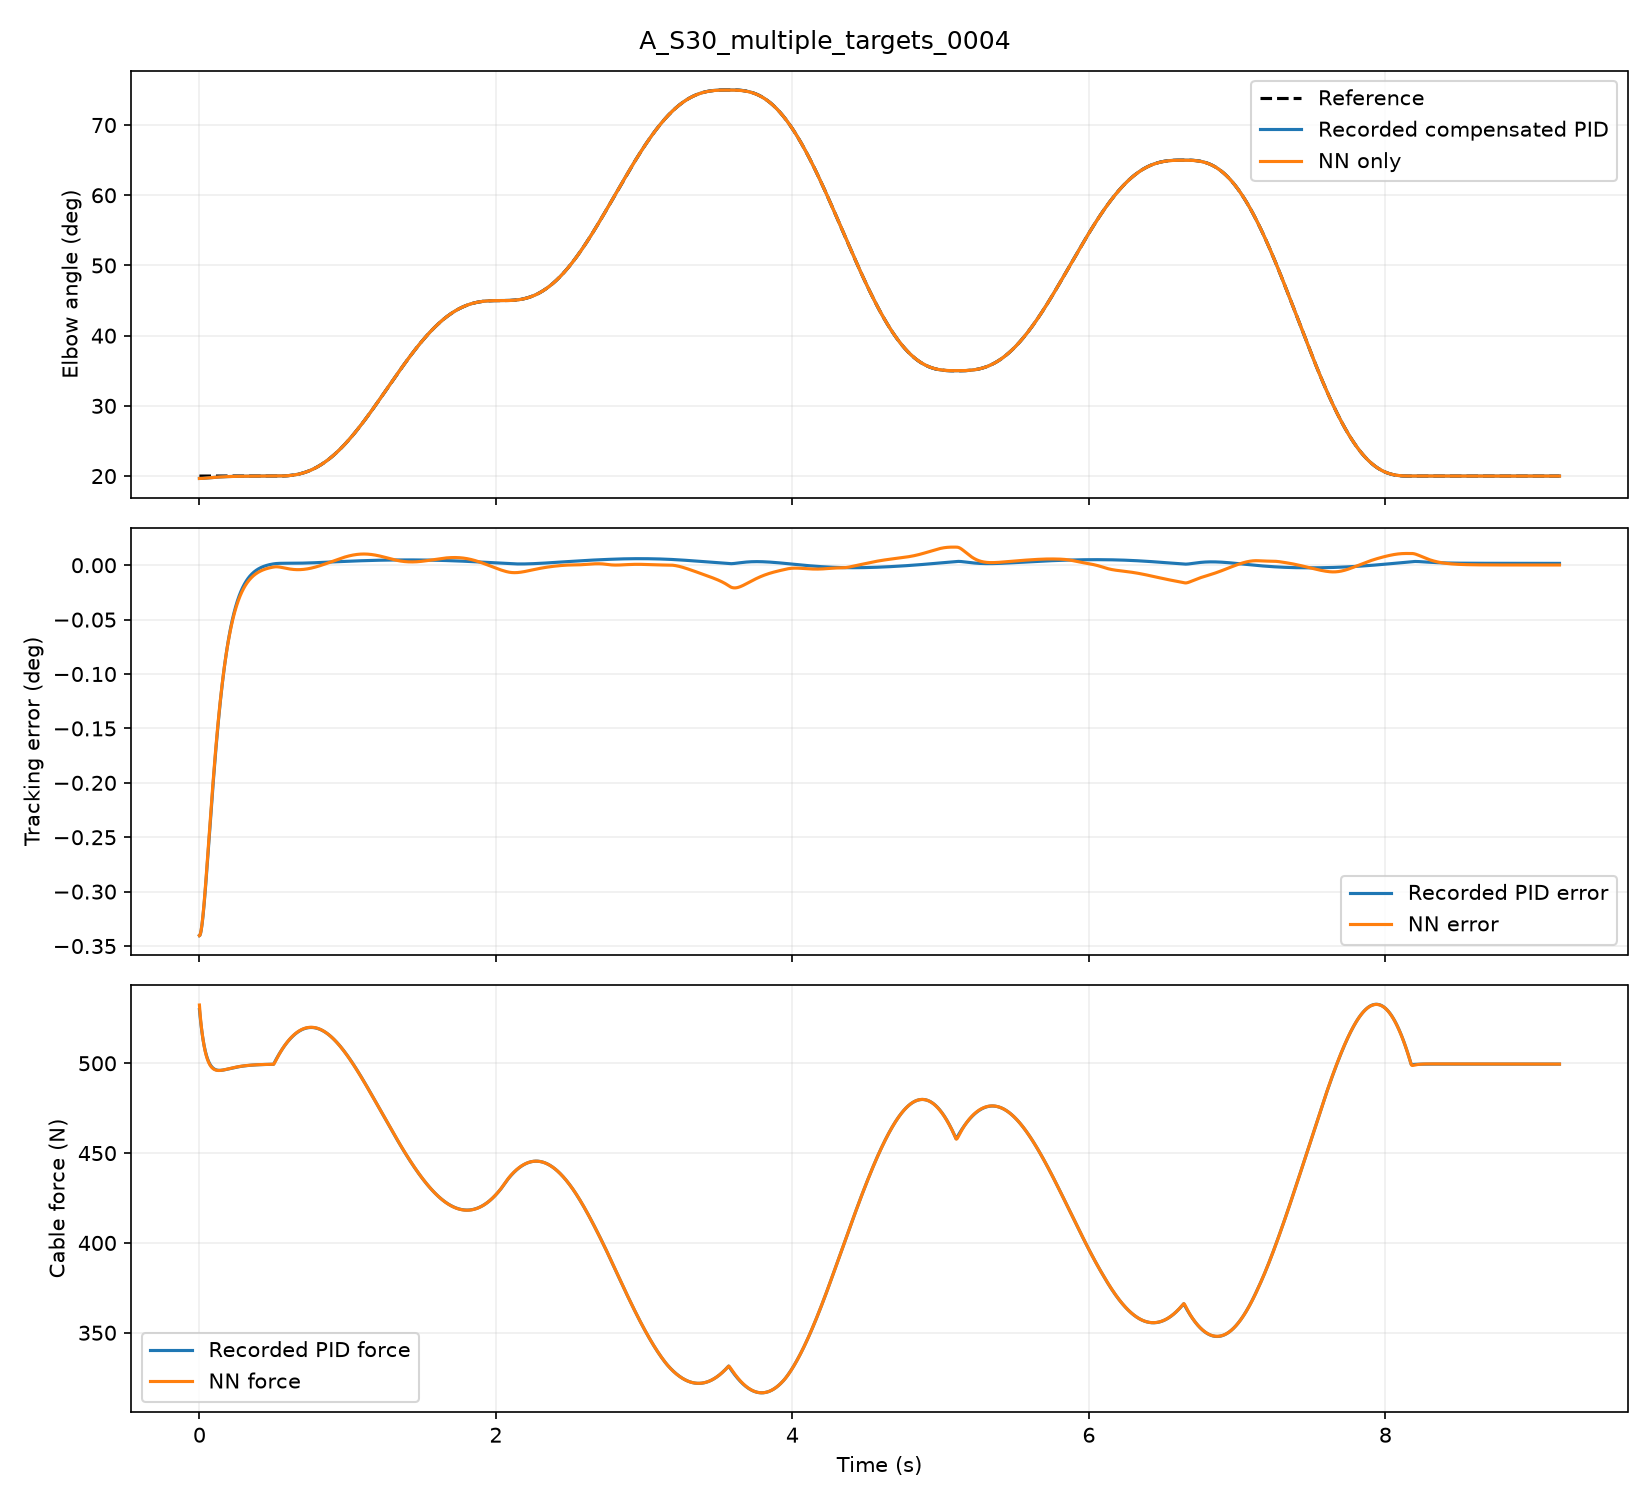
\includegraphics[width=\linewidth,height=0.69\textheight,keepaspectratio]{overleaf_figures/tracking_A_S30_multiple_targets_0004_comparison.png}
\caption{tracking/A\_S30\_multiple\_targets\_0004/comparison.png: Held-out OpenSim rollout: reference, recorded PID, and NN elbow motion; tracking errors; and cable forces. The NN supplies the cable command without a PID fallback.}
\label{fig:tracking_A_S30_multiple_targets_0004_comparison}
\end{figure}
\begin{figure}[H]\centering
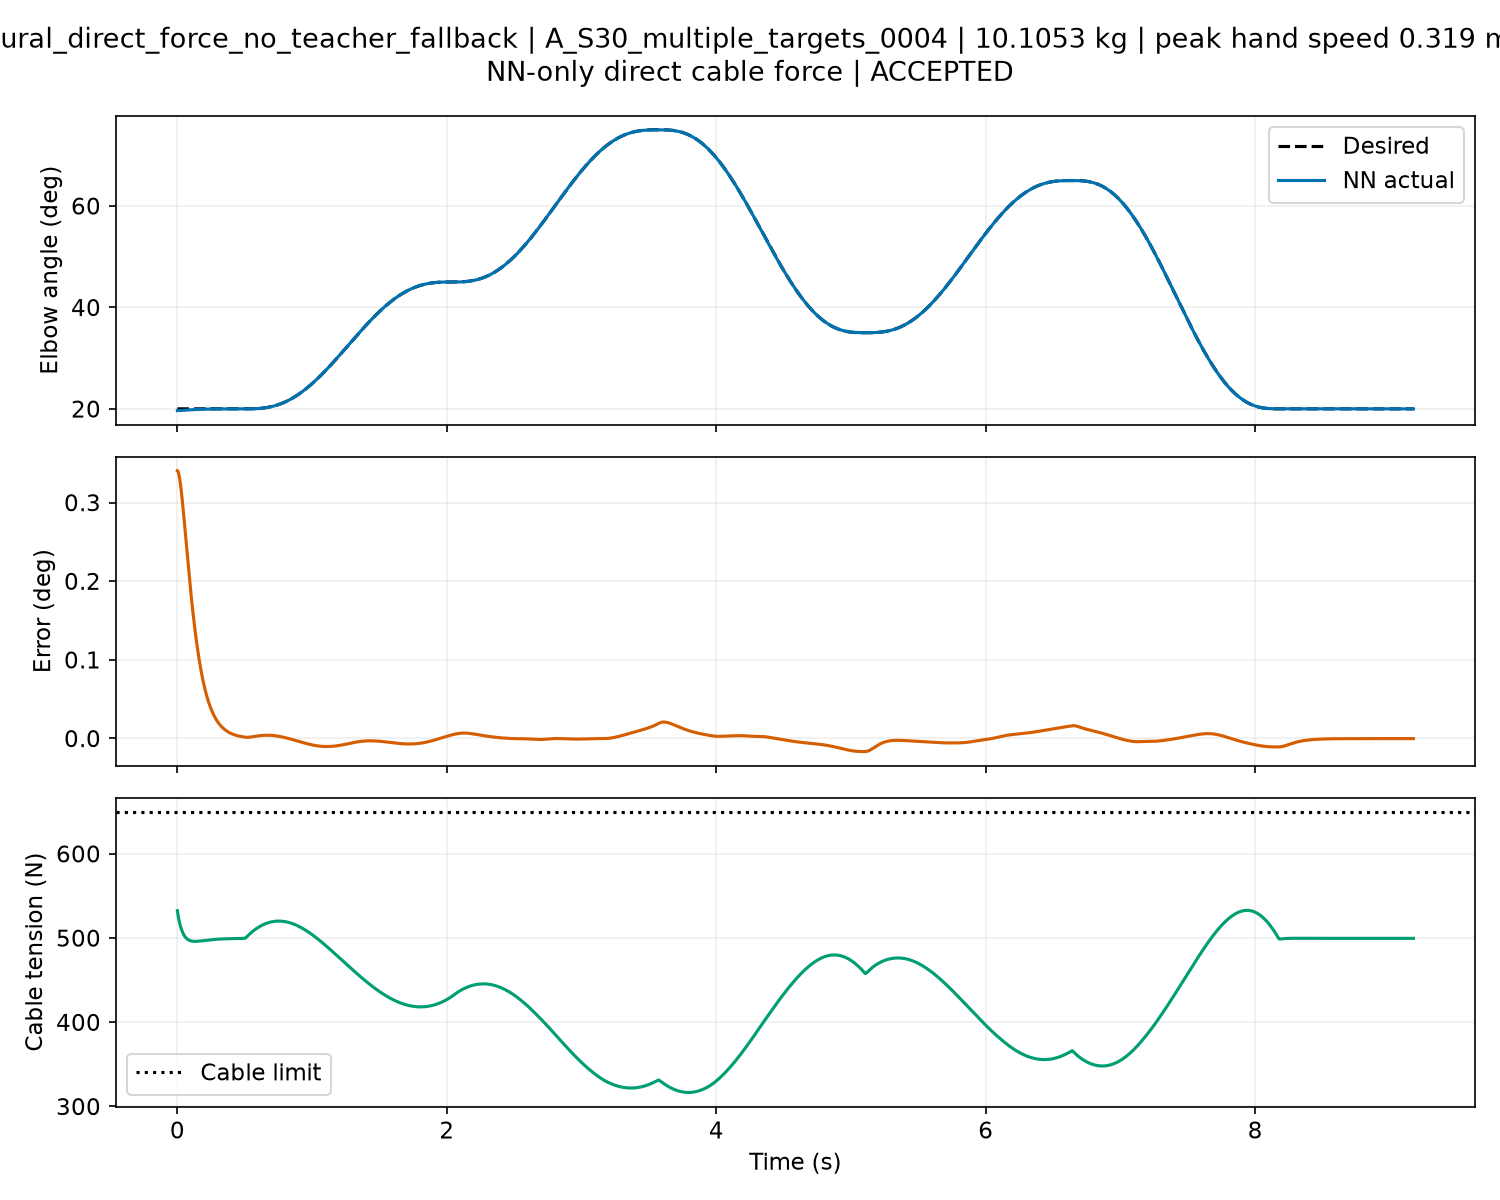
\includegraphics[width=\linewidth,height=0.69\textheight,keepaspectratio]{overleaf_figures/tracking_A_S30_multiple_targets_0004_tracking.png}
\caption{tracking/A\_S30\_multiple\_targets\_0004/tracking.png: Saved simulation diagnostics. Quantities and units are identified on the axes; failed runs are retained.}
\label{fig:tracking_A_S30_multiple_targets_0004_tracking}
\end{figure}
\begin{figure}[H]\centering
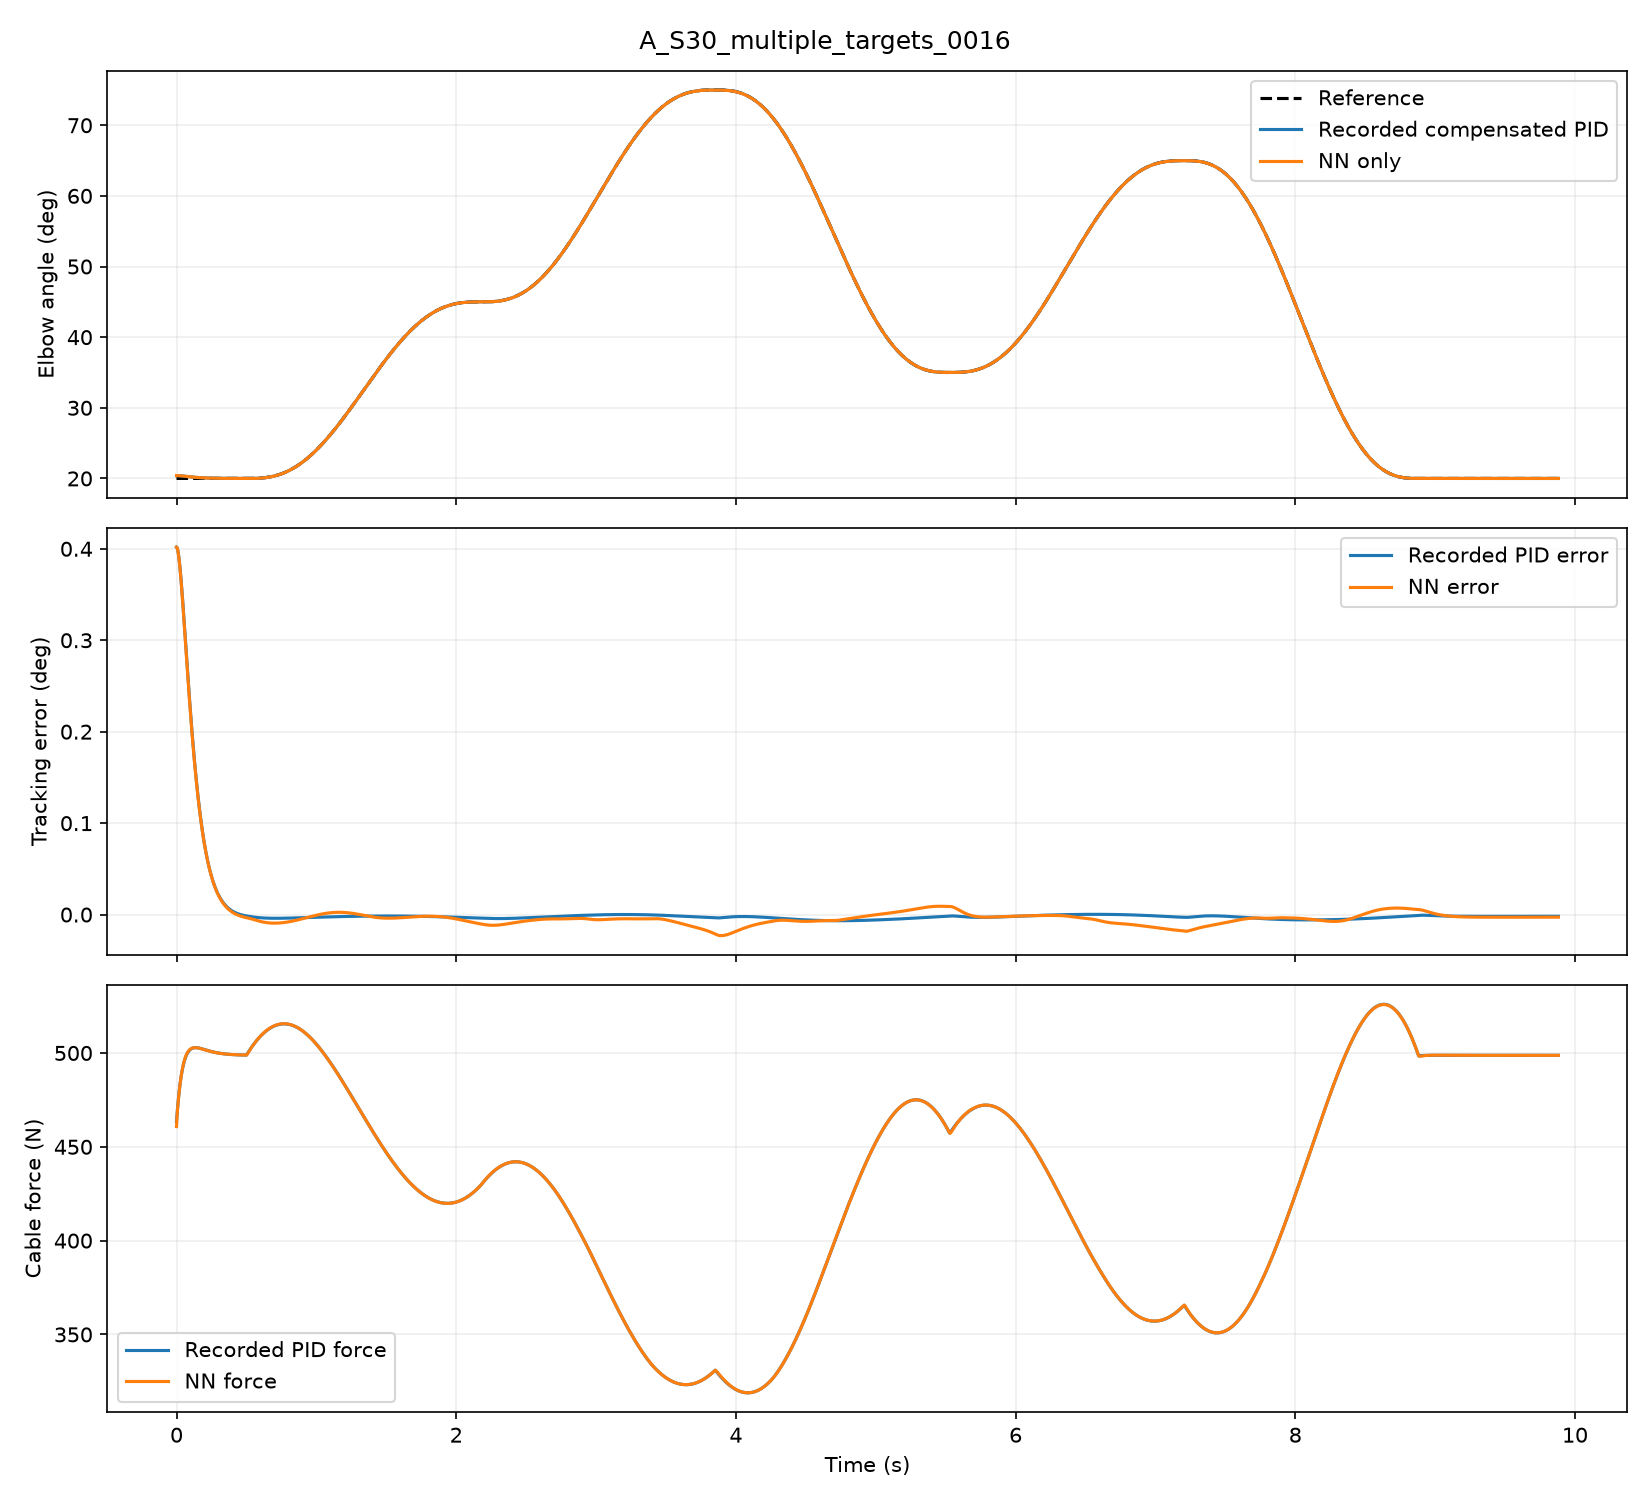
\includegraphics[width=\linewidth,height=0.69\textheight,keepaspectratio]{overleaf_figures/tracking_A_S30_multiple_targets_0016_comparison.png}
\caption{tracking/A\_S30\_multiple\_targets\_0016/comparison.png: Held-out OpenSim rollout: reference, recorded PID, and NN elbow motion; tracking errors; and cable forces. The NN supplies the cable command without a PID fallback.}
\label{fig:tracking_A_S30_multiple_targets_0016_comparison}
\end{figure}
\begin{figure}[H]\centering
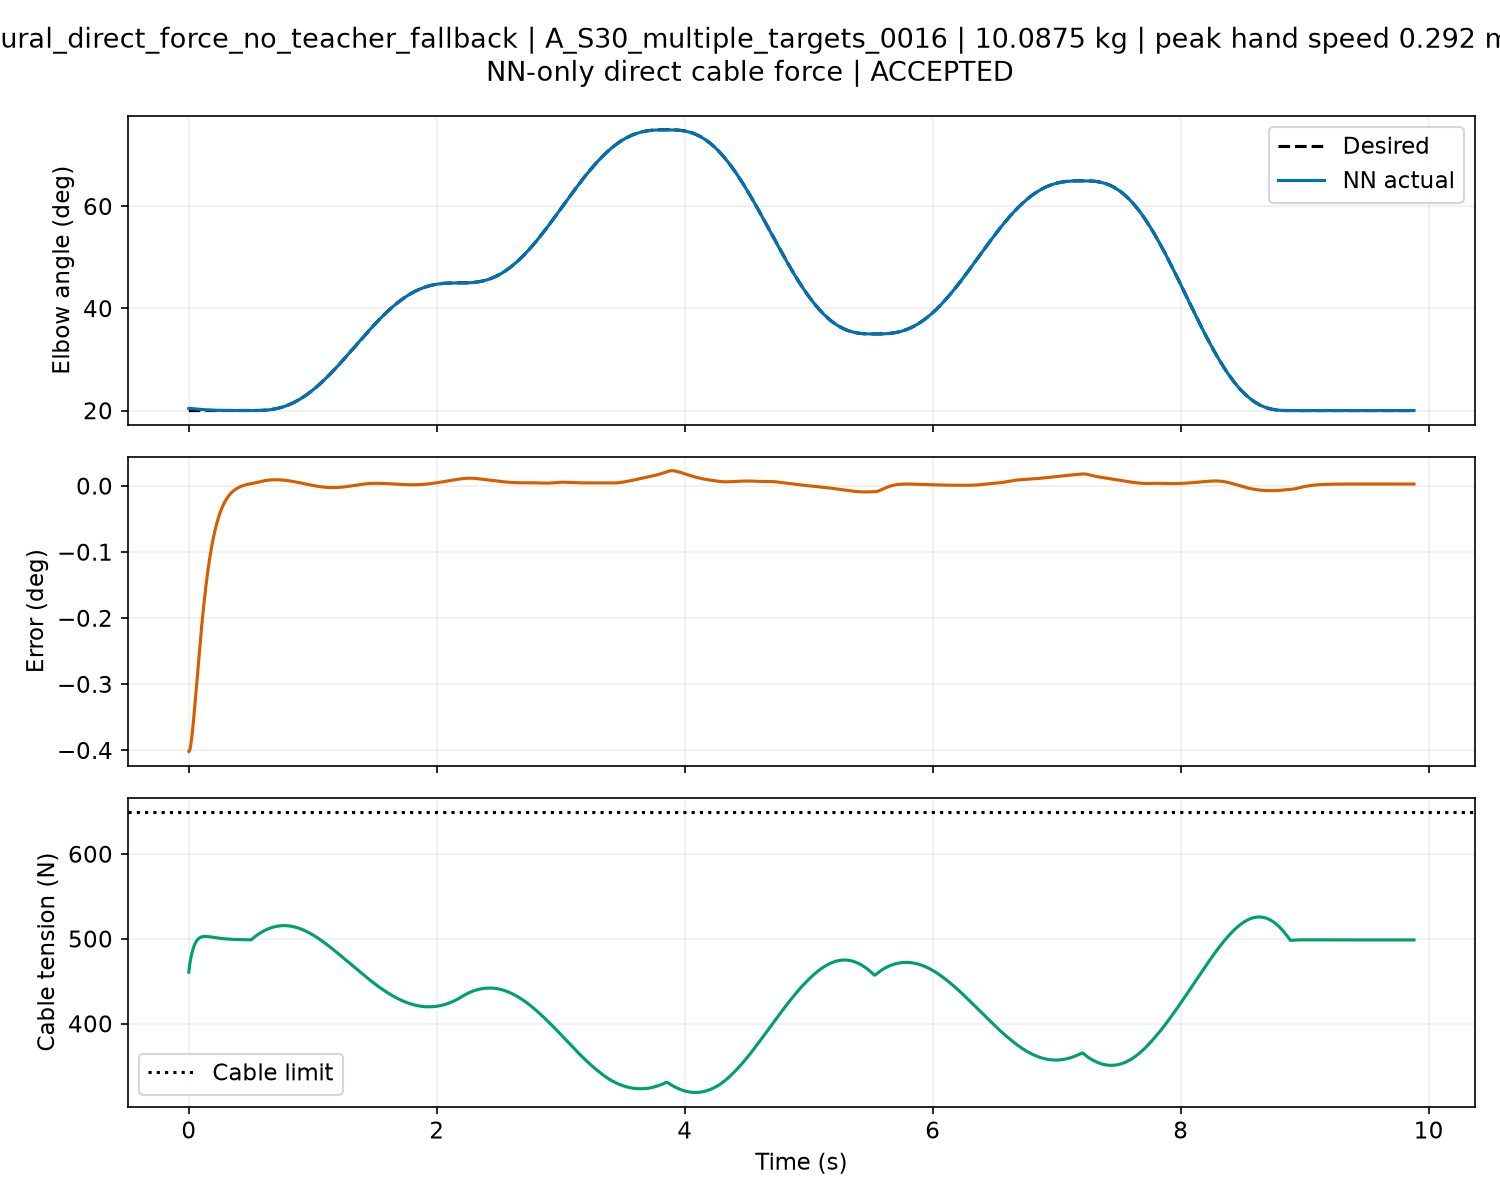
\includegraphics[width=\linewidth,height=0.69\textheight,keepaspectratio]{overleaf_figures/tracking_A_S30_multiple_targets_0016_tracking.png}
\caption{tracking/A\_S30\_multiple\_targets\_0016/tracking.png: Saved simulation diagnostics. Quantities and units are identified on the axes; failed runs are retained.}
\label{fig:tracking_A_S30_multiple_targets_0016_tracking}
\end{figure}
\begin{figure}[H]\centering
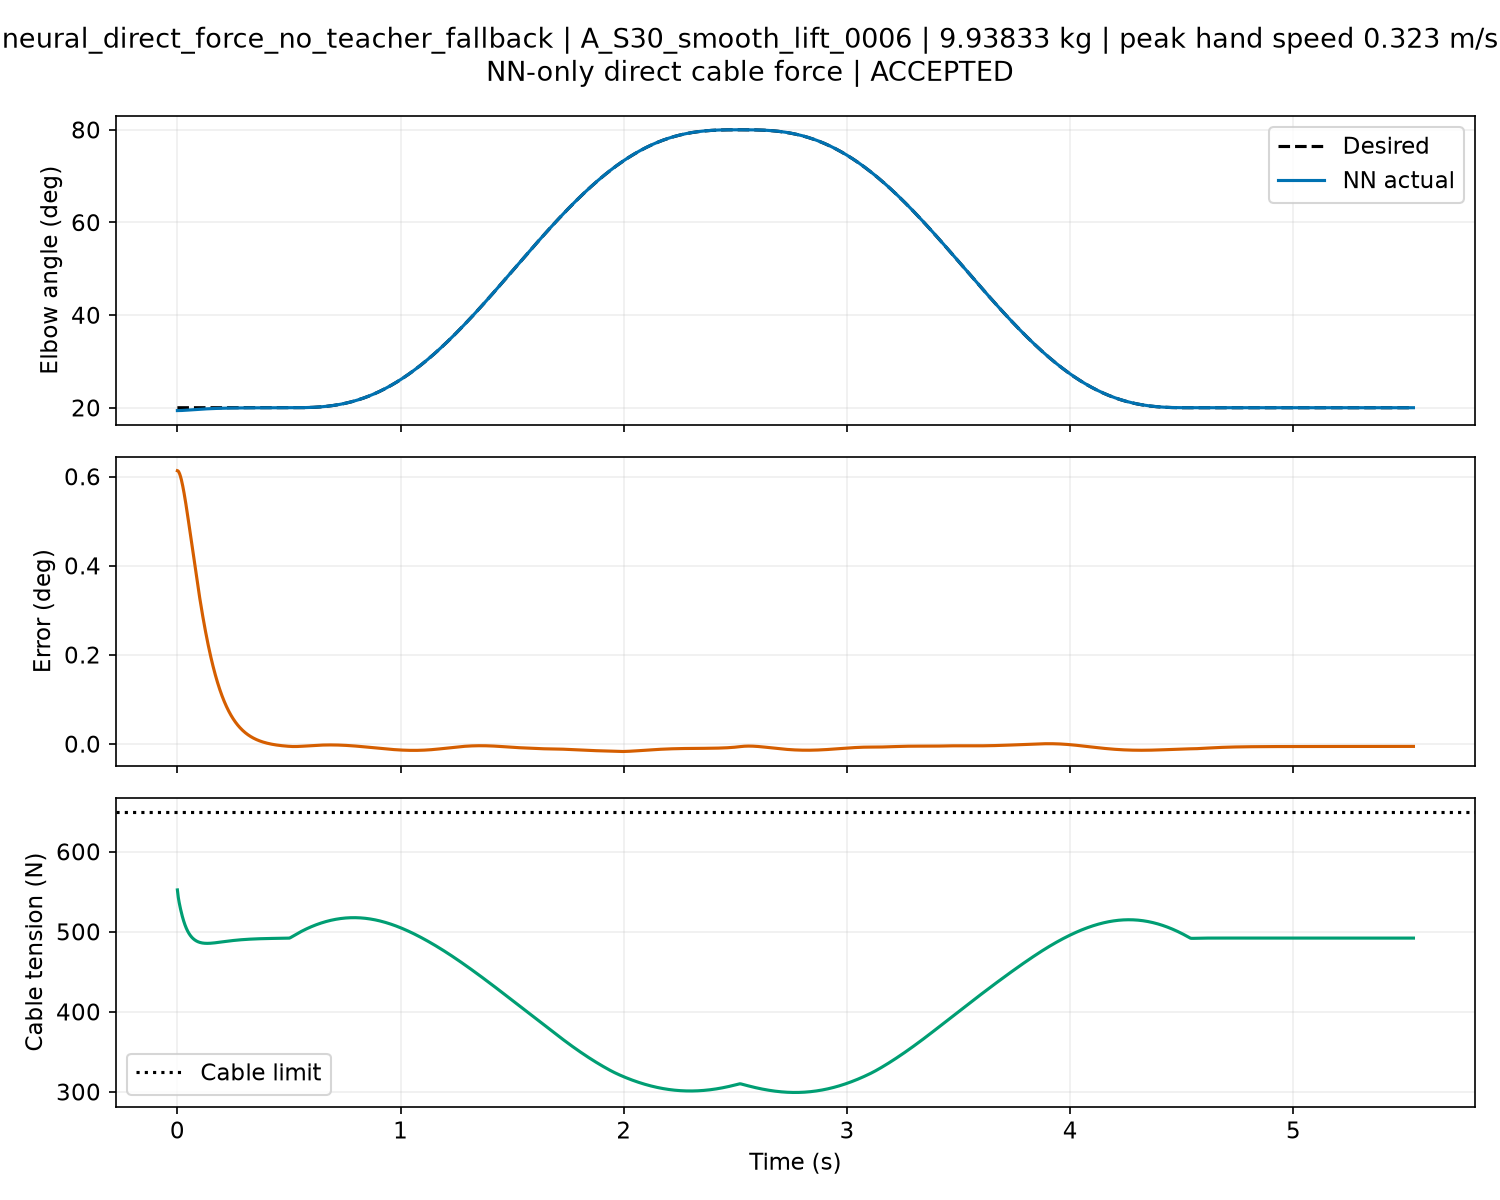
\includegraphics[width=\linewidth,height=0.69\textheight,keepaspectratio]{overleaf_figures/tracking_A_S30_smooth_lift_0006_tracking.png}
\caption{tracking/A\_S30\_smooth\_lift\_0006/tracking.png: Saved simulation diagnostics. Quantities and units are identified on the axes; failed runs are retained.}
\label{fig:tracking_A_S30_smooth_lift_0006_tracking}
\end{figure}
\begin{figure}[H]\centering
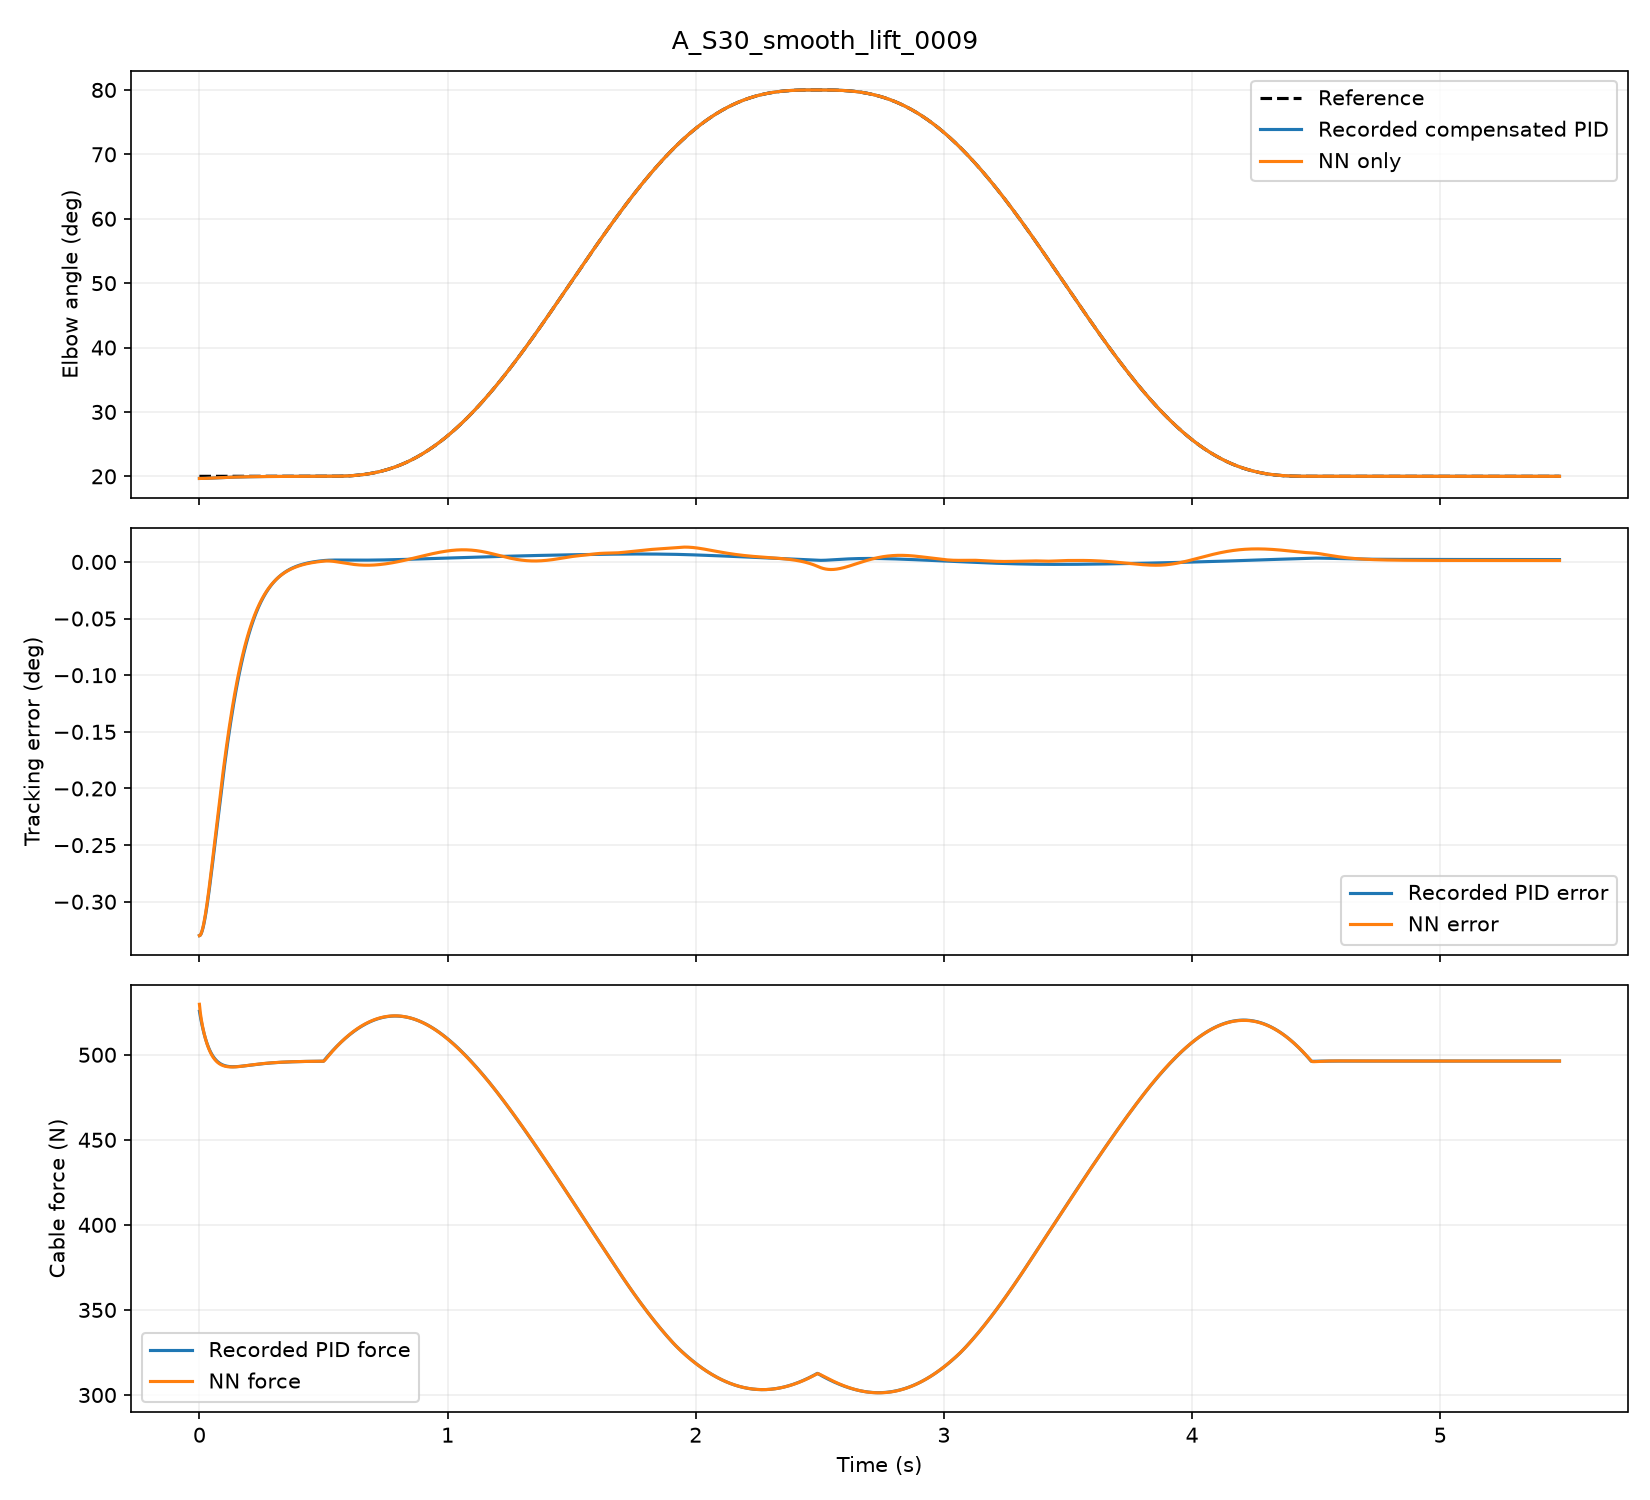
\includegraphics[width=\linewidth,height=0.69\textheight,keepaspectratio]{overleaf_figures/tracking_A_S30_smooth_lift_0009_comparison.png}
\caption{tracking/A\_S30\_smooth\_lift\_0009/comparison.png: Held-out OpenSim rollout: reference, recorded PID, and NN elbow motion; tracking errors; and cable forces. The NN supplies the cable command without a PID fallback.}
\label{fig:tracking_A_S30_smooth_lift_0009_comparison}
\end{figure}
\begin{figure}[H]\centering
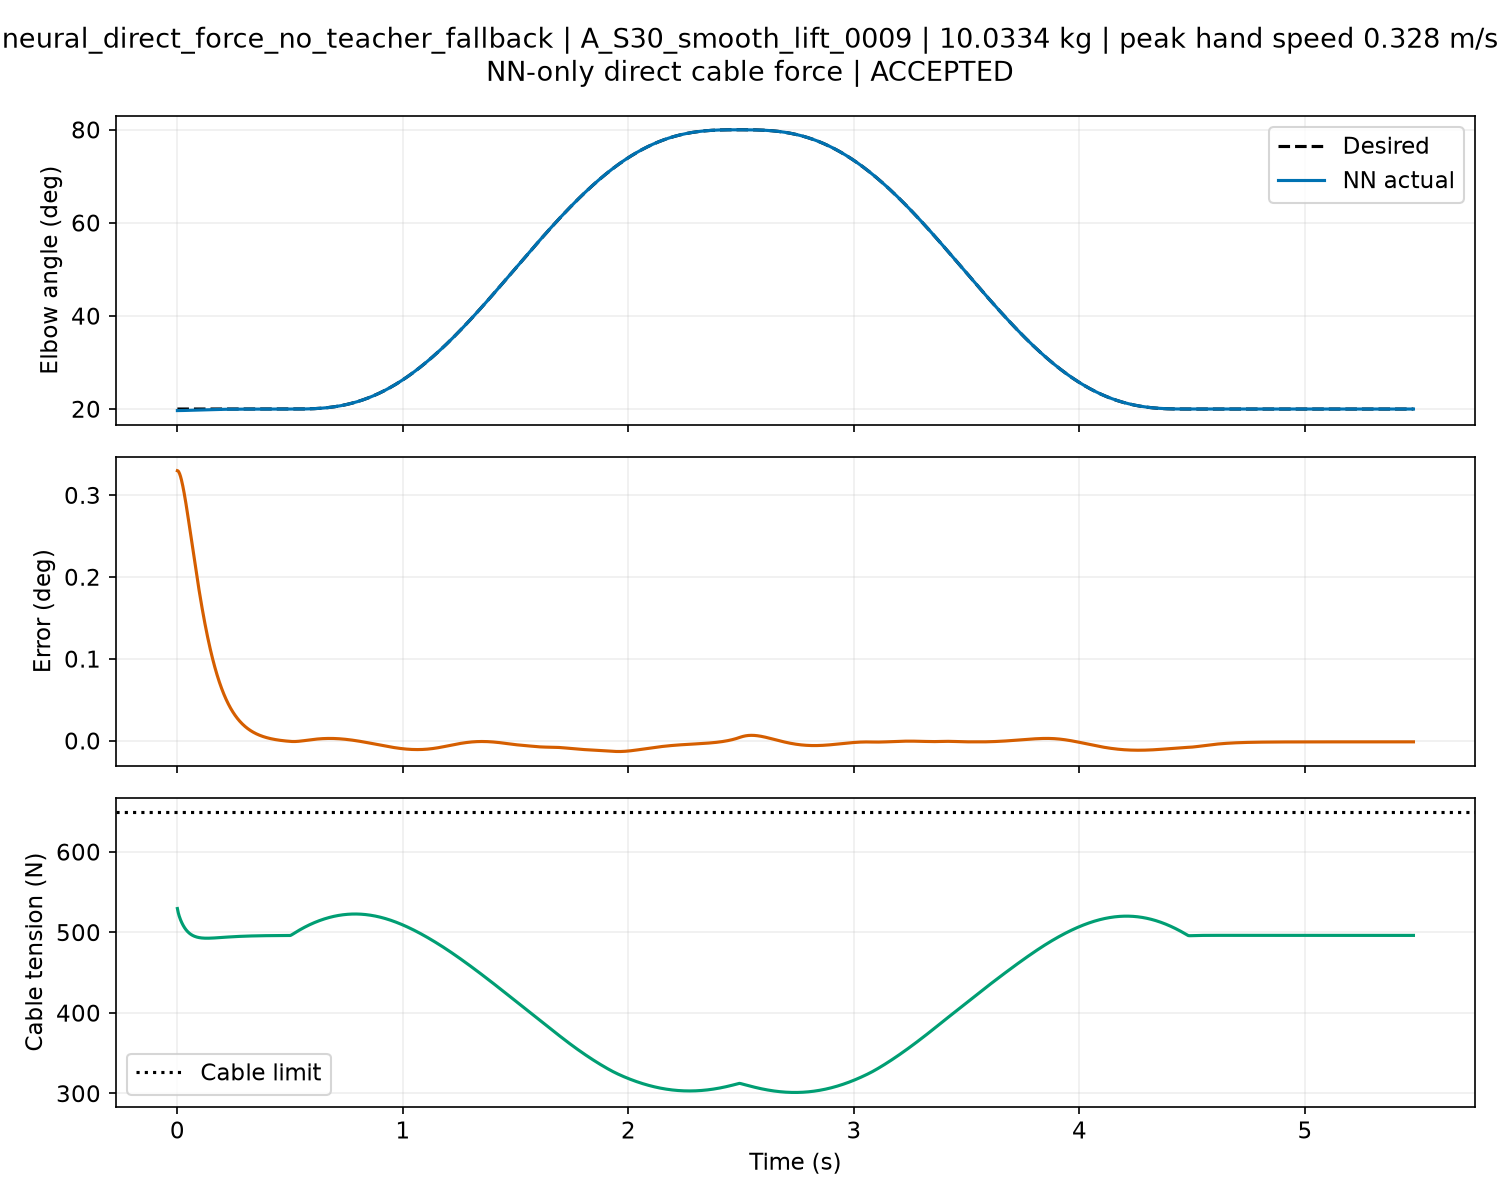
\includegraphics[width=\linewidth,height=0.69\textheight,keepaspectratio]{overleaf_figures/tracking_A_S30_smooth_lift_0009_tracking.png}
\caption{tracking/A\_S30\_smooth\_lift\_0009/tracking.png: Saved simulation diagnostics. Quantities and units are identified on the axes; failed runs are retained.}
\label{fig:tracking_A_S30_smooth_lift_0009_tracking}
\end{figure}
\begin{figure}[H]\centering
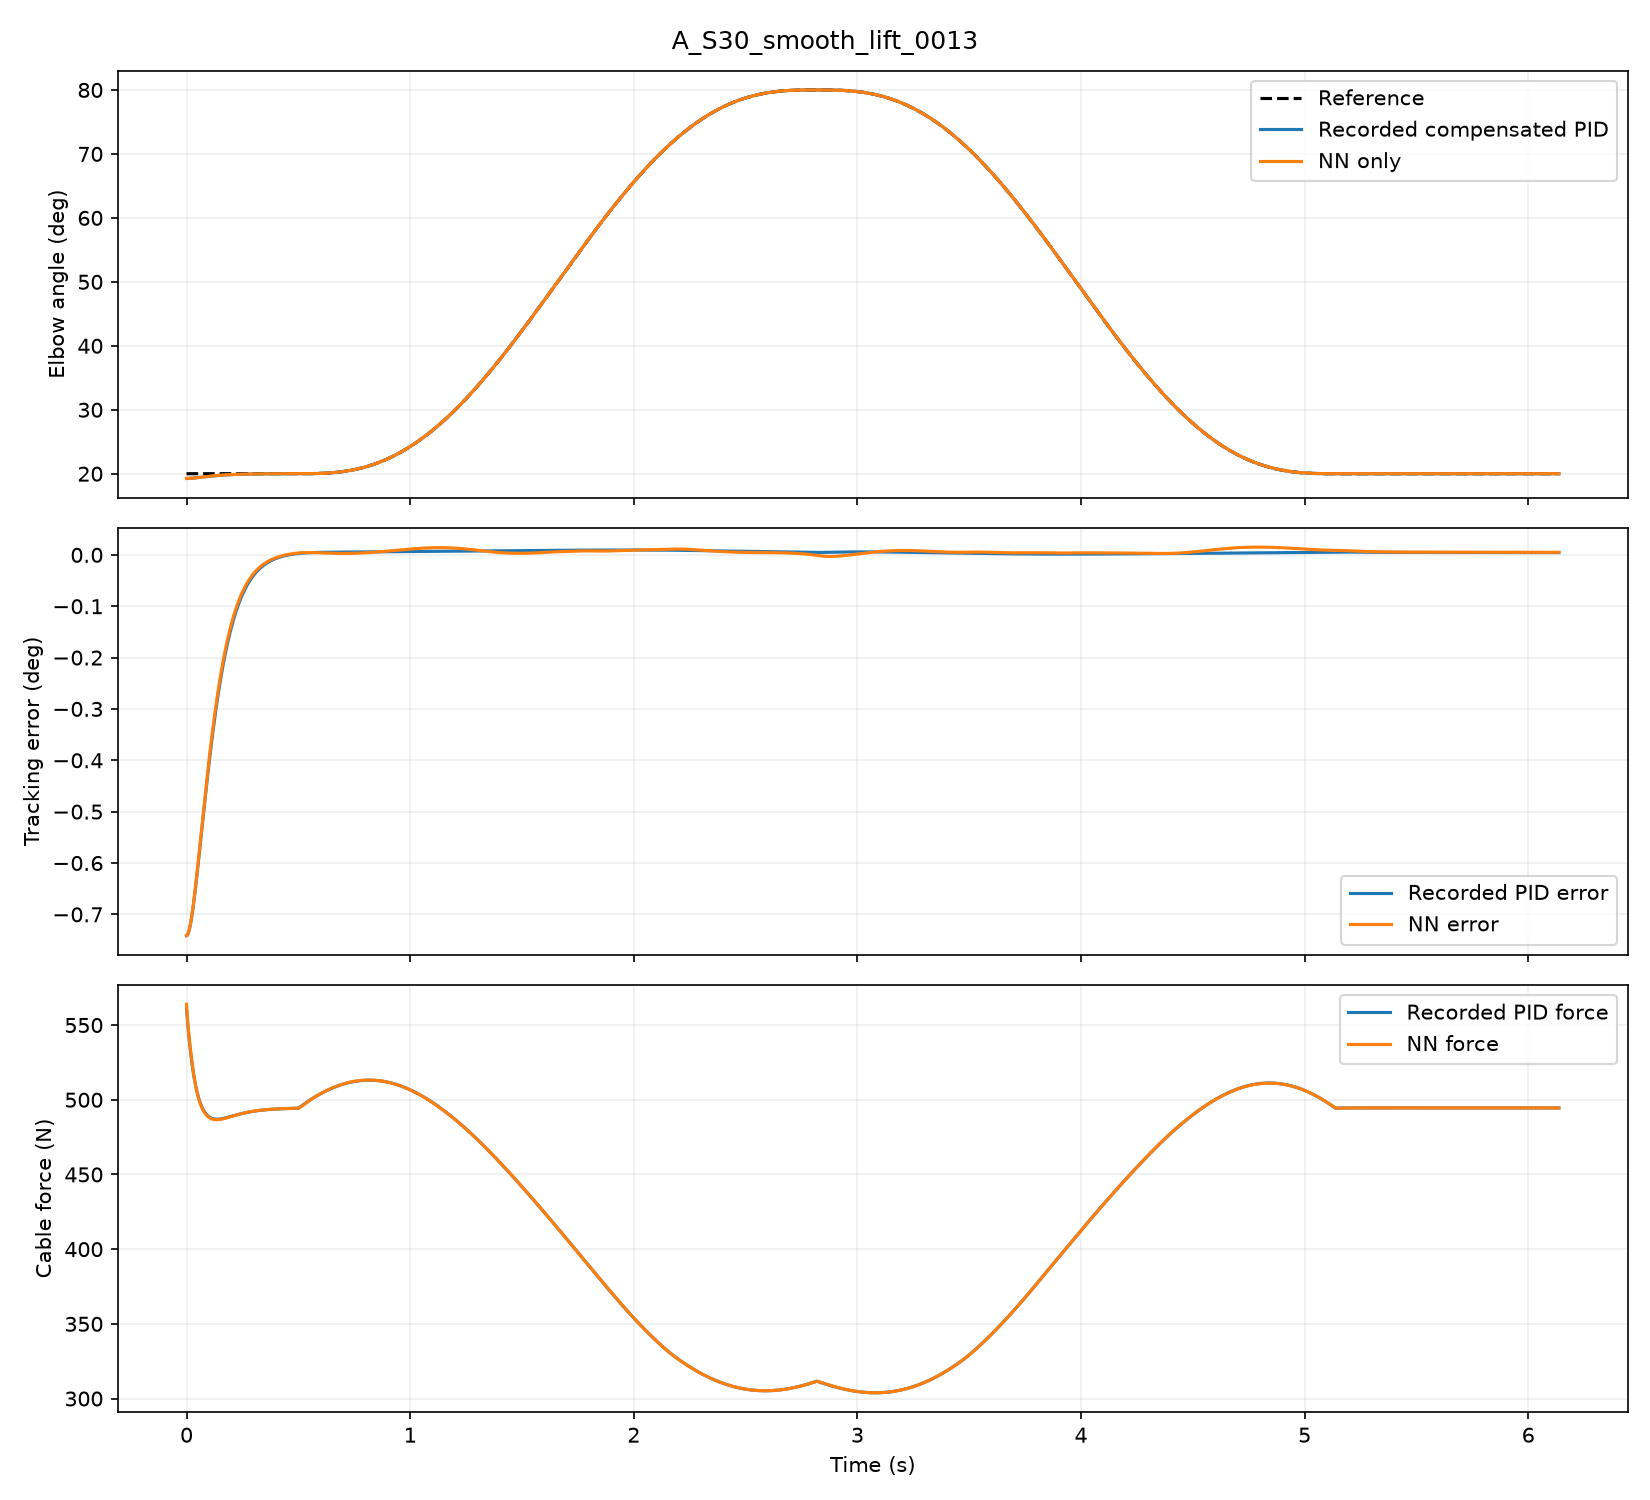
\includegraphics[width=\linewidth,height=0.69\textheight,keepaspectratio]{overleaf_figures/tracking_A_S30_smooth_lift_0013_comparison.png}
\caption{tracking/A\_S30\_smooth\_lift\_0013/comparison.png: Held-out OpenSim rollout: reference, recorded PID, and NN elbow motion; tracking errors; and cable forces. The NN supplies the cable command without a PID fallback.}
\label{fig:tracking_A_S30_smooth_lift_0013_comparison}
\end{figure}
\begin{figure}[H]\centering
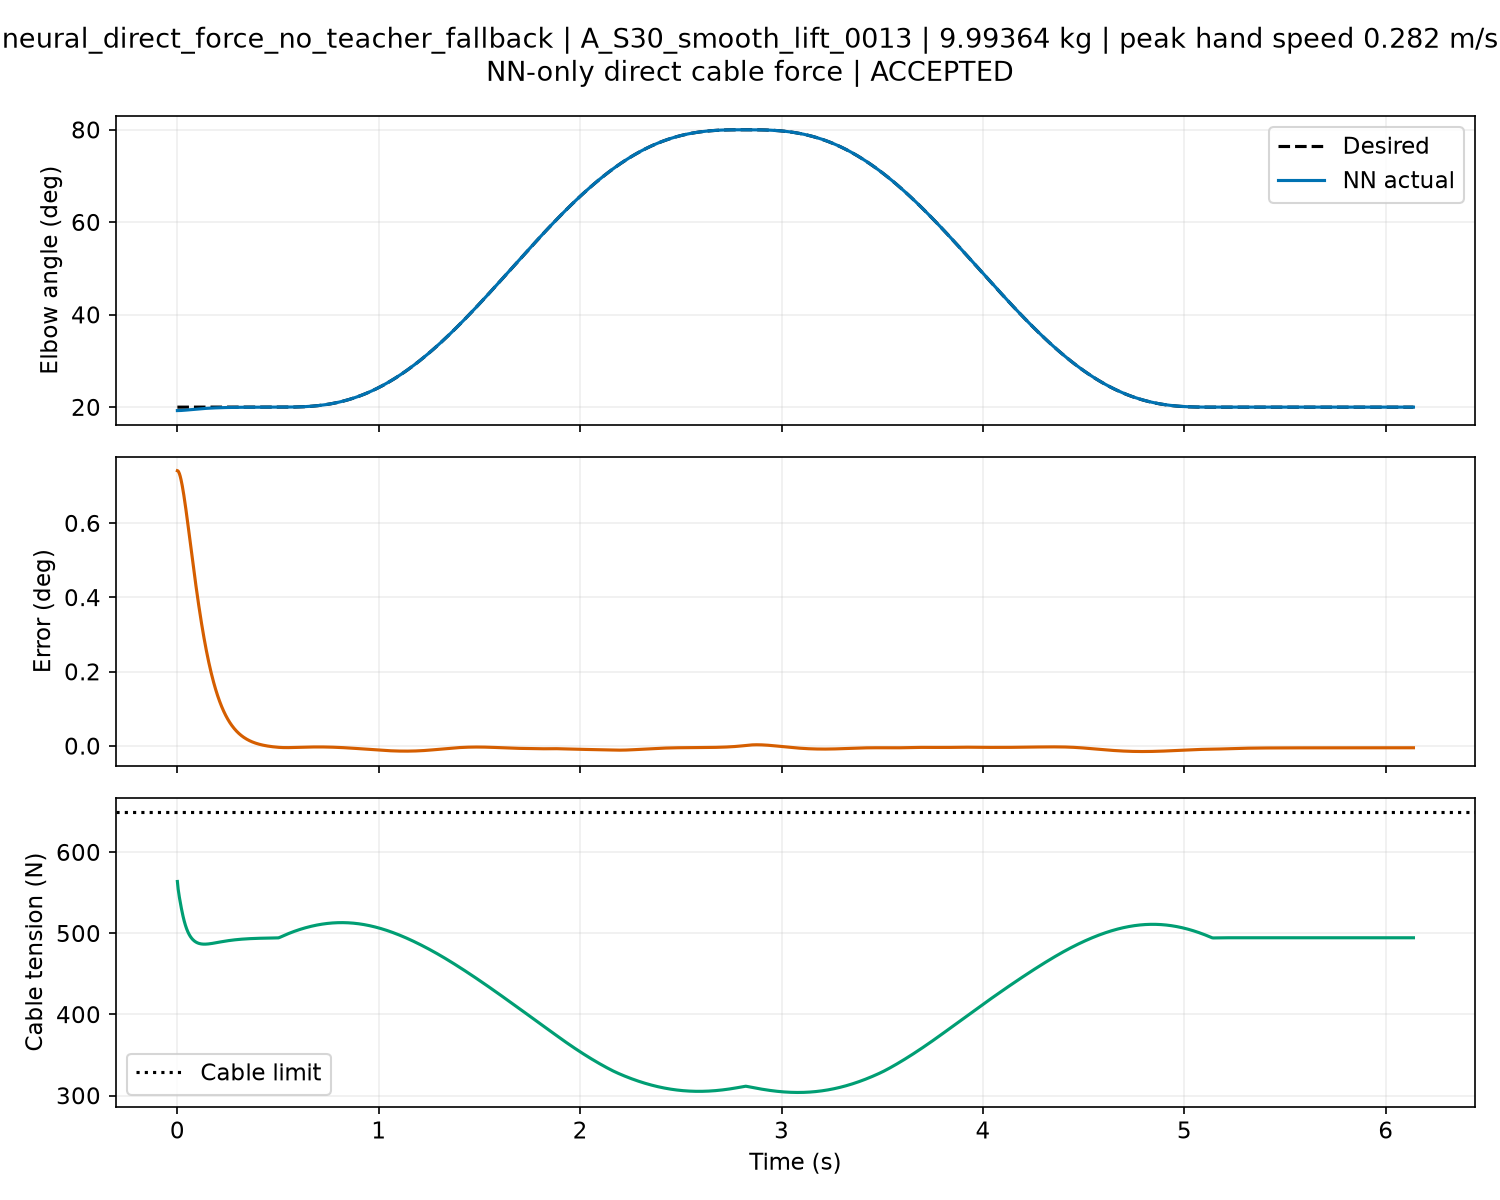
\includegraphics[width=\linewidth,height=0.69\textheight,keepaspectratio]{overleaf_figures/tracking_A_S30_smooth_lift_0013_tracking.png}
\caption{tracking/A\_S30\_smooth\_lift\_0013/tracking.png: Saved simulation diagnostics. Quantities and units are identified on the axes; failed runs are retained.}
\label{fig:tracking_A_S30_smooth_lift_0013_tracking}
\end{figure}
\begin{figure}[H]\centering
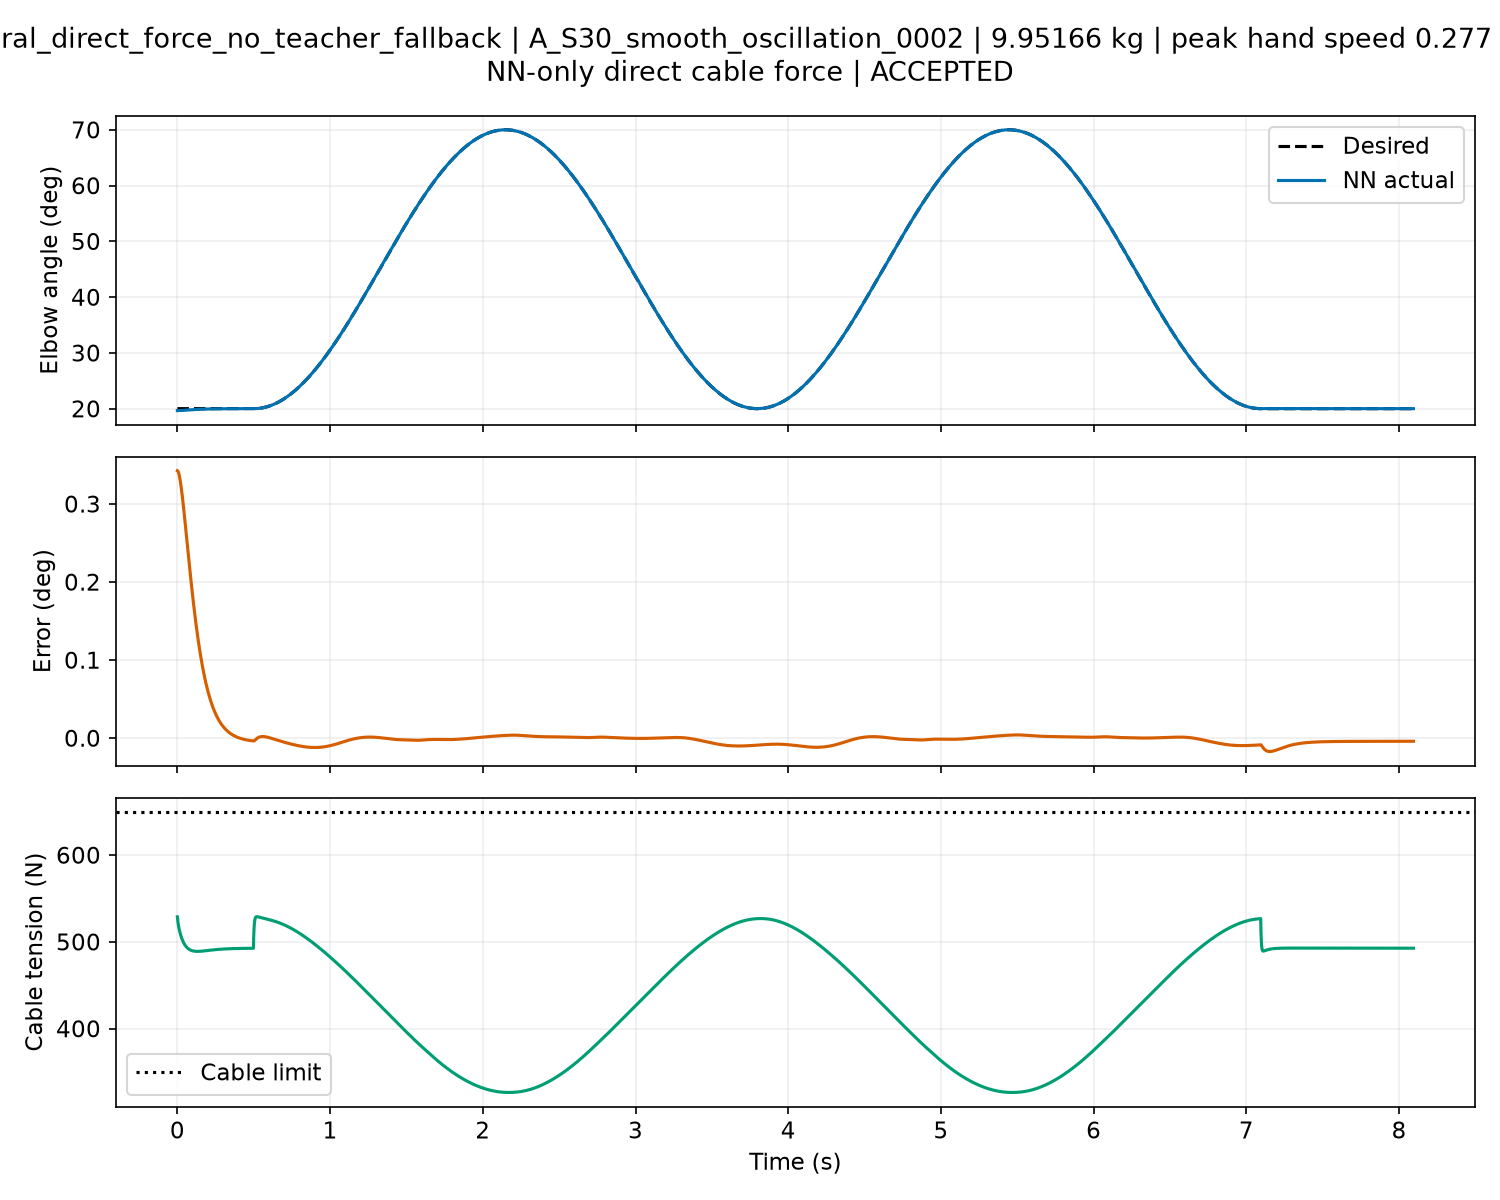
\includegraphics[width=\linewidth,height=0.69\textheight,keepaspectratio]{overleaf_figures/tracking_A_S30_smooth_oscillation_0002_tracking.png}
\caption{tracking/A\_S30\_smooth\_oscillation\_0002/tracking.png: Saved simulation diagnostics. Quantities and units are identified on the axes; failed runs are retained.}
\label{fig:tracking_A_S30_smooth_oscillation_0002_tracking}
\end{figure}
\begin{figure}[H]\centering
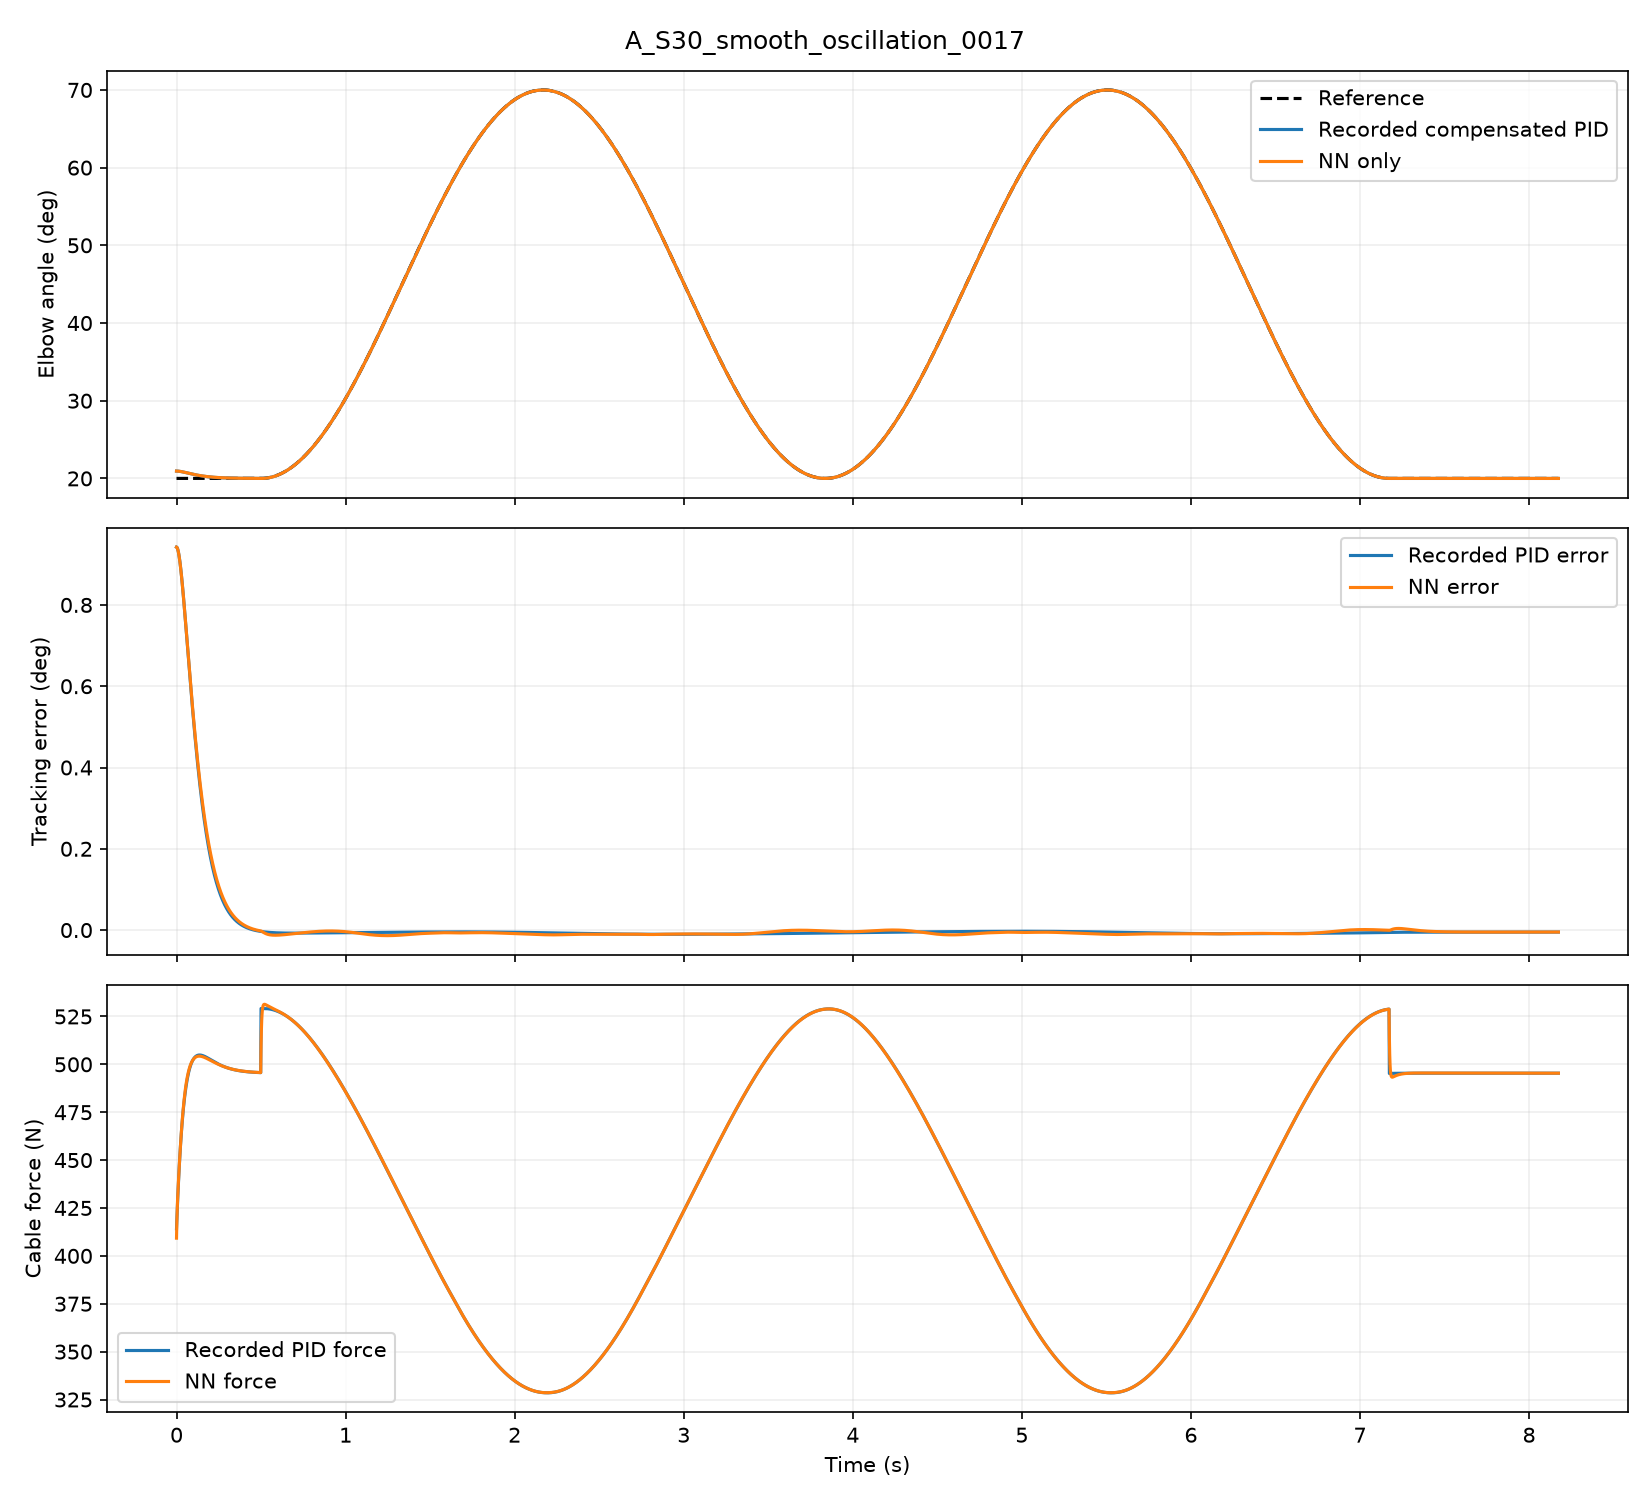
\includegraphics[width=\linewidth,height=0.69\textheight,keepaspectratio]{overleaf_figures/tracking_A_S30_smooth_oscillation_0017_comparison.png}
\caption{tracking/A\_S30\_smooth\_oscillation\_0017/comparison.png: Held-out OpenSim rollout: reference, recorded PID, and NN elbow motion; tracking errors; and cable forces. The NN supplies the cable command without a PID fallback.}
\label{fig:tracking_A_S30_smooth_oscillation_0017_comparison}
\end{figure}
\begin{figure}[H]\centering
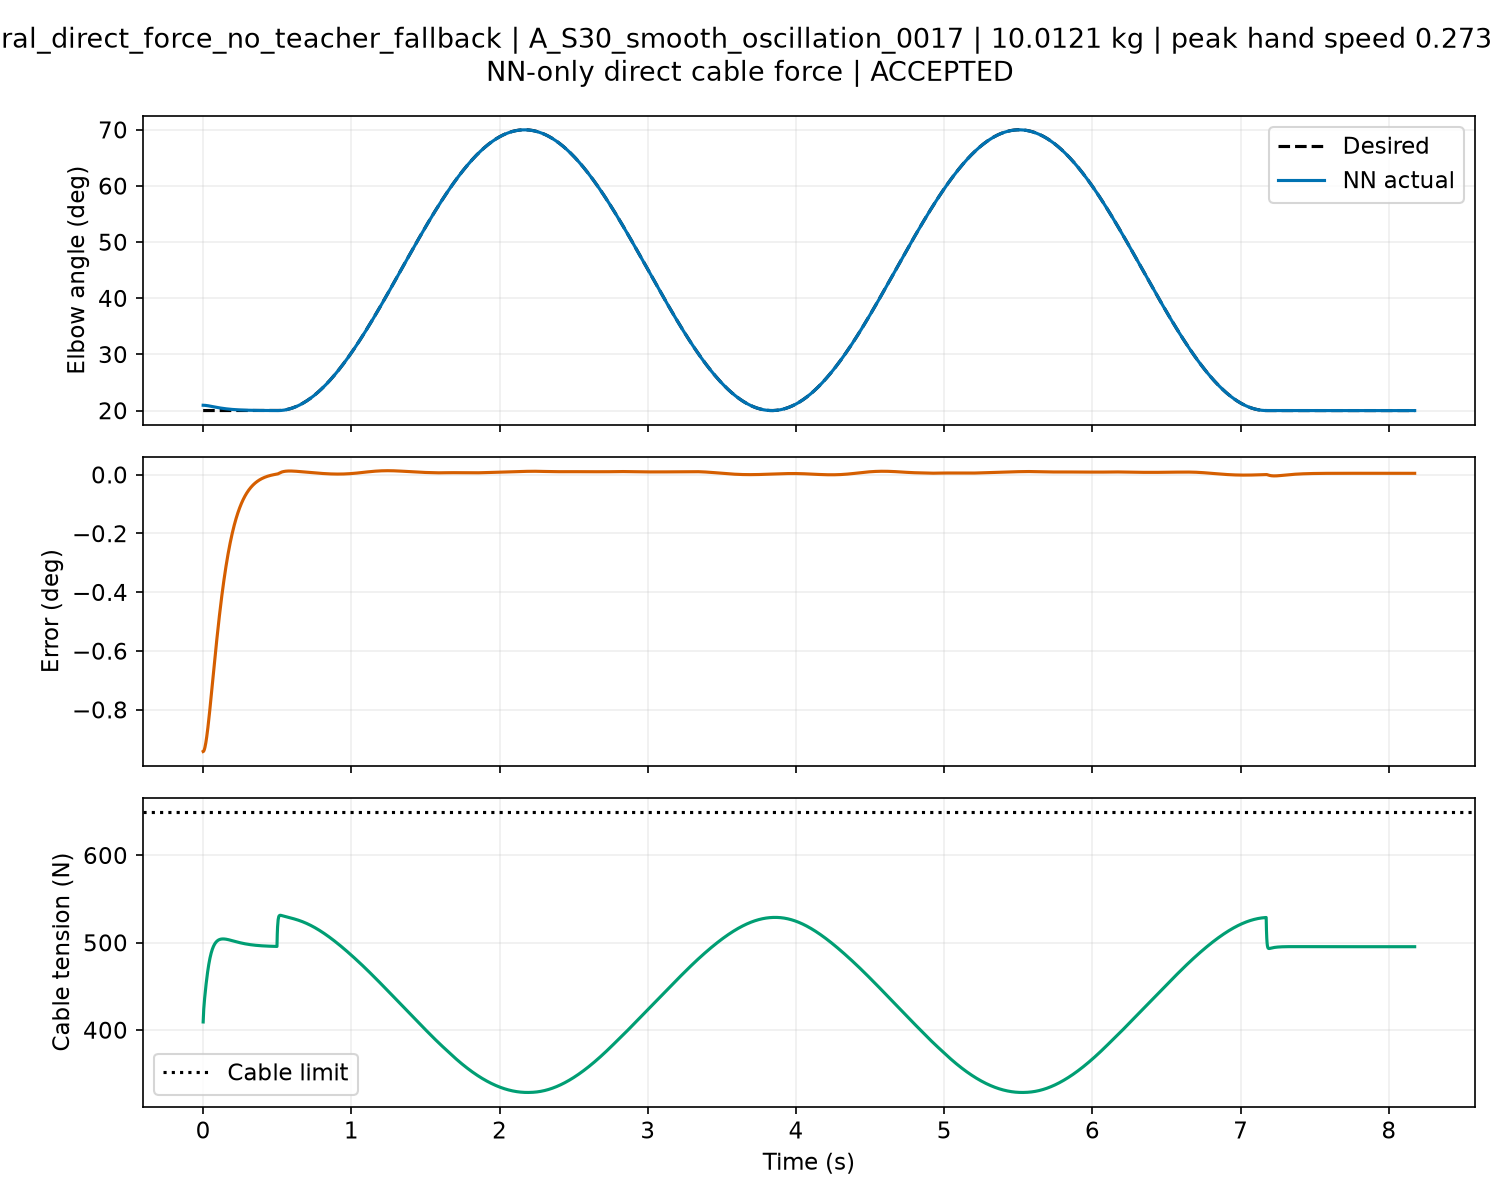
\includegraphics[width=\linewidth,height=0.69\textheight,keepaspectratio]{overleaf_figures/tracking_A_S30_smooth_oscillation_0017_tracking.png}
\caption{tracking/A\_S30\_smooth\_oscillation\_0017/tracking.png: Saved simulation diagnostics. Quantities and units are identified on the axes; failed runs are retained.}
\label{fig:tracking_A_S30_smooth_oscillation_0017_tracking}
\end{figure}
\begin{figure}[H]\centering
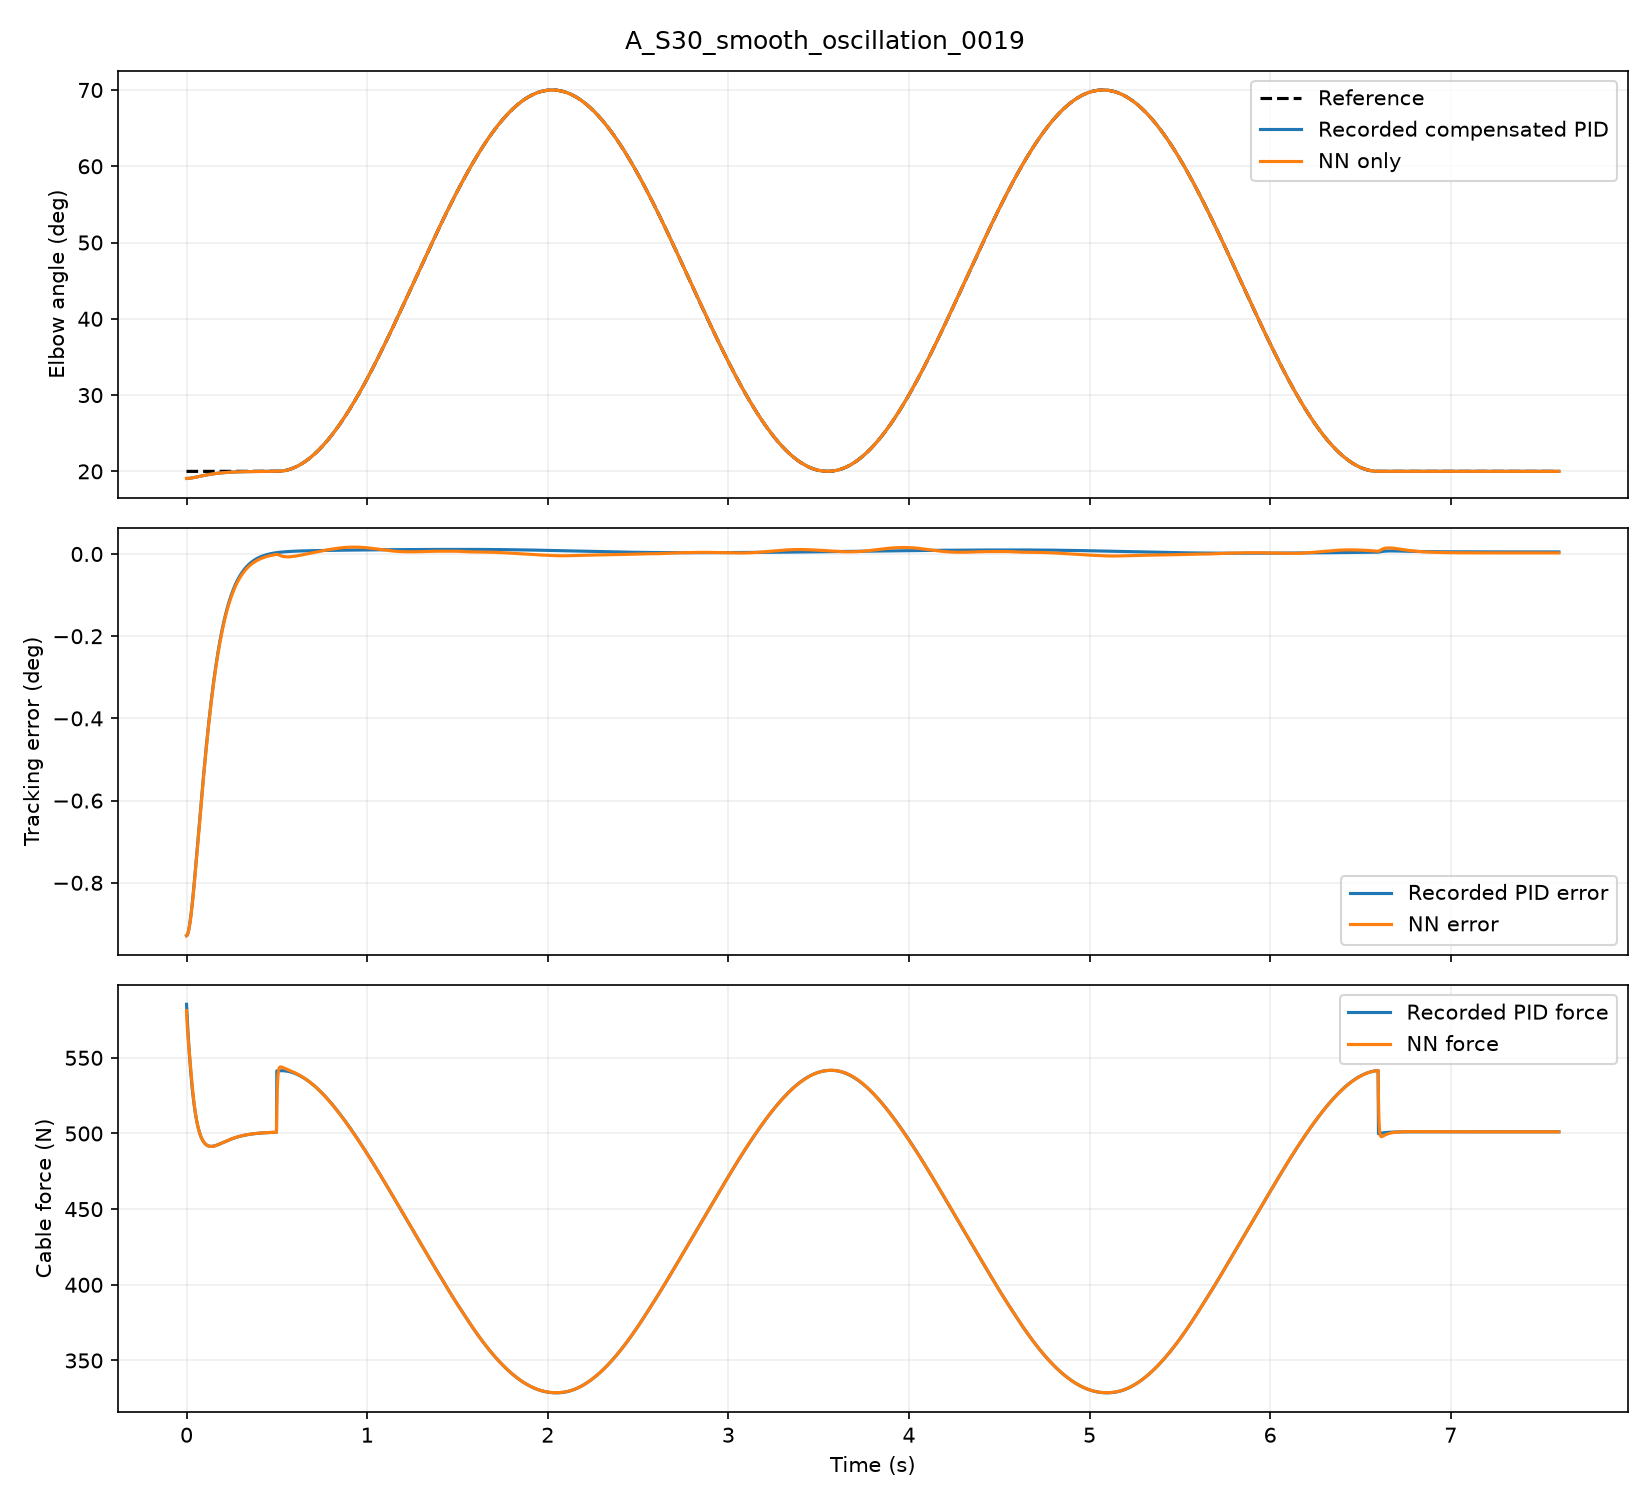
\includegraphics[width=\linewidth,height=0.69\textheight,keepaspectratio]{overleaf_figures/tracking_A_S30_smooth_oscillation_0019_comparison.png}
\caption{tracking/A\_S30\_smooth\_oscillation\_0019/comparison.png: Held-out OpenSim rollout: reference, recorded PID, and NN elbow motion; tracking errors; and cable forces. The NN supplies the cable command without a PID fallback.}
\label{fig:tracking_A_S30_smooth_oscillation_0019_comparison}
\end{figure}
\begin{figure}[H]\centering
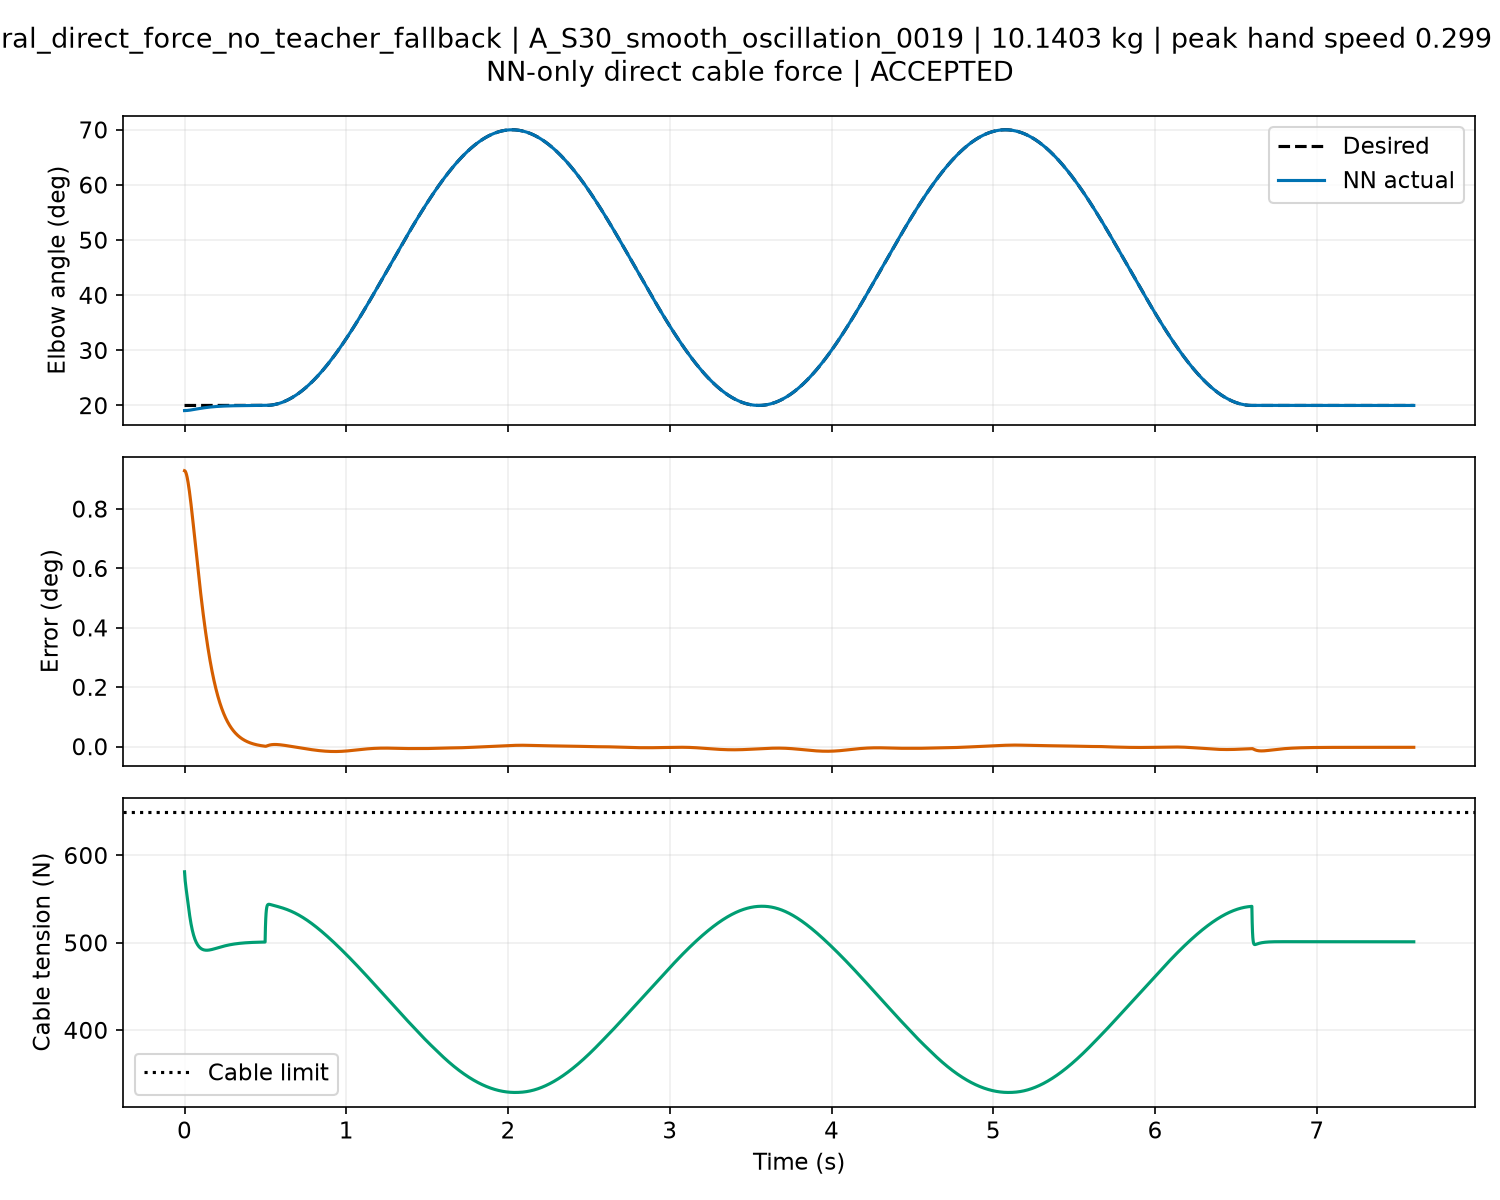
\includegraphics[width=\linewidth,height=0.69\textheight,keepaspectratio]{overleaf_figures/tracking_A_S30_smooth_oscillation_0019_tracking.png}
\caption{tracking/A\_S30\_smooth\_oscillation\_0019/tracking.png: Saved simulation diagnostics. Quantities and units are identified on the axes; failed runs are retained.}
\label{fig:tracking_A_S30_smooth_oscillation_0019_tracking}
\end{figure}
\begin{figure}[H]\centering
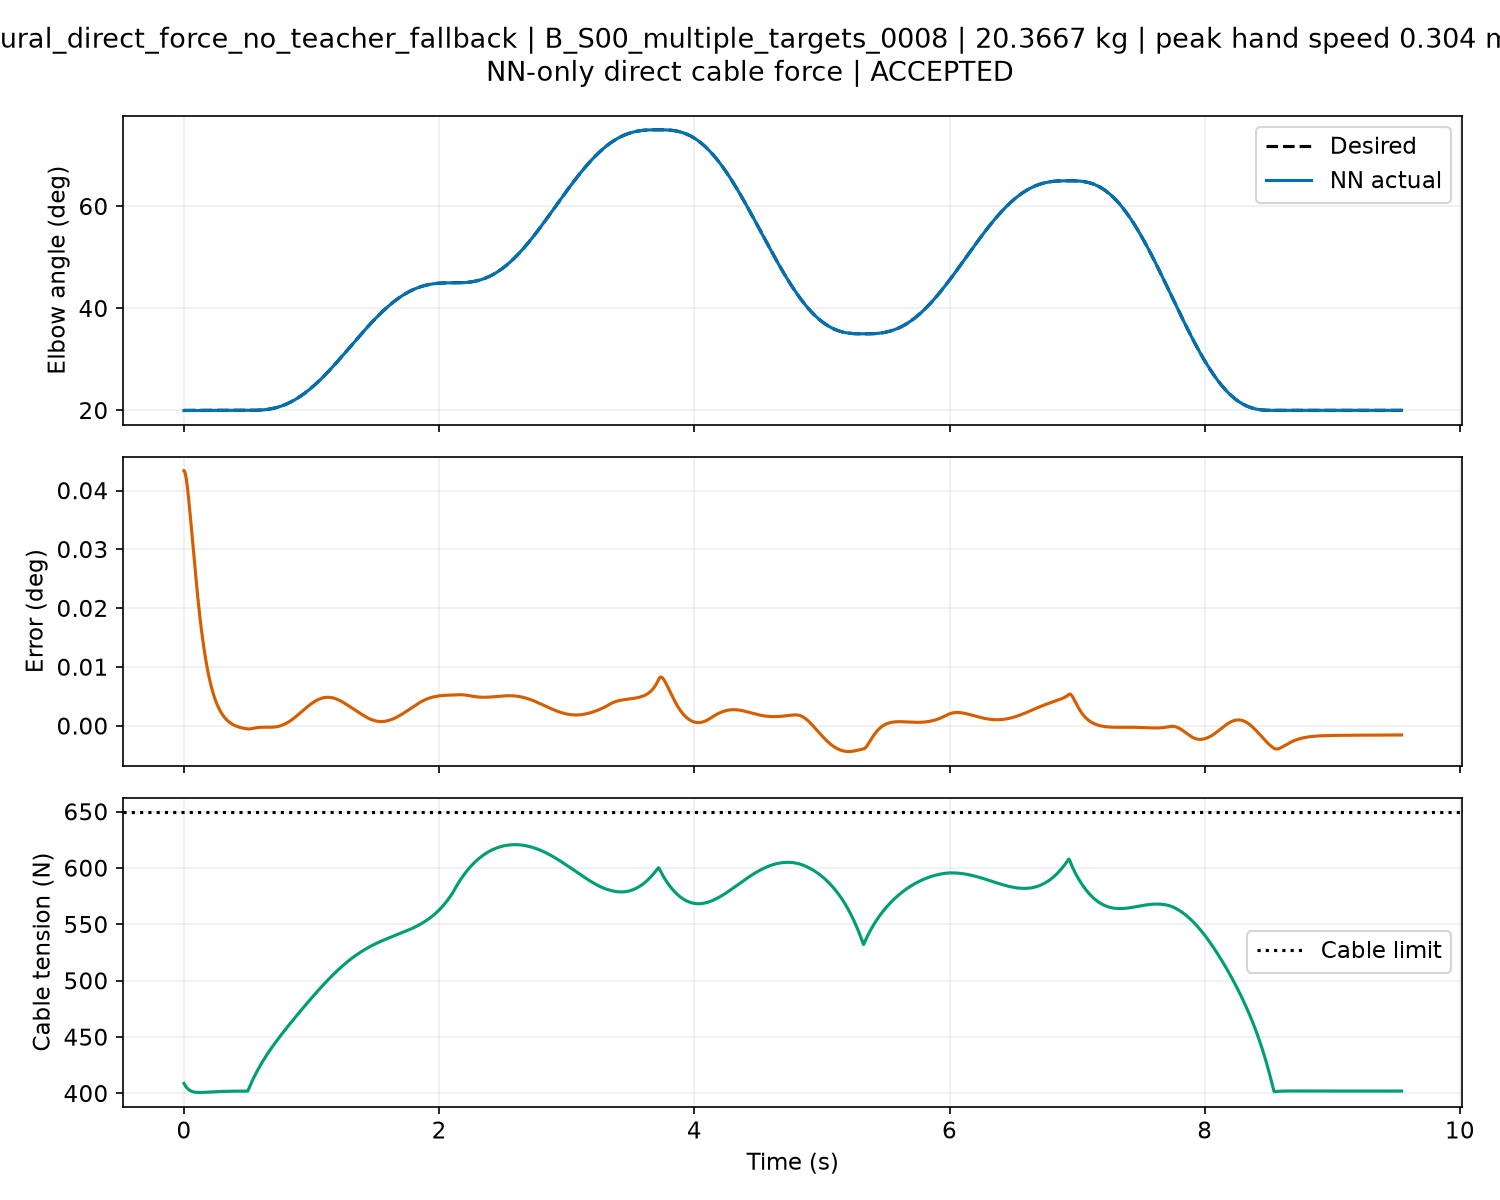
\includegraphics[width=\linewidth,height=0.69\textheight,keepaspectratio]{overleaf_figures/tracking_B_S00_multiple_targets_0008_tracking.png}
\caption{tracking/B\_S00\_multiple\_targets\_0008/tracking.png: Saved simulation diagnostics. Quantities and units are identified on the axes; failed runs are retained.}
\label{fig:tracking_B_S00_multiple_targets_0008_tracking}
\end{figure}
\begin{figure}[H]\centering
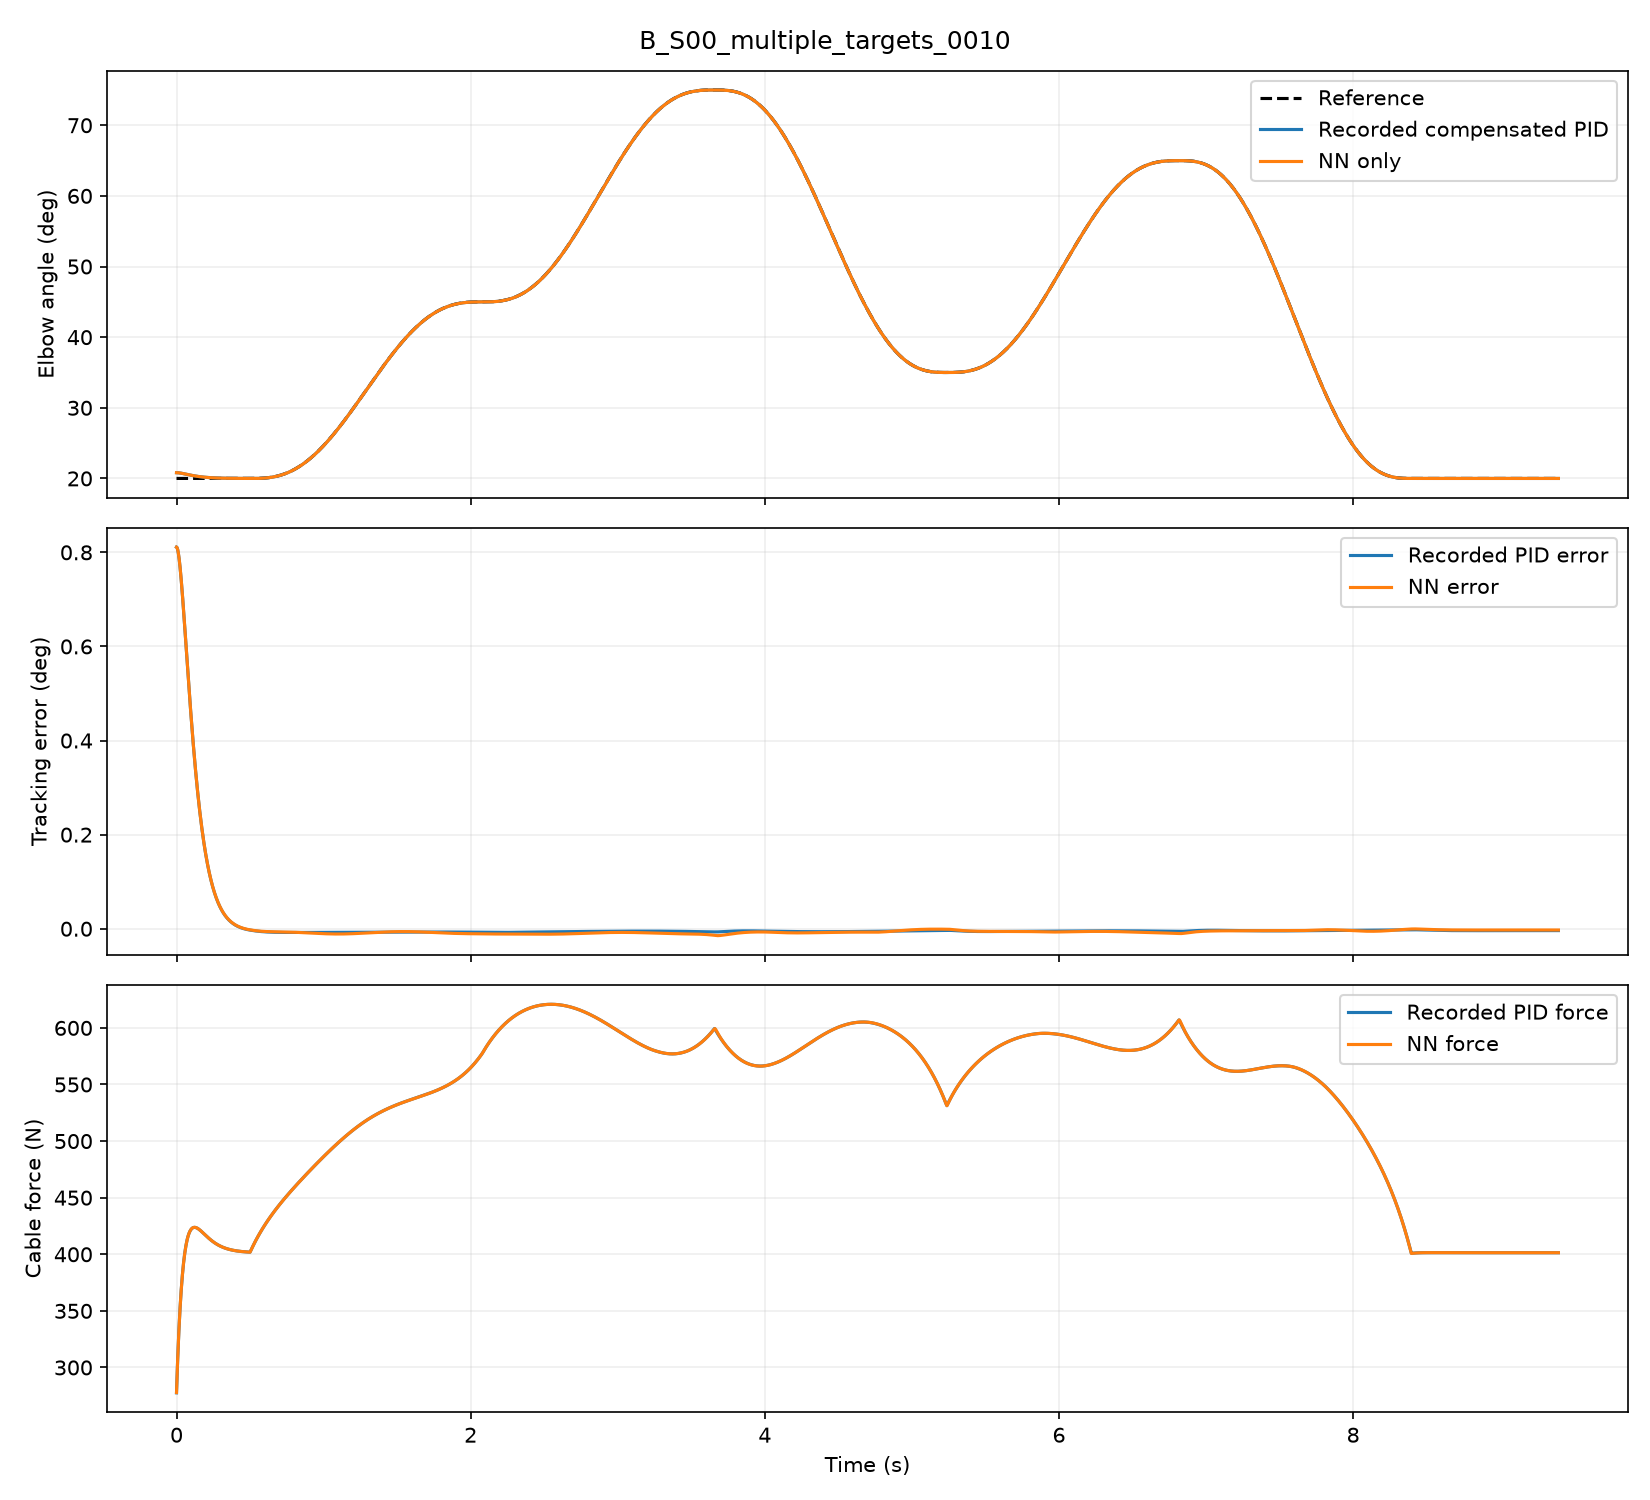
\includegraphics[width=\linewidth,height=0.69\textheight,keepaspectratio]{overleaf_figures/tracking_B_S00_multiple_targets_0010_comparison.png}
\caption{tracking/B\_S00\_multiple\_targets\_0010/comparison.png: Held-out OpenSim rollout: reference, recorded PID, and NN elbow motion; tracking errors; and cable forces. The NN supplies the cable command without a PID fallback.}
\label{fig:tracking_B_S00_multiple_targets_0010_comparison}
\end{figure}
\begin{figure}[H]\centering
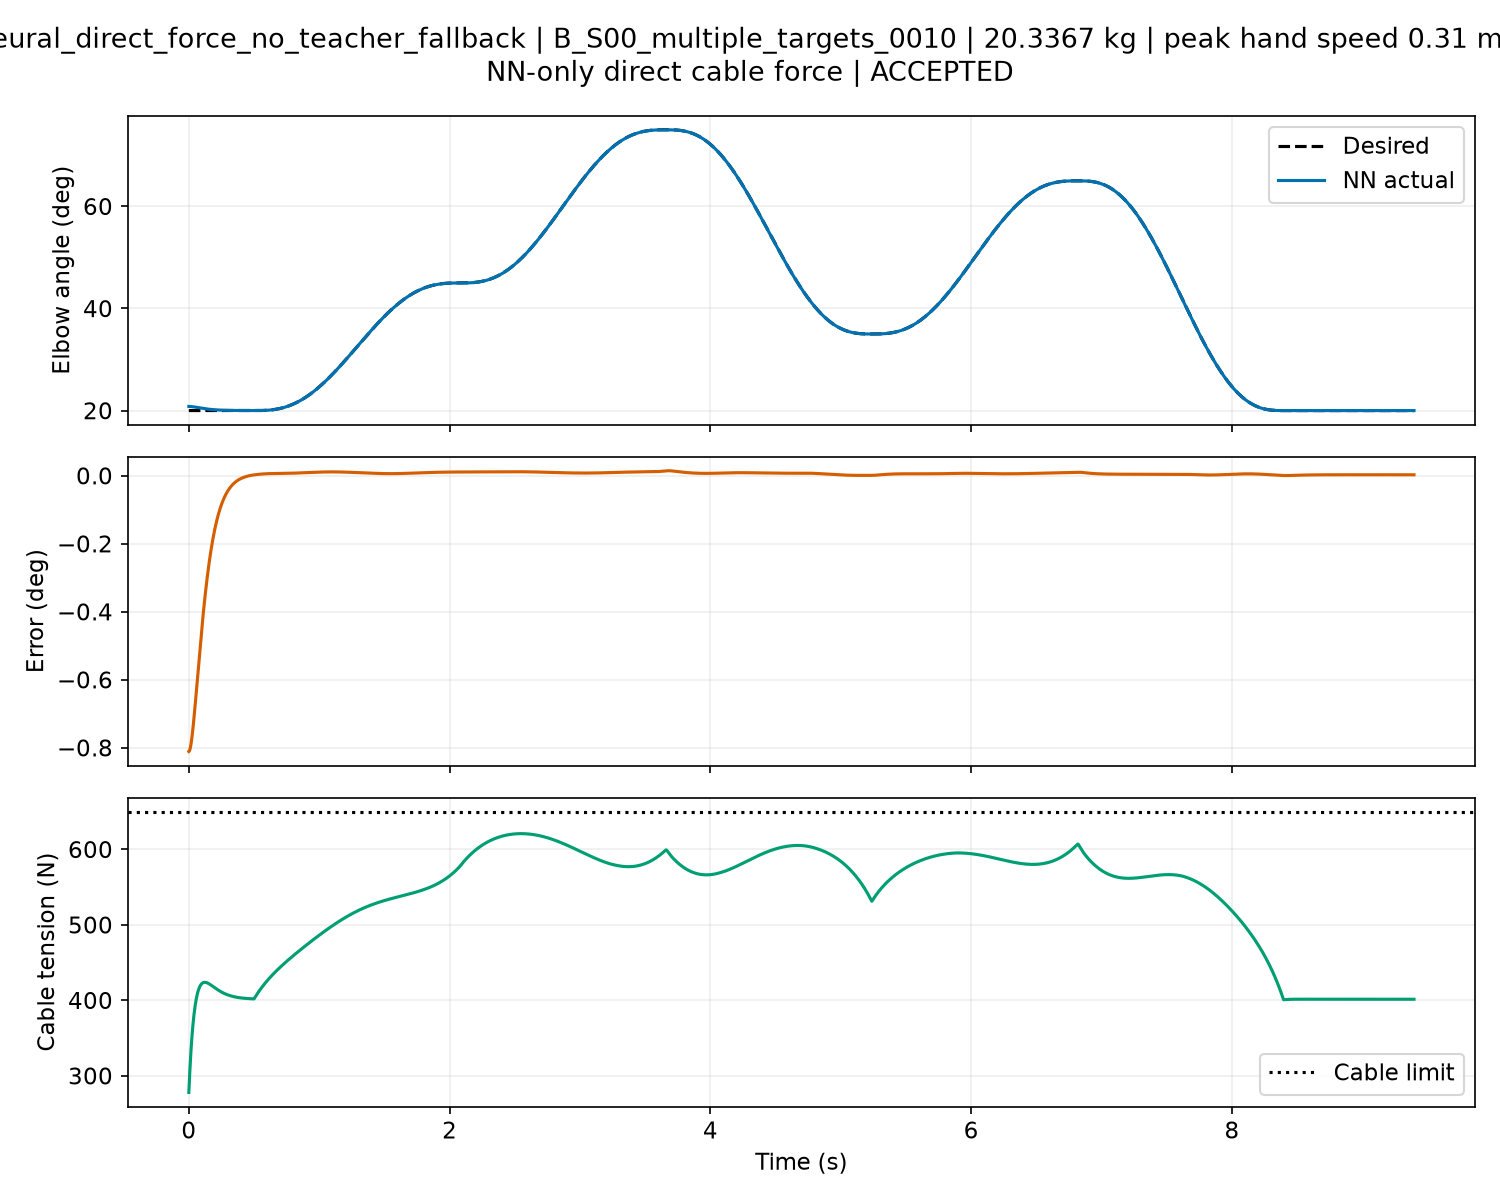
\includegraphics[width=\linewidth,height=0.69\textheight,keepaspectratio]{overleaf_figures/tracking_B_S00_multiple_targets_0010_tracking.png}
\caption{tracking/B\_S00\_multiple\_targets\_0010/tracking.png: Saved simulation diagnostics. Quantities and units are identified on the axes; failed runs are retained.}
\label{fig:tracking_B_S00_multiple_targets_0010_tracking}
\end{figure}
\begin{figure}[H]\centering
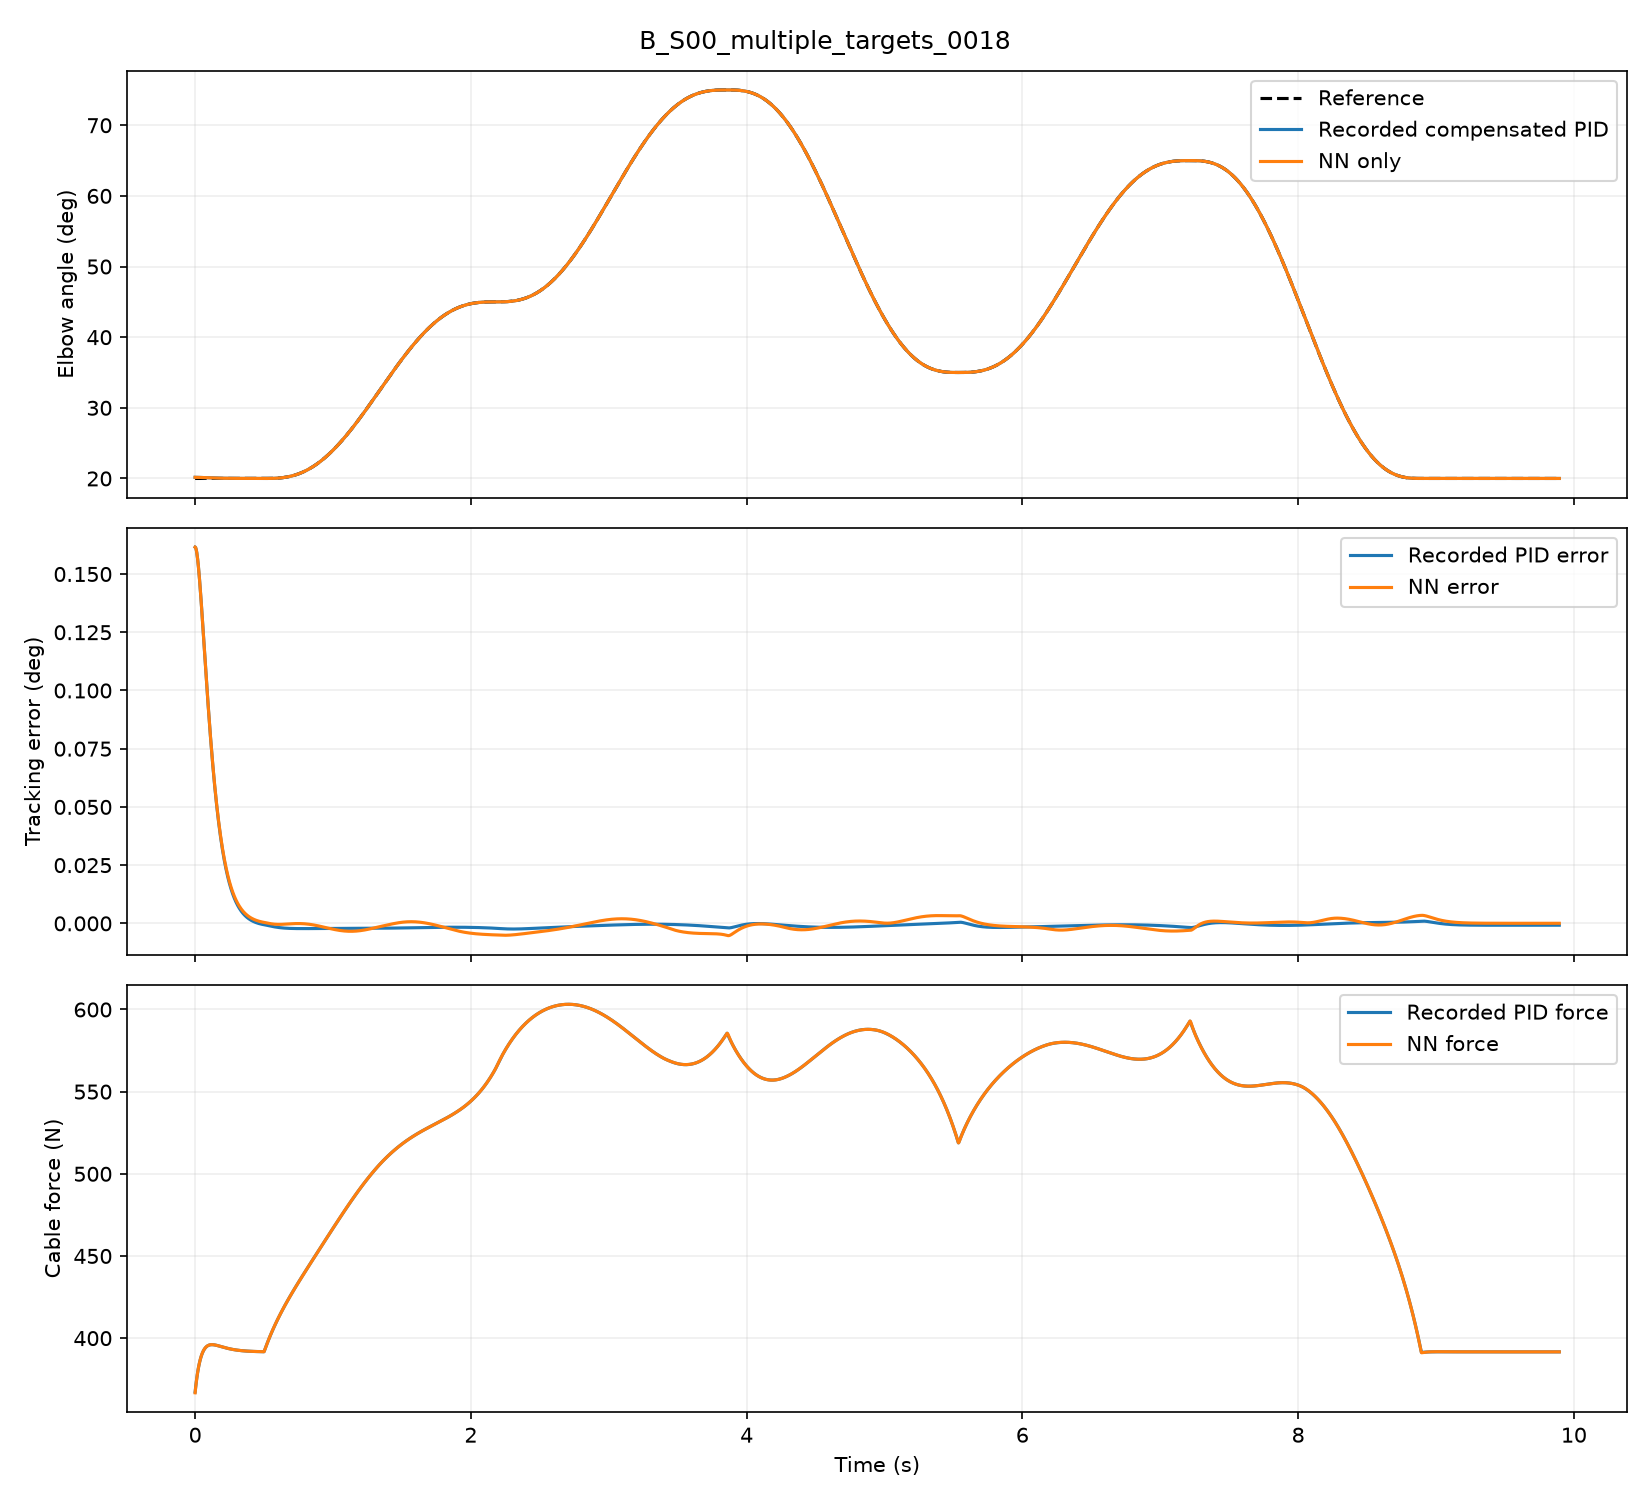
\includegraphics[width=\linewidth,height=0.69\textheight,keepaspectratio]{overleaf_figures/tracking_B_S00_multiple_targets_0018_comparison.png}
\caption{tracking/B\_S00\_multiple\_targets\_0018/comparison.png: Held-out OpenSim rollout: reference, recorded PID, and NN elbow motion; tracking errors; and cable forces. The NN supplies the cable command without a PID fallback.}
\label{fig:tracking_B_S00_multiple_targets_0018_comparison}
\end{figure}
\begin{figure}[H]\centering
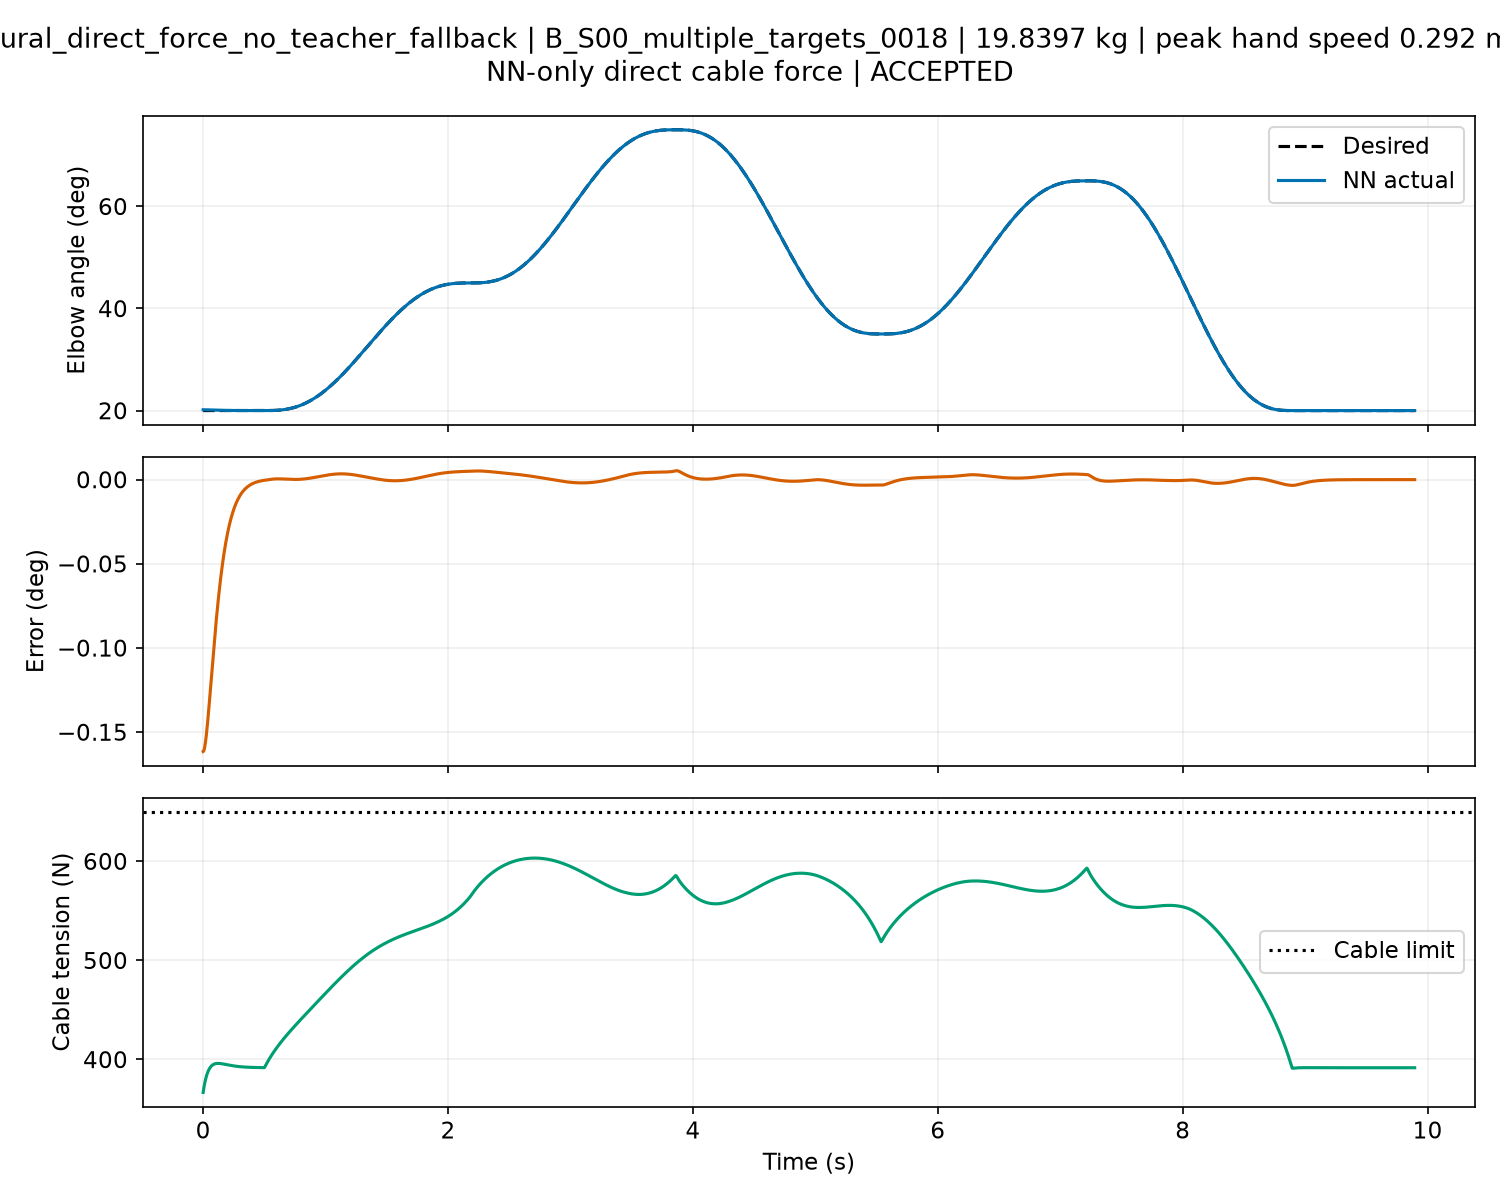
\includegraphics[width=\linewidth,height=0.69\textheight,keepaspectratio]{overleaf_figures/tracking_B_S00_multiple_targets_0018_tracking.png}
\caption{tracking/B\_S00\_multiple\_targets\_0018/tracking.png: Saved simulation diagnostics. Quantities and units are identified on the axes; failed runs are retained.}
\label{fig:tracking_B_S00_multiple_targets_0018_tracking}
\end{figure}
\begin{figure}[H]\centering
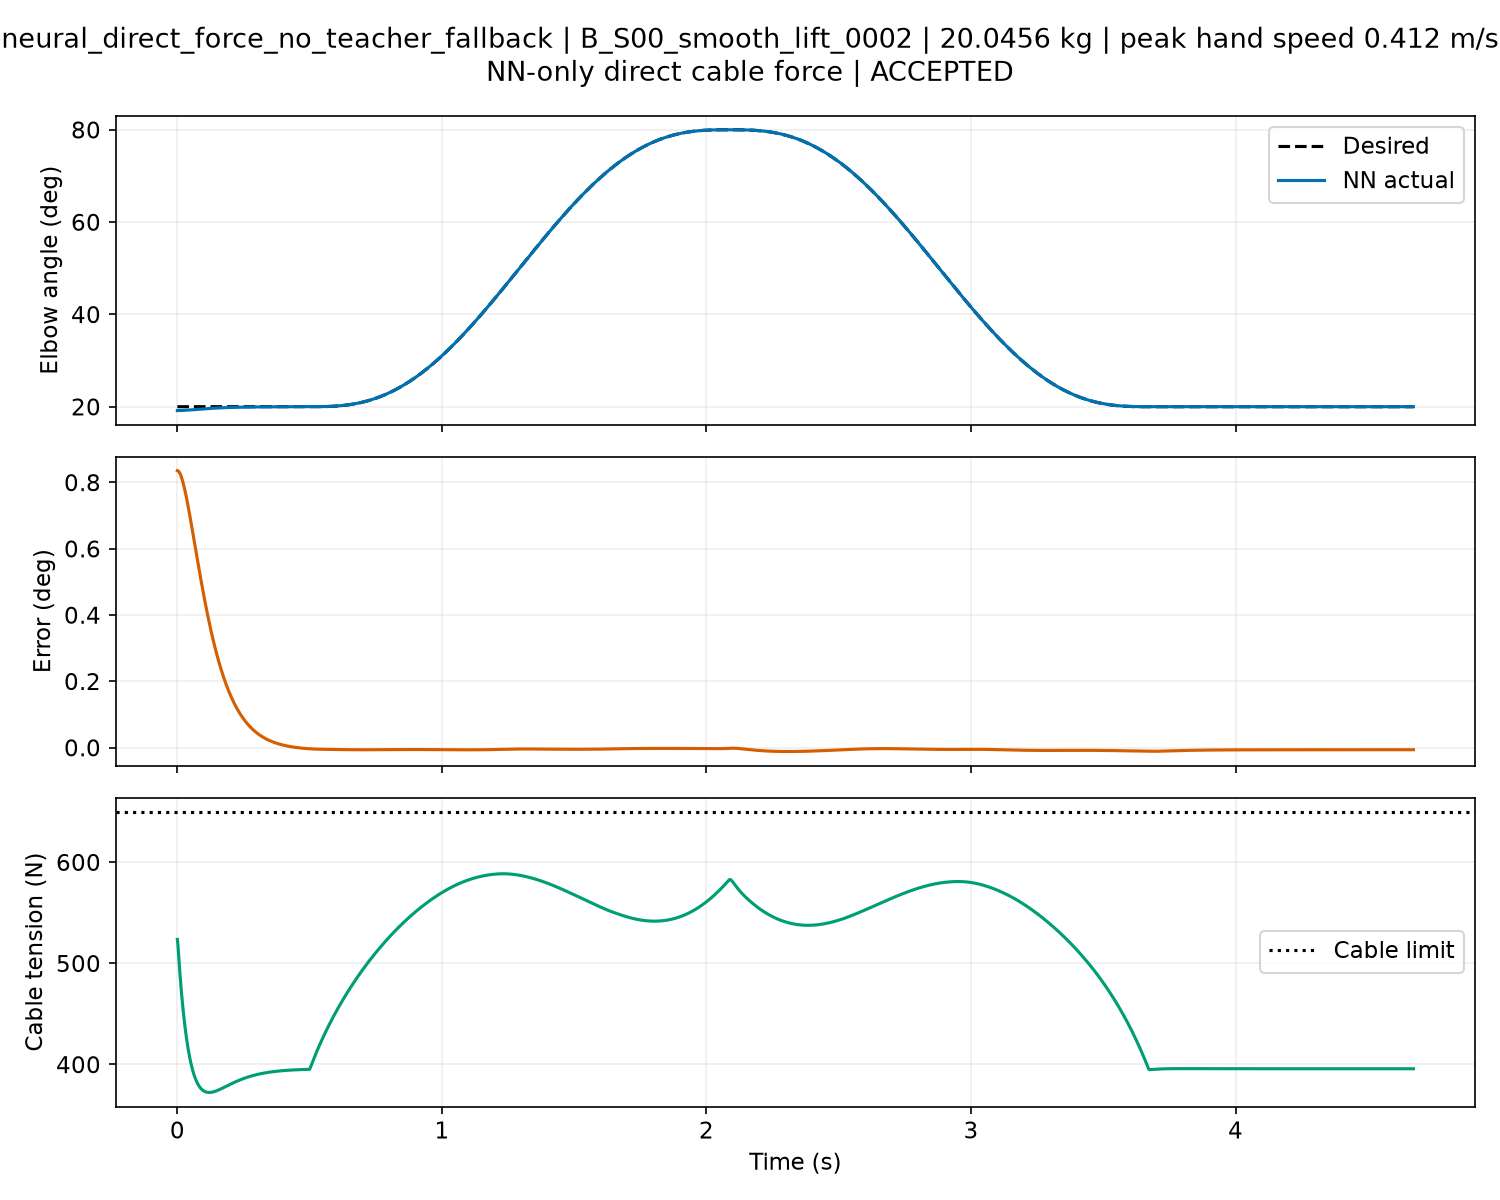
\includegraphics[width=\linewidth,height=0.69\textheight,keepaspectratio]{overleaf_figures/tracking_B_S00_smooth_lift_0002_tracking.png}
\caption{tracking/B\_S00\_smooth\_lift\_0002/tracking.png: Saved simulation diagnostics. Quantities and units are identified on the axes; failed runs are retained.}
\label{fig:tracking_B_S00_smooth_lift_0002_tracking}
\end{figure}
\begin{figure}[H]\centering
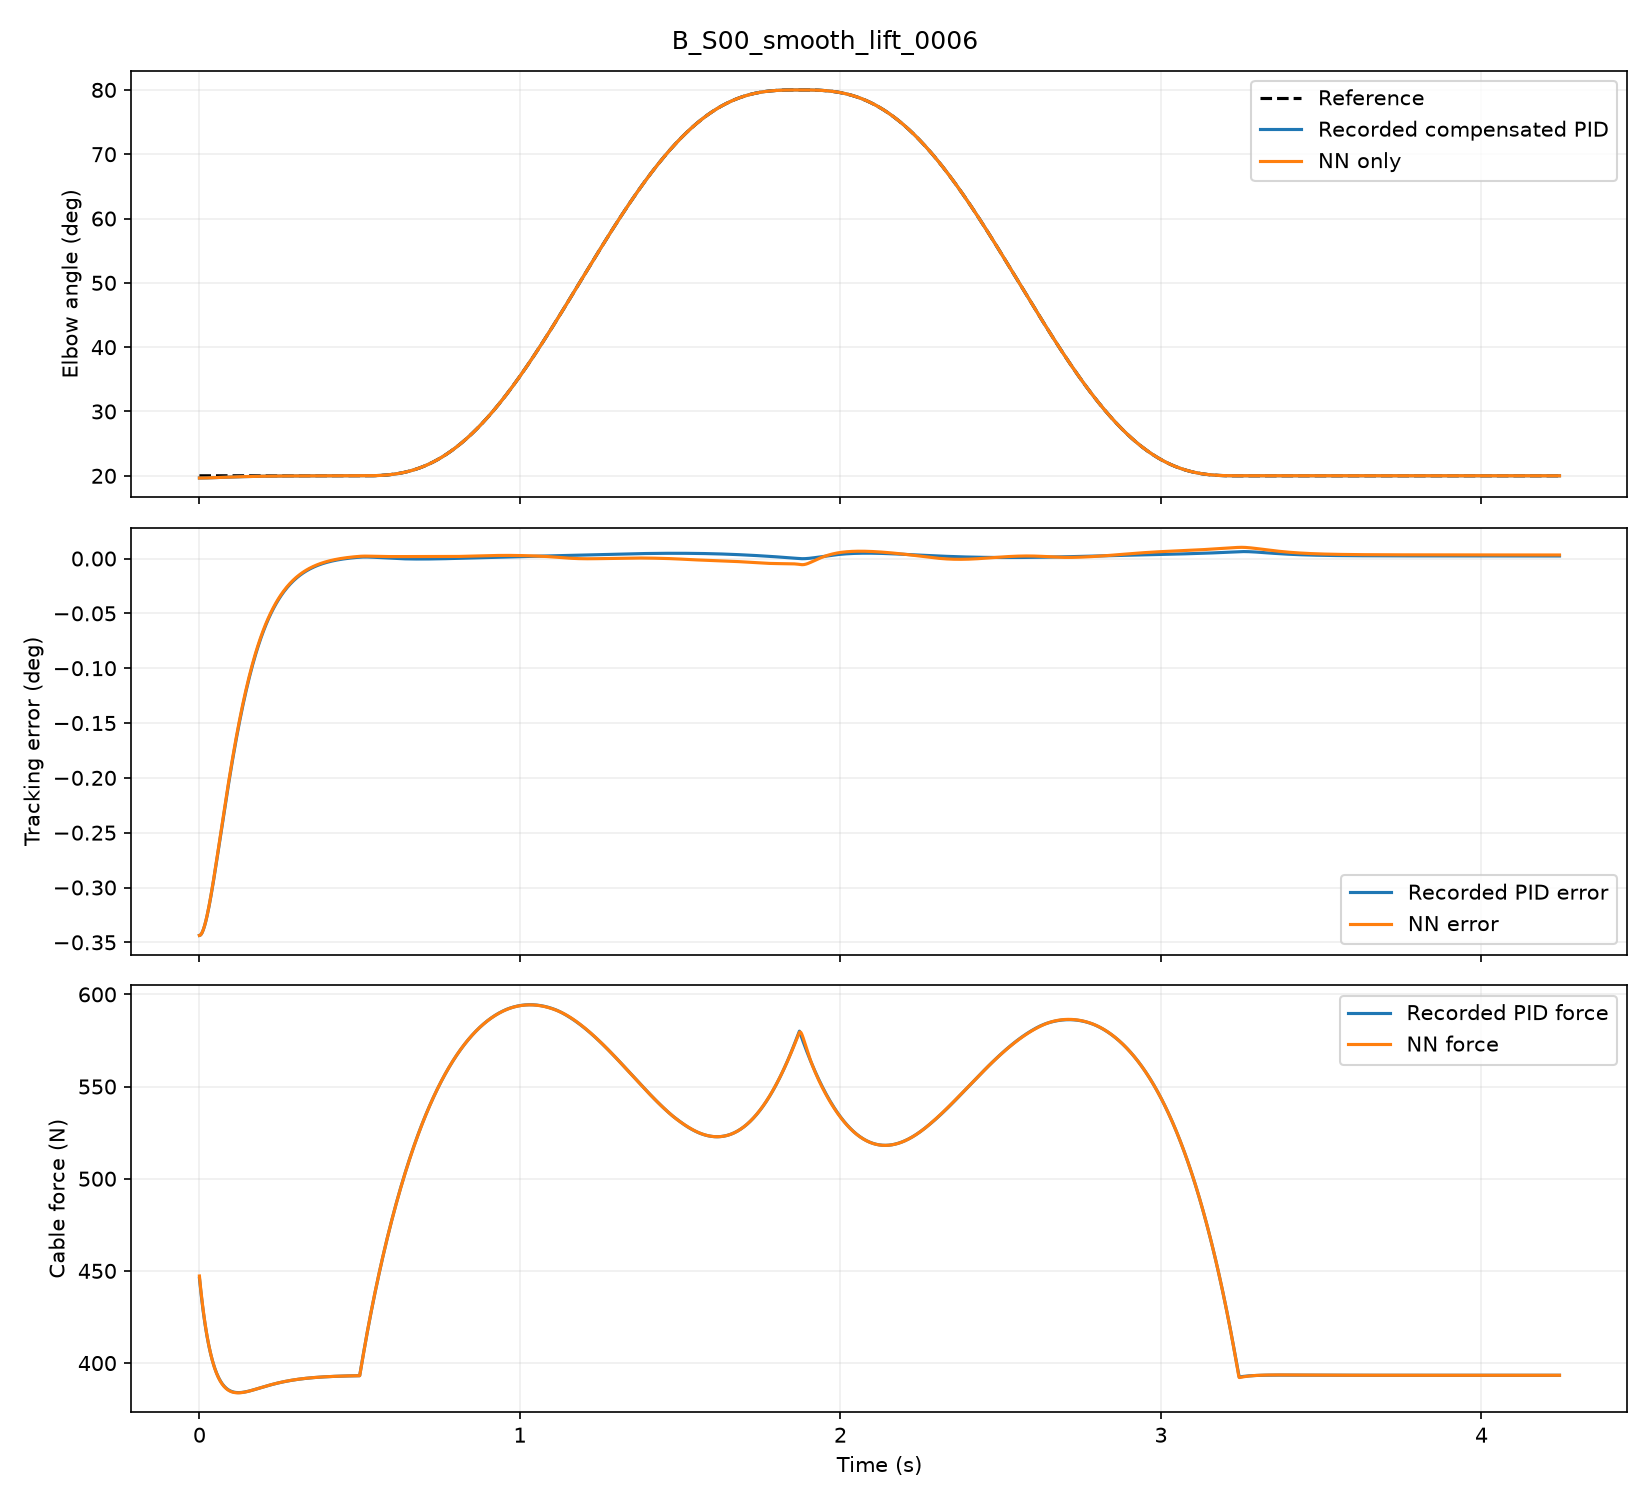
\includegraphics[width=\linewidth,height=0.69\textheight,keepaspectratio]{overleaf_figures/tracking_B_S00_smooth_lift_0006_comparison.png}
\caption{tracking/B\_S00\_smooth\_lift\_0006/comparison.png: Held-out OpenSim rollout: reference, recorded PID, and NN elbow motion; tracking errors; and cable forces. The NN supplies the cable command without a PID fallback.}
\label{fig:tracking_B_S00_smooth_lift_0006_comparison}
\end{figure}
\begin{figure}[H]\centering
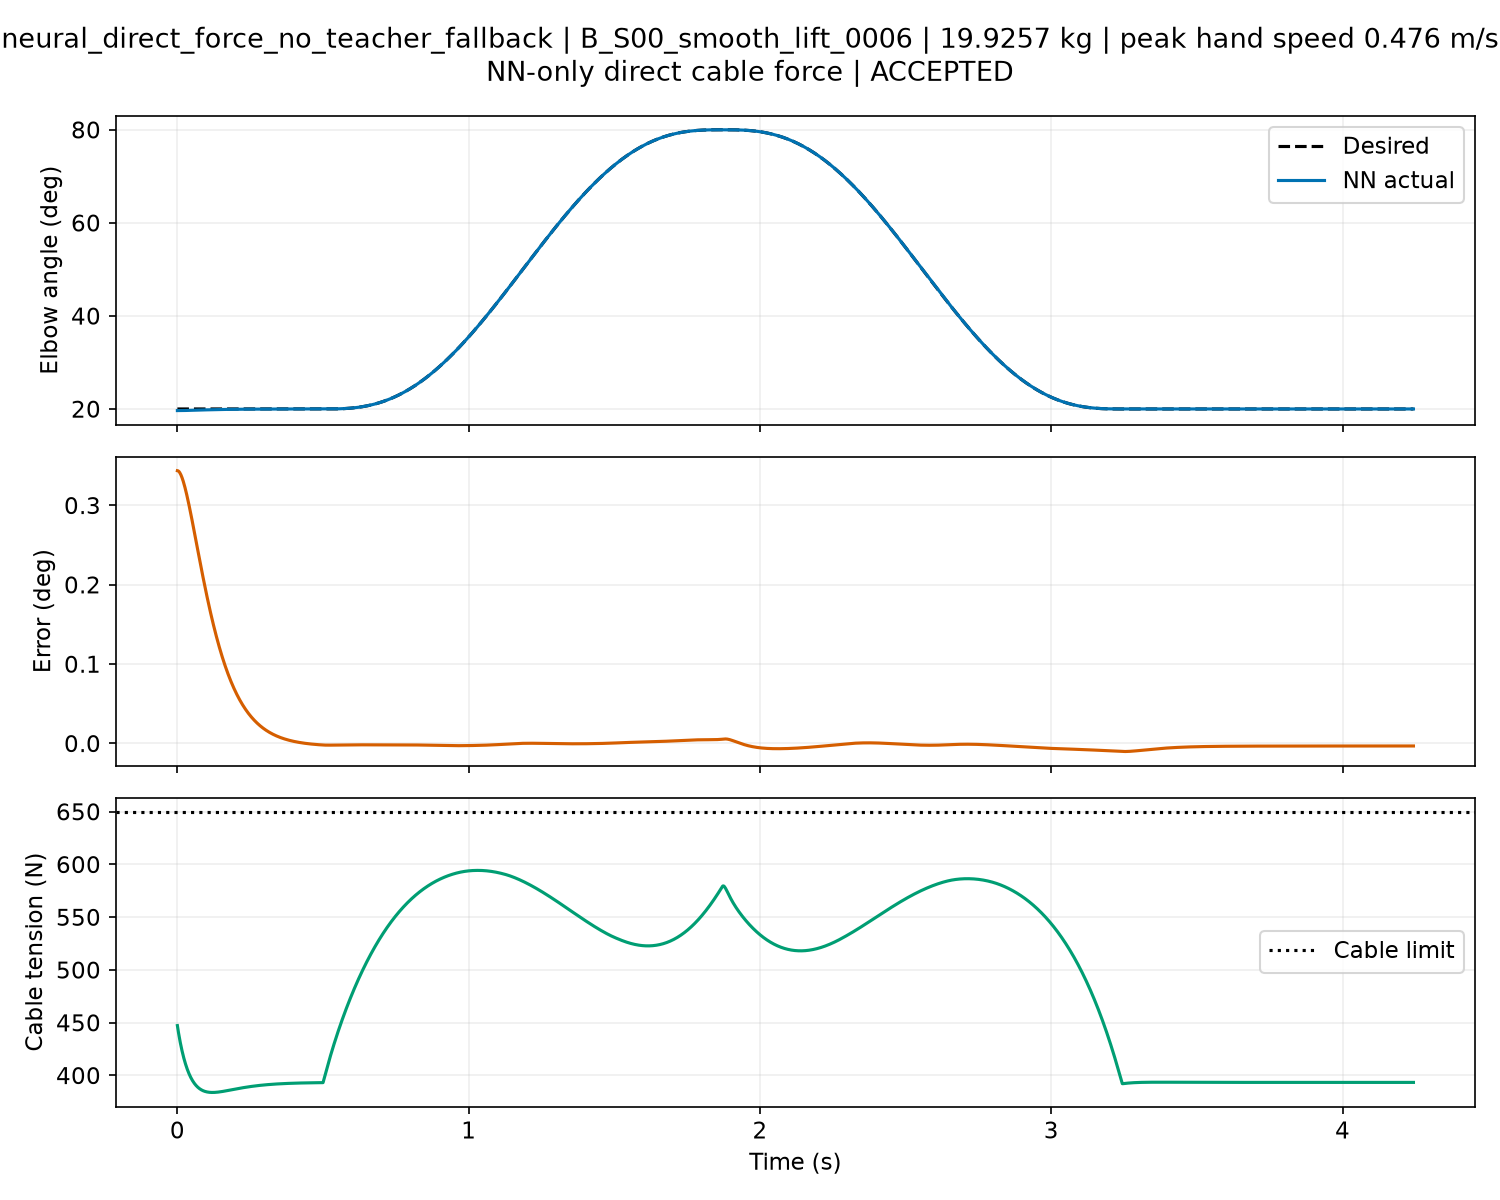
\includegraphics[width=\linewidth,height=0.69\textheight,keepaspectratio]{overleaf_figures/tracking_B_S00_smooth_lift_0006_tracking.png}
\caption{tracking/B\_S00\_smooth\_lift\_0006/tracking.png: Saved simulation diagnostics. Quantities and units are identified on the axes; failed runs are retained.}
\label{fig:tracking_B_S00_smooth_lift_0006_tracking}
\end{figure}
\begin{figure}[H]\centering
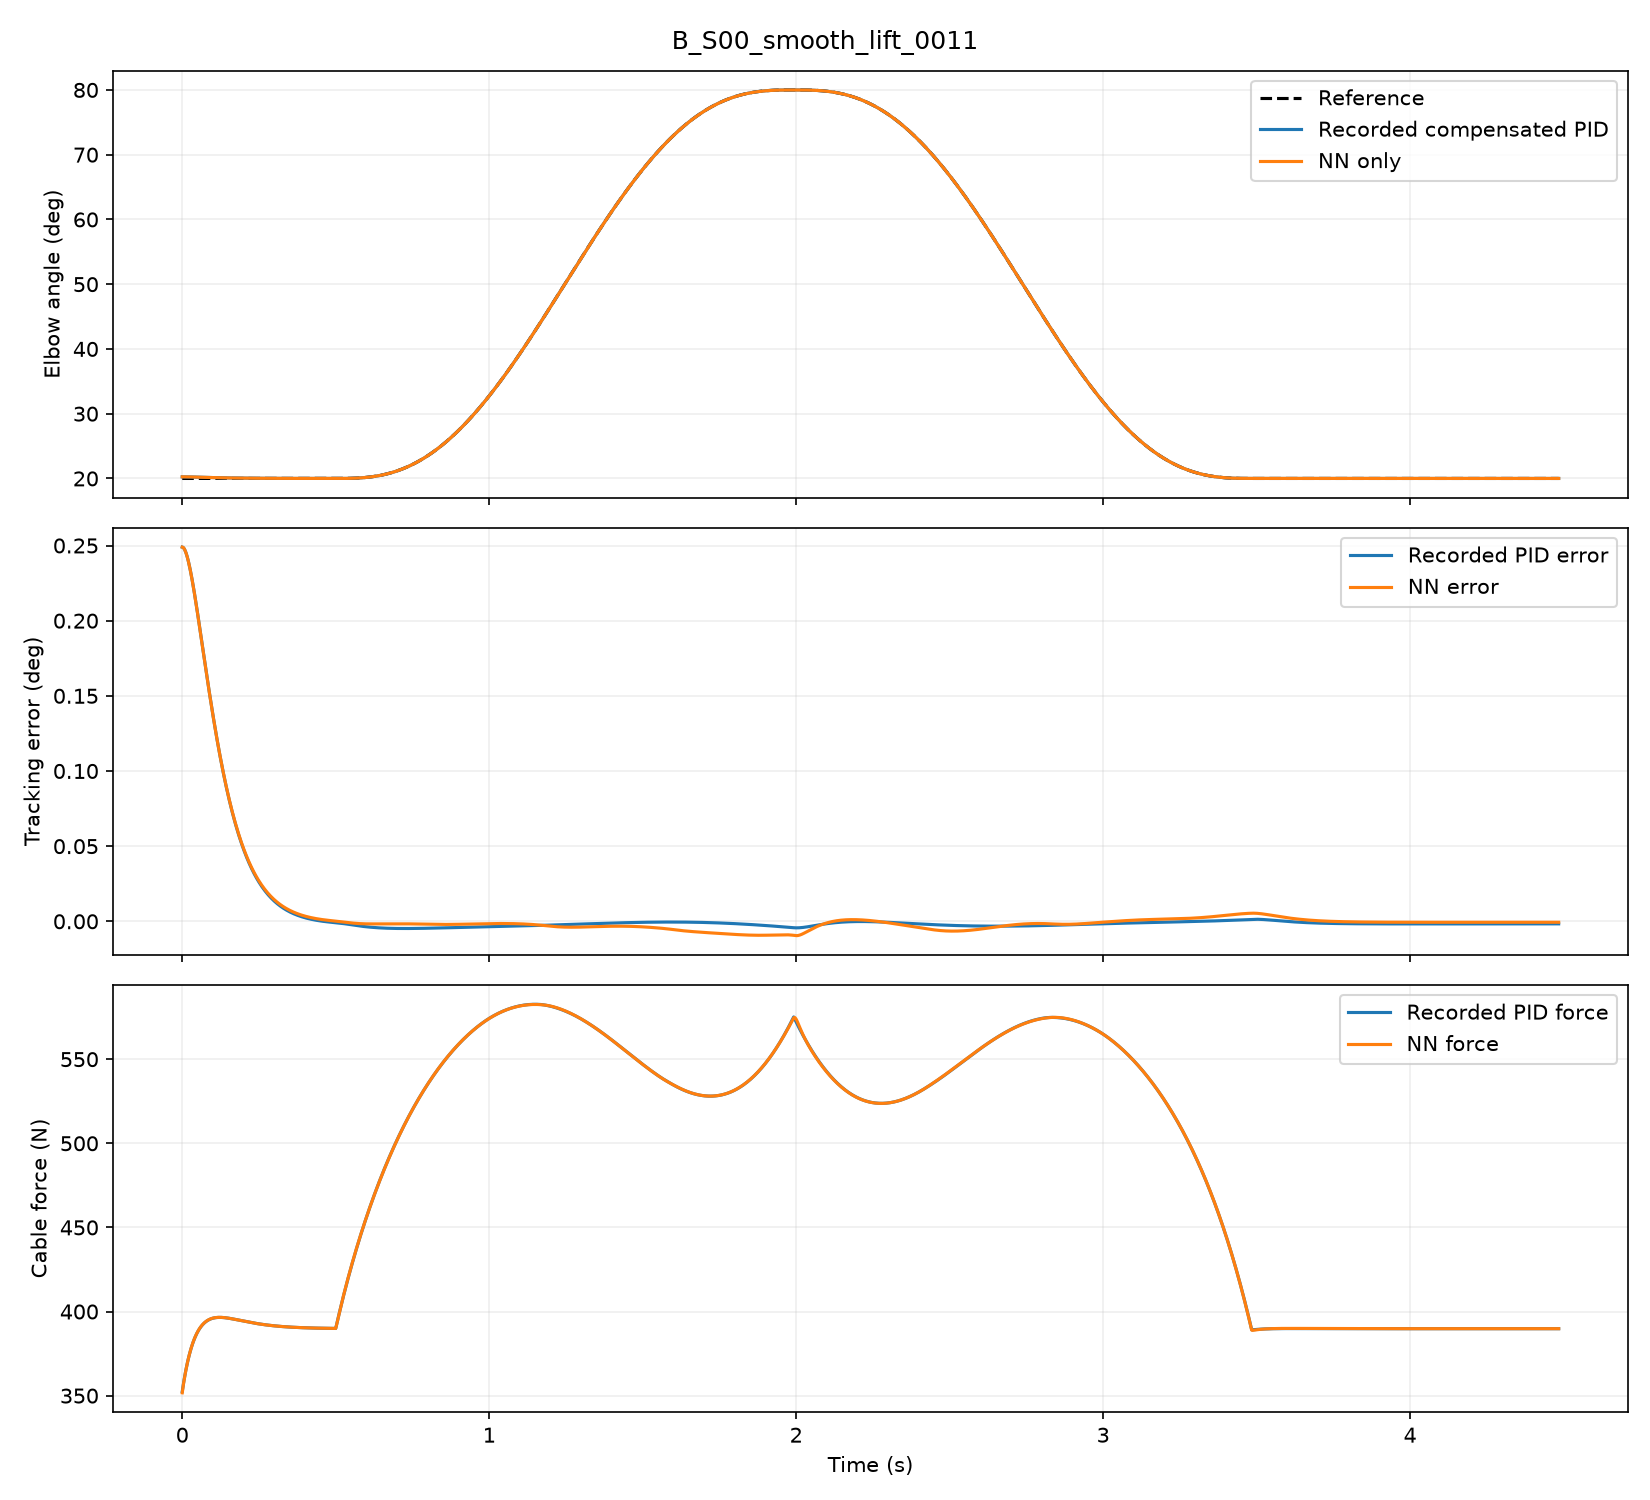
\includegraphics[width=\linewidth,height=0.69\textheight,keepaspectratio]{overleaf_figures/tracking_B_S00_smooth_lift_0011_comparison.png}
\caption{tracking/B\_S00\_smooth\_lift\_0011/comparison.png: Held-out OpenSim rollout: reference, recorded PID, and NN elbow motion; tracking errors; and cable forces. The NN supplies the cable command without a PID fallback.}
\label{fig:tracking_B_S00_smooth_lift_0011_comparison}
\end{figure}
\begin{figure}[H]\centering
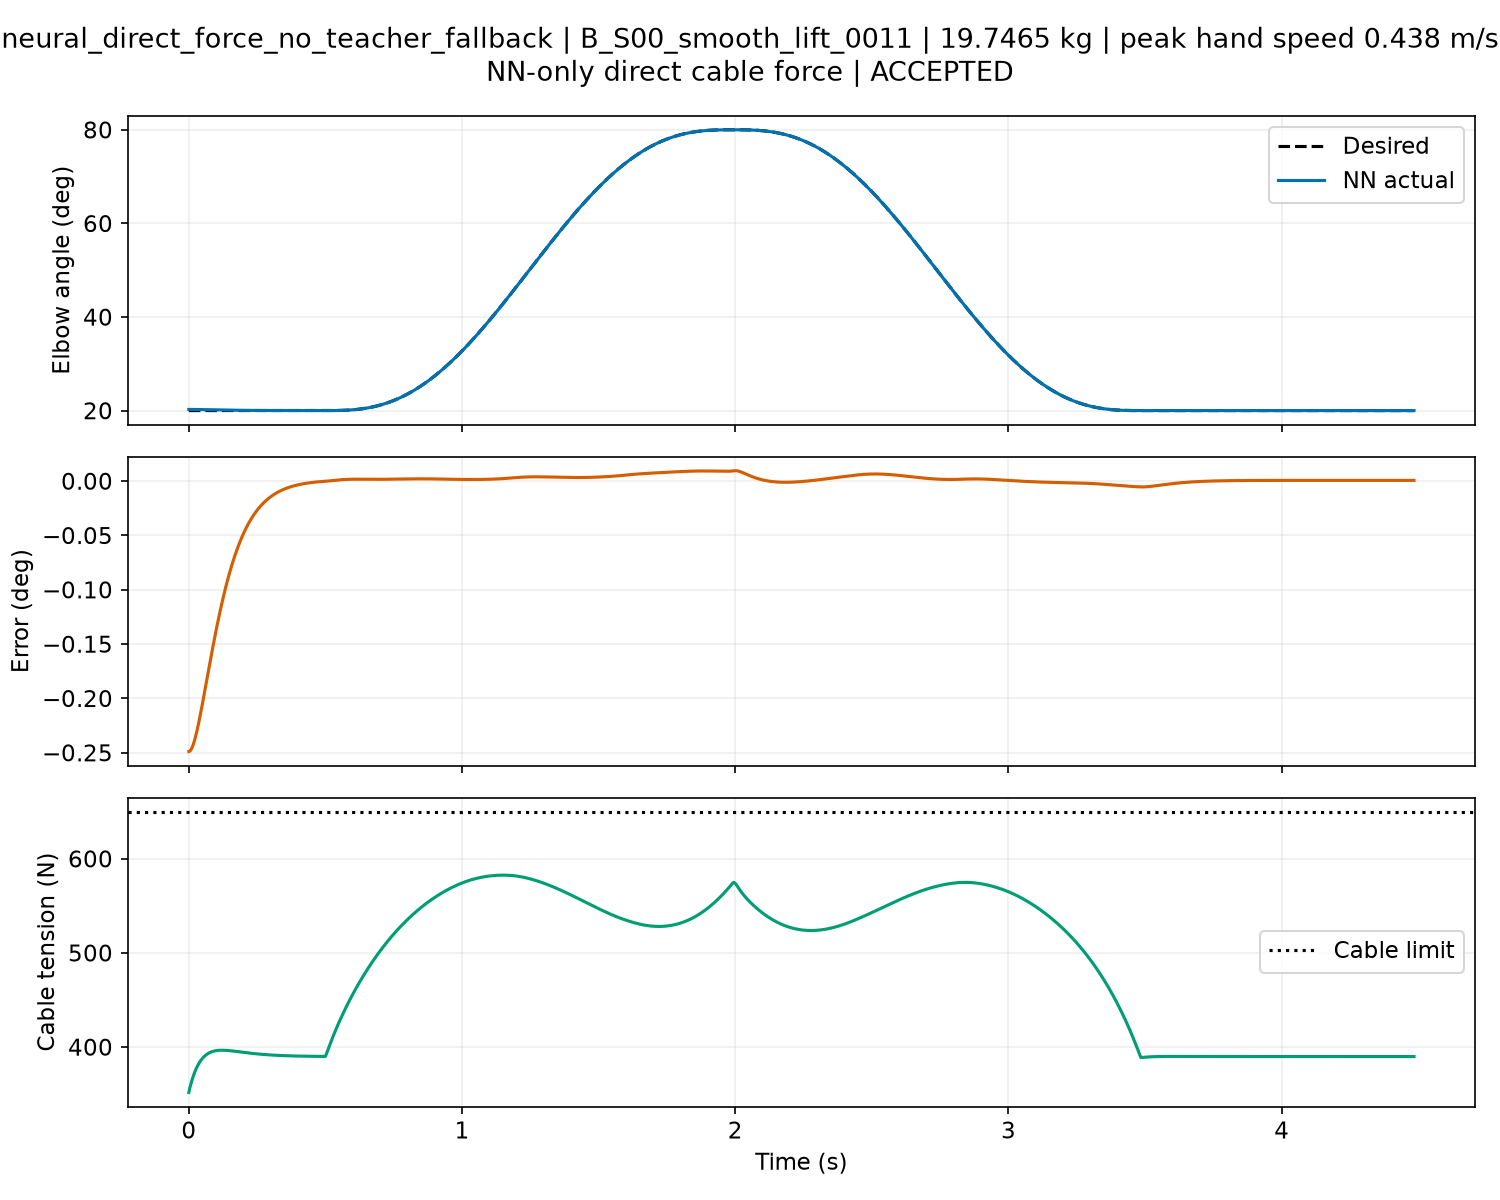
\includegraphics[width=\linewidth,height=0.69\textheight,keepaspectratio]{overleaf_figures/tracking_B_S00_smooth_lift_0011_tracking.png}
\caption{tracking/B\_S00\_smooth\_lift\_0011/tracking.png: Saved simulation diagnostics. Quantities and units are identified on the axes; failed runs are retained.}
\label{fig:tracking_B_S00_smooth_lift_0011_tracking}
\end{figure}
\begin{figure}[H]\centering
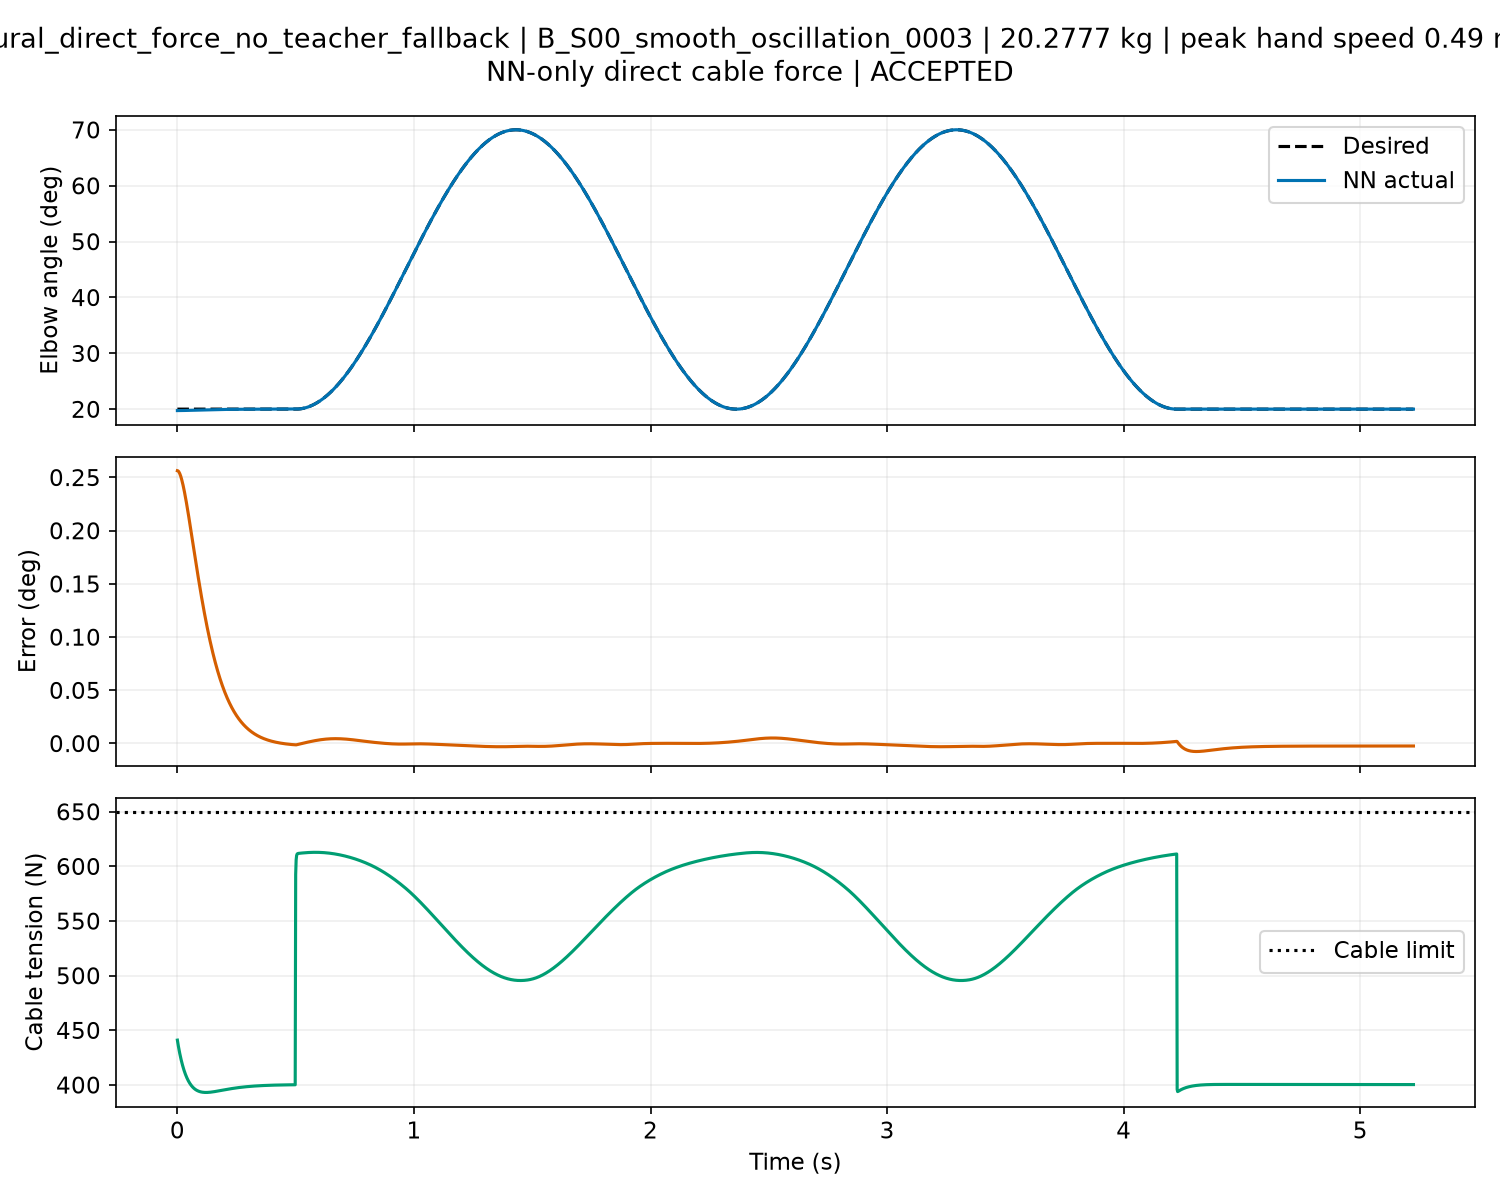
\includegraphics[width=\linewidth,height=0.69\textheight,keepaspectratio]{overleaf_figures/tracking_B_S00_smooth_oscillation_0003_tracking.png}
\caption{tracking/B\_S00\_smooth\_oscillation\_0003/tracking.png: Saved simulation diagnostics. Quantities and units are identified on the axes; failed runs are retained.}
\label{fig:tracking_B_S00_smooth_oscillation_0003_tracking}
\end{figure}
\begin{figure}[H]\centering
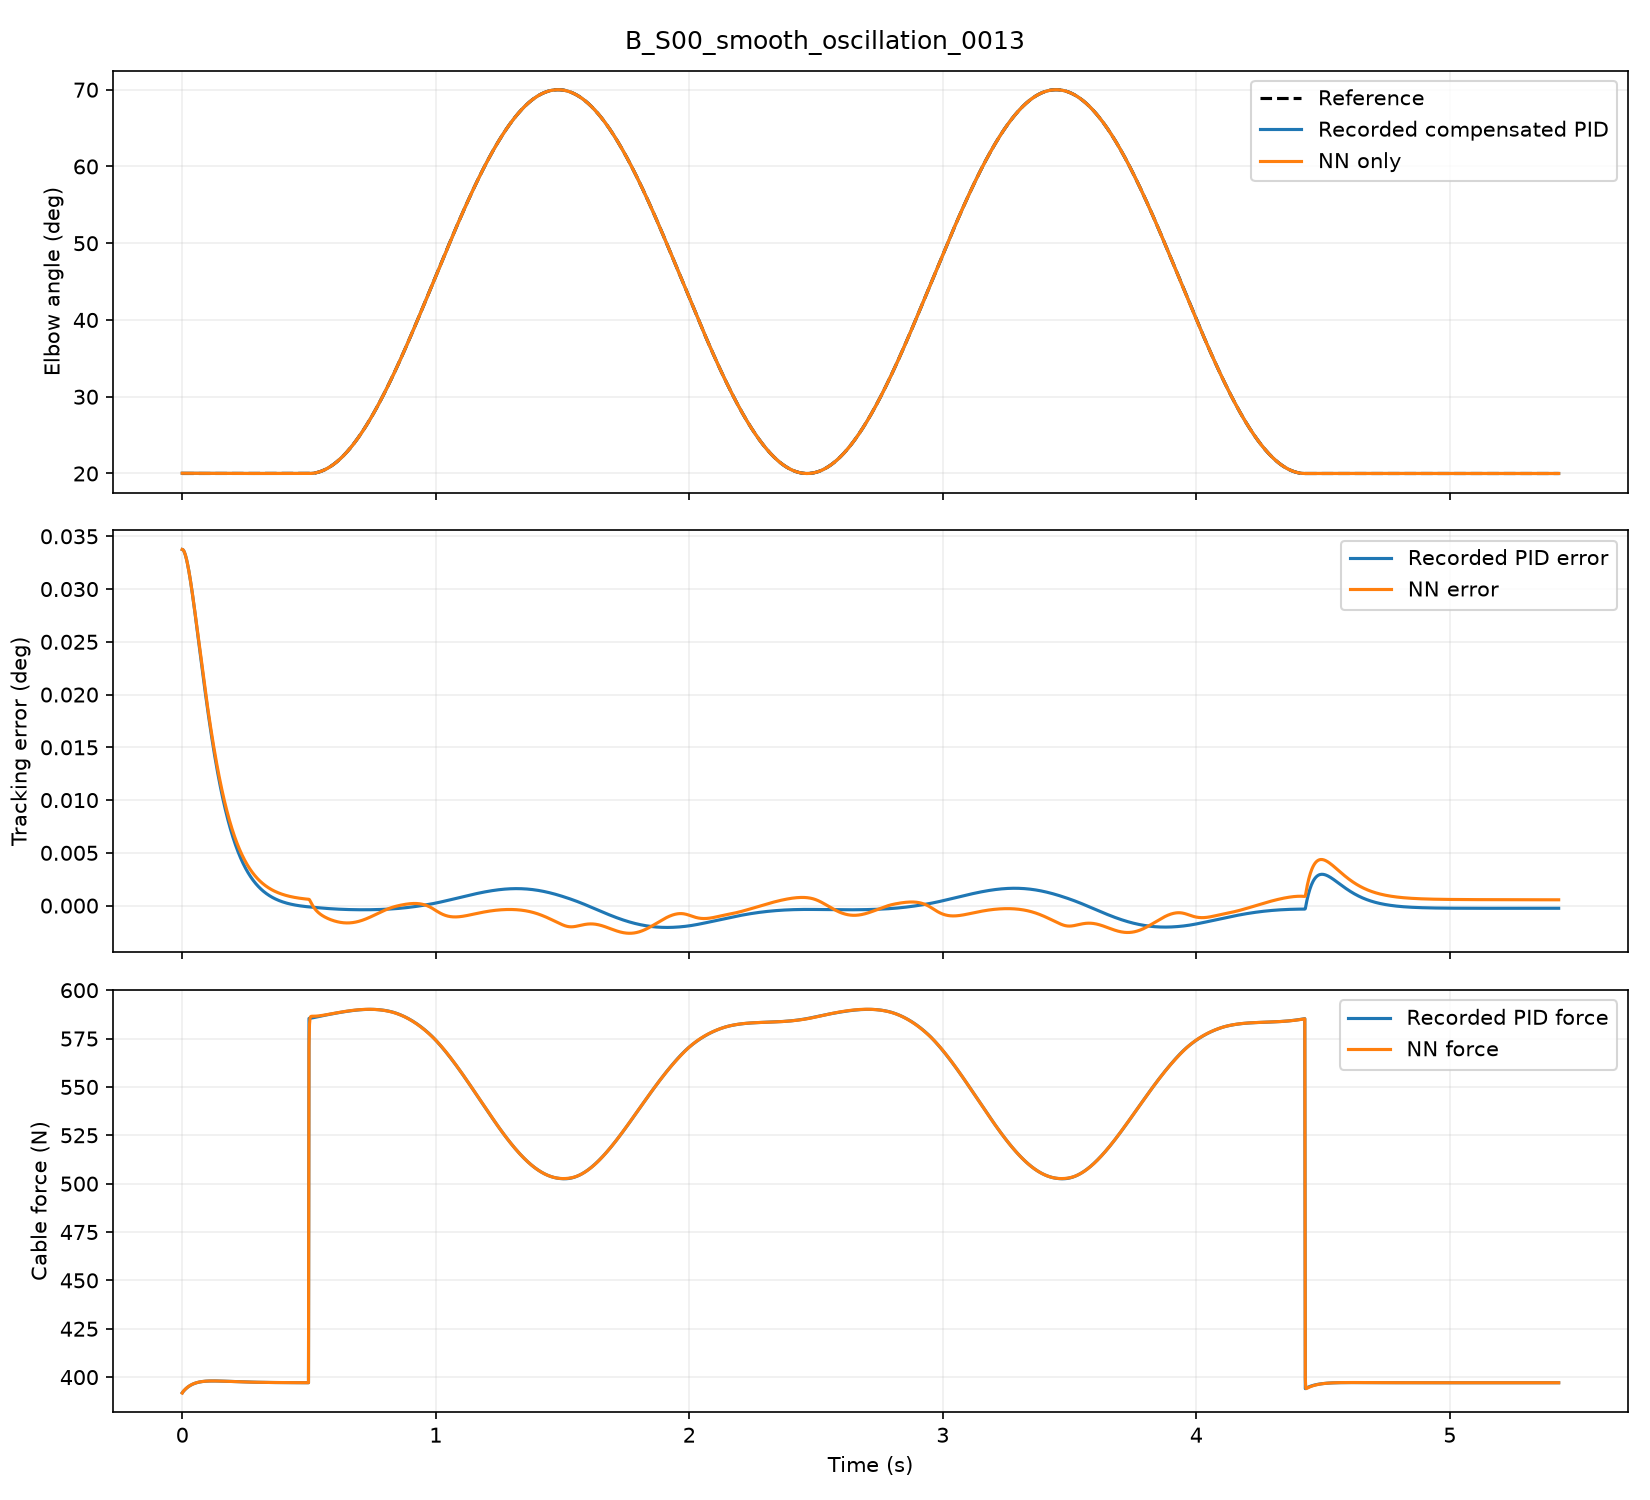
\includegraphics[width=\linewidth,height=0.69\textheight,keepaspectratio]{overleaf_figures/tracking_B_S00_smooth_oscillation_0013_comparison.png}
\caption{tracking/B\_S00\_smooth\_oscillation\_0013/comparison.png: Held-out OpenSim rollout: reference, recorded PID, and NN elbow motion; tracking errors; and cable forces. The NN supplies the cable command without a PID fallback.}
\label{fig:tracking_B_S00_smooth_oscillation_0013_comparison}
\end{figure}
\begin{figure}[H]\centering
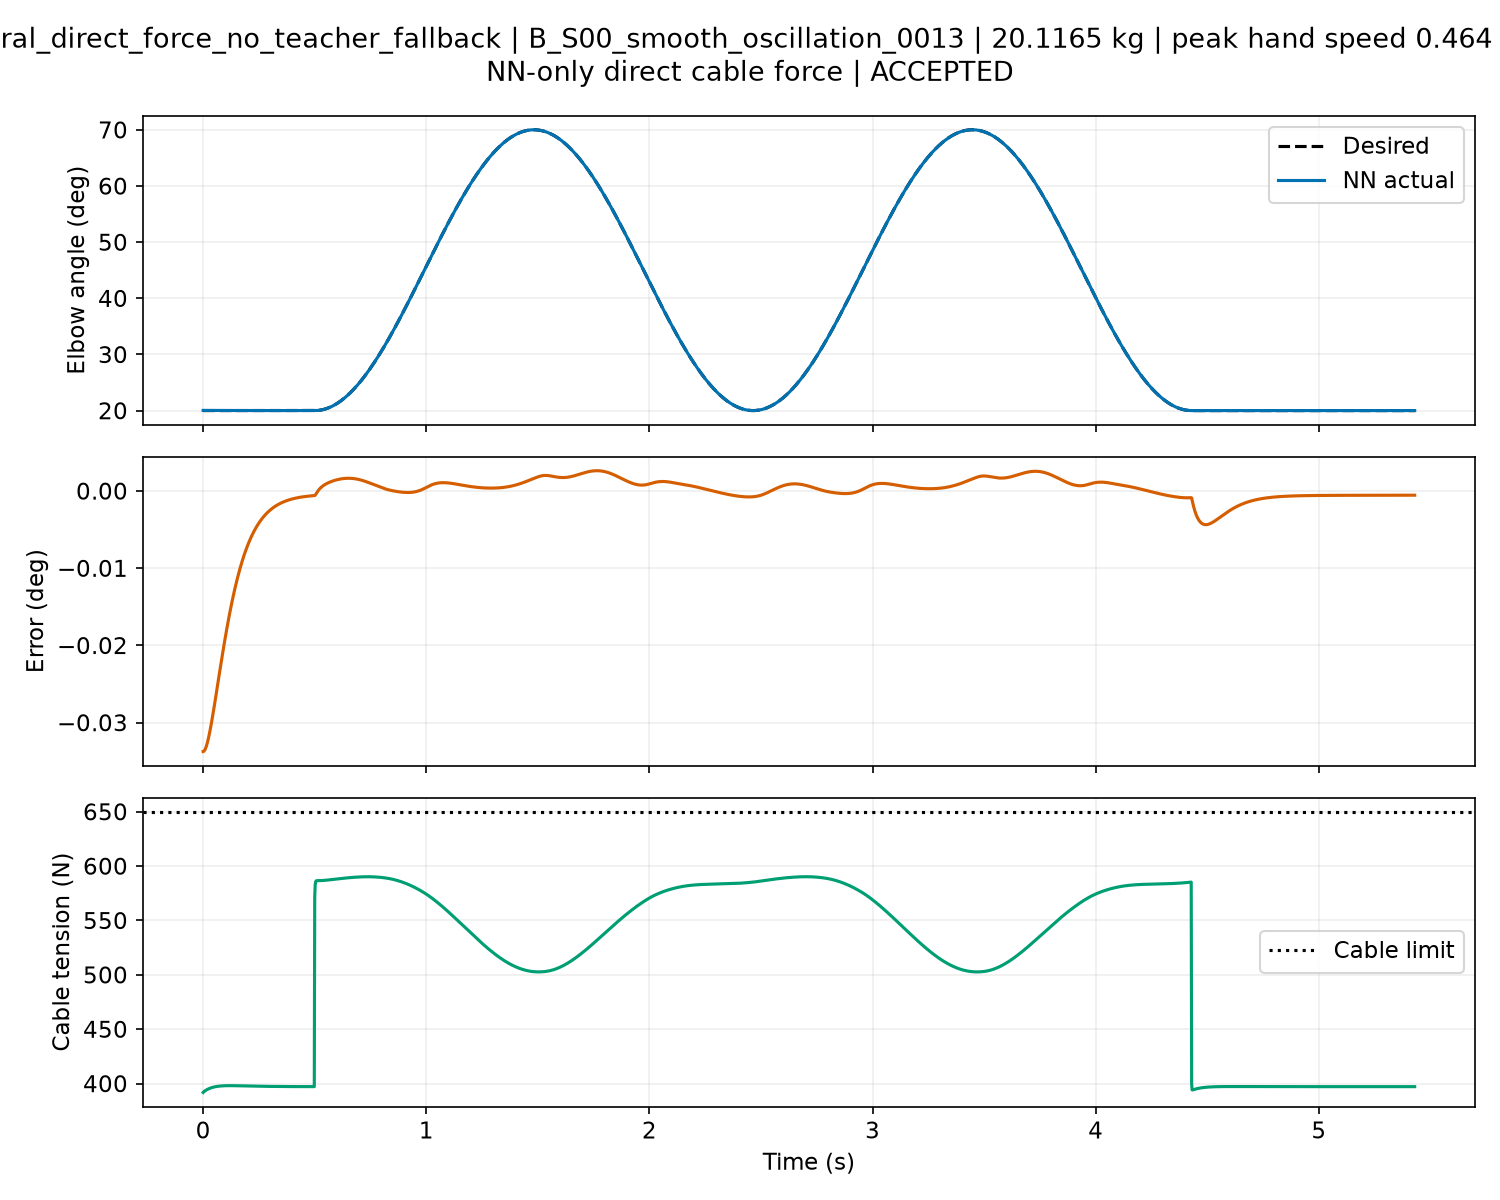
\includegraphics[width=\linewidth,height=0.69\textheight,keepaspectratio]{overleaf_figures/tracking_B_S00_smooth_oscillation_0013_tracking.png}
\caption{tracking/B\_S00\_smooth\_oscillation\_0013/tracking.png: Saved simulation diagnostics. Quantities and units are identified on the axes; failed runs are retained.}
\label{fig:tracking_B_S00_smooth_oscillation_0013_tracking}
\end{figure}
\begin{figure}[H]\centering
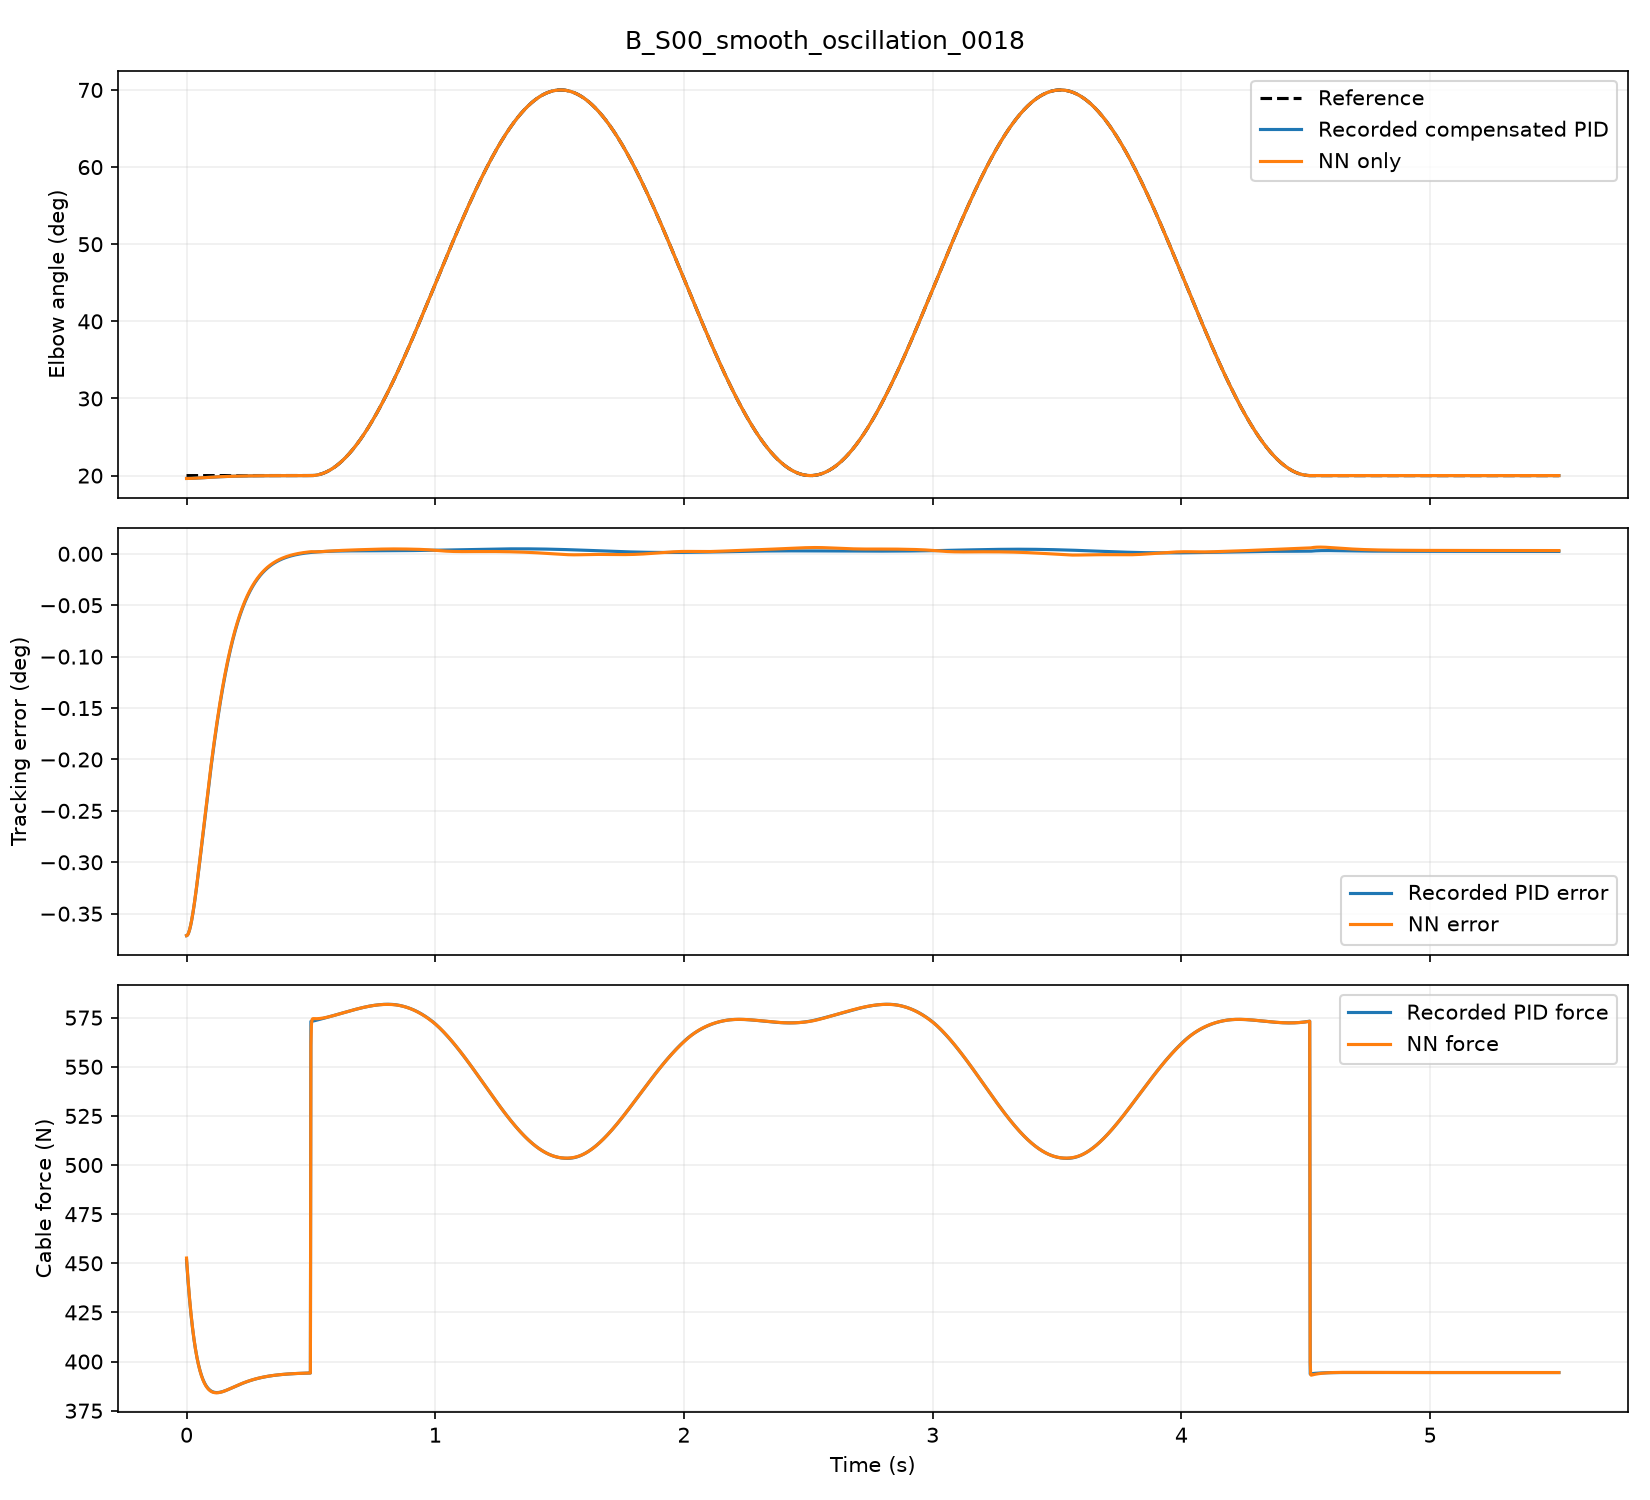
\includegraphics[width=\linewidth,height=0.69\textheight,keepaspectratio]{overleaf_figures/tracking_B_S00_smooth_oscillation_0018_comparison.png}
\caption{tracking/B\_S00\_smooth\_oscillation\_0018/comparison.png: Held-out OpenSim rollout: reference, recorded PID, and NN elbow motion; tracking errors; and cable forces. The NN supplies the cable command without a PID fallback.}
\label{fig:tracking_B_S00_smooth_oscillation_0018_comparison}
\end{figure}
\begin{figure}[H]\centering
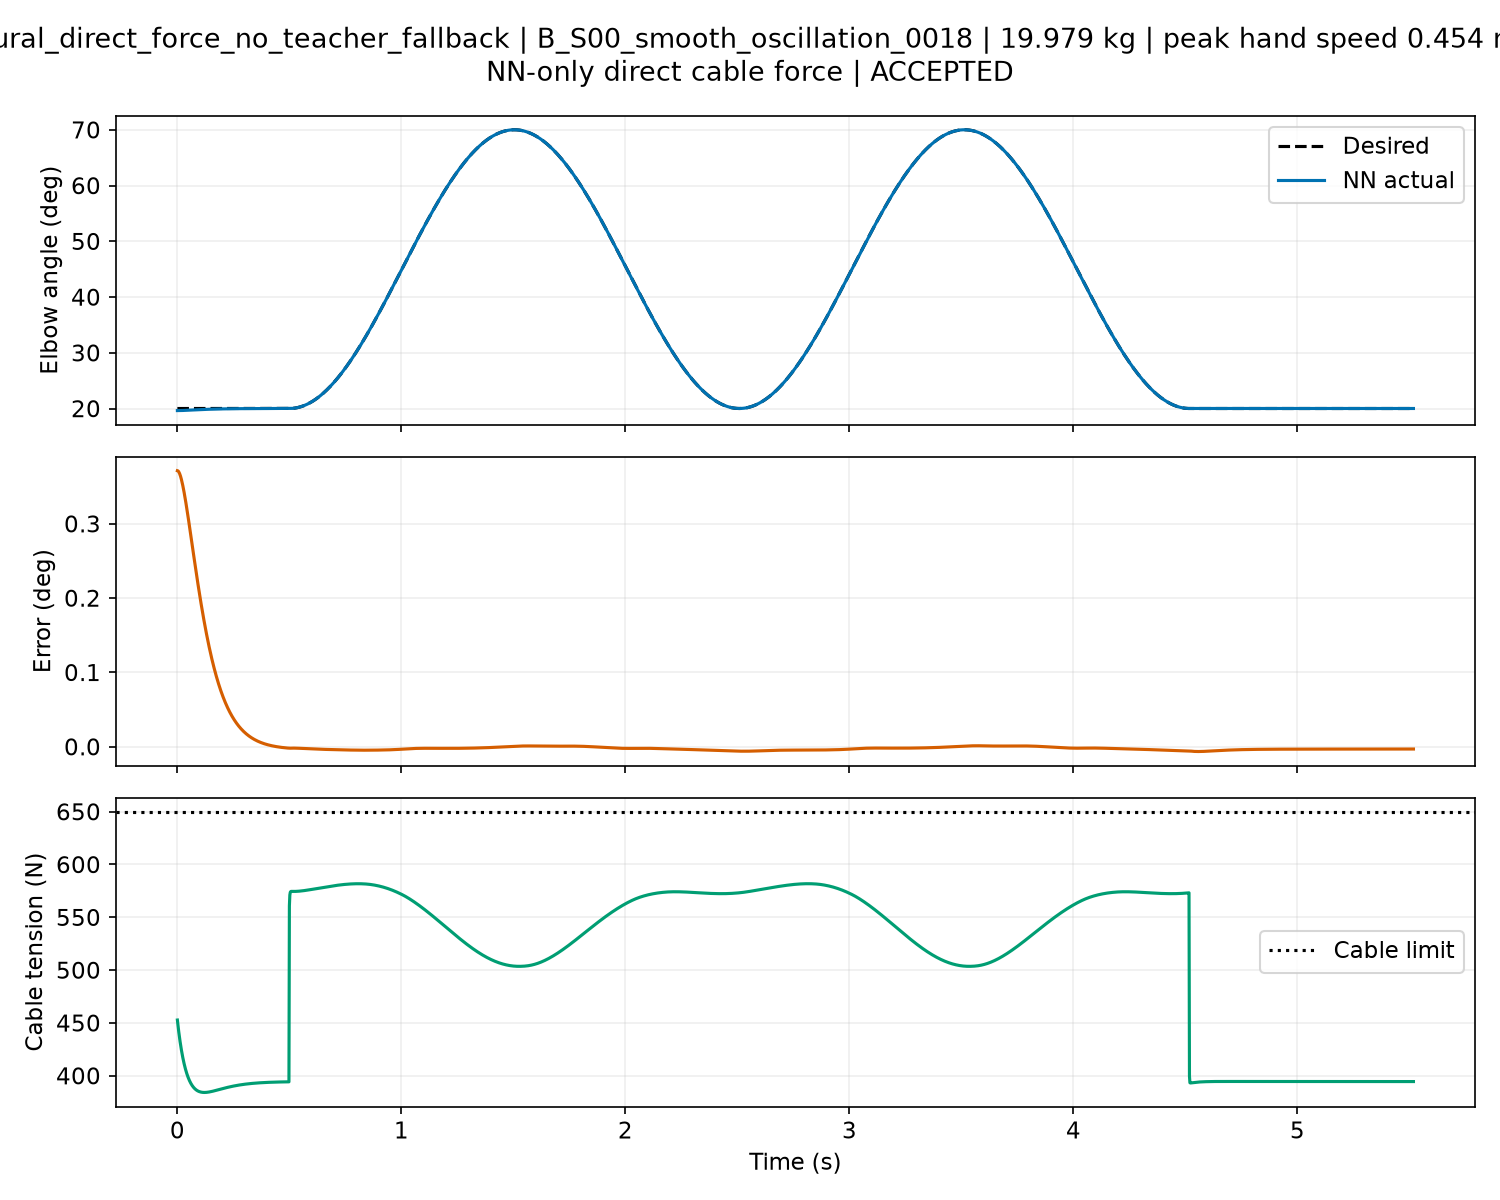
\includegraphics[width=\linewidth,height=0.69\textheight,keepaspectratio]{overleaf_figures/tracking_B_S00_smooth_oscillation_0018_tracking.png}
\caption{tracking/B\_S00\_smooth\_oscillation\_0018/tracking.png: Saved simulation diagnostics. Quantities and units are identified on the axes; failed runs are retained.}
\label{fig:tracking_B_S00_smooth_oscillation_0018_tracking}
\end{figure}